\documentclass[11pt,oneside,openright]{./style/phdthesis}

\usepackage{amsmath}
\usepackage[ansinew]{inputenc}
\usepackage[portuguese]{babel}
\usepackage[printonlyused, withpage]{acronym}
\usepackage{a4wide}
\usepackage{palatino}
\usepackage{fancyhdr}
\usepackage{fancybox}
\usepackage{amssymb}
%\usepackage{chapterbib} %com este package as referencias bibliográficas aparecem no final de cada capítulo
\usepackage{cite}
\usepackage{epsfig}
%\usepackage{subfigure}
\usepackage{graphics}
\usepackage{float}
\usepackage{here}
\usepackage[T1]{fontenc}
\usepackage{rotating}
\usepackage{multirow}
%\usepackage{comment}
%\usepackage{captionhack}
\usepackage{epigraph}
\usepackage[linkcolor=black]{hyperref}
%\renewcommand{\thesubfigure}{}
\hypersetup{colorlinks=true}
\usepackage{enumerate}
%\usepackage[numbers,sort&compress]{natbib}
%\usepackage{hypernat}
\usepackage{booktabs}
\usepackage{url}                    % needed to cite a site
\usepackage{eurosym}
\usepackage{makeidx}
\usepackage{datatool}
\usepackage[toc, acronym]{glossaries}
\usepackage{graphicx}
\usepackage{caption}
\usepackage{subcaption}

\usepackage{tabulary}
\usepackage{braket}

% subfile handling packages
\usepackage{subfiles}

\usepackage{multicol} 
\usepackage{tcolorbox}
\usepackage{booktabs}




\newcommand{\onlyinsubfile}[1]{#1}
\newcommand{\notinsubfile}[1]{}
\renewcommand{\textfraction}{0.01}
\renewcommand{\topfraction}{0.99}
\renewcommand{\floatpagefraction}{0.99}
\renewcommand{\bottomfraction}{0.99}
\renewcommand{\heavyrulewidth}{1pt}
\renewcommand{\lightrulewidth}{0.50pt}
\renewcommand{\chaptername}{Capítulo}
\renewcommand{\figurename}{Figura}
\renewcommand{\appendixname}{\Large{Anexo}}
\renewcommand{\tablename}{Tabela}
\renewcommand{\acronymname}{Acrónimos}

\newcommand{\mli}[1]{\mathit{#1}}
\newcommand{\intSpace}{\!\!\!\!}
\newcommand{\doubleInt}{\!\!\int\intSpace\int\!\!}
\newcommand{\TX}{\mathit{TX}}
\newcommand{\NLI}{\mathit{NLI}}
\newcommand{\eff}{\mathit{eff}}
\newcommand{\LOASE}{\mathit{LO-ASE}}
\newcommand{\LONLI}{\mathit{LO-NLI}}
\renewcommand{\kbldelim}{[}% Left delimiter
\renewcommand{\kbrdelim}{]}% Right delimiter

%\makesavenoteenv{tabular}



\hyphenpenalty=50000
\tolerance=10000
%%% General page formatting

\oddsidemargin 0.2in
\evensidemargin 0in
%\textwidth 155mm
\headheight 15.0pt
\topmargin 0in
%\textheight 237mm

% footheight 1.0in

\makeatletter
\providecommand*{\diff}%
{\@ifnextchar^{\DIfF}{\DIfF^{}}}
\def\DIfF^#1{%
\mathop{\mathrm{\mathstrut d}}%
\nolimits^{#1}\gobblespace}
\def\gobblespace{%
\futurelet\diffarg\opspace}
\def\opspace{%
\let\DiffSpace\!%
\ifx\diffarg(%
\let\DiffSpace\relax
\else
\ifx\diffarg[%
\let\DiffSpace\relax
\else
\ifx\diffarg\{%
\let\DiffSpace\relax
\fi\fi\fi\DiffSpace}

\providecommand*{\tDeriv}[3][]{%
\frac{\diff^{#1}#2}{\diff #3^{#1}}}
\providecommand*{\pDeriv}[3][]{%
\frac{\partial^{#1}#2}%
{\partial #3^{#1}}}

\graphicspath{{./figures/}}


\DeclareMathOperator{\erf}{erf}
\DeclareMathOperator{\erfc}{erfc}
\DeclareMathOperator{\sinc}{sinc}
\DeclareMathOperator{\R}{Re}
\DeclareMathOperator{\I}{Im}
\DeclareMathOperator{\asinh}{asinh}

%\newcommand{\publ}{}

\pagenumbering{arabic} 

\setcounter{MaxMatrixCols}{20}

\makeindex

\begin{document}
%%  include the LaTeX files containing the text for each chapters

% ------------------------------------------------------------------------
\title{NetXPTO - NetPlanner}
\author{}
\date{\today}
\maketitle
% ------------------------------------------------------------------------

% ------------------------------------------------------------------------fc
\tableofcontents
% ------------------------------------------------------------------------


\chapter{Introduction}
\label{introduction}

The amount of traffic, in particular IP traffic, has been increasing very substantially. This increase is due to the growing number of Internet-based applications, the increase in the number of devices connected to the Internet, the expansion of optical fiber to customers' homes, increased bandwidth of mobile access technologies, and increased of video traffic \cite{cisco}.
At the same time, with the increase in traffic, operators are under heavy pressure to reduce the cost per bit transported \cite{alcatel_lucent}. This implies the introduction of new technologies, which on the one hand increase the capacity of transport of the networks and on the other, reduce the costs of operation (OPEX) \cite{opexcapex}.
This process of technological conversion is operating in a macroeconomic scenario in which operators find it difficult to finance which forces them to have strong investment constraints (CAPEX) \cite{opexcapex}.
The transport networks have been predominantly based on circuit switching, either at the level of the optical channels or at the level of the electrical circuits, and the introduction of packet switching undermines this paradigm.


\newpage
%%%%%%%%%%%%%%%%%%%%%%%%%%%%%%%%%%%%%%%%%%%%%%%%%%%%%%%%%%%%%%%%%%%%%%%%
\section{Motivation and objectives}
\label{objectives}
Taking into account all these factors, the need to implement planning tools becomes important both for suppliers and operators and is used in the various stages of the telecommunications business.
These have a very important role and directly affect the competitiveness of operators.
One of the tools used for transport network planning is the integer linear programming models.
These models offer optimal solutions, however, some scalability limitations may arise. They also allow quick and easy changes.
Therefore this model becomes relevant in an environment where requirements may differ substantially between operators \cite{teserui}.\\
Due to the importance of transport network planning and design, this dissertation aims to achieve the following main objectives:

\begin{enumerate}
  \item Define one reference network and three different scenarios for performing tests.
  \item Develop ILP models for opaque, transparent and translucent networks without survivability and using 1+1 protection.
  \item Get analytical solutions for the previous point.
  \item Compare the analytical results and results based on ILP with the results obtained through heuristics.
\end{enumerate}


%%%%%%%%%%%%%%%%%%%%%%%%%%%%%%%%%%%%%%%%%%%%%%%%%%%%%%%%%%%%%%%%%%%%%%%%%%%%%%%%%%%%%%%
\section{Thesis outline}
\label{outline}

This thesis is organized in 7 chapters. Chapter \ref{chap_reference_network} consists of a state-of-art review about optical transport networks. In this chapter is also where the reference network used throughout the dissertation as well as the different traffics used is defined. The Chapter \ref{chap_capex} begins by determining the CAPEX calculation formula for use in the ILP model and for analytical calculations. The first section refers to ILP models and the other to analytical models. In Chapter \ref{chap_ilp} are several sections each for a particular mode of transport and certain survivability. In section \ref{ILP_Opaque_Survivability} we have opaque without survivability, in section \ref{ILP_Opaque_Protection} opaque with 1+1 protection. Sections \ref{ILP_Transp_Survivability} and \ref{ILP_Transp_Protection} relate to the transparent and lastly sections \ref{ILP_Transluc_Survivability} and \ref{ILP_Transluc_Protection} refer to the translucent. In the referred section it is possible to see the model description, the detailed description of the results and the conclusions of these results. The analytical calculation of all the models referred to in Chapter \ref{chap_ilp} can be found in Chapter \ref{chap_analytical}. In Chapter \ref{chap_comparative} the results obtained throughout this dissertation are compared and the chapter is divided into six sections where each corresponds to a certain mode of transport with their respective survivability. The last step is the conclusions \ref{chap_conclusions} and suggestions for future research directions.

%%%%%%%%%%%%%%%%%%%%%%%%%%%%%%%%%%%%%%%%%%%%%%%%%%%%%%%%%%%%%%%%%%%%%%%%%%%%%%%%%%%%%%%%%%%%%%%%%%%%%%%%%%%%%%%%%%%%%%%%%%%%%

% References
\phantomsection
\addcontentsline{toc}{section}{References}
%
\renewcommand{\bibname}{References}
%\bibliographystyle{IEEEtran}
%\bibliography{rmorais}
%
%
% Generated by IEEEtran.bst, version: 1.13 (2008/09/30)
\begin{thebibliography}{10}
\providecommand{\url}[1]{#1}
\csname url@samestyle\endcsname
\providecommand{\newblock}{\relax}
\providecommand{\bibinfo}[2]{#2}
\providecommand{\BIBentrySTDinterwordspacing}{\spaceskip=0pt\relax}
\providecommand{\BIBentryALTinterwordstretchfactor}{4}
\providecommand{\BIBentryALTinterwordspacing}{\spaceskip=\fontdimen2\font plus
\BIBentryALTinterwordstretchfactor\fontdimen3\font minus
  \fontdimen4\font\relax}
\providecommand{\BIBforeignlanguage}[2]{{%
\expandafter\ifx\csname l@#1\endcsname\relax
\typeout{** WARNING: IEEEtran.bst: No hyphenation pattern has been}%
\typeout{** loaded for the language `#1'. Using the pattern for}%
\typeout{** the default language instead.}%
\else
\language=\csname l@#1\endcsname
\fi
#2}}
\providecommand{\BIBdecl}{\relax}
\BIBdecl

\bibitem{cisco}
Cisco, ``Global Mobile Data Traffic Forecast Update 2015-2020,'' in \emph{Cisco Visual Networking Index}, pp. 2,3, 2016.

\bibitem{alcatel_lucent}
\BIBentryALTinterwordspacing
Alcatel-Lucent (2009). ``The new economics of telecom networks - bringing value back to the network,'' Tech. Rep. [Online]. Available:
  \url{http://images.tmcnet.com/online-communities/ngc/pdfs/application-enablement/whitepapers/The-New-Economics-of-Telecom-Networks.pdf}
\BIBentrySTDinterwordspacing

\bibitem{opexcapex}
S.~Verbrugge, D.~Colle, M.~Pickavet, P.~Demeester, S.~Pasqualini, A.~Iselt, A.~Kirst\"{a}dter, R.~H\"{u}lsermann, F.-J. Westphal, and M.~J\"{a}ger, ``Methodology and input availability parameters for calculating OpEx and CapEx costs for realistic network scenarios,'' \emph{Journal of Optical Networking}, vol.~5, no.~6, pp. 509--520, June 2006.

\bibitem{teserui}
R.~M.~D. Morais, ``Planning and Dimensioning of Multilayer Optical Transport Networks.'' PhD thesis, Universidade de Aveiro, 2015.

\end{thebibliography}


% ------------------------------------------------------------------------
\chapter{Simulator Structure}

LinkPlanner is a signals open-source simulator.

The major entity is the system.

A system comprises a set of blocks.

The blocks interact with each other through signals.

\section{System}

\section{Blocks}

\section{Signals}

List of available signals:

\begin{itemize}
    \item Signal

\end{itemize}










% ------------------------------------------------------------------------
\chapter{Development Cycle}

The NetXPTO-LinkPlanner has been developed by several people using git as a version control system.
The NetXPTO-LinkPlanner repository is located in the GitHub site http://github.com/netxpto/linkplanner.
The more updated functional version of the software is in the branch master.
Master should be considered a functional beta version of the software.
Periodically new releases are delivered from the master branch under the branch name Release<Year><Month><Day>.
The integration of the work of all people is performed by Armando Nolasco Pinto in the branch Develop.
Each developer has is how branch with his/her name.





% ------------------------------------------------------------------------
\chapter{Network specification}
\label{chap_reference_network}
The purpose of this chapter is to describe a state-of-art review about optical transport networks and finally describe a reference network that will be used for the various types of dimensioning throughout this dissertation. In addition to the reference network will also be described the various traffic models used in this network in question.\\
The organization of this chapter is done by creating four subsections, the first \ref{network_components} refers to the components of the network, the second \ref{network_topologies} depicts the topologies of the network and in the third \ref{transport_mode} it is possible to describe the different types of mode of transport. At the end, in the \ref{reference_network} is described the physical topology of the network and how to create the traffic matrix for the three existing traffic models (low, medium and high traffic).\\


% ------------------------------------------------------------------------
\chapter{Network specification}
\label{chap_reference_network}
The purpose of this chapter is to describe a state-of-art review about optical transport networks and finally describe a reference network that will be used for the various types of dimensioning throughout this dissertation. In addition to the reference network will also be described the various traffic models used in this network in question.\\
The organization of this chapter is done by creating four subsections, the first \ref{network_components} refers to the components of the network, the second \ref{network_topologies} depicts the topologies of the network and in the third \ref{transport_mode} it is possible to describe the different types of mode of transport. At the end, in the \ref{reference_network} is described the physical topology of the network and how to create the traffic matrix for the three existing traffic models (low, medium and high traffic).\\


% ------------------------------------------------------------------------
\chapter{Network specification}
\label{chap_reference_network}
The purpose of this chapter is to describe a state-of-art review about optical transport networks and finally describe a reference network that will be used for the various types of dimensioning throughout this dissertation. In addition to the reference network will also be described the various traffic models used in this network in question.\\
The organization of this chapter is done by creating four subsections, the first \ref{network_components} refers to the components of the network, the second \ref{network_topologies} depicts the topologies of the network and in the third \ref{transport_mode} it is possible to describe the different types of mode of transport. At the end, in the \ref{reference_network} is described the physical topology of the network and how to create the traffic matrix for the three existing traffic models (low, medium and high traffic).\\

\input{./sdf/reference_network/reference_network}

%%%%%%%%%%%%%%%%%%%%%%%%%%%%%%%%%%%%%%%%%%%%%%%%%%%%%%%%%%%%%%%%%%%%%%%%%%%%%%%%%%%%%%%%%%%%%%%%%%%%%%%%%%%%%%%%%%%%%%%%%%%%%

% References
\phantomsection
\addcontentsline{toc}{section}{References}
%
\renewcommand{\bibname}{References}
%\bibliographystyle{IEEEtran}
%\bibliography{rmorais}
%
%
% Generated by IEEEtran.bst, version: 1.13 (2008/09/30)
\begin{thebibliography}{10}
\providecommand{\url}[1]{#1}
\csname url@samestyle\endcsname
\providecommand{\newblock}{\relax}
\providecommand{\bibinfo}[2]{#2}
\providecommand{\BIBentrySTDinterwordspacing}{\spaceskip=0pt\relax}
\providecommand{\BIBentryALTinterwordstretchfactor}{4}
\providecommand{\BIBentryALTinterwordspacing}{\spaceskip=\fontdimen2\font plus
\BIBentryALTinterwordstretchfactor\fontdimen3\font minus
  \fontdimen4\font\relax}
\providecommand{\BIBforeignlanguage}[2]{{%
\expandafter\ifx\csname l@#1\endcsname\relax
\typeout{** WARNING: IEEEtran.bst: No hyphenation pattern has been}%
\typeout{** loaded for the language `#1'. Using the pattern for}%
\typeout{** the default language instead.}%
\else
\language=\csname l@#1\endcsname
\fi
#2}}
\providecommand{\BIBdecl}{\relax}
\BIBdecl

\bibitem{book07}
E.~Bouillet, G.~Ellinas, J.-F. Labourdette, and R.~Ramamurthy, \emph{Path Routing in Mesh Optical Networks}, John Wiley \& Sons, 2007.

\bibitem{ramas2010}
R. Ramaswami, K. N.~Sivarajan, and G. H. Sasaki, \emph{Optical Networks: A Practical Perspective}, Morgan Kaufmann, 2010.

\bibitem{tesevasco}
V.~R.~B.~S. Braz, ``Dimensioning and Optimization of Node Architecture in Optical Transport Networks.'' Master's thesis, Universidade de Aveiro, 2016.

\bibitem{teserui}
R.~M.~D. Morais, ``Planning and Dimensioning of Multilayer Optical Transport Networks.'' PhD thesis, Universidade de Aveiro, 2015.

\bibitem{aulas2}
A.~N. Pinto, ``Optical Networks - Topology,'' in \emph{Aulas de redes opticas 2016-2017.}

\bibitem{teselisboa}
A.~M.~P. Fernandes, ``Estratégias de Planeamento para Tráfego Estático e Dinâmico em Redes de Transporte Óticas.'' Master's thesis, Universidade de Lisboa, 2017.

\bibitem{opaque}
A. Autenrieth, A.~K. Tilwankar, C.~M. Machuca, and J.~P. Elbers, ``Power consumption analysis of opaque and transparent optical core networks.'' in \emph{Proc. 13th Int. Conf. Transparent Optical Networks}, pp. 1-5, June 2011.

\bibitem{transparent}
H. Abdalla, H.~A.~F. Crispim, E.~T.~L. Pastor, A.~J.~M. Soares, and L.~A. Bermudez, ``Optical transparent IP/WDM network simulation,'' in \emph{Proc. SBMO/IEEE MTT-S Int. Conf. Microwave and Optoelectronics}, pp. 19-23, July 2005.

\bibitem{zhu}
K. Zhu, H. Zhu, and B. Mukherjee, ``Traffic Grooming in an Optical WDM Mesh Network,'' Springer, 2002.

\bibitem{alcatel}
\BIBentryALTinterwordspacing
Alcatel-Lucent (2010). ``Understanding OTN Optical Transport Network (G.709), March 9, 2010'' [Online]. Available:
  \url{http://www.cvt-dallas.org/March2010.pdf}
\BIBentrySTDinterwordspacing

\end{thebibliography} 

%%%%%%%%%%%%%%%%%%%%%%%%%%%%%%%%%%%%%%%%%%%%%%%%%%%%%%%%%%%%%%%%%%%%%%%%%%%%%%%%%%%%%%%%%%%%%%%%%%%%%%%%%%%%%%%%%%%%%%%%%%%%%

% References
\phantomsection
\addcontentsline{toc}{section}{References}
%
\renewcommand{\bibname}{References}
%\bibliographystyle{IEEEtran}
%\bibliography{rmorais}
%
%
% Generated by IEEEtran.bst, version: 1.13 (2008/09/30)
\begin{thebibliography}{10}
\providecommand{\url}[1]{#1}
\csname url@samestyle\endcsname
\providecommand{\newblock}{\relax}
\providecommand{\bibinfo}[2]{#2}
\providecommand{\BIBentrySTDinterwordspacing}{\spaceskip=0pt\relax}
\providecommand{\BIBentryALTinterwordstretchfactor}{4}
\providecommand{\BIBentryALTinterwordspacing}{\spaceskip=\fontdimen2\font plus
\BIBentryALTinterwordstretchfactor\fontdimen3\font minus
  \fontdimen4\font\relax}
\providecommand{\BIBforeignlanguage}[2]{{%
\expandafter\ifx\csname l@#1\endcsname\relax
\typeout{** WARNING: IEEEtran.bst: No hyphenation pattern has been}%
\typeout{** loaded for the language `#1'. Using the pattern for}%
\typeout{** the default language instead.}%
\else
\language=\csname l@#1\endcsname
\fi
#2}}
\providecommand{\BIBdecl}{\relax}
\BIBdecl

\bibitem{book07}
E.~Bouillet, G.~Ellinas, J.-F. Labourdette, and R.~Ramamurthy, \emph{Path Routing in Mesh Optical Networks}, John Wiley \& Sons, 2007.

\bibitem{ramas2010}
R. Ramaswami, K. N.~Sivarajan, and G. H. Sasaki, \emph{Optical Networks: A Practical Perspective}, Morgan Kaufmann, 2010.

\bibitem{tesevasco}
V.~R.~B.~S. Braz, ``Dimensioning and Optimization of Node Architecture in Optical Transport Networks.'' Master's thesis, Universidade de Aveiro, 2016.

\bibitem{teserui}
R.~M.~D. Morais, ``Planning and Dimensioning of Multilayer Optical Transport Networks.'' PhD thesis, Universidade de Aveiro, 2015.

\bibitem{aulas2}
A.~N. Pinto, ``Optical Networks - Topology,'' in \emph{Aulas de redes opticas 2016-2017.}

\bibitem{teselisboa}
A.~M.~P. Fernandes, ``Estratégias de Planeamento para Tráfego Estático e Dinâmico em Redes de Transporte Óticas.'' Master's thesis, Universidade de Lisboa, 2017.

\bibitem{opaque}
A. Autenrieth, A.~K. Tilwankar, C.~M. Machuca, and J.~P. Elbers, ``Power consumption analysis of opaque and transparent optical core networks.'' in \emph{Proc. 13th Int. Conf. Transparent Optical Networks}, pp. 1-5, June 2011.

\bibitem{transparent}
H. Abdalla, H.~A.~F. Crispim, E.~T.~L. Pastor, A.~J.~M. Soares, and L.~A. Bermudez, ``Optical transparent IP/WDM network simulation,'' in \emph{Proc. SBMO/IEEE MTT-S Int. Conf. Microwave and Optoelectronics}, pp. 19-23, July 2005.

\bibitem{zhu}
K. Zhu, H. Zhu, and B. Mukherjee, ``Traffic Grooming in an Optical WDM Mesh Network,'' Springer, 2002.

\bibitem{alcatel}
\BIBentryALTinterwordspacing
Alcatel-Lucent (2010). ``Understanding OTN Optical Transport Network (G.709), March 9, 2010'' [Online]. Available:
  \url{http://www.cvt-dallas.org/March2010.pdf}
\BIBentrySTDinterwordspacing

\end{thebibliography} 

%%%%%%%%%%%%%%%%%%%%%%%%%%%%%%%%%%%%%%%%%%%%%%%%%%%%%%%%%%%%%%%%%%%%%%%%%%%%%%%%%%%%%%%%%%%%%%%%%%%%%%%%%%%%%%%%%%%%%%%%%%%%%

% References
\phantomsection
\addcontentsline{toc}{section}{References}
%
\renewcommand{\bibname}{References}
%\bibliographystyle{IEEEtran}
%\bibliography{rmorais}
%
%
% Generated by IEEEtran.bst, version: 1.13 (2008/09/30)
\begin{thebibliography}{10}
\providecommand{\url}[1]{#1}
\csname url@samestyle\endcsname
\providecommand{\newblock}{\relax}
\providecommand{\bibinfo}[2]{#2}
\providecommand{\BIBentrySTDinterwordspacing}{\spaceskip=0pt\relax}
\providecommand{\BIBentryALTinterwordstretchfactor}{4}
\providecommand{\BIBentryALTinterwordspacing}{\spaceskip=\fontdimen2\font plus
\BIBentryALTinterwordstretchfactor\fontdimen3\font minus
  \fontdimen4\font\relax}
\providecommand{\BIBforeignlanguage}[2]{{%
\expandafter\ifx\csname l@#1\endcsname\relax
\typeout{** WARNING: IEEEtran.bst: No hyphenation pattern has been}%
\typeout{** loaded for the language `#1'. Using the pattern for}%
\typeout{** the default language instead.}%
\else
\language=\csname l@#1\endcsname
\fi
#2}}
\providecommand{\BIBdecl}{\relax}
\BIBdecl

\bibitem{book07}
E.~Bouillet, G.~Ellinas, J.-F. Labourdette, and R.~Ramamurthy, \emph{Path Routing in Mesh Optical Networks}, John Wiley \& Sons, 2007.

\bibitem{ramas2010}
R. Ramaswami, K. N.~Sivarajan, and G. H. Sasaki, \emph{Optical Networks: A Practical Perspective}, Morgan Kaufmann, 2010.

\bibitem{tesevasco}
V.~R.~B.~S. Braz, ``Dimensioning and Optimization of Node Architecture in Optical Transport Networks.'' Master's thesis, Universidade de Aveiro, 2016.

\bibitem{teserui}
R.~M.~D. Morais, ``Planning and Dimensioning of Multilayer Optical Transport Networks.'' PhD thesis, Universidade de Aveiro, 2015.

\bibitem{aulas2}
A.~N. Pinto, ``Optical Networks - Topology,'' in \emph{Aulas de redes opticas 2016-2017.}

\bibitem{teselisboa}
A.~M.~P. Fernandes, ``Estratégias de Planeamento para Tráfego Estático e Dinâmico em Redes de Transporte Óticas.'' Master's thesis, Universidade de Lisboa, 2017.

\bibitem{opaque}
A. Autenrieth, A.~K. Tilwankar, C.~M. Machuca, and J.~P. Elbers, ``Power consumption analysis of opaque and transparent optical core networks.'' in \emph{Proc. 13th Int. Conf. Transparent Optical Networks}, pp. 1-5, June 2011.

\bibitem{transparent}
H. Abdalla, H.~A.~F. Crispim, E.~T.~L. Pastor, A.~J.~M. Soares, and L.~A. Bermudez, ``Optical transparent IP/WDM network simulation,'' in \emph{Proc. SBMO/IEEE MTT-S Int. Conf. Microwave and Optoelectronics}, pp. 19-23, July 2005.

\bibitem{zhu}
K. Zhu, H. Zhu, and B. Mukherjee, ``Traffic Grooming in an Optical WDM Mesh Network,'' Springer, 2002.

\bibitem{alcatel}
\BIBentryALTinterwordspacing
Alcatel-Lucent (2010). ``Understanding OTN Optical Transport Network (G.709), March 9, 2010'' [Online]. Available:
  \url{http://www.cvt-dallas.org/March2010.pdf}
\BIBentrySTDinterwordspacing

\end{thebibliography} 
%
% ------------------------------------------------------------------------
\chapter{Integer linear programming}
\label{chap_ilp}
ILP models are used to design networks that describe real components and their capabilities through a set of linear equations. Despite their quality, the solutions obtained through these models, depending on the number of variables and computational resources, can take days, months or even years \cite{ILP01}.
The current chapter proposes and describes the optimization models used to calculating the capital expenditures of the network, based on the three modes of transport (opaque, transparent and translucent) without survivability and protection.
In the first section the introduction to ILP models is made.
Next, in the following sections it is proposed in detail the restrictions of the three models previously mentioned, without survivability and with protection as well as a detailed report of the obtained results for each case.
Finally in the last section all the general conclusions of these models are described.

%%%%%%%%%%%%%%%%%%%%%%%%%%%%%%%%%%%%%%%%%%%%%%%%%%%%%%%%%%%%%%%%%%%%%%%%%%%%%%%%%%%%%%%%%%%%%%%%%%%%%%%%%%%%%%%%%%%%
\newpage
\section{Introduction of ILP models}

The development of an ILP model first requires the definition of the inputs, outputs and variables of the problem in a mathematical representation.
Regarding the input parameters for this work we will consider the reference network described in \ref{Reference_Network_Topology} where the network connections are in the form of an adjacency matrix called $G_{ij}$.
Also as input parameter we take into account bidirectional demand matrices $D_{odc}$ created in section \ref{Reference_Network_Traffic} for each type of client traffic with $c = [1;2;3;4;5]$ depending on the ODU, where 1 corresponds to ODU0 and 5 to ODU4.\\

The main objective is to determine the values of the decision variables, so that all linear equations are satisfied and the value of the objective function is minimized. The objective function is introduced by the keyword "minimize" and the constraint set is introduced by the expression "subject to".
To perform the implementation of the models it is necessary to use a mathematical software tool. For this we will use MATLAB which is ideal for dealing with linear programming problems and can call the LPsolve through an external interface \cite{tesevasco,opaqueILP}. In the following sections the ILP model is presented in detail for each transport mode.\\
%%%%%%%%%%%%%%%%%%%%%%%%%%%%%%%%%%%%%%%%%%%%%%%%%%%%%%%%%%%%%%%%%%%%%%%%%%%%%%%%%%%%%%%%%%%%%%%%%%%%%%%%%%%%%%%%%%%%

%Subsection with the different transport mode

\section{Opaque without survivability}\label{ILP_Opaque_Survivability}

\subsection{Model description}

In order to be able to apply the ILP model we have to take into account the physical and logical topologies allowed by this mode of transport and the type of survivability. Based on what was mentioned in section \ref{opaque} on this mode of transport we can conclude that both topologies are the same and the following figures can be confirmed.\\

\begin{figure}[h!]
\centering
\includegraphics[width=10cm]{sdf/ilp/opaque_survivability/figures/allowed_physical_topology}
\caption{Opaque without survivability: allowed physical topology. The allowed physical topology is defined by the duct and sites in the field. It is assumed that each duct supports up to 1 bidirectional transmission system and each site supports up to 1 node.}
\label{allowed_physical_low}
\end{figure}

\newpage
\begin{figure}[h!]
\centering
\includegraphics[width=10cm]{sdf/ilp/opaque_survivability/figures/allowed_optical_topology}
\caption{Opaque without survivability: allowed optical topology. The allowed optical topology is defined by the transport mode. It is assumed that each transmission system supports up to 100 optical channels.}
\label{allowed_optical_low}
\end{figure}

Now taking this into account and based on the specific constraints of the opaque mode without survivability it is possible to define the ILP model \cite{aularui}.\\

The objective function, to be minimized, is the expression \ref{Capex},

\begin{equation}
  minimize \qquad \Big\{ \quad C_C \quad \Big\}
  \label{ILPOpaque_CAPEX}
\end{equation}

$subject$ $to$
\begin{equation}
\sum_{j=1\textbackslash \{o\}}^{N} fb_{ij}^{od} = 1  \qquad \qquad \qquad \qquad \qquad \qquad \qquad \qquad \qquad
\forall(o,d) : o < d, \forall i: i = o
\label{ILPOpaque1_Surv}
\end{equation}
\noindent
Constraint \ref{ILPOpaque1_Surv} is equal to the constraint \ref{ILPOpaque1_CAPEX} assuming that Z = 1.

\begin{equation}
\sum_{j=1\textbackslash \{o\}}^{N} fb_{ij}^{od} = \sum_{j=1\textbackslash \{d\}}^{N} f_{ji}^{od}   \qquad \qquad \qquad \qquad \qquad \qquad
\forall(o,d) : o < d, \forall i: i \neq o,d
\label{ILPOpaque2_Surv}
\end{equation}
\noindent
Constraint \ref{ILPOpaque2_Surv} is equal to the constraint \ref{ILPOpaque2_CAPEX}.

\begin{equation}
\sum_{j=1\textbackslash \{d\}}^{N} fb_{ji}^{od} = 1  \qquad \qquad \qquad \qquad \qquad \qquad \qquad \qquad \qquad
\forall(o,d) : o < d, \forall i: i = d
\label{ILPOpaque3_Surv}
\end{equation}
\noindent
Constraint \ref{ILPOpaque3_Surv} is equal to the constraint \ref{ILPOpaque3_CAPEX} assuming that Z = 1.

\begin{equation}
\sum_{o=1}^{N} \sum_{d=o+1}^{N} \left(fb_{ij}^{od} + fb_{ji}^{od}\right) \sum_{c=1}^{C} (B\left(c\right) D_{odc})\leq \tau W_{ij} G_{ij} \qquad \qquad \qquad \qquad
\forall(i,j) : i < j
\label{ILPOpaque4_Surv}
\end{equation}
\noindent
The constraint \ref{ILPOpaque4_Surv} is considered the grooming constraint, so it means that the total client traffic flows can not be greater than the capacity of the line bit rate. Where $\tau$ is the line bit rate. In this work we assume that $\tau$ = 100 Gbits/s. $G_{ij}$ is the adjacency matrix, which means that we can only use a connection if it exists in the physical topology of the network.

\begin{equation}
W_{ij} \leq K_{ij} L_{ij} \qquad  \qquad \qquad \qquad \qquad \qquad \qquad \qquad \qquad \qquad \qquad \qquad \forall(i,j) : i < j
\label{ILPOpaque5_Surv}
\end{equation}
\noindent
Constraint \ref{ILPOpaque5_Surv} concerns the capacity of the optical channels which must be less or equal than the maximum number of optical channels. For any situation the maximum number of optical channels supported by each transmission system is 100, i.e., $K_{ij}$ = 100.

\begin{equation}
fb_{ij}^{od} , fb_{ji}^{od}, L_{ij} \in \{0,1\}   \qquad \qquad \qquad \qquad \qquad \qquad \qquad
\forall(i,j) : i < j, \forall(o,d) : o < d
\label{ILPOpaque6_Surv}
\end{equation}
\noindent
Constraint \ref{ILPOpaque6_Surv} define the variables $fb$ and $L_{ij}$ as binary values.

\begin{equation}
W_{ij} \in \mathbb{N}  \qquad \qquad \qquad \qquad \qquad \qquad \qquad \qquad \qquad \qquad \qquad \qquad \qquad
\forall(i,j) : i < j
\label{ILPOpaque7_Surv}
\end{equation}
\noindent
This constraint defines the variables $W_{ij}$ as integer variables allowing that between each pair of nodes can exist more that one lightpath.

\subsection{Result description}

\textbf{Low Traffic Scenario:}\\

In a first phase, we will show the resulting physical and optical topology. These topologies are based on the allowed topologies referred to in the model description and also taking into account the logical topology for all ODUs mentioned in the section \ref{low_scenario}.

\begin{figure}[h!]
\centering
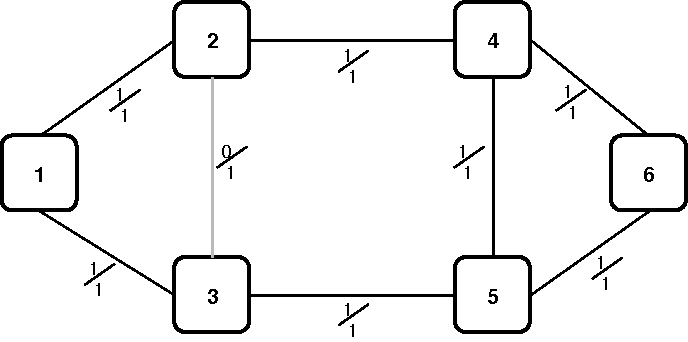
\includegraphics[width=11cm]{sdf/ilp/opaque_survivability/figures/physical_topology_low}
\caption{Opaque without survivability in low scenario: physical topology after dimensioning.}
\label{physical_low}
\end{figure}
\newpage
\begin{figure}[h!]
\centering
\includegraphics[width=11cm]{sdf/ilp/opaque_survivability/figures/optical_topology_low}
\caption{Opaque without survivability in low scenario: optical topology after dimensioning.}
\label{optical_low}
\end{figure}

In table \ref{link_opaque_surv_ref_low} we can see the number of optical channels calculated using \ref{Capex_Link} and \ref{ILPOpaque_CAPEX} and the number of amplifiers for each link calculated using \ref{Capex_amplifiers}. In the case where there are no optical channels we assume that the number of amplifiers is zero.

\begin{table}[h!]
\centering
\begin{tabular}{|| c | c | c ||}
 \hline
 \multicolumn{3}{|| c ||}{Information regarding links} \\
 \hline
 \hline
 Bidirectional Link & Optical Channels & Amplifiers\\
 \hline
 Node 1 <-> Node 2 & 1 & 4 \\
 Node 1 <-> Node 3 & 0 & 0 \\
 Node 2 <-> Node 3 & 1 & 0 \\
 Node 2 <-> Node 4 & 2 & 6 \\
 Node 3 <-> Node 5 & 1 & 8 \\
 Node 4 <-> Node 5 & 0 & 0 \\
 Node 4 <-> Node 6 & 2 & 7 \\
 Node 5 <-> Node 6 & 2 & 3 \\
 \hline
\end{tabular}
\caption{Table with information regarding links for opaque mode without survivability in low scenario.}
\label{link_opaque_surv_ref_low}
\end{table}

In table \ref{node_opaque_surv_ref_low} we can see the resulting nodal degree at the physical layer, calculated based on the number of connections that the node in question performs, the number of line ports calculated using \ref{EXC_pexc1_opaque} and the number of tributary ports calculated using \ref{EXC_pexc2_opaque} for each node.

\begin{table}[h!]
\centering
\begin{tabular}{|| c | c | c | c ||}
 \hline
 \multicolumn{4}{|| c ||}{Information regarding nodes} \\
 \hline
 \hline
 Node & Resulting Nodal Degree & Line Ports & Tributary Ports\\
 \hline
 1 & 1 & 1 & 29 \\
 2 & 3 & 4 & 23 \\
 3 & 2 & 2 & 18 \\
 4 & 2 & 4 & 20 \\
 5 & 2 & 3 & 24 \\
 6 & 2 & 4 & 22 \\
\hline
\end{tabular}
\caption{Table with information regarding nodes for opaque mode without survivability in low scenario.}
\label{node_opaque_surv_ref_low}
\end{table}

\newpage
Through the information obtained previously on the nodes we can now create tables with detailed information about each node. In each table mentioned below we can see how many ports are connected to a given node and its bit rate (in relation to the line ports) and how many ports are assigned to each different bit rate (in relation to the tributary ports).

\begin{table}[h!]
\centering
\begin{tabular}{|| c | c | c ||}
 \hline
 \multicolumn{3}{|| c ||}{Detailed description of Node 1} \\
 \hline
 \hline
  & Number of total demands & Bit rate \\
 \hline
 \multirow{3}{*}{29 tributary ports} & 13 & ODU0 \\
 & 13 & ODU1 \\
 & 3 & ODU2 \\
 \hline
 \hline
  & Node<--Optical Channels-->Node & Bit rate \\
 \hline
 1 line ports & 1  <---- 1 ---->  2 & 100 Gbits/s \\
\hline
\end{tabular}
\caption{Opaque without survivability in low scenario: detailed description of node 1. The number of demands is distributed to the various destination nodes, and can be observed in section \ref{low_scenario}.}
\end{table}

\begin{table}[h!]
\centering
\begin{tabular}{|| c | c | c ||}
 \hline
 \multicolumn{3}{|| c ||}{Detailed description of Node 2} \\
 \hline
 \hline
  & Number of total demands & Bit rate \\ \hline
 \multirow{5}{*}{23 tributary ports} & 11 & ODU0 \\
 & 7 & ODU1 \\
 & 2 & ODU2 \\
 & 2 & ODU3 \\
 & 1 & ODU4 \\
 \hline
 \hline
  & Node<--Optical Channels-->Node & Bit rate \\ \hline
 \multirow{3}{*}{4 line ports} & 2  <---- 1 ---->  1 & \multirow{3}{*}{100 Gbits/s} \\
 & 2  <---- 1 ---->  3 & \\
 & 2  <---- 2 ---->  4 & \\
\hline
\end{tabular}
\caption{Opaque without survivability in low scenario: detailed description of node 2. The number of demands is distributed to the various destination nodes, and can be observed in section \ref{low_scenario}.}
\end{table}

\begin{table}[h!]
\centering
\begin{tabular}{|| c | c | c ||}
 \hline
 \multicolumn{3}{|| c ||}{Detailed description of Node 3} \\
 \hline
 \hline
  & Number of total demands & Bit rate \\ \hline
 \multirow{4}{*}{18 tributary ports} & 7 & ODU0 \\
 & 6 & ODU1\\
 & 3 & ODU2\\
 & 2 & ODU3\\
 \hline
 \hline
  & Node<--Optical Channels-->Node & Bit rate \\
 \hline
 \multirow{2}{*}{2 line ports} & 3  <---- 1 ---->  2 & \multirow{2}{*}{100 Gbits/s}\\
 & 3  <---- 1 ---->  5 & \\
\hline
\end{tabular}
\caption{Opaque without survivability in low scenario: detailed description of node 3. The number of demands is distributed to the various destination nodes, and can be observed in section \ref{low_scenario}.}
\end{table}

\newpage
\begin{table}[h!]
\centering
\begin{tabular}{|| c | c | c ||}
 \hline
 \multicolumn{3}{|| c ||}{Detailed description of Node 4} \\
 \hline
 \hline
  & Number of total demands & Bit rate \\ \hline
 \multirow{3}{*}{20 tributary ports} & 7 & ODU0 \\
 & 10 & ODU1 \\
 & 3 & ODU2 \\
 \hline
 \hline
  & Node<--Optical Channels-->Node & Bit rate \\
 \hline
 \multirow{2}{*}{4 line ports} & 4  <---- 2 ---- >  2 & \multirow{2}{*}{100 Gbits/s}\\
 & 4  <---- 2 ----> 6 & \\
\hline
\end{tabular}
\caption{Opaque without survivability in low scenario: detailed description of node 4. The number of demands is distributed to the various destination nodes, and can be observed in section \ref{low_scenario}.}
\end{table}

\begin{table}[h!]
\centering
\begin{tabular}{|| c | c | c ||}
 \hline
 \multicolumn{3}{|| c ||}{Detailed description of Node 5} \\
 \hline
 \hline
  & Number of total demands & Bit rate \\ \hline
 \multirow{5}{*}{24 tributary ports} & 14 & ODU0 \\
 & 4 & ODU1 \\
 & 4 & ODU2 \\
 & 1 & ODU3 \\
 & 1 & ODU4 \\
 \hline
 \hline
  & Node<--Optical Channels-->Node & Bit rate \\
 \hline
 \multirow{2}{*}{3 line ports} & 5  <---- 1 ---->  3 & \multirow{2}{*}{100 Gbits/s}\\
 & 5  <---- 2 ---->  6 & \\
 \hline
\end{tabular}
\caption{Opaque without survivability in low scenario: detailed description of node 5. The number of demands is distributed to the various destination nodes, and can be observed in section \ref{low_scenario}.}
\end{table}

\begin{table}[h!]
\centering
\begin{tabular}{|| c | c | c ||}
 \hline
 \multicolumn{3}{|| c ||}{Detailed description of Node 6} \\
 \hline
 \hline
  & Number of total demands & Bit rate \\
 \hline
 \multirow{5}{*}{22 tributary ports} & 8 & ODU0 \\
 & 10 & ODU1 \\
 & 1 & ODU2 \\
 & 1 & ODU3 \\
 & 2 & ODU4 \\
 \hline
 \hline
  & Node<--Optical Channels-->Node & Bit rate \\
 \hline
 \multirow{2}{*}{4 line ports} & 6  <---- 2 ---->  4 & \multirow{2}{*}{100 Gbits/s}\\
 & 6  <---- 2 ---->  5 & \\
\hline
\end{tabular}
\caption{Opaque without survivability in low scenario: detailed description of node 6. The number of demands is distributed to the various destination nodes, and can be observed in section \ref{low_scenario}.}
\end{table}

\vspace{15pt}
In next step let's focus on the routing information. These paths are bidirectional so the path from one node to another is the same path in the opposite direction. In table \ref{path_opaque_surv_ref_low} we can see all the routing obtained for all nodes.\\
\newpage
\begin{table}[h!]
\centering
\begin{tabular}{|| c | c | c | c | c | c | c | c ||}
 \hline
 \multicolumn{8}{|| c ||}{Routing} \\
 \hline
 \hline
 o & d & Links & ODU0 & ODU1 & ODU2 & ODU3 & ODU4 \\
 \hline
 1 & 2 & \{(1,2)\} & 5 & 2 & 1 & 0 & 0 \\ \hline
 1 & 3 & \{(1,2),(2,3)\} & 1 & 4 & 1 & 0 & 0\\ \hline
 1 & 4 & \{(1,2),(2,4)\} & 3 & 2 & 1 & 0 & 0\\ \hline
 1 & 5 & \{(1,2),(2,3),(3,5)\} & 1 & 0 & 0 & 0 & 0\\ \hline
 1 & 6 & \{(1,2),(2,4),(4,6)\} & 3 & 5 & 0 & 0 & 0\\ \hline
 2 & 3 & \{(2,3)\} & 0 & 0 & 0 & 1 & 0 \\ \hline
 2 & 4 & \{(2,4)\} & 1 & 3 & 0 & 0 & 0\\ \hline
 2 & 5 & \{(2,3),(3,5)\} & 5 & 1 & 1 & 0 & 0 \\ \hline
 2 & 6 & \{(2,4),(4,6)\} & 0 & 1 & 0 & 1 & 1 \\ \hline
 3 & 4 & \{(3,2),(2,4)\} & 1 & 1 & 1 & 0 & 0 \\ \hline
 3 & 5 & \{(3,5)\} & 4 & 1 & 1 & 1 & 0 \\ \hline
 3 & 6 & \{(3,5),(5,6)\} & 1 & 0 & 0 & 0 & 0\\ \hline
 4 & 5 & \{(4,6),(6,5)\} & 1 & 1 & 1 & 0 & 0\\ \hline
 4 & 6 & \{(4,6)\} & 1 & 3 & 0 & 0 & 0\\ \hline
 5 & 6 & \{(5,6)\} & 3 & 1 & 1 & 0 & 1\\
 \hline
\end{tabular}
\caption{Opaque without survivability in low scenario: description of demands routing. We are assuming that between a pair of nodes all demands follow the same route.}
\label{path_opaque_surv_ref_low}
\end{table}

Finally and most importantly through table \ref{scriptopaque_surv_ref_low} we can see the CAPEX result for this model. All the values calculated in the next table were obtained through the equations \ref{Capex_Link} and \ref{Capex_Node} referred to in section \ref{ILP_CAPEX}.

\begin{table}[h!]
\centering
\begin{tabular}{||c|c|c|c|c|c|c||}
 \hline
 \multicolumn{7}{||c||}{CAPEX of the Network} \\
 \hline
 \hline
 \multicolumn{3}{||c|}{ }&Quantity&Unit Price&Cost&Total \\
 \hline
 \multirow{3}{*}{Link Cost}&\multicolumn{2}{c|}{OLTs}&12&15 000 \euro&180 000 \euro&\multirow{3}{*}{9 404 000 \euro} \\ \cline{2-6}
 &\multicolumn{2}{c|}{100 Gbits/s Transceivers}&18&5 000 \euro/Gbit/s&9 000 000 \euro&\\ \cline{2-6}
 &\multicolumn{2}{c|}{Amplifiers}&56&4 000 \euro&224 000 \euro&\\
 \hline
 \multirow{9}{*}{Node Cost}&\multirow{7}{*}{Electrical}&EXCs&6&10 000 \euro&60 000 \euro&\multirow{9}{*}{1 862 590 \euro}\\ \cline{3-6}
 & &ODU0 Ports&60&10 \euro/port&600 \euro& \\ \cline{3-6}
 & &ODU1 Ports&50&15 \euro/port&750 \euro& \\ \cline{3-6}
 & &ODU2 Ports&16&30 \euro/port&480 \euro& \\ \cline{3-6}
 & &ODU3 Ports&6&60 \euro/port&360 \euro& \\ \cline{3-6}
 & &ODU4 Ports&4&100 \euro/port&400 \euro& \\ \cline{3-6}
 & &Line Ports&18&100 000 \euro/port&1 800 000 \euro& \\ \cline{2-6}
 & \multirow{2}{*}{Optical}&OXCs&0 &20 000 \euro&0 \euro& \\ \cline{3-6}
 & &Ports&0&2 500 \euro/port&0 \euro& \\
 \hline
 \multicolumn{6}{||c|}{Total Network Cost}&11 266 590 \euro \\
\hline
\end{tabular}
\caption{Opaque without survivability in low scenario: detailed description of CAPEX for this scenario.}
\label{scriptopaque_surv_ref_low}
\end{table}

\textbf{Medium Traffic Scenario:}\\

In a first phase, we will show the resulting physical and optical topology. These topologies are based on the allowed topologies referred to in the model description and also taking into account the logical topology for all ODUs mentioned in the section \ref{medium_traffic_scenario}.\\
\begin{figure}[h!]
\centering
\includegraphics[width=11cm]{sdf/ilp/opaque_survivability/figures/physical_topology}
\caption{Opaque without survivability in medium scenario: physical topology after dimensioning.}
\label{physical_medium}
\end{figure}

\begin{figure}[h!]
\centering
\includegraphics[width=11cm]{sdf/ilp/opaque_survivability/figures/optical_topology_medium}
\caption{Opaque without survivability in medium scenario: optical topology after dimensioning.}
\label{optical_medium}
\end{figure}

We can see the number of optical channels calculated using \ref{Capex_Link} and \ref{Capex} and the number of amplifiers for each link calculated using \ref{Capex_amplifiers} in table \ref{link_opaque_surv_ref_medium}.
\begin{table}[h!]
\centering
\begin{tabular}{|| c | c | c ||}
 \hline
 \multicolumn{3}{|| c ||}{Information regarding links} \\
 \hline
 \hline
 Bidirectional Link & Optical Channels & Amplifiers\\
 \hline
 Node 1 <-> Node 2 & 4 & 4 \\
 Node 1 <-> Node 3 & 4 & 6 \\
 Node 2 <-> Node 3 & 4 & 0 \\
 Node 2 <-> Node 4 & 19 & 6 \\
 Node 3 <-> Node 5 & 9 & 8 \\
 Node 4 <-> Node 5 & 5 & 1 \\
 Node 4 <-> Node 6 & 16 & 7 \\
 Node 5 <-> Node 6 & 14 & 3 \\
 \hline
\end{tabular}
\caption{Table with information regarding links for opaque mode without survivability in medium scenario.}
\label{link_opaque_surv_ref_medium}
\end{table}
\newpage
Also we can see the resulting nodal degree at the physical layer, the number of line ports using \ref{EXC_pexc1_opaque} and the number of tributary ports using \ref{EXC_pexc2_opaque} for each node in table \ref{node_opaque_surv_ref_medium}.

\begin{table}[h!]
\centering
\begin{tabular}{|| c | c | c | c ||}
 \hline
 \multicolumn{4}{|| c ||}{Information regarding nodes} \\
 \hline
 \hline
 Node & Resulting Nodal Degree & Line Ports & Tributary Ports\\
 \hline
 1 & 2 & 8 & 290 \\
 2 & 3 & 27 & 230 \\
 3 & 3 & 17 & 180 \\
 4 & 3 & 40 & 200 \\
 5 & 3 & 28 & 240 \\
 6 & 2 & 30 & 220 \\
\hline
\end{tabular}
\caption{Table with information regarding nodes for opaque mode without survivability in medium scenario.}
\label{node_opaque_surv_ref_medium}
\end{table}

Once again, through the information obtained previously on the nodes we can now create tables with detailed information about each node.\\

\begin{table}[h!]
\centering
\begin{tabular}{|| c | c | c ||}
 \hline
 \multicolumn{3}{|| c ||}{Detailed description of Node 1} \\
 \hline
 \hline
  & Number of total demands & bit rate \\ \hline
\multirow{3}{*}{290 tributary ports} & 130 & ODU0 \\
 & 130 & ODU1 \\
 & 30 & ODU2 \\
 \hline
 \hline
  & Node <-- Optical Channels --> Node & bit rate \\ \hline
\multirow{2}{*}{8 line ports} & 1  <---- 4 ---->  2 & \multirow{2}{*}{100 Gbtis/s} \\
 & 1  <---- 4 ----> 3 & \\
\hline
\end{tabular}
\caption{Opaque without survivability in medium scenario: detailed description of node 1. The number of demands is distributed to the various destination nodes, this distribution can be observed in section \ref{medium_traffic_scenario}.}
\end{table}

\begin{table}[h!]
\centering
\begin{tabular}{|| c | c | c ||}
 \hline
 \multicolumn{3}{|| c ||}{Detailed description of Node 2} \\
 \hline
 \hline
  & Number of total demands & bit rate \\ \hline
\multirow{5}{*}{230 tributary ports} & 110 & ODU0 \\
 & 70 & ODU1 \\
 & 20 & ODU2 \\
 & 20 & ODU3 \\
 & 10 & ODU4 \\
 \hline
 \hline
  & Node <-- Optical Channels --> Node & bit rate \\ \hline
 \multirow{3}{*}{27 line ports} & 2  <---- 4 ---->  1 & \multirow{3}{*}{100 Gbtis/s}\\
 & 2  <---- 4 ---->  3 & \\
 & 2  <---- 19 ---->  4 & \\
\hline
\end{tabular}
\caption{Opaque without survivability in medium scenario: detailed description of node 2. The number of demands is distributed to the various destination nodes, this distribution can be observed in section \ref{medium_traffic_scenario}.}
\end{table}

\newpage
\begin{table}[h!]
\centering
\begin{tabular}{|| c | c | c ||}
 \hline
 \multicolumn{3}{|| c ||}{Detailed description of Node 3} \\
 \hline
 \hline
  & Number of total demands & bit rate \\ \hline
\multirow{4}{*}{180 tributary ports} & 70 & ODU0 \\
 & 60 & ODU1\\
 & 30 & ODU2\\
 & 20 & ODU3\\
 \hline
 \hline
  & Node <-- Optical Channels --> Node & bit rate \\ \hline
 \multirow{3}{*}{17 line ports} & 3  <---- 4 ---->  1 & \multirow{3}{*}{100 Gbtis/s}\\
 & 3  <---- 4 ---->  2 & \\
 & 3  <---- 9 ---->  5 & \\
\hline
\end{tabular}
\caption{Opaque without survivability in medium scenario: detailed description of node 3. The number of demands is distributed to the various destination nodes, this distribution can be observed in section \ref{medium_traffic_scenario}.}
\end{table}

\begin{table}[h!]
\centering
\begin{tabular}{|| c | c | c ||}
 \hline
 \multicolumn{3}{|| c ||}{Detailed description of Node 4} \\
 \hline
 \hline
  & Number of total demands & bit rate \\ \hline
\multirow{3}{*}{200 tributary ports} & 70 & ODU0 \\
 & 100 & ODU1 \\
 & 30 & ODU2 \\
 \hline
 \hline
  & Node <-- Optical Channels --> Node & bit rate \\ \hline
\multirow{3}{*}{40 line ports} & 4  <---- 19 ---->  2 & \multirow{3}{*}{100 Gbtis/s}\\
 & 4  <---- 5 ---->  5 & \\
 & 4  <---- 16 ---->  6 & \\
\hline
\end{tabular}
\caption{Opaque without survivability in medium scenario: detailed description of node 4. The number of demands is distributed to the various destination nodes, this distribution can be observed in section \ref{medium_traffic_scenario}.}
\end{table}

\begin{table}[h!]
\centering
\begin{tabular}{|| c | c | c ||}
 \hline
 \multicolumn{3}{|| c ||}{Detailed description of Node 5} \\
 \hline
 \hline
  & Number of total demands & bit rate \\ \hline
\multirow{5}{*}{240 tributary ports} & 140 & ODU0 \\
 & 40 & ODU1 \\
 & 40 & ODU2 \\
 & 10 & ODU3 \\
 & 10 & ODU4 \\
 \hline
 \hline
  & Node <-- Optical Channels --> Node & bit rate \\ \hline
 \multirow{3}{*}{28 line ports} & 5  <---- 9 ---->  3 & \multirow{3}{*}{100 Gbtis/s} \\
 & 5  <---- 5 ---->  4 & \\
 & 5  <---- 14 ---->  6 & \\
\hline
\end{tabular}
\caption{Opaque without survivability in medium scenario: detailed description of node 5. The number of demands is distributed to the various destination nodes, this distribution can be observed in section \ref{medium_traffic_scenario}.}
\end{table}

\newpage
\begin{table}[h!]
\centering
\begin{tabular}{|| c | c | c ||}
 \hline
 \multicolumn{3}{|| c ||}{Detailed description of Node 6} \\
 \hline
 \hline
  & Number of total demands & bit rate \\ \hline
\multirow{5}{*}{220 tributary ports} & 80 & ODU0 \\
 & 100 & ODU1 \\
 & 10 & ODU2 \\
 & 10 & ODU3 \\
 & 20 & ODU4 \\
 \hline
 \hline
  & Node <-- Optical Channels --> Node & bit rate \\ \hline
 \multirow{2}{*}{30 line ports} & 6  <---- 16 ---->  4 & \multirow{2}{*}{100 Gbtis/s} \\
 & 6  <---- 14 ---->  5 & \\
\hline
\end{tabular}
\caption{Opaque without survivability in medium scenario: detailed description of node 6. The number of demands is distributed to the various destination nodes, this distribution can be observed in section \ref{medium_traffic_scenario}.}
\end{table}

\vspace{11pt}
In next step let's focus on the routing information. These paths are bidirectional so the path from one node to another is the same path in the opposite direction. In table \ref{path_opaque_surv_ref_medium} we can see all the routing obtained for all nodes.\\

\begin{table}[h!]
\centering
\begin{tabular}{|| c | c | c | c | c | c | c | c ||}
 \hline
 \multicolumn{8}{|| c ||}{Routing} \\
 \hline
 \hline
 o & d & Links & ODU0 & ODU1 & ODU2 & ODU3 & ODU4 \\
 \hline
 1 & 2 & \{(1,2)\} & 50 & 20 & 10 & 0 & 0 \\ \hline
 1 & 3 & \{(1,3)\} & 10 & 40 & 10 & 0 & 0\\ \hline
 1 & 4 & \{(1,2),(2,4)\} & 30 & 20 & 10 & 0 & 0\\ \hline
 1 & 5 & \{(1,3),(3,5)\} & 10 & 0 & 0 & 0 & 0\\ \hline
 1 & 6 & \{(1,3),(3,5),(5,6)\} & 30 & 50 & 0 & 0 & 0\\ \hline
 2 & 3 & \{(2,3)\} & 0 & 0 & 0 & 10 & 0 \\ \hline
 2 & 4 & \{(2,4)\} & 10 & 30 & 0 & 0 & 0\\ \hline
 2 & 5 & \{(2,4),(4,5)\} & 50 & 10 & 10 & 0 & 0 \\ \hline
 2 & 6 & \{(2,4),(4,6)\} & 0 & 10 & 0 & 10 & 10 \\ \hline
 3 & 4 & \{(3,5),(5,4)\} & 10 & 10 & 10 & 0 & 0 \\ \hline
 3 & 5 & \{(3,5)\} & 40 & 10 & 10 & 10 & 0 \\ \hline
 3 & 6 & \{(3,5),(5,6)\} & 10 & 0 & 0 & 0 & 0\\ \hline
 4 & 5 & \{(4,5)\} & 10 & 10 & 10 & 0 & 0\\ \hline
 4 & 6 & \{(4,6)\} & 10 & 30 & 0 & 0 & 0\\ \hline
 5 & 6 & \{(5,6)\} & 30 & 10 & 10 & 0 & 10\\
 \hline
\end{tabular}
\caption{Opaque without survivability in medium scenario: table with description of demands routing. We are assuming that between a pair of nodes all demands follow the same route.}
\label{path_opaque_surv_ref_medium}
\end{table}

Finally through the table \ref{scriptopaque_surv_ref_medium} we can see the CAPEX result for this model. This value is obtained using equation \ref{ILPOpaque_CAPEX} and all of the constraints mentioned above.\\
\newpage
\begin{table}[h!]
\centering
\begin{tabular}{||c|c|c|c|c|c|c||}
 \hline
 \multicolumn{7}{||c||}{CAPEX of the Network} \\
 \hline
 \hline
 \multicolumn{3}{||c|}{ } & Quantity & Unit Price & Cost & Total \\
 \hline
 \multirow{3}{*}{\makecell{Link \\ Cost}} & \multicolumn{2}{ c |}{OLTs} & 16 & 15 000 \euro & 240 000 \euro & \multirow{3}{*}{75 520 000 \euro} \\ \cline{2-6}
 & \multicolumn{2}{c|}{100 Gbits/s Transceivers} & 150 & 5 000 \euro/Gbit/s & 75 000 000 \euro & \\ \cline{2-6}
 & \multicolumn{2}{c|}{Amplifiers} & 70 & 4 000 \euro & 280 000 \euro & \\
 \hline
 \multirow{9}{*}{\makecell{Node \\ Cost}} & \multirow{7}{*}{Electrical} & EXCs & 6 & 10 000 \euro & 60 000 \euro & \multirow{9}{*}{15 085 900 \euro} \\ \cline{3-6}
 & & ODU0 Ports & 600 & 10 \euro/port & 6 000 \euro & \\ \cline{3-6}
 & & ODU1 Ports & 500 & 15 \euro/port & 7 500 \euro & \\ \cline{3-6}
 & & ODU2 Ports & 160 & 30 \euro/port & 4 800 \euro & \\ \cline{3-6}
 & & ODU3 Ports & 60 & 60 \euro/port & 3 600 \euro & \\ \cline{3-6}
 & & ODU4 Ports & 40 & 100 \euro/port & 4 000 \euro & \\ \cline{3-6}
 & & Line Ports & 150 & 100 000 \euro/port & 15 000 000 \euro & \\ \cline{2-6}
 & \multirow{2}{*}{Optical} & OXCs & 0 & 20 000 \euro & 0 \euro & \\ \cline{3-6}
 & & Ports & 0 & 2 500 \euro/port & 0 \euro & \\
 \hline
 \multicolumn{6}{||c|}{Total Network Cost} & 90 605 900 \euro \\
\hline
\end{tabular}
\caption{Opaque without survivability in medium scenario: detailed description of CAPEX for this scenario.}
\label{scriptopaque_surv_ref_medium}
\end{table}

\textbf{High Traffic Scenario:}\\

In a first phase, we will show the resulting physical and optical topology. These topologies are based on the allowed topologies referred to in the model description and also taking into account the logical topology for all ODUs mentioned in the section \ref{high_traffic_scenario}.\\

\begin{figure}[h!]
\centering
\includegraphics[width=11cm]{sdf/ilp/opaque_survivability/figures/physical_topology}
\caption{Opaque without survivability in high scenario: physical topology after dimensioning.}
\label{physical_high}
\end{figure}
\newpage
\begin{figure}[h!]
\centering
\includegraphics[width=11cm]{sdf/ilp/opaque_survivability/figures/optical_topology_high}
\caption{Opaque without survivability in high scenario: optical topology after dimensioning.}
\label{optical_high}
\end{figure}

In table \ref{link_opaque_surv_ref_high} we can see the number of optical channels calculated using \ref{Capex_Link} and \ref{Capex} and the number of amplifiers for each link calculated using \ref{amplifiers}.

\begin{table}[h!]
\centering
\begin{tabular}{|| c | c | c ||}
 \hline
 \multicolumn{3}{|| c ||}{Information regarding links} \\
 \hline
 \hline
 Bidirectional Link & Optical Channels & Amplifiers\\
 \hline
 Node 1 <-> Node 2 & 8 & 4 \\
 Node 1 <-> Node 3 & 8 & 6 \\
 Node 2 <-> Node 3 & 15 & 0 \\
 Node 2 <-> Node 4 & 37 & 6 \\
 Node 3 <-> Node 5 & 19 & 8 \\
 Node 4 <-> Node 5 & 3 & 1 \\
 Node 4 <-> Node 6 & 31 & 7 \\
 Node 5 <-> Node 6 & 27 & 3 \\
 \hline
\end{tabular}
\caption{Table with information regarding links for opaque mode without survivability in high scenario.}
\label{link_opaque_surv_ref_high}
\end{table}

In table \ref{node_opaque_surv_ref_high} we can see the resulting nodal degree at the physical layer, calculated based on the number of connections that the node in question performs, the number of line ports calculated using \ref{EXC_pexc1_opaque} and the number of tributary ports calculated using \ref{EXC_pexc2_opaque} for each node.

\begin{table}[h!]
\centering
\begin{tabular}{|| c | c | c | c ||}
 \hline
 \multicolumn{4}{|| c ||}{Information regarding nodes} \\
 \hline
 \hline
 Node & Resulting Nodal Degree & Line Ports & Tributary Ports\\
 \hline
 1 & 2 & 16 & 580 \\
 2 & 3 & 60 & 460 \\
 3 & 3 & 42 & 360 \\
 4 & 3 & 71 & 400 \\
 5 & 3 & 49 & 480 \\
 6 & 2 & 58 & 440 \\
\hline
\end{tabular}
\caption{Table with information regarding nodes for opaque mode without survivability in high scenario.}
\label{node_opaque_surv_ref_high}
\end{table}
\newpage
In each table mentioned next with detailed information we can see how many ports are connected to a given node and its bit rate (in relation to the line ports) and how many ports are assigned to each different bit rate (in relation to the tributary ports).

\begin{table}[h!]
\centering
\begin{tabular}{|| c | c | c ||}
 \hline
 \multicolumn{3}{|| c ||}{Detailed description of Node 1} \\
 \hline
 \hline
  & Number of total demands & bit rate \\ \hline
\multirow{3}{*}{580 tributary ports} & 260 & ODU0 \\
 & 260 & ODU1 \\
 & 60 & ODU2 \\
 \hline
 \hline
  & Node <-- Optical Channels --> Node & bit rate \\ \hline
\multirow{2}{*}{16 line ports} & 1  <---- 8 ---->  2 & \multirow{2}{*}{100 Gbtis/s} \\
 & 1  <---- 8 ---->  3 & \\
\hline
\end{tabular}
\caption{Opaque without survivability in high scenario: detailed description of node 1. The number of demands is distributed to the various destination nodes, this distribution can be observed in section \ref{high_traffic_scenario} .}
\end{table}

\begin{table}[h!]
\centering
\begin{tabular}{|| c | c | c ||}
 \hline
 \multicolumn{3}{|| c ||}{Detailed description of Node 2} \\
 \hline
 \hline
  & Number of total demands & bit rate \\ \hline
\multirow{5}{*}{460 tributary ports} & 220 & ODU0 \\
 & 140 & ODU1 \\
 & 40 & ODU2 \\
 & 40 & ODU3 \\
 & 20 & ODU4 \\
\hline
\hline
 & Node <-- Optical Channels --> Node & bit rate \\ \hline
 \multirow{3}{*}{60 line ports} & 2  <---- 8 ---->  1 & \multirow{3}{*}{100 Gbtis/s}\\
 & 2  <---- 15 ---->  3 & \\
 & 2  <---- 37 ---->  4 & \\
 \hline
\end{tabular}
\caption{Opaque without survivability in high scenario: detailed description of node 2. The number of demands is distributed to the various destination nodes, this distribution can be observed in section \ref{high_traffic_scenario}.}
\end{table}

\begin{table}[h!]
\centering
\begin{tabular}{|| c | c | c ||}
 \hline
 \multicolumn{3}{|| c ||}{Detailed description of Node 3} \\
 \hline
 \hline
  & Number of total demands & bit rate \\ \hline
\multirow{4}{*}{360 tributary ports} & 140 & ODU0 \\
 & 120 & ODU1\\
 & 60 & ODU2\\
 & 40 & ODU3\\
 \hline
 \hline
  & Node <-- Optical Channels --> Node & bit rate \\ \hline
 \multirow{3}{*}{42 line ports} & 3  <---- 8 ---->  1 & \multirow{3}{*}{100 Gbtis/s}\\
 & 3  <---- 15 ---->  2 & \\
 & 3  <---- 19 ---->  5 & \\
\hline
\end{tabular}
\caption{Opaque without survivability in high scenario: detailed description of node 3. The number of demands is distributed to the various destination nodes, this distribution can be observed in section \ref{high_traffic_scenario}.}
\end{table}
\newpage
\begin{table}[h!]
\centering
\begin{tabular}{|| c | c | c ||}
 \hline
 \multicolumn{3}{|| c ||}{Detailed description of Node 4} \\
 \hline
 \hline
  & Number of total demands & bit rate \\ \hline
\multirow{3}{*}{400 tributary ports} & 140 & ODU0 \\
 & 200 & ODU1 \\
 & 60 & ODU2 \\
 \hline
 \hline
  & Node <-- Optical Channels --> Node & bit rate \\ \hline
\multirow{3}{*}{71 line ports} & 4  <---- 37 ---->  2 & \multirow{3}{*}{100 Gbtis/s}\\
 & 4  <---- 3 ---->  5 & \\
 & 4  <---- 31 ---->  6 & \\
\hline
\end{tabular}
\caption{Opaque without survivability in high scenario: detailed description of node 4. The number of demands is distributed to the various destination nodes, this distribution can be observed in section \ref{high_traffic_scenario}.}
\end{table}

\begin{table}[h!]
\centering
\begin{tabular}{|| c | c | c ||}
 \hline
 \multicolumn{3}{|| c ||}{Detailed description of Node 5} \\
 \hline
 \hline
  & Number of total demands & bit rate \\ \hline
\multirow{5}{*}{480 tributary ports} & 280 & ODU0 \\
 & 80 & ODU1 \\
 & 80 & ODU2 \\
 & 20 & ODU3 \\
 & 20 & ODU4 \\
 \hline
 \hline
  & Node <-- Optical Channels --> Node & bit rate \\ \hline
 \multirow{3}{*}{49 line ports} & 5  <---- 19 ---->  3 & \multirow{3}{*}{100 Gbtis/s} \\
 & 5  <---- 3 ---->  4 & \\
 & 5  <---- 27 ---->  6 & \\
\hline
\end{tabular}
\caption{Opaque without survivability in high scenario: detailed description of node 5. The number of demands is distributed to the various destination nodes, this distribution can be observed in section \ref{high_traffic_scenario}.}
\end{table}

\begin{table}[h!]
\centering
\begin{tabular}{|| c | c | c ||}
 \hline
 \multicolumn{3}{|| c ||}{Detailed description of Node 6} \\
 \hline
 \hline
  & Number of total demands & bit rate \\ \hline
\multirow{5}{*}{440 tributary ports} & 160 & ODU0 \\
 & 200 & ODU1 \\
 & 20 & ODU2 \\
 & 20 & ODU3 \\
 & 40 & ODU4 \\
 \hline
 \hline
  & Node <-- Optical Channels --> Node & bit rate \\ \hline
 \multirow{2}{*}{58 line ports} & 6  <---- 31 ---->  4 & \multirow{2}{*}{100 Gbtis/s} \\
 & 6  <---- 27 ---->  5 & \\
\hline
\end{tabular}
\caption{Opaque without survivability in high scenario: detailed description of node 6. The number of demands is distributed to the various destination nodes, this distribution can be observed in section \ref{high_traffic_scenario}.}
\end{table}

\newpage
Next step let's focus on the routing information. These paths are bidirectional so the path from one node to another is the same path in the opposite direction. In table \ref{path_opaque_surv_ref_high} we can see all the routing obtained for all nodes.

\begin{table}[h!]
\centering
\begin{tabular}{|| c | c | c | c | c | c | c | c ||}
 \hline
 \multicolumn{8}{|| c ||}{Routing} \\
 \hline
 \hline
 o & d & Links & ODU0 & ODU1 & ODU2 & ODU3 & ODU4 \\
 \hline
 1 & 2 & \{(1,2)\} & 100 & 40 & 20 & 0 & 0 \\ \hline
 1 & 3 & \{(1,3)\} & 20 & 80 & 20 & 0 & 0\\ \hline
 1 & 4 & \{(1,2),(2,4)\} & 60 & 40 & 20 & 0 & 0\\ \hline
 1 & 5 & \{(1,3),(3,5)\} & 20 & 0 & 0 & 0 & 0\\ \hline
 1 & 6 & \{(1,3),(3,5),(5,6)\} & 60 & 100 & 0 & 0 & 0\\ \hline
 2 & 3 & \{(2,3)\} & 0 & 0 & 0 & 20 & 0 \\ \hline
 2 & 4 & \{(2,4)\} & 20 & 60 & 0 & 0 & 0\\ \hline
 2 & 5 & \{(2,3),(3,5)\} & 100 & 20 & 20 & 0 & 0 \\ \hline
 2 & 6 & \{(2,4),(4,6)\} & 0 & 20 & 0 & 20 & 20 \\ \hline
 3 & 4 & \{(3,2),(2,4)\} & 20 & 20 & 20 & 0 & 0 \\ \hline
 3 & 5 & \{(3,5)\} & 80 & 20 & 20 & 20 & 0 \\ \hline
 3 & 6 & \{(3,5),(5,6)\} & 20 & 0 & 0 & 0 & 0\\ \hline
 4 & 5 & \{(4,5)\} & 20 & 20 & 20 & 0 & 0\\ \hline
 4 & 6 & \{(4,6)\} & 20 & 60 & 0 & 0 & 0\\ \hline
 5 & 6 & \{(5,6)\} & 60 & 20 & 20 & 0 & 20\\
 \hline
\end{tabular}
\caption{Opaque without survivability in high scenario: description of demands routing. We are assuming that between a pair of nodes all demands follow the same route.}
\label{path_opaque_surv_ref_high}
\end{table}

Finally and most importantly through table \ref{scriptopaque_surv_ref_high} we can see the CAPEX result for this model. This value is obtained using equation \ref{ILPOpaque_CAPEX} and all of the constraints mentioned above.

\begin{table}[h!]
\centering
\begin{tabular}{||c|c|c|c|c|c|c||}
 \hline
 \multicolumn{7}{||c||}{CAPEX of the Network} \\
 \hline
 \hline
 \multicolumn{3}{||c|}{ }&Quantity&Unit Price&Cost&Total \\
 \hline
 \multirow{3}{*}{\makecell{Link \\ Cost}}&\multicolumn{2}{c|}{OLTs}&16&15 000 \euro&240 000 \euro&\multirow{3}{*}{148 520 000 \euro}\\ \cline{2-6}
 &\multicolumn{2}{c|}{100 Gbits/s Transceivers}&296&5 000 \euro/Gbit/s&148 000 000 \euro&\\ \cline{2-6}
 &\multicolumn{2}{c|}{Amplifiers}&70&4 000 \euro&280 000 \euro&\\
 \hline
 \multirow{9}{*}{\makecell{Node \\ Cost}}&\multirow{7}{*}{Electrical}&EXCs&6&10 000 \euro&60 000 \euro&\multirow{9}{*}{29 711 800 \euro}\\ \cline{3-6}
 & &ODU0 Ports&1 200&10 \euro/port&12 000 \euro&\\ \cline{3-6}
 & &ODU1 Ports&1 000&15 \euro/port&15 000 \euro&\\ \cline{3-6}
 & &ODU2 Ports&320&30 \euro/port&9 600 \euro&\\ \cline{3-6}
 & &ODU3 Ports&120&60 \euro/port&7 200 \euro&\\ \cline{3-6}
 & &ODU4 Ports&80&100 \euro/port&8 000 \euro&\\ \cline{3-6}
 & &Line Ports&296&100 000 \euro/port&29 600 000 \euro&\\ \cline{2-6}
 &\multirow{2}{*}{Optical}&OXCs&0&20 000 \euro&0 \euro&\\ \cline{3-6}
 & &Ports&0&2 500 \euro/port&0 \euro&\\
 \hline
 \multicolumn{6}{||c|}{Total Network Cost}&178 231 800 \euro \\
\hline
\end{tabular}
\caption{Opaque without survivability in high scenario: detailed description of CAPEX for this scenario.}
\label{scriptopaque_surv_ref_high}
\end{table}

\newpage
\subsection{Conclusions}

Once we have obtained the results for all the scenarios we will now draw some conclusions about these results. For a better analysis of the results will be created the table \ref{table_comparative_opaque_surv} with the number of line ports, tributary ports and transceivers because they are important values for the cost of CAPEX, the cost of links, the cost of nodes and finally the cost of CAPEX.\\

\begin{table}[h!]
\centering
\begin{tabular}{| c | c | c | c |}
 \hline
  & Low Traffic & Medium Traffic  & High Traffic \\
 \hline\hline
 Traffic (Gbit/s) & 500 & 5 000 & 10 000 \\ \hline
 Bidirectional Links used & 6 & 8 & 8 \\ \hline
 Number of Line ports & 18 & 150 & 296 \\ \hline
 Number of Tributary ports & 136 & 1 360 & 2 720 \\ \hline
 Number of Transceivers & 18 & 150 & 296 \\ \hline
 Link Cost & 9 404 000 \euro & 75 520 000 \euro & 148 520 000 \euro \\ \hline
 Node Cost & 1 862 590 \euro & 15 085 900 \euro & 29 711 800 \euro \\ \hline
 CAPEX & \textbf{11 266 590 \euro} & \textbf{90 605 900 \euro} & \textbf{178 231 800 \euro} \\ \hline
 CAPEX/Gbit/s & \textbf{22 533 \euro/Gbit/s} & \textbf{18 121 \euro/Gbit/s} & \textbf{17 823 \euro/Gbit/s}\\
 \hline
\end{tabular}
\caption{Opaque without survivability: table with the various CAPEX values obtained in the different traffic scenarios.}
\label{table_comparative_opaque_surv}
\end{table}

Looking at the previous table we can make some comparisons between the several scenarios:

\begin{itemize}
  \item Low traffic scenario uses less links than the other two scenarios. This happens because as it has low traffic it is possible to carry it throughout the network without having to use all available links;
  \item Comparing the low traffic scenario with the others we can see that despite having an increase of factor ten (medium scenario) and factor twenty (high scenario) the same increase does not occur in the final cost (it is lower). This happens because the number of transceivers is smaller than expected (medium scenario would be expected 180 and high scenario would be expected 360);
  \item Comparing the medium traffic scenario with the high traffic scenario we can see that the increase of the factor is double and in the final cost this factor is very close but still inferior. Again this happens because the number of transceivers is lower but very close to the expected (high scenario would be expected 300);
  \item Comparing the cost with traffic we can see that as traffic increases, the cost per traffic decreases. Soon we can conclude that it becomes more expensive a scenario of low traffic than a scenario of high traffic.
\end{itemize}



\clearpage

\section{Opaque with 1+1 protection}\label{ILP_Opaque_Protection}

\subsection{Model description}

Once more, firstly in order to be able to apply the ILP model we have to take into account the physical and logical topologies allowed by this mode of transport and the type of survivability. Again based in section \ref{opaque} we can conclude that both topologies are the same and the following figures can be confirmed.\\

\begin{figure}[h!]
\centering
\includegraphics[width=10cm]{sdf/ilp/opaque_protection/figures/allowed_physical_topology}
\caption{Opaque with 1+1 protection: allowed physical topology. The allowed physical topology is defined by the duct and sites in the field. It is assumed that each duct supports up to 1 bidirectional transmission system and each site supports up to 1 node.}
\label{allowed_physical_protectionlow}
\end{figure}

\vspace{13pt}
\begin{figure}[h!]
\centering
\includegraphics[width=10cm]{sdf/ilp/opaque_protection/figures/allowed_optical_topology}
\caption{Opaque with 1+1 protection: allowed optical topology. The allowed optical topology is defined by the transport mode. It is assumed that each transmission system supports up to 100 optical channels.}
\label{allowed_optical_protectionlow}
\end{figure}

Now taking this into account and based on the specific constraints of the opaque mode with 1+1 protection it is possible to define the ILP model \cite{tesevasco}.\\
\newpage
The objective function, to be minimized, is the expression \ref{Capex}, i.e.,

\begin{equation*}
  minimize \qquad \Big\{ \quad C_C \quad \Big\}
\end{equation*}

$subject$ $to$
\begin{equation}
\sum_{j=1\textbackslash \{o\}}^{N} fb_{ij}^{od} = 2  \qquad \qquad \qquad \qquad \qquad \qquad \qquad \qquad \qquad
\forall(o,d) : o < d, \forall i: i = o
\label{ILPOpaque1}
\end{equation}
\noindent
Constraint \ref{ILPOpaque1} is equal to the constraint \ref{ILPOpaque1_CAPEX} assuming that Z = 2.

\begin{equation}
\sum_{j=1\textbackslash \{o\}}^{N} fb_{ij}^{od} = \sum_{j=1\textbackslash \{d\}}^{N} f_{ji}^{od}   \qquad \qquad \qquad \qquad \qquad \qquad
\forall(o,d) : o < d, \forall i: i \neq o,d
\label{ILPOpaque2}
\end{equation}
\noindent
Constraint \ref{ILPOpaque2} is equal to the constraint \ref{ILPOpaque2_CAPEX}

\begin{equation}
\sum_{j=1\textbackslash \{d\}}^{N} fb_{ji}^{od} = 2  \qquad \qquad \qquad \qquad \qquad \qquad \qquad \qquad \qquad
\forall(o,d) : o < d, \forall i: i = d
\label{ILPOpaque3}
\end{equation}
\noindent
Constraint \ref{ILPOpaque3} is equal to the constraint \ref{ILPOpaque3_CAPEX} assuming that Z = 2.

\begin{equation}
\sum_{o=1}^{N} \sum_{d=o+1}^{N} \left(fb_{ij}^{od} + fb_{ji}^{od}\right) \sum_{c=1}^{C} (B\left(c\right) D_{odc})\leq \tau W_{ij} G_{ij} \qquad \qquad \qquad \qquad
\forall(i,j) : i < j
\label{ILPOpaque4}
\end{equation}
\noindent
The constraint \ref{ILPOpaque4} is considered the grooming constraint and is equal to the constraint \ref{ILPOpaque4_Surv} referred to in the case without survivability.

\begin{equation}
W_{ij} \leq K_{ij} L_{ij} \qquad \qquad \qquad \qquad \qquad \qquad \qquad \qquad \qquad \qquad \qquad \qquad \forall(i,j) : i < j
\label{ILPOpaque5}
\end{equation}
\noindent
Constraint \ref{ILPOpaque5} refers to the capacity of optical channels where they must be less or equal than the maximum number. For any situation, the maximum number of optical channels per transmission system is 100, that is, $K_{ij}$ = 100.

\begin{equation}
fb_{ij}^{od} , fb_{ji}^{od} , L_{ij} \in \{0,1\} \qquad \qquad \qquad \qquad \qquad \qquad \qquad
\forall(i,j) : i < j, \forall(o,d) : o < d
\label{ILPOpaque6}
\end{equation}
\noindent
The number of flows per demand in this case can be zero if there are no traffic demands or one if considering working or protection traffic, in relation to the use of the link, can be zero if it is not being used or one if is being used.
\newpage
\begin{equation}
W_{ij} \in \mathbb{N}  \qquad \qquad \qquad \qquad \qquad \qquad \qquad \qquad \qquad \qquad \qquad \qquad \qquad
\forall(i,j) : i < j\label{ILPOpaque7}
\end{equation}
\noindent
The last constraint is just needed to ensure the number of optical channels is a positive integer value.\\


\subsection{Result description}

As described in the subsection of network traffic \ref{Reference_Network_Traffic}, we have three values of network traffic so we have to obtain three different CAPEX.
The value of the CAPEX of the network will be calculated based on the costs of the equipment present in the table \ref{table_cost_ilp}.\\

\textbf{Low Traffic Scenario:}\\

In a first phase, we will show the resulting physical and optical topology. These topologies are based on the allowed topologies referred to in the model description and also taking into account the logical topology for all ODU's mentioned in the section \ref{low_scenario}.\\

\begin{figure}[h!]
\centering
\includegraphics[width=11cm]{sdf/ilp/opaque_protection/figures/physical_topology}
\caption{Opaque with 1+1 protection in low scenario: physical topology after dimensioning.}
\label{physical_protectionlow}
\end{figure}
\newpage
\begin{figure}[h!]
\centering
\includegraphics[width=11cm]{sdf/ilp/opaque_protection/figures/optical_topology_low}
\caption{Opaque with 1+1 protection in low scenario: optical topology after dimensioning.}
\label{optical_protectionlow}
\end{figure}

In table \ref{link_opaque_protec_ref_low} we can see the number of optical channels calculated using \ref{Capex_Link} and \ref{ILPOpaque_CAPEX} and the number of amplifiers for each link calculated using \ref{Capex_amplifiers}.

\begin{table}[h!]
\centering
\begin{tabular}{|| c | c | c ||}
 \hline
 \multicolumn{3}{|| c ||}{Information regarding links} \\
 \hline
 \hline
 Bidirectional Link & Optical Channels & Amplifiers\\
 \hline
 Node 1 <-> Node 2 & 2 & 4 \\
 Node 1 <-> Node 3 & 2 & 6 \\
 Node 2 <-> Node 3 & 3 & 0 \\
 Node 2 <-> Node 4 & 3 & 6 \\
 Node 3 <-> Node 5 & 3 & 8 \\
 Node 4 <-> Node 5 & 3 & 1 \\
 Node 4 <-> Node 6 & 3 & 7 \\
 Node 5 <-> Node 6 & 3 & 3 \\
 \hline
\end{tabular}
\caption{Table with information regarding links for opaque mode with 1+1 protection in low scenario.}
\label{link_opaque_protec_ref_low}
\end{table}

In table \ref{node_opaque_protec_ref_low} we can see the resulting nodal degree at the physical layer, calculated based on the number of connections that the node in question performs, the number of line ports calculated using \ref{EXC_pexc1_opaque} and the number of tributary ports calculated using \ref{EXC_pexc2_opaque} for each node.

\begin{table}[h!]
\centering
\begin{tabular}{|| c | c | c | c ||}
 \hline
 \multicolumn{4}{|| c ||}{Information regarding nodes} \\
 \hline
 \hline
 Node & Resulting Nodal Degree & Line Ports & Tributary Ports\\
 \hline
 1 & 2 & 4 & 29 \\
 2 & 3 & 8 & 23 \\
 3 & 3 & 8 & 18 \\
 4 & 3 & 9 & 20 \\
 5 & 3 & 9 & 24 \\
 6 & 2 & 6 & 22 \\
\hline
\end{tabular}
\caption{Table with information regarding nodes for opaque mode with 1+1 protection in low scenario.}
\label{node_opaque_protec_ref_low}
\end{table}
\newpage
Through the information obtained previously on the nodes we can now create tables with detailed information about each node. In each table mentioned below we can see how many ports are connected to a given node and its bit rate and how many ports are assigned to each different bit rate.

\begin{table}[h!]
\centering
\begin{tabular}{|| c | c | c ||}
 \hline
 \multicolumn{3}{|| c ||}{Detailed description of Node 1} \\
 \hline
 \hline
  & Number of tributary ports & Bit rate \\ \hline
\multirow{3}{*}{29 tributary ports} & 13 & ODU0 \\
 & 13 & ODU1 \\
 & 3 & ODU2 \\
 \hline
 \hline
  & Node<--Optical Channels-->Node & Bit rate \\
 \hline
 \multirow{2}{*}{4 line ports} & 1  <---- 2 ---->  2 & \multirow{2}{*}{100 Gbits/s} \\
 & 1  <---- 2 ---->  3 & \\
\hline
\end{tabular}
\caption{Opaque with 1+1 protection in low scenario: detailed description of node 1. The number of demands is distributed to the various destination nodes, this distribution can be observed in section \ref{low_scenario}.}
\end{table}

\begin{table}[h!]
\centering
\begin{tabular}{|| c | c | c ||}
 \hline
 \multicolumn{3}{|| c ||}{Detailed description of Node 2} \\
 \hline
 \hline
  & Number of total demands & Bit rate \\ \hline
\multirow{5}{*}{23 tributary ports} & 11 & ODU0 \\
 & 7 & ODU1 \\
 & 2 & ODU2 \\
 & 2 & ODU3 \\
 & 1 & ODU4 \\
 \hline
 \hline
  & Node<--Optical Channels-->Node & Bit rate \\ \hline
 \multirow{3}{*}{8 line ports} & 2  <---- 2 ---->  1 & \multirow{3}{*}{100 Gbits/s} \\
 & 2  <---- 3 ---->  3 & \\
 & 2  <---- 3 ---->  4 & \\
\hline
\end{tabular}
\caption{Opaque with 1+1 protection in low scenario: detailed description of node 2. The number of demands is distributed to the various destination nodes, this distribution can be observed in section \ref{low_scenario}.}
\end{table}

\begin{table}[h!]
\centering
\begin{tabular}{|| c | c | c ||}
 \hline
 \multicolumn{3}{|| c ||}{Detailed description of Node 3} \\
 \hline
 \hline
  & Number of total demands & Bit rate \\ \hline
\multirow{4}{*}{18 tributary ports} & 7 & ODU0 \\
 & 6 & ODU1\\
 & 3 & ODU2\\
 & 2 & ODU3\\
 \hline
 \hline
   & Node<--Optical Channels-->Node & Bit rate \\ \hline
 \multirow{3}{*}{8 line ports} & 3  <---- 2 ---->  1 & \multirow{3}{*}{100 Gbits/s}\\
 & 3  <---- 3 ---->  2 & \\
 & 3  <---- 3 ---->  5 & \\
\hline
\end{tabular}
\caption{Opaque with 1+1 protection in low scenario: detailed description of node 3. The number of demands is distributed to the various destination nodes, this distribution can be observed in section \ref{low_scenario}.}
\end{table}
\newpage
\begin{table}[h!]
\centering
\begin{tabular}{|| c | c | c ||}
 \hline
 \multicolumn{3}{|| c ||}{Detailed description of Node 4} \\
 \hline
 \hline
  & Number of total demands & Bit rate \\ \hline
\multirow{3}{*}{20 tributary ports} & 7 & ODU0 \\
 & 10 & ODU1 \\
 & 3 & ODU2 \\
 \hline
 \hline
   & Node<--Optical Channels-->Node & Bit rate \\ \hline
 \multirow{3}{*}{9 line ports} & 4  <---- 3 ---->  2 & \multirow{3}{*}{100 Gbits/s}\\
 & 4  <---- 3 ---->  5 & \\
 & 4  <---- 3 ---->  6 & \\
\hline
\end{tabular}
\caption{Opaque with 1+1 protection in low scenario: detailed description of node 4. The number of demands is distributed to the various destination nodes, this distribution can be observed in section \ref{low_scenario}.}
\end{table}

\begin{table}[h!]
\centering
\begin{tabular}{|| c | c | c ||}
 \hline
 \multicolumn{3}{|| c ||}{Detailed description of Node 5} \\
 \hline
 \hline
  & Number of total demands & Bit rate \\ \hline
\multirow{5}{*}{24 tributary ports} & 14 & ODU0 \\
 & 4 & ODU1 \\
 & 4 & ODU2 \\
 & 1 & ODU3 \\
 & 1 & ODU4 \\
 \hline
 \hline
   & Node<--Optical Channels-->Node & Bit rate \\ \hline
 \multirow{3}{*}{9 line ports} & 5  <---- 3 ---->  2 & \multirow{3}{*}{100 Gbits/s}\\
 & 5  <---- 3 ---->  4 & \\
 & 5  <---- 3 ---->  6 & \\
\hline
\end{tabular}
\caption{Opaque with 1+1 protection in low scenario: detailed description of node 5. The number of demands is distributed to the various destination nodes, this distribution can be observed in section \ref{low_scenario}.}
\end{table}

\begin{table}[h!]
\centering
\begin{tabular}{|| c | c | c ||}
 \hline
 \multicolumn{3}{|| c ||}{Detailed description of Node 6} \\
 \hline
 \hline
  & Number of total demands & Bit rate \\ \hline
\multirow{5}{*}{22 tributary ports} & 8 & ODU0 \\
 & 10 & ODU1 \\
 & 1 & ODU2 \\
 & 1 & ODU3 \\
 & 2 & ODU4 \\
 \hline
 \hline
   & Node<--Optical Channels-->Node & Bit rate \\ \hline
 \multirow{2}{*}{6 line ports} & 6  <---- 3 ---->  4 & \multirow{2}{*}{100 Gbits/s}\\
 & 6  <---- 3 ---->  5 & \\
\hline
\end{tabular}
\caption{Opaque with 1+1 protection in low scenario: detailed description of node 6. The number of demands is distributed to the various destination nodes, this distribution can be observed in section \ref{low_scenario}.}
\end{table}

\newpage
In the next table, we can see all the routing obtained for all nodes. These paths are bidirectional so the path from one node to another is the same path in the opposite direction. In the Links column we can see that there are two paths but it is not possible to distinguish them because we do not know which is protection and which is working.

\begin{table}[h!]
\centering
\begin{tabular}{|| c | c | c | c | c | c | c | c ||}
 \hline
 \multicolumn{8}{|| c ||}{Routing} \\
 \hline
 \hline
 o & d & Links & ODU0 & ODU1 & ODU2 & ODU3 & ODU4\\
 \hline
 \multirow{2}{*}{1} & \multirow{2}{*}{2} & \{(1,2)\} & \multirow{2}{*}{5} & \multirow{2}{*}{2} & \multirow{2}{*}{1} & \multirow{2}{*}{0} & \multirow{2}{*}{0} \\
 & & \{(1,3),(3,2)\} & & & & & \\ \hline
 \multirow{2}{*}{1} & \multirow{2}{*}{3} & \{(1,3)\} & \multirow{2}{*}{1} & \multirow{2}{*}{4} & \multirow{2}{*}{1} & \multirow{2}{*}{0} & \multirow{2}{*}{0}\\
 & & \{(1,2),(2,3)\} & & & & &\\ \hline
 \multirow{2}{*}{1} & \multirow{2}{*}{4} & \{(1,2),(2,4)\} & \multirow{2}{*}{3} & \multirow{2}{*}{2} & \multirow{2}{*}{1} & \multirow{2}{*}{0} & \multirow{2}{*}{0}\\
 & & \{(1,3),(3,5),(5,4)\} & & & & &\\ \hline
 \multirow{2}{*}{1} & \multirow{2}{*}{5} & \{(1,3),(3,5)\} & \multirow{2}{*}{1} & \multirow{2}{*}{0} & \multirow{2}{*}{0} & \multirow{2}{*}{0} & \multirow{2}{*}{0}\\
 & & \{(1,2),(2,4),(4,5)\} & & & & &\\ \hline
 \multirow{2}{*}{1} & \multirow{2}{*}{6} & \{(1,2),(2,4),(4,6)\} & \multirow{2}{*}{3} & \multirow{2}{*}{5} & \multirow{2}{*}{0} & \multirow{2}{*}{0} & \multirow{2}{*}{0}\\
 & & \{(1,3),(3,5),(5,6)\} & & & & &\\ \hline
 \multirow{2}{*}{2} & \multirow{2}{*}{3} & \{(2,3)\} & \multirow{2}{*}{0} & \multirow{2}{*}{0} & \multirow{2}{*}{0} & \multirow{2}{*}{1} & \multirow{2}{*}{0}\\
 & & \{(2,1),(1,3)\} & & & & &\\ \hline
 \multirow{2}{*}{2} & \multirow{2}{*}{4} & \{(2,4)\} & \multirow{2}{*}{1} & \multirow{2}{*}{3} & \multirow{2}{*}{0} & \multirow{2}{*}{0} & \multirow{2}{*}{0}\\
 & & \{(2,3),(3,5),(5,4)\} & & & & &\\ \hline
 \multirow{2}{*}{2} & \multirow{2}{*}{5} & \{(2,3),(3,5)\} & \multirow{2}{*}{5} & \multirow{2}{*}{1} & \multirow{2}{*}{1} & \multirow{2}{*}{0} & \multirow{2}{*}{0}\\
 & & \{(2,4),(4,5)\} & & & & &\\ \hline
 \multirow{2}{*}{2} & \multirow{2}{*}{6} & \{(2,4),(4,6)\} & \multirow{2}{*}{0} & \multirow{2}{*}{1} & \multirow{2}{*}{0} & \multirow{2}{*}{1} & \multirow{2}{*}{1}\\
 & & \{(2,3),(3,5),(5,6)\} & & & & &\\ \hline
 \multirow{2}{*}{3} & \multirow{2}{*}{4} & \{(3,2),(2,4)\} & \multirow{2}{*}{1} & \multirow{2}{*}{1} & \multirow{2}{*}{1} & \multirow{2}{*}{0} & \multirow{2}{*}{0}\\
 & & \{(3,5),(5,4)\} & & & & &\\ \hline
 \multirow{2}{*}{3} & \multirow{2}{*}{5} & \{(3,5)\} & \multirow{2}{*}{4} & \multirow{2}{*}{1} & \multirow{2}{*}{1} & \multirow{2}{*}{1} & \multirow{2}{*}{0}\\
 & & \{(3,1),(1,2),(2,4),(4,5)\} & & & & &\\ \hline
 \multirow{2}{*}{3} & \multirow{2}{*}{6} & \{(3,5),(5,6)\} & \multirow{2}{*}{1} & \multirow{2}{*}{0} & \multirow{2}{*}{0} & \multirow{2}{*}{0} & \multirow{2}{*}{0}\\
 & & \{(3,2),(2,4),(4,6)\} & & & & &\\ \hline
 \multirow{2}{*}{4} & \multirow{2}{*}{5} & \{(4,5)\} & \multirow{2}{*}{1} & \multirow{2}{*}{1} & \multirow{2}{*}{1} & \multirow{2}{*}{0} & \multirow{2}{*}{0}\\
 & & \{(4,6),(6,5)\} & & & & &\\ \hline
 \multirow{2}{*}{4} & \multirow{2}{*}{6} & \{(4,6)\} & \multirow{2}{*}{1} & \multirow{2}{*}{3} & \multirow{2}{*}{0} & \multirow{2}{*}{0} & \multirow{2}{*}{0}\\
 & & \{(4,5),(5,6)\} & & & & &\\ \hline
 \multirow{2}{*}{5} & \multirow{2}{*}{6} & \{(5,6)\} & \multirow{2}{*}{3} & \multirow{2}{*}{1} & \multirow{2}{*}{1} & \multirow{2}{*}{0} & \multirow{2}{*}{1}\\
 & & \{(5,4),(4,6)\} & & & & &\\
 \hline
\end{tabular}
\caption{Opaque with 1+1 protection in low scenario: description of routing. We are assuming that between a pair of nodes all demands follow the same route.}
\label{path_opaque_protec_ref_low}
\end{table}

Finally, in next page, through table \ref{scriptopaque_protec_ref_low} we can see the CAPEX result for this model. This value is obtained using equation \ref{ILPOpaque_CAPEX} and all of the constraints mentioned above.\\
\newpage
\begin{table}[h!]
\centering
\begin{tabular}{|| c | c | c | c | c | c | c ||}
 \hline
 \multicolumn{7}{|| c ||}{CAPEX of the Network} \\
 \hline
 \hline
 \multicolumn{3}{|| c |}{ } & Quantity & Unit Price & Cost & Total \\
 \hline
 \multirow{3}{*}{\makecell{Link \\ Cost}} & \multicolumn{2}{ c |}{OLTs} & 16 & 15 000 \euro & 240 000 \euro & \multirow{3}{*}{22 520 000 \euro} \\ \cline{2-6}
 & \multicolumn{2}{ c |}{100 Gbits/s Transceivers} & 44 & 5 000 \euro/Gbit/s & 22 000 000 \euro & \\ \cline{2-6}
 & \multicolumn{2}{ c |}{Amplifiers} & 70 & 4 000 \euro & 280 000 \euro & \\
 \hline
 \multirow{9}{*}{\makecell{Node \\ Cost}} & \multirow{7}{*}{Electrical} & EXCs & 6 & 10 000 \euro & 60 000 \euro & \multirow{9}{*}{4 462 590 \euro} \\ \cline{3-6}
 & & ODU0 Ports & 60 & 10 \euro/port & 600 \euro & \\ \cline{3-6}
 & & ODU1 Ports & 50 & 15 \euro/port & 750 \euro & \\ \cline{3-6}
 & & ODU2 Ports & 16 & 30 \euro/port & 480 \euro & \\ \cline{3-6}
 & & ODU3 Ports & 6 & 60 \euro/port & 360 \euro & \\ \cline{3-6}
 & & ODU4 Ports & 4 & 100 \euro/port & 400 \euro & \\ \cline{3-6}
 & & Line Ports & 44 & 100 000 \euro/port & 4 400 000 \euro & \\ \cline{2-6}
 & \multirow{2}{*}{Optical} & OXCs & 0 & 20 000 \euro & 0 \euro & \\ \cline{3-6}
 & & Ports & 0 & 2 500 \euro/porto & 0 \euro & \\
 \hline
 \multicolumn{6}{|| c |}{Total Network Cost} & 26 982 590 \euro \\
\hline
\end{tabular}
\caption{Opaque with 1+1 protection in low scenario: detailed description of CAPEX for this scenario.}
\label{scriptopaque_protec_ref_low}
\end{table}


\textbf{Medium Traffic Scenario:}\\

In a first phase, we will show the resulting physical and optical topology. These topologies are based on the allowed topologies referred to in the model description and also taking into account the logical topology for all ODU's mentioned in the section \ref{medium_traffic_scenario}.\\

\begin{figure}[h!]
\centering
\includegraphics[width=11cm]{sdf/ilp/opaque_protection/figures/physical_topology}
\caption{Opaque with 1+1 protection in medium scenario: physical topology after dimensioning.}
\label{physical_protectionmedium}
\end{figure}
\newpage
\begin{figure}[h!]
\centering
\includegraphics[width=11cm]{sdf/ilp/opaque_protection/figures/optical_topology_medium}
\caption{Opaque with 1+1 protection in medium scenario: optical topology after dimensioning.}
\label{optical_protectionmedium}
\end{figure}

Through table \ref{link_opaque_protec_ref_medium} we can see the number of optical channels calculated using \ref{Capex_Link} and \ref{ILPOpaque_CAPEX} and the number of amplifiers for each link calculated using \ref{Capex_amplifiers}.

\begin{table}[h!]
\centering
\begin{tabular}{|| c | c | c ||}
 \hline
 \multicolumn{3}{|| c ||}{Information regarding links} \\
 \hline
 \hline
 Bidirectional Link & Optical Channels & Amplifiers\\
 \hline
 Node 1 <-> Node 2 & 12 & 4 \\
 Node 1 <-> Node 3 & 12 & 6 \\
 Node 2 <-> Node 3 & 33 & 0 \\
 Node 2 <-> Node 4 & 28 & 6 \\
 Node 3 <-> Node 5 & 28 & 8 \\
 Node 4 <-> Node 5 & 26 & 1 \\
 Node 4 <-> Node 6 & 30 & 7 \\
 Node 5 <-> Node 6 & 30 & 3 \\
 \hline
\end{tabular}
\caption{Table with information regarding links for opaque mode with 1+1 protection in medium scenario.}
\label{link_opaque_protec_ref_medium}
\end{table}

We can see the resulting nodal degree at the physical layer, calculated based on the number of connections that the node in question performs, the number of line ports calculated using \ref{EXC_pexc1_opaque} and the number of tributary ports calculated using \ref{EXC_pexc2_opaque} for each node in table \ref{node_opaque_protec_ref_medium}.

\begin{table}[h!]
\centering
\begin{tabular}{|| c | c | c | c ||}
 \hline
 \multicolumn{4}{|| c ||}{Information regarding nodes} \\
 \hline
 \hline
 Node & Connections & Line Ports & Tributary Ports\\
 \hline
 1 & 2 & 24 & 290 \\
 2 & 3 & 73 & 230 \\
 3 & 3 & 73 & 180 \\
 4 & 3 & 84 & 200 \\
 5 & 3 & 84 & 240 \\
 6 & 2 & 60 & 220 \\
\hline
\end{tabular}
\caption{Table with information regarding nodes for opaque mode with 1+1 protection in medium scenario.}
\label{node_opaque_protec_ref_medium}
\end{table}

\newpage
Once more through the information obtained previously on the nodes we can now create tables with detailed information about each node. In each table mentioned below we can see how many ports are connected to a given node and its bit rate and how many ports are assigned to each different bit rate.

\begin{table}[h!]
\centering
\begin{tabular}{|| c | c | c ||}
 \hline
 \multicolumn{3}{|| c ||}{Detailed description of Node 1} \\
 \hline
 \hline
  & Number of total demands & bit rate \\ \hline
\multirow{3}{*}{290 tributary ports} & 130 & ODU0 \\
 & 130 & ODU1 \\
 & 30 & ODU2 \\
 \hline
 \hline
  & Node <-- Optical Channels --> Node & bit rate \\ \hline
\multirow{2}{*}{24 line ports} & 1  <---- 12 ---->  2 & \multirow{2}{*}{100 Gbtis/s} \\
 & 1  <---- 12 ---->  3 & \\
\hline
\end{tabular}
\caption{Opaque with 1+1 protection in medium scenario: detailed description of node 1. The number of demands is distributed to the various destination nodes, this distribution can be observed in section \ref{medium_traffic_scenario}.}
\end{table}

\begin{table}[h!]
\centering
\begin{tabular}{|| c | c | c ||}
 \hline
 \multicolumn{3}{|| c ||}{Detailed description of Node 2} \\
 \hline
 \hline
  & Number of total demands & bit rate \\ \hline
\multirow{5}{*}{230 tributary ports} & 110 & ODU0 \\
 & 70 & ODU1 \\
 & 20 & ODU2 \\
 & 20 & ODU3 \\
 & 10 & ODU4 \\
 \hline
 \hline
  & Node <-- Optical Channels --> Node & bit rate \\ \hline
 \multirow{3}{*}{73 line ports} & 2  <---- 12 ---->  1 & \multirow{3}{*}{100 Gbtis/s}\\
 & 2  <---- 33 ---->  3 & \\
 & 2  <---- 28 ---->  4 & \\
\hline
\end{tabular}
\caption{Opaque with 1+1 protection in medium scenario: detailed description of node 2. The number of demands is distributed to the various destination nodes, this distribution can be observed in section \ref{medium_traffic_scenario}.}
\end{table}

\begin{table}[h!]
\centering
\begin{tabular}{|| c | c | c ||}
 \hline
 \multicolumn{3}{|| c ||}{Detailed description of Node 3} \\
 \hline
 \hline
  & Number of total demands & bit rate \\ \hline
\multirow{4}{*}{180 tributary ports} & 70 & ODU0 \\
 & 60 & ODU1\\
 & 30 & ODU2\\
 & 20 & ODU3\\
  & Node <-- Optical Channels --> Node & bit rate \\ \hline
 \multirow{3}{*}{73 line ports} & 3  <---- 12 ---->  1 & \multirow{3}{*}{100 Gbtis/s}\\
 & 3  <---- 33 ---->  2 & \\
 & 3  <---- 28 ---->  5 & \\
\hline
\end{tabular}
\caption{Opaque with 1+1 protection in medium scenario: detailed description of node 3. The number of demands is distributed to the various destination nodes, this distribution can be observed in section \ref{medium_traffic_scenario}.}
\end{table}

\newpage
\begin{table}[h!]
\centering
\begin{tabular}{|| c | c | c ||}
 \hline
 \multicolumn{3}{|| c ||}{Detailed description of Node 4} \\
 \hline
 \hline
  & Number of total demands & bit rate \\ \hline
\multirow{3}{*}{200 tributary ports} & 70 & ODU0 \\
 & 100 & ODU1 \\
 & 30 & ODU2 \\
  & Node <-- Optical Channels --> Node & bit rate \\ \hline
\multirow{3}{*}{84 line ports} & 4  <---- 28 ---->  2 & \multirow{3}{*}{100 Gbtis/s}\\
 & 4  <---- 26 ---->  5 & \\
 & 4  <---- 30 ---->  6 & \\
\hline
\end{tabular}
\caption{Opaque with 1+1 protection in medium scenario: detailed description of node 4. The number of demands is distributed to the various destination nodes, this distribution can be observed in section \ref{medium_traffic_scenario}.}
\end{table}

\begin{table}[h!]
\centering
\begin{tabular}{|| c | c | c ||}
 \hline
 \multicolumn{3}{|| c ||}{Detailed description of Node 5} \\
 \hline
 \hline
  & Number of total demands & bit rate \\ \hline
\multirow{5}{*}{240 tributary ports} & 140 & ODU0 \\
 & 40 & ODU1 \\
 & 40 & ODU2 \\
 & 10 & ODU3 \\
 & 10 & ODU4 \\
  & Node <-- Optical Channels --> Node & bit rate \\ \hline
 \multirow{3}{*}{84 line ports} & 5  <---- 28 ---->  3 & \multirow{3}{*}{100 Gbtis/s} \\
 & 5  <---- 26 ---->  4 & \\
 & 5  <---- 30 ---->  6 & \\
\hline
\end{tabular}
\caption{Opaque with 1+1 protection in medium scenario: detailed description of node 5. The number of demands is distributed to the various destination nodes, this distribution can be observed in section \ref{medium_traffic_scenario}.}
\end{table}

\begin{table}[h!]
\centering
\begin{tabular}{|| c | c | c ||}
 \hline
 \multicolumn{3}{|| c ||}{Detailed description of Node 6} \\
 \hline
 \hline
  & Number of total demands & bit rate \\ \hline
\multirow{5}{*}{220 tributary ports} & 80 & ODU0 \\
 & 100 & ODU1 \\
 & 10 & ODU2 \\
 & 10 & ODU3 \\
 & 20 & ODU4 \\
  & Node <-- Optical Channels --> Node & bit rate \\ \hline
 \multirow{2}{*}{60 line ports} & 6  <---- 30 ---->  4 & \multirow{2}{*}{100 Gbtis/s} \\
 & 6  <---- 30 ---->  5 & \\
\hline
\end{tabular}
\caption{Opaque with 1+1 protection in medium scenario: detailed description of node 6. The number of demands is distributed to the various destination nodes, this distribution can be observed in section \ref{medium_traffic_scenario}.}
\end{table}

\newpage
Now let's focus on the routing information. These paths are bidirectional so the path from one node to another is the same path in the opposite direction. In table \ref{path_opaque_protec_ref_medium} we can see all the routing obtained for all nodes. In the Links column we can see that there are two paths but it is not possible to distinguish them because we do not know which is protection and which is working.\\

\begin{table}[h!]
\centering
\begin{tabular}{|| c | c | c | c | c | c | c | c ||}
 \hline
 \multicolumn{8}{|| c ||}{Routing} \\
 \hline
 \hline
 o & d & Links & ODU0 & ODU1 & ODU2 & ODU3 & ODU4\\
 \hline
 \multirow{2}{*}{1} & \multirow{2}{*}{2} & \{(1,2)\} & \multirow{2}{*}{50} & \multirow{2}{*}{20} & \multirow{2}{*}{10} & \multirow{2}{*}{0} & \multirow{2}{*}{0} \\
 & & \{(1,3),(3,2)\} & & & & & \\ \hline
 \multirow{2}{*}{1} & \multirow{2}{*}{3} & \{(1,3)\} & \multirow{2}{*}{10} & \multirow{2}{*}{40} & \multirow{2}{*}{10} & \multirow{2}{*}{0} & \multirow{2}{*}{0}\\
 & & \{(1,2),(2,3)\} & & & & &\\ \hline
 \multirow{2}{*}{1} & \multirow{2}{*}{4} & \{(1,2),(2,4)\} & \multirow{2}{*}{30} & \multirow{2}{*}{20} & \multirow{2}{*}{10} & \multirow{2}{*}{0} & \multirow{2}{*}{0}\\
 & & \{(1,3),(3,5),(5,4)\} & & & & &\\ \hline
 \multirow{2}{*}{1} & \multirow{2}{*}{5} & \{(1,3),(3,5)\} & \multirow{2}{*}{10} & \multirow{2}{*}{0} & \multirow{2}{*}{0} & \multirow{2}{*}{0} & \multirow{2}{*}{0}\\
 & & \{(1,2),(2,4),(4,5)\} & & & & &\\ \hline
 \multirow{2}{*}{1} & \multirow{2}{*}{6} & \{(1,2),(2,4),(4,6)\} & \multirow{2}{*}{30} & \multirow{2}{*}{50} & \multirow{2}{*}{0} & \multirow{2}{*}{0} & \multirow{2}{*}{0}\\
 & & \{(1,3),(3,5),(5,6)\} & & & & &\\ \hline
 \multirow{2}{*}{2} & \multirow{2}{*}{3} & \{(2,3)\} & \multirow{2}{*}{0} & \multirow{2}{*}{0} & \multirow{2}{*}{0} & \multirow{2}{*}{10} & \multirow{2}{*}{0}\\
 & & \{(2,1),(1,3)\} & & & & &\\ \hline
 \multirow{2}{*}{2} & \multirow{2}{*}{4} & \{(2,4)\} & \multirow{2}{*}{10} & \multirow{2}{*}{30} & \multirow{2}{*}{0} & \multirow{2}{*}{0} & \multirow{2}{*}{0}\\
 & & \{(2,3),(3,5),(5,4)\} & & & & &\\ \hline
 \multirow{2}{*}{2} & \multirow{2}{*}{5} & \{(2,4),(4,5)\} & \multirow{2}{*}{50} & \multirow{2}{*}{10} & \multirow{2}{*}{10} & \multirow{2}{*}{0} & \multirow{2}{*}{0}\\
 & & \{(2,3),(3,5)\} & & & & &\\ \hline
 \multirow{2}{*}{2} & \multirow{2}{*}{6} & \{(2,4),(4,6)\} & \multirow{2}{*}{0} & \multirow{2}{*}{10} & \multirow{2}{*}{0} & \multirow{2}{*}{10} & \multirow{2}{*}{10}\\
 & & \{(2,3),(3,5),(5,6)\} & & & & &\\ \hline
 \multirow{2}{*}{3} & \multirow{2}{*}{4} & \{(3,2),(2,4)\} & \multirow{2}{*}{10} & \multirow{2}{*}{10} & \multirow{2}{*}{10} & \multirow{2}{*}{0} & \multirow{2}{*}{0}\\
 & & \{(3,5),(5,4)\} & & & & &\\ \hline
 \multirow{2}{*}{3} & \multirow{2}{*}{5} & \{(3,5)\} & \multirow{2}{*}{40} & \multirow{2}{*}{10} & \multirow{2}{*}{10} & \multirow{2}{*}{10} & \multirow{2}{*}{0}\\
 & & \{(3,2),(2,4),(4,5)\} & & & & &\\ \hline
 \multirow{2}{*}{3} & \multirow{2}{*}{6} & \{(3,5),(5,6)\} & \multirow{2}{*}{10} & \multirow{2}{*}{0} & \multirow{2}{*}{0} & \multirow{2}{*}{0} & \multirow{2}{*}{0}\\
 & & \{(3,2),(2,4),(4,6)\} & & & & &\\ \hline
 \multirow{2}{*}{4} & \multirow{2}{*}{5} & \{(4,5)\} & \multirow{2}{*}{10} & \multirow{2}{*}{10} & \multirow{2}{*}{10} & \multirow{2}{*}{0} & \multirow{2}{*}{0}\\
 & & \{(4,6),(6,5)\} & & & & &\\ \hline
 \multirow{2}{*}{4} & \multirow{2}{*}{6} & \{(4,6)\} & \multirow{2}{*}{10} & \multirow{2}{*}{30} & \multirow{2}{*}{0} & \multirow{2}{*}{0} & \multirow{2}{*}{0}\\
 & & \{(4,5),(5,6)\} & & & & &\\ \hline
 \multirow{2}{*}{5} & \multirow{2}{*}{6} & \{(5,6)\} & \multirow{2}{*}{30} & \multirow{2}{*}{10} & \multirow{2}{*}{10} & \multirow{2}{*}{0} & \multirow{2}{*}{10}\\
 & & \{(5,4),(4,6)\} & & & & &\\
 \hline
\end{tabular}
\caption{Opaque with 1+1 protection in medium scenario: table with description of routing. We are assuming that between a pair of nodes all demands follow the same route.}
\label{path_opaque_protec_ref_medium}
\end{table}

Once more in next page, through table \ref{scriptopaque_protec_ref_medium} we can see the CAPEX result for this model. This value is obtained using equation \ref{ILPOpaque_CAPEX} and all of the constraints mentioned above.\\
\newpage
\begin{table}[h!]
\centering
\begin{tabular}{||c|c|c|c|c|c|c||}
 \hline
 \multicolumn{7}{||c||}{CAPEX of the Network} \\
 \hline
 \hline
 \multicolumn{3}{||c|}{}& Quantity & Unit Price & Cost & Total \\
 \hline
 \multirow{3}{*}{\makecell{Link \\ Cost}} & \multicolumn{2}{c|}{OLTs}&16&15 000 \euro&240 000 \euro&\multirow{3}{*}{199 520 000 \euro}\\ \cline{2-6}
 & \multicolumn{2}{c|}{100 Gbits/s Transceivers}&398&5 000 \euro/Gbit/s&199 000 000 \euro&\\ \cline{2-6}
 & \multicolumn{2}{c|}{Amplifiers}&70&4 000 \euro&280 000 \euro&\\
 \hline
 \multirow{9}{*}{\makecell{Node \\ Cost}}&\multirow{7}{*}{Electrical}&EXCs & 6 & 10 000 \euro & 60 000 \euro & \multirow{9}{*}{39 885 900 \euro} \\ \cline{3-6}
 & &ODU0 Ports& 600 & 10 \euro/port & 6 000 \euro & \\ \cline{3-6}
 & &ODU1 Ports& 500 & 15 \euro/port & 7 500 \euro & \\ \cline{3-6}
 & &ODU2 Ports& 160 & 30 \euro/port & 4 800 \euro & \\ \cline{3-6}
 & &ODU3 Ports& 60 & 60 \euro/port & 3 600 \euro & \\ \cline{3-6}
 & &ODU4 Ports& 40 & 100 \euro/port & 4 000 \euro & \\ \cline{3-6}
 & &Line Ports& 398 &100 000 \euro/port&39 800 000 \euro& \\ \cline{2-6}
 & \multirow{2}{*}{Optical} & OXCs & 0 & 20 000 \euro & 0 \euro & \\ \cline{3-6}
 & & Ports & 0 & 2 500 \euro/porto & 0 \euro & \\
 \hline
 \multicolumn{6}{|| c |}{Total Network Cost} & 239 405 900 \euro \\
\hline
\end{tabular}
\caption{Opaque with 1+1 protection in medium scenario: table with detailed description of CAPEX for this scenario.}
\label{scriptopaque_protec_ref_medium}
\end{table}


\textbf{High Traffic Scenario:}\\

In a first phase, we will show the resulting physical and optical topology. These topologies are based on the allowed topologies referred to in the model description and also taking into account the logical topology for all ODU's mentioned in the section \ref{high_traffic_scenario}.\\

\begin{figure}[h!]
\centering
\includegraphics[width=11cm]{sdf/ilp/opaque_protection/figures/physical_topology}
\caption{Opaque with 1+1 protection in high scenario: physical topology after dimensioning.}
\label{physical_protectionhigh}
\end{figure}

\newpage
\begin{figure}[h!]
\centering
\includegraphics[width=11cm]{sdf/ilp/opaque_protection/figures/optical_topology_high}
\caption{Opaque with 1+1 protection in high scenario: optical topology after dimensioning.}
\label{optical_protectionhigh}
\end{figure}

In table \ref{link_opaque_protec_ref_high} we can see the number of optical channels calculated using \ref{Capex_Link} and \ref{Capex} and the number of amplifiers for each link calculated using \ref{amplifiers}.

\begin{table}[h!]
\centering
\begin{tabular}{|| c | c | c ||}
 \hline
 \multicolumn{3}{|| c ||}{Information regarding links} \\
 \hline
 \hline
 Bidirectional Link & Optical Channels & Amplifiers\\
 \hline
 Node 1 <-> Node 2 & 24 & 4 \\
 Node 1 <-> Node 3 & 24 & 6 \\
 Node 2 <-> Node 3 & 65 & 0 \\
 Node 2 <-> Node 4 & 56 & 6 \\
 Node 3 <-> Node 5 & 56 & 8 \\
 Node 4 <-> Node 5 & 52 & 1 \\
 Node 4 <-> Node 6 & 60 & 7 \\
 Node 5 <-> Node 6 & 60 & 3 \\
 \hline
\end{tabular}
\caption{Table with information regarding links for opaque mode with 1+1 protection in high scenario.}
\label{link_opaque_protec_ref_high}
\end{table}

In table \ref{node_opaque_protec_ref_high} we can see the resulting nodal degree at the physical layer, calculated based on the number of connections that the node in question performs, the number of line ports calculated using \ref{EXC_pexc1_opaque} and the number of tributary ports calculated using \ref{EXC_pexc2_opaque} for each node.

\begin{table}[h!]
\centering
\begin{tabular}{|| c | c | c | c ||}
 \hline
 \multicolumn{4}{|| c ||}{Information regarding nodes} \\
 \hline
 \hline
 Node & Resulting Nodal Degree & Line Ports & Tributary Ports\\
 \hline
 1 & 2 & 48 & 580 \\
 2 & 3 & 145 & 460 \\
 3 & 3 & 145 & 360 \\
 4 & 3 & 168 & 400 \\
 5 & 3 & 168 & 480 \\
 6 & 2 & 120 & 440 \\
\hline
\end{tabular}
\caption{Table with information regarding nodes for opaque mode with 1+1 protection in high scenario.}
\label{node_opaque_protec_ref_high}
\end{table}

\newpage
Once again, through the information obtained previously on the nodes we can now create tables with detailed information about each node. In each table mentioned below we can see how many ports are connected to a given node and its bit rate and how many ports are assigned to each different bit rate.

\begin{table}[h!]
\centering
\begin{tabular}{|| c | c | c ||}
 \hline
 \multicolumn{3}{|| c ||}{Detailed description of Node 1} \\
 \hline
 \hline
  & Number of total demands & bit rate \\ \hline
\multirow{3}{*}{580 tributary ports} & 260 & ODU0 \\
 & 260 & ODU1 \\
 & 60 & ODU2 \\
  & Node <-- Optical Channels --> Node & bit rate \\ \hline
\multirow{2}{*}{48 line ports} & 1  <---- 24 ---->  2 & \multirow{2}{*}{100 Gbtis/s} \\
 & 1  <---- 24 ---->  3 & \\
\hline
\end{tabular}
\caption{Opaque with 1+1 protection in high scenario: detailed description of node 1. The number of demands is distributed to the various destination nodes, this distribution can be observed in section \ref{high_traffic_scenario}.}
\end{table}

\begin{table}[h!]
\centering
\begin{tabular}{|| c | c | c ||}
 \hline
 \multicolumn{3}{|| c ||}{Detailed description of Node 2} \\
 \hline
 \hline
  & Number of total demands & bit rate \\ \hline
\multirow{5}{*}{460 tributary ports} & 220 & ODU0 \\
 & 140 & ODU1 \\
 & 40 & ODU2 \\
 & 40 & ODU3 \\
 & 20 & ODU4 \\
  & Node <-- Optical Channels --> Node & bit rate \\ \hline
 \multirow{3}{*}{145 line ports} & 2  <---- 24 ---->  1 & \multirow{3}{*}{100 Gbtis/s}\\
 & 2  <---- 65 ---->  3 & \\
 & 2  <---- 56 ---->  4 & \\
\hline
\end{tabular}
\caption{Opaque with 1+1 protection in high scenario: detailed description of node 2. The number of demands is distributed to the various destination nodes, this distribution can be observed in section \ref{high_traffic_scenario}.}
\end{table}

\begin{table}[h!]
\centering
\begin{tabular}{|| c | c | c ||}
 \hline
 \multicolumn{3}{|| c ||}{Detailed description of Node 3} \\
 \hline
 \hline
  & Number of total demands & bit rate \\ \hline
\multirow{4}{*}{360 tributary ports} & 140 & ODU0 \\
 & 120 & ODU1\\
 & 60 & ODU2\\
 & 40 & ODU3\\
  & Node <-- Optical Channels --> Node & bit rate \\ \hline
 \multirow{3}{*}{145 line ports} & 3  <---- 24 ---->  1 & \multirow{3}{*}{100 Gbtis/s}\\
 & 3  <---- 65 ---->  2 & \\
 & 3  <---- 56 ---->  5 & \\
\hline
\end{tabular}
\caption{Opaque with 1+1 protection in high scenario: detailed description of node 3. The number of demands is distributed to the various destination nodes, this distribution can be observed in section \ref{high_traffic_scenario}.}
\end{table}

\newpage
\begin{table}[h!]
\centering
\begin{tabular}{|| c | c | c ||}
 \hline
 \multicolumn{3}{|| c ||}{Detailed description of Node 4} \\
 \hline
 \hline
  & Number of total demands & bit rate \\ \hline
\multirow{3}{*}{400 tributary ports} & 140 & ODU0 \\
 & 200 & ODU1 \\
 & 60 & ODU2 \\
  & Node <-- Optical Channels --> Node & bit rate \\ \hline
\multirow{3}{*}{168 line ports} & 4  <---- 56 ---->  2 & \multirow{3}{*}{100 Gbtis/s}\\
 & 4  <---- 52 ---->  5 & \\
 & 4  <---- 60 ---->  6 & \\
\hline
\end{tabular}
\caption{Opaque with 1+1 protection in high scenario: detailed description of node 4. The number of demands is distributed to the various destination nodes, this distribution can be observed in section \ref{high_traffic_scenario}.}
\end{table}

\begin{table}[h!]
\centering
\begin{tabular}{|| c | c | c ||}
 \hline
 \multicolumn{3}{|| c ||}{Detailed description of Node 5} \\
 \hline
 \hline
  & Number of total demands & bit rate \\ \hline
\multirow{5}{*}{480 tributary ports} & 280 & ODU0 \\
 & 80 & ODU1 \\
 & 80 & ODU2 \\
 & 20 & ODU3 \\
 & 20 & ODU4 \\
  & Node <-- Optical Channels --> Node & bit rate \\ \hline
 \multirow{3}{*}{168 line ports} & 5  <---- 56 ---->  3 & \multirow{3}{*}{100 Gbtis/s} \\
 & 5  <---- 52 ---->  4 & \\
 & 5  <---- 60 ---->  6 & \\
\hline
\end{tabular}
\caption{Opaque with 1+1 protection in high scenario: detailed description of node 5. The number of demands is distributed to the various destination nodes, this distribution can be observed in section \ref{high_traffic_scenario}.}
\end{table}

\begin{table}[h!]
\centering
\begin{tabular}{|| c | c | c ||}
 \hline
 \multicolumn{3}{|| c ||}{Detailed description of Node 6} \\
 \hline
 \hline
  & Number of total demands & bit rate \\ \hline
\multirow{5}{*}{440 tributary ports} & 160 & ODU0 \\
 & 200 & ODU1 \\
 & 20 & ODU2 \\
 & 20 & ODU3 \\
 & 40 & ODU4 \\
  & Node <-- Optical Channels --> Node & bit rate \\ \hline
 \multirow{2}{*}{120 line ports} & 6  <---- 60 ---->  4 & \multirow{2}{*}{100 Gbtis/s} \\
 & 6  <---- 60 ---->  5 & \\
\hline
\end{tabular}
\caption{Opaque with 1+1 protection in high scenario: detailed description of node 6. The number of demands is distributed to the various destination nodes, this distribution can be observed in section \ref{high_traffic_scenario}.}
\end{table}

\newpage
Now through the table \ref{path_opaque_protec_ref_high} we can see all the routing obtained for all nodes. These paths are bidirectional so the path from one node to another is the same path in the opposite direction. In the Links column we can see that there are two paths but it is not possible to distinguish them because we do not know which is protection and which is working.

\begin{table}[h!]
\centering
\begin{tabular}{|| c | c | c | c | c | c | c | c ||}
 \hline
 \multicolumn{8}{|| c ||}{Routing} \\
 \hline
 \hline
 o & d & Links & ODU0 & ODU1 & ODU2 & ODU3 & ODU4\\
 \hline
 \multirow{2}{*}{1} & \multirow{2}{*}{2} & \{(1,2)\} & \multirow{2}{*}{100} & \multirow{2}{*}{40} & \multirow{2}{*}{20} & \multirow{2}{*}{0} & \multirow{2}{*}{0} \\
 & & \{(1,3),(3,2)\} & & & & & \\ \hline
 \multirow{2}{*}{1} & \multirow{2}{*}{3} & \{(1,3)\} & \multirow{2}{*}{20} & \multirow{2}{*}{80} & \multirow{2}{*}{20} & \multirow{2}{*}{0} & \multirow{2}{*}{0}\\
 & & \{(1,2),(2,3)\} & & & & &\\ \hline
 \multirow{2}{*}{1} & \multirow{2}{*}{4} & \{(1,2),(2,4)\} & \multirow{2}{*}{60} & \multirow{2}{*}{40} & \multirow{2}{*}{20} & \multirow{2}{*}{0} & \multirow{2}{*}{0}\\
 & & \{(1,3),(3,5),(5,4)\} & & & & &\\ \hline
 \multirow{2}{*}{1} & \multirow{2}{*}{5} & \{(1,3),(3,5)\} & \multirow{2}{*}{20} & \multirow{2}{*}{0} & \multirow{2}{*}{0} & \multirow{2}{*}{0} & \multirow{2}{*}{0}\\
 & & \{(1,2),(2,4),(4,5)\} & & & & &\\ \hline
 \multirow{2}{*}{1} & \multirow{2}{*}{6} & \{(1,2),(2,4),(4,6)\} & \multirow{2}{*}{60} & \multirow{2}{*}{100} & \multirow{2}{*}{0} & \multirow{2}{*}{0} & \multirow{2}{*}{0}\\
 & & \{(1,3),(3,5),(5,6)\} & & & & &\\ \hline
 \multirow{2}{*}{2} & \multirow{2}{*}{3} & \{(2,3)\} & \multirow{2}{*}{0} & \multirow{2}{*}{0} & \multirow{2}{*}{0} & \multirow{2}{*}{20} & \multirow{2}{*}{0}\\
 & & \{(2,1),(1,3)\} & & & & &\\ \hline
 \multirow{2}{*}{2} & \multirow{2}{*}{4} & \{(2,4)\} & \multirow{2}{*}{20} & \multirow{2}{*}{60} & \multirow{2}{*}{0} & \multirow{2}{*}{0} & \multirow{2}{*}{0}\\
 & & \{(2,3),(3,5),(5,4)\} & & & & &\\ \hline
 \multirow{2}{*}{2} & \multirow{2}{*}{5} & \{(2,4),(4,5)\} & \multirow{2}{*}{100} & \multirow{2}{*}{20} & \multirow{2}{*}{20} & \multirow{2}{*}{0} & \multirow{2}{*}{0}\\
 & & \{(2,3),(3,5)\} & & & & &\\ \hline
 \multirow{2}{*}{2} & \multirow{2}{*}{6} & \{(2,4),(4,6)\} & \multirow{2}{*}{0} & \multirow{2}{*}{20} & \multirow{2}{*}{0} & \multirow{2}{*}{20} & \multirow{2}{*}{20}\\
 & & \{(2,3),(3,5),(5,6)\} & & & & &\\ \hline
 \multirow{2}{*}{3} & \multirow{2}{*}{4} & \{(3,2),(2,4)\} & \multirow{2}{*}{20} & \multirow{2}{*}{20} & \multirow{2}{*}{20} & \multirow{2}{*}{0} & \multirow{2}{*}{0}\\
 & & \{(3,5),(5,4)\} & & & & &\\ \hline
 \multirow{2}{*}{3} & \multirow{2}{*}{5} & \{(3,5)\} & \multirow{2}{*}{80} & \multirow{2}{*}{20} & \multirow{2}{*}{20} & \multirow{2}{*}{20} & \multirow{2}{*}{0}\\
 & & \{(3,2),(2,4),(4,5)\} & & & & &\\ \hline
 \multirow{2}{*}{3} & \multirow{2}{*}{6} & \{(3,5),(5,6)\} & \multirow{2}{*}{20} & \multirow{2}{*}{0} & \multirow{2}{*}{0} & \multirow{2}{*}{0} & \multirow{2}{*}{0}\\
 & & \{(3,2),(2,4),(4,6)\} & & & & &\\ \hline
 \multirow{2}{*}{4} & \multirow{2}{*}{5} & \{(4,5)\} & \multirow{2}{*}{20} & \multirow{2}{*}{20} & \multirow{2}{*}{20} & \multirow{2}{*}{0} & \multirow{2}{*}{0}\\
 & & \{(4,6),(6,5)\} & & & & &\\ \hline
 \multirow{2}{*}{4} & \multirow{2}{*}{6} & \{(4,6)\} & \multirow{2}{*}{20} & \multirow{2}{*}{60} & \multirow{2}{*}{0} & \multirow{2}{*}{0} & \multirow{2}{*}{0}\\
 & & \{(4,5),(5,6)\} & & & & &\\ \hline
 \multirow{2}{*}{5} & \multirow{2}{*}{6} & \{(5,6)\} & \multirow{2}{*}{60} & \multirow{2}{*}{20} & \multirow{2}{*}{20} & \multirow{2}{*}{0} & \multirow{2}{*}{20}\\
 & & \{(5,4),(4,6)\} & & & & &\\
 \hline
\end{tabular}
\caption{Opaque with 1+1 protection in high scenario: description of routing. We are assuming that between a pair of nodes all demands follow the same route.}
\label{path_opaque_protec_ref_high}
\end{table}

Finally in next page, through table \ref{scriptopaque_protec_ref_high} we can see the CAPEX result for this model. This value is obtained using equation \ref{ILPOpaque_CAPEX} and all of the constraints mentioned above.\\
\newpage
\begin{table}[h!]
\centering
\begin{tabular}{||c|c|c|c|c|c|c||}
 \hline
 \multicolumn{7}{||c||}{CAPEX of the Network} \\
 \hline
 \hline
 \multicolumn{3}{||c|}{} & Quantity & Unit Price & Cost & Total \\
 \hline
 \multirow{3}{*}{\makecell{Link \\ Cost}} &\multicolumn{2}{c|}{OLTs}&16&15 000 \euro&240 000 \euro&\multirow{3}{*}{397 520 000 \euro}\\ \cline{2-6}
 & \multicolumn{2}{c|}{100 Gbits/s Transceivers}&794&5 000 \euro/Gbit/s&397 000 000 \euro&\\ \cline{2-6}
 & \multicolumn{2}{c|}{Amplifiers} & 70 & 4 000 \euro & 280 000 \euro & \\
 \hline
 \multirow{9}{*}{\makecell{Node \\ Cost}} &\multirow{7}{*}{Electrical}&EXCs&6& 10 000 \euro & 60 000 \euro & \multirow{9}{*}{79 511 800 \euro} \\ \cline{3-6}
 & &ODU0 Ports&1 200& 10 \euro/port & 12 000 \euro & \\ \cline{3-6}
 & &ODU1 Ports&1 000& 15 \euro/port & 15 000 \euro & \\ \cline{3-6}
 & &ODU2 Ports& 320 & 30 \euro/port & 9 600 \euro & \\ \cline{3-6}
 & &ODU3 Ports& 120 & 60 \euro/port & 7 200 \euro & \\ \cline{3-6}
 & &ODU4 Ports& 80 & 100 \euro/port & 8 000 \euro & \\ \cline{3-6}
 & &Line Ports& 794 &100 000 \euro/port&79 400 000 \euro&\\ \cline{2-6}
 & \multirow{2}{*}{Optical} & OXCs & 0 & 20 000 \euro & 0 \euro & \\ \cline{3-6}
 & & Ports & 0 & 2 500 \euro/porto & 0 \euro & \\
 \hline
 \multicolumn{6}{||c|}{Total Network Cost} &477 031 800 \euro \\
\hline
\end{tabular}
\caption{Opaque with 1+1 protection in high scenario: detailed description of CAPEX for this scenario.}
\label{scriptopaque_protec_ref_high}
\end{table}

\subsection{Conclusions}

Once we have obtained the results for all the scenarios we will now draw some conclusions about these results. For a better analysis of the results will be created the table \ref{table_comparative_opaque_protec} with the number of line ports, tributary ports and transceivers because they are important values for the cost of CAPEX, the cost of links, the cost of nodes and finally the cost of CAPEX.\\

\begin{table}[h!]
\centering
\begin{tabular}{| c | c | c | c |}
 \hline
  & Low Traffic & Medium Traffic  & High Traffic \\
 \hline\hline
 CAPEX without survivability&11 266 590 \euro&90 605 900 \euro&178 231 800 \euro\\ \hline
 CAPEX/Gbit/s without survivability&22 533 \euro/Gbit/s&18 121 \euro/Gbit/s&17 823 \euro/Gbit/s\\ \hline
 Traffic (Gbit/s) & 500 & 5 000 & 10 000 \\ \hline
 Bidirectional Links used & 8 & 8 & 8 \\ \hline
 Number of Line ports & 44 & 398 & 794 \\ \hline
 Number of Tributary ports & 136 & 1 360 & 2 720 \\ \hline
 Number of Transceivers & 44 & 398 & 794 \\ \hline
 Link Cost & 22 520 000 \euro & 199 520 000 \euro & 397 520 000 \euro \\ \hline
 Node Cost & 4 462 590 \euro & 39 885 900 \euro & 79 511 800 \euro \\ \hline
 CAPEX & \textbf{26 982 590 \euro} & \textbf{239 405 900 \euro} & \textbf{477 031 800 \euro} \\ \hline
 CAPEX/Gbit/s & \textbf{53 965 \euro/Gbit/s} & \textbf{47 881 \euro/Gbit/s} & \textbf{47 703 \euro/Gbit/s}\\
 \hline
\end{tabular}
\caption{Opaque with 1+1 protection: Table with the various CAPEX values obtained in the different traffic scenarios.}
\label{table_comparative_opaque_protec}
\end{table}

Looking at the previous table we can make some comparisons between the several scenarios:

\begin{itemize}
  \item All scenarios uses all available links. This is because in this case regardless of traffic we always need two possible paths.
  \item Comparing the low traffic with the others we can see that despite having an increase of factor ten (medium traffic) and factor twenty (high traffic), the same increase does not occur in the final cost (it is lower). This happens because the number of the transceivers is lower than expected which leads by carrying the traffic with less network components and, consequently, the network CAPEX is lower.
  \item Comparing the medium traffic with the high traffic we can see that the increase of the factor is double and in the final cost this factor is very close but still inferior. This happens because the number of the transceivers is also lower but very close to the expected.
  \item Comparing the CAPEX cost per bit we can see that in the low traffic the cost is higher than the medium and high traffic, which in these two cases the value is very similar. This happens because the lower the traffic, the higher CAPEX/bit will be. We can see that in medium and high traffic the results tend to be one closer value.
  \item Comparing this cost with the without survivability cost we can conclude that protection is significantly more expensive. As can be seen in the table this increase is more than double as with 1+1 protection we have a cost more than twice than the cost without survivability.
\end{itemize}

\clearpage

\subsection{Transparent without Survivability}\label{ILP_Transp_Survivability}
\begin{tcolorbox}	
\begin{tabular}{p{2.75cm} p{0.2cm} p{10.5cm}} 	
\textbf{Student Name}  &:& Tiago Esteves    (October 03, 2017 - )\\
\textbf{Goal}          &:& Implement the ILP model for the transparent transport mode without survivability.
\end{tabular}
\end{tcolorbox}

\subsubsection{Model description}

First, for a better understanding of the functions and variables used in the ILP, a table \ref{description_transp} will be created with all indexes, inputs and variables and with their respective description.

\begin{table}[h!]
\centering
\begin{tabular}{ |p{1cm}||p{13cm}|}
 \hline
 \multicolumn{2}{|c|}{Description of notation used in the objective function} \\
 \hline
 \hline
 $i$ & index for start node of a physical link \\
 $j$ & index for end node of a physical link \\
 $o$ & index for node that is origin of a demand \\
 $d$ & index for node that is destination of a demand \\
 $c$ & index for bit rate of the client signal \\
 $($ i,j $)$ & physical link between the nodes $i$ and $j$ \\
 $($ o,d $)$ & demand between the nodes $o$ and $d$ \\
 $C$ & set of the client signal \\
 $f_{ij}^{od}$ & the number of 100 Gbit/s optical channels between the nodes $o$ and $d$ that uses link ($i$,$j$) \\
 $fp_{ij}^{od}$ & the number of 100 Gbit/s optical channels (with protection) between the nodes $o$ and $d$ that uses link ($i$,$j$) \\
 $L_{ij}$ & binary variable indicating if link between the nodes $i$ and $j$ is used \\
 $\lambda_{od}$ & the number of 100 Gbit/s optical channels between the nodes $o$ and $d$ \\
 $D_{odc}$ & client demands between nodes $o$ and $d$ with bit rate $c$ \\
 $G$ & Network topology in form of adjacency matrix \\
 \hline
\end{tabular}
\caption{Table with description of variables}
\label{description_transp}
\end{table}

Before carrying out the description of the objective function we must take into account the following particularity of this mode of transport:
\begin{itemize}
  \item $N_{OXC,n}$ = 1, \quad $\forall$ n that process traffic
  \item $N_{EXC,n}$ = 1, \quad $\forall$ n that process traffic
\end{itemize}

\vspace{7pt}
The objective function of following the ILP is a minimization of the CAPEX through the equation \ref{Capex} where in this case for the cost of nodes we have in consideration electric \ref{Capex_Node_EXC} and optical cost \ref{Capex_Node_OXC}. In this case the value of $P_{exc,c,n}$ is obtained by equation \ref{EXC_pexc1_transparent} for short-reach and by the equation \ref{EXC_pexc2_transparent} for long-reach and the value of $P_{oxc,n}$ is obtained by equation \ref{OXC_poxc_transparent}.\\

The equation \ref{EXC_pexc1_transparent} refers to the number of sort-reach ports of the electrical switch with bit-rate $c$ in node $n$, $P_{exc,c,n}$, i.e. the number of tributary ports with bit-rate $c$ in node $n$ which can be calculated as

\begin{equation}
P_{exc,c,n} = \sum_{d=1}^{N} D_{nd,c}
\label{EXC_pexc1_transparent}
\end{equation}

\vspace{11pt}
\noindent
where $D_{nd,c}$ are the client demands between nodes $n$ and $d$ with bit rate $c$.\\

In this case there is the following particularity:
\begin{itemize}
  \item When $n$=$d$ the value of client demands is always zero, i.e, $D_{nn,c}=0$
\end{itemize}

\vspace{11pt}
As previously mentioned, the equation \ref{EXC_pexc2_transparent} refers to the number of long-reach ports of the electrical switch with bit-rate -1 in node n, $P_{exc,-1,n}$, i.e. the number of add ports of node n which can be calculated as

\begin{equation}
P_{exc,-1,n} = \sum_{j=1}^{N} \lambda_{nj}
\label{EXC_pexc2_transparent}
\end{equation}

\vspace{11pt}
\noindent
where $\lambda_{nj}$ is the number of optical channels between node $n$ and node $j$.\\

The equation \ref{OXC_poxc_transparent} refers to the number of ports in optical switch in node n, $P_{oxc,n}$, i.e. the number of line ports and the number of adding ports of node n which can be calculated as

\begin{equation}
P_{oxc,n} = \sum_{j=1}^{N} f_{nj}^{od} + \sum_{j=1}^{N} \lambda_{nj}
\label{OXC_poxc_transparent}
\end{equation}

\vspace{11pt}
\noindent
where $f_{nj}^{od}$ refers to the number of line ports for all demand pairs (od) and $\lambda_{nj}$ refers to the number of add ports.\\

The objective function, to be minimized, is the expression \ref{ILPOpaque_CAPEX}, i.e.,
\begin{equation*}
  minimize \qquad \Big\{ \quad C_C \quad \Big\}
\end{equation*}

$subject$ $to$
\begin{equation}
\sum_{c\in C} B\left(c\right) D_{odc} \leq \tau \lambda_{od} \qquad \qquad \qquad \qquad \qquad \qquad \qquad \qquad \qquad \qquad
\forall(o,d) : o < d
\label{ILPTransp0_surv}
\end{equation}
\noindent
This restriction is considered grooming constraint and for this model the grooming can be done before routing since the traffic is aggregated just for demands between the same nodes, thus not depending on the routes. The variable $\tau$ is always 100 Gbits/s.

\begin{equation}
\sum_{j\textbackslash \{o\}} f_{ij}^{od} = \lambda_{od}  \qquad \qquad \qquad \qquad \qquad \qquad \qquad \qquad \qquad
\forall(o,d) : o < d, \forall i: i = o
\label{ILPTransp1_surv}
\end{equation}
\noindent
This constraint are equal to the constraint \ref{ILPOpaque1_CAPEX} assuming that Z variable has the value of number of optical channels between this demand for all bidirectional links.

\begin{equation}
\sum_{j\textbackslash \{o\}} f_{ij}^{od} = \sum_{j\textbackslash \{d\}} f_{ji}^{od} \qquad \qquad \qquad \qquad \qquad \qquad \qquad \qquad
\forall(o,d) : o < d, \forall i: i \neq o,d
\label{ILPTransp2_surv}
\end{equation}
\noindent
This constraint are equal to the constraint \ref{ILPOpaque2_CAPEX}.

\begin{equation}
\sum_{j\textbackslash \{d\}} f_{ji}^{od} = \lambda_{od}  \qquad \qquad \qquad \qquad \qquad \qquad \qquad \qquad \qquad
\forall(o,d) : o < d, \forall i: i = d
\label{ILPTransp3_surv}
\end{equation}
\noindent
This constraint are equal to the constraint \ref{ILPOpaque3_CAPEX} assuming that Z variable has the value of number of optical channels between this demand for all bidirectional links.

\begin{equation}
\sum_{o=1} \sum_{d=o+1} \left(f_{ij}^{od} + f_{ji}^{od}\right) \leq K_{ij} G_{ij} L_{ij} \qquad \qquad \qquad \qquad \qquad \qquad \qquad
\forall(i,j) : i < j
\label{ILPTransp4_surv}
\end{equation}
\noindent
This restriction answers capacity constraint problem. Then, total flows must be less or equal to the capacity of network links. For any situation the maximum number of optical channels supported by each transmission system is 100, i.e., $K_{ij}$ = 100.

\begin{equation}
f_{ij}^{od} , f_{ji}^{od} , \lambda_{od} \in \mathbb{N}   \qquad \qquad \qquad \qquad \qquad \qquad \qquad \qquad
\forall(i,j) : i < j, \forall(o,d) : o < d
\label{ILPTransp5_surv}
\end{equation}
\noindent
Last constraint define the total number of flows and the number of optical channels must be a counting number.\\


\subsubsection{Result description}

To perform the calculations using the implementation of the models described previously it is necessary to use a mathematical software tool. For this we will use MATLAB which is ideal for dealing with linear programming problems and can call the LPsolve through an external interface.\\
We already have all the necessary to obtain the CAPEX value for the reference network \ref{Reference_Network_Topology}. As described in the subsection of network traffic \ref{Reference_Network_Traffic}, we have three values of network traffic (low, medium and high traffic) so we have to obtain three different CAPEX.
The value of the CAPEX of the network will be calculated based on the costs of the equipment present in the table \ref{table_cost_ilp}.

\newpage
\textbf{Low Traffic Scenario:}\\

In this scenario we have to take into account the traffic calculated in \ref{low_scenario}. In a first phase we will show the various existing topologies of the network. The first are the allowed topologies, physical and optical topology, the second are the logical topology for all ODUs and finally the resulting physical and optical topology.\\

\begin{figure}[h!]
\centering
\includegraphics[width=12cm]{sdf/ilp/transparent_survivability/figures/allowed_physical_topology}
\caption{Allowed physical topology. The allowed physical topology is defined by the duct and sites in the field. It is assumed that each duct supports up to 1 bidirectional transmission system and each site supports up to 1 node.}
\label{allowed2_physical_low}
\end{figure}

\vspace{11pt}
\begin{figure}[h!]
\centering
\includegraphics[width=12cm]{sdf/ilp/transparent_survivability/figures/allowed_optical_topology}
\caption{Allowed optical topology. The allowed optical topology is defined by the transport mode (transparent transport mode in this case). It is assumed that each connections between demands supports up to 100 lightpaths.}
\label{allowed2_optical_low}
\end{figure}

\newpage
\begin{figure}[h!]
\centering
\includegraphics[width=12cm]{sdf/ilp/transparent_survivability/figures/logical_topology_ODU0_low}
\caption{ODU0 logical topology defined by the ODU0 traffic matrix.}
\label{logical2_ODU0_low}
\end{figure}

\begin{figure}[h!]
\centering
\includegraphics[width=12cm]{sdf/ilp/transparent_survivability/figures/logical_topology_ODU1_low}
\caption{ODU1 logical topology defined by the ODU1 traffic matrix.}
\label{logical2_ODU1_low}
\end{figure}

\begin{figure}[h!]
\centering
\includegraphics[width=12cm]{sdf/ilp/transparent_survivability/figures/logical_topology_ODU2_low}
\caption{ODU2 logical topology defined by the ODU2 traffic matrix.}
\label{logical2_ODU2_low}
\end{figure}

\begin{figure}[h!]
\centering
\includegraphics[width=12cm]{sdf/ilp/transparent_survivability/figures/logical_topology_ODU3_low}
\caption{ODU3 logical topology defined by the ODU3 traffic matrix.}
\label{logical2_ODU3_low}
\end{figure}

\begin{figure}[h!]
\centering
\includegraphics[width=12cm]{sdf/ilp/transparent_survivability/figures/logical_topology_ODU4_low}
\caption{ODU4 logical topology defined by the ODU4 traffic matrix.}
\label{logical2_ODU4_low}
\end{figure}

\begin{figure}[h!]
\centering
\includegraphics[width=12cm]{sdf/ilp/transparent_survivability/figures/physical_topology}
\caption{Physical topology after dimensioning.}
\label{physical2_low}
\end{figure}
\newpage
\begin{figure}[h!]
\centering
\includegraphics[width=11cm]{sdf/ilp/transparent_survivability/figures/optical_topology_low}
\caption{Optical topology after dimensioning.}
\label{optical2_low}
\end{figure}

In table \ref{link_transp_surv_ref_low} we can see the number of optical channels calculated using \ref{Capex_Link} and \ref{ILPOpaque_CAPEX} and the number of amplifiers for each link calculated using \ref{Capex_amplifiers}.

\begin{table}[h!]
\centering
\begin{tabular}{|| c | c | c ||}
 \hline
 \multicolumn{3}{|| c ||}{Information regarding links} \\
 \hline
 \hline
 Bidirectional Link & Optical Channels & Amplifiers\\
 \hline
 Node 1 <-> Node 2 & 3 & 4 \\
 Node 1 <-> Node 3 & 2 & 6 \\
 Node 2 <-> Node 3 & 3 & 0 \\
 Node 2 <-> Node 4 & 6 & 6 \\
 Node 3 <-> Node 5 & 4 & 8 \\
 Node 4 <-> Node 5 & 1 & 1 \\
 Node 4 <-> Node 6 & 4 & 7 \\
 Node 5 <-> Node 6 & 3 & 3 \\
 \hline
\end{tabular}
\caption{Table with information regarding links for transparent mode.}
\label{link_transp_surv_ref_low}
\end{table}

In table \ref{node_transp_surv_ref_low} we can see the number of line ports and add ports using \ref{OXC_poxc_transparent} the number of long-reach transponders using \ref{EXC_pexc2_transparent} and the number of tributary ports using \ref{EXC_pexc1_transparent}.

\begin{table}[h!]
\centering
\begin{tabular}{|| c | c | c | c | c | c ||}
 \hline
 \multicolumn{6}{|| c ||}{Information regarding nodes} \\
 \hline
 \hline
 \multicolumn{2}{|| c |}{ } & \multicolumn{2}{ c |}{Electrical part} & \multicolumn{2}{ c ||}{Optical part} \\
 \hline
 Node & Resulting Nodal Degree & Tributary Ports & LR Transponders & Add Ports & Line Ports\\
 \hline
 1 & 2 & 29 & 5 & 5 & 5 \\
 2 & 3 & 23 & 6 & 6 & 12 \\
 3 & 3 & 18 & 5 & 5 & 9 \\
 4 & 3 & 20 & 5 & 5 & 11 \\
 5 & 3 & 24 & 6 & 6 & 8 \\
 6 & 2 & 22 & 7 & 7 & 7 \\
\hline
\end{tabular}
\caption{Table with information regarding nodes for transparent mode.}
\label{node_transp_surv_ref_low}
\end{table}

\newpage
Through the information obtained previously on the nodes we can now create tables with detailed information about each node. In each table mentioned below we can see how many ports are connected to a given node and its bit rate (in relation to the line ports and the add ports) and how many ports are assigned to each different bit rate (in relation to the tributary ports).\\

\begin{table}[h!]
\centering
\begin{tabular}{|| c | c | c ||}
 \hline
 \multicolumn{3}{|| c ||}{Detailed description of Node 1} \\
 \hline
 \hline
 Electrical part & Number of total demands & Bit rate \\
 \hline
\multirow{3}{*}{29 tributary ports} & 13 & ODU0 \\
 & 13 & ODU1 \\
 & 3 & ODU2 \\
 \hline
  & Node<--Optical Channels-->Node & Bit rate \\
  \hline
\multirow{5}{*}{5 LR Transponders} & 1  <---- 1 ---->  2 & \multirow{5}{*}{100 Gbits/s} \\
  & 1  <---- 1 ---->  3 & \\
  & 1  <---- 1 ---->  4 & \\
  & 1  <---- 1 ---->  5 & \\
  & 1  <---- 1 ---->  6 & \\
 \hline
 \hline
 Optical part & Node<--Optical Channels-->Node & Bit rate \\
 \hline
 \multirow{5}{*}{5 add ports} & 1  <---- 1 ---->  2 & \multirow{10}{*}{100 Gbits/s} \\
  & 1  <---- 1 ---->  3 & \\
  & 1  <---- 1 ---->  4 & \\
  & 1  <---- 1 ---->  5 & \\
  & 1  <---- 1 ---->  6 & \\ \cline{1-2}
 \multirow{5}{*}{5 line ports} & 1  <---- 1 ---->  2 & \\
  & 1  <---- 1 ---->  3 & \\
  & 1  <---- 1 ---->  4 & \\
  & 1  <---- 1 ---->  5 & \\
  & 1  <---- 1 ---->  6 & \\
\hline
\end{tabular}
\caption{Table with detailed description of node 1. The number of demands is distributed to the various destination nodes, this distribution can be observed in section \ref{low_scenario}. Regarding the number of line ports when this node is equal to the source, it means that add ports are used, otherwise it means that through ports are used. In this node as we can see there are no through ports.}
\end{table}

\newpage
\begin{table}[h!]
\centering
\begin{tabular}{|| c | c | c ||}
 \hline
 \multicolumn{3}{|| c ||}{Detailed description of Node 2} \\
 \hline
 \hline
 Electrical part & Number of total demands & Bit rate \\ \hline
\multirow{5}{*}{23 tributary ports} & 11 & ODU0 \\
 & 7 & ODU1 \\
 & 2 & ODU2 \\
 & 2 & ODU3 \\
 & 1 & ODU4 \\
 \hline
  & Node<--Optical Channels-->Node & Bit rate \\
  \hline
\multirow{5}{*}{6 LR Transponders} & 2  <---- 1 ---->  1 & \multirow{5}{*}{100 Gbits/s} \\
  & 2  <---- 1 ---->  3 & \\
  & 2  <---- 1 ---->  4 & \\
  & 2  <---- 1 ---->  5 & \\
  & 2  <---- 2 ---->  6 & \\
 \hline
 \hline
 Optical part & Node<--Optical Channels-->Node & Bit rate \\
 \hline
 \multirow{5}{*}{6 add ports} & 2  <---- 1 ---->  1 & \multirow{13}{*}{100 Gbits/s} \\
  & 2  <---- 1 ---->  3 & \\
  & 2  <---- 1 ---->  4 & \\
  & 2  <---- 1 ---->  5 & \\
  & 2  <---- 2 ---->  6 & \\ \cline{1-2}
 \multirow{8}{*}{12 line ports} & 2  <---- 1 ---->  1 & \\
  & 2  <---- 1 ---->  3 & \\
  & 2  <---- 1 ---->  4 & \\
  & 2  <---- 1 ---->  5 & \\
  & 2  <---- 2 ---->  6 & \\
  & 1  <---- 1 ---->  4 & \\
  & 1  <---- 1 ---->  6 & \\
  & 3  <---- 1 ---->  4 & \\
\hline
\end{tabular}
\caption{Table with detailed description of node 2. The number of demands is distributed to the various destination nodes, this distribution can be observed in section \ref{low_scenario}. Regarding the number of line ports when this node is equal to the source, it means that add ports are used, otherwise it means that through ports are used. In the latter the number of ports is double the number of optical channels.}
\end{table}

\newpage
\begin{table}[h!]
\centering
\begin{tabular}{|| c | c | c ||}
 \hline
 \multicolumn{3}{|| c ||}{Detailed description of Node 3} \\
 \hline
 \hline
 Electrical part & Number of total demands & Bit rate \\
 \hline
 \multirow{4}{*}{18 tributary ports} & 7 & ODU0 \\
 & 6 & ODU1\\
 & 3 & ODU2\\
 & 2 & ODU3\\
 \hline
  & Node<--Optical Channels-->Node & Bit rate \\ \hline
 \multirow{5}{*}{5 LR Transponders} & 3  <---- 1 ---->  1 & \multirow{5}{*}{100 Gbits/s} \\
  & 3  <---- 1 ---->  2 & \\
  & 3  <---- 1 ---->  4 & \\
  & 3  <---- 1 ---->  5 & \\
  & 3  <---- 1 ---->  6 & \\
 \hline
 \hline
 Optical part & Node<--Optical Channels-->Node & Bit rate \\
 \hline
 \multirow{5}{*}{5 add ports} & 3  <---- 1 ---->  1 & \multirow{12}{*}{100 Gbits/s} \\
  & 3  <---- 1 ---->  2 & \\
  & 3  <---- 1 ---->  4 & \\
  & 3  <---- 1 ---->  5 & \\
  & 3  <---- 1 ---->  6 & \\ \cline{1-2}
 \multirow{7}{*}{9 line ports} & 3  <---- 1 ---->  1 & \\
  & 3  <---- 1 ---->  2 & \\
  & 3  <---- 1 ---->  4 & \\
  & 3  <---- 1 ---->  5 & \\
  & 3  <---- 1 ---->  6 & \\
  & 1  <---- 1 ---->  5 & \\
  & 2  <---- 1 ---->  5 & \\
\hline
\end{tabular}
\caption{Table with detailed description of node 3. The number of demands is distributed to the various destination nodes, this distribution can be observed in section \ref{low_scenario}. Regarding the number of line ports when this node is equal to the source, it means that add ports are used, otherwise it means that through ports are used. In the latter the number of ports is double the number of optical channels.}
\end{table}

\newpage
\begin{table}[h!]
\centering
\begin{tabular}{|| c | c | c ||}
 \hline
 \multicolumn{3}{|| c ||}{Detailed description of Node 4} \\
 \hline
 \hline
 Electrical part & Number of total demands & Bit rate \\ \hline
\multirow{3}{*}{20 tributary ports} & 7 & ODU0 \\
 & 10 & ODU1 \\
 & 3 & ODU2 \\
 \hline
  & Node<--Optical Channels-->Node & Bit rate \\ \hline
 \multirow{5}{*}{5 LR Transponders} & 4  <---- 1 ---->  1 & \multirow{5}{*}{100 Gbits/s} \\
  & 4  <---- 1 ---->  2 & \\
  & 4  <---- 1 ---->  3 & \\
  & 4  <---- 1 ---->  5 & \\
  & 4  <---- 1 ---->  6 & \\
 \hline
 \hline
 Optical part & Node<--Optical Channels-->Node & Bit rate \\
 \hline
 \multirow{5}{*}{5 add ports} & 4  <---- 1 ---->  1 & \multirow{12}{*}{100 Gbits/s} \\
  & 4  <---- 1 ---->  2 & \\
  & 4  <---- 1 ---->  3 & \\
  & 4  <---- 1 ---->  5 & \\
  & 4  <---- 1 ---->  6 & \\ \cline{1-2}
 \multirow{7}{*}{11 line ports} & 4  <---- 1 ---->  1 & \\
  & 4  <---- 1 ---->  2 & \\
  & 4  <---- 1 ---->  3 & \\
  & 4  <---- 1 ---->  5 & \\
  & 4  <---- 1 ---->  6 & \\
  & 1  <---- 1 ---->  6 & \\
  & 2  <---- 2 ---->  6 & \\
\hline
\end{tabular}
\caption{Table with detailed description of node 4. The number of demands is distributed to the various destination nodes, this distribution can be observed in section \ref{low_scenario}. Regarding the number of line ports when this node is equal to the source, it means that add ports are used, otherwise it means that through ports are used. In the latter the number of ports is double the number of optical channels.}
\end{table}

\newpage
\begin{table}[h!]
\centering
\begin{tabular}{|| c | c | c ||}
 \hline
 \multicolumn{3}{|| c ||}{Detailed description of Node 5} \\
 \hline
 \hline
 Electrical part & Number of total demands & Bit rate \\ \hline
\multirow{5}{*}{24 tributary ports} & 14 & ODU0 \\
 & 4 & ODU1 \\
 & 4 & ODU2 \\
 & 1 & ODU3 \\
 & 1 & ODU4 \\
 \hline
  & Node<--Optical Channels-->Node & Bit rate \\ \hline
 \multirow{5}{*}{6 LR Transponders} & 5  <---- 1 ---->  1 & \multirow{5}{*}{100 Gbits/s} \\
  & 5  <---- 1 ---->  2 & \\
  & 5  <---- 1 ---->  3 & \\
  & 5  <---- 1 ---->  4 & \\
  & 5  <---- 2 ---->  6 & \\
 \hline
 \hline
 Optical part & Node<--Optical Channels-->Node & Bit rate \\
 \hline
 \multirow{5}{*}{6 add ports} & 5  <---- 1 ---->  1 & \multirow{11}{*}{100 Gbits/s} \\
  & 5  <---- 1 ---->  2 & \\
  & 5  <---- 1 ---->  3 & \\
  & 5  <---- 1 ---->  4 & \\
  & 5  <---- 2 ---->  6 & \\ \cline{1-2}
 \multirow{6}{*}{8 line ports} & 5  <---- 1 ---->  1 & \\
  & 5  <---- 1 ---->  2 & \\
  & 5  <---- 1 ---->  3 & \\
  & 5  <---- 1 ---->  4 & \\
  & 5  <---- 2 ---->  6 & \\
  & 3  <---- 1 ---->  6 &\\
\hline
\end{tabular}
\caption{Table with detailed description of node 5. The number of demands is distributed to the various destination nodes, this distribution can be observed in section \ref{low_scenario}. Regarding the number of line ports when this node is equal to the source, it means that add ports are used, otherwise it means that through ports are used. In the latter the number of ports is double the number of optical channels.}
\end{table}

\newpage
\begin{table}[h!]
\centering
\begin{tabular}{|| c | c | c ||}
 \hline
 \multicolumn{3}{|| c ||}{Detailed description of Node 6} \\
 \hline
 \hline
 Electrical part & Number of total demands & Bit rate \\ \hline
\multirow{5}{*}{22 tributary ports} & 8 & ODU0 \\
 & 10 & ODU1 \\
 & 1 & ODU2 \\
 & 1 & ODU3 \\
 & 2 & ODU4 \\
 \hline
  & Node<--Optical Channels-->Node & Bit rate \\ \hline
 \multirow{5}{*}{7 LR Transponders} & 6  <---- 1 ---->  1 & \multirow{5}{*}{100 Gbits/s} \\
  & 6  <---- 2 ---->  2 & \\
  & 6  <---- 1 ---->  3 & \\
  & 6  <---- 1 ---->  4 & \\
  & 6  <---- 2 ---->  5 & \\
 \hline
 Optical part & Node<--Optical Channels-->Node & Bit rate \\
 \hline
 \multirow{5}{*}{7 add ports} & 6  <---- 1 ---->  1 & \multirow{10}{*}{100 Gbits/s} \\
  & 6  <---- 2 ---->  2 & \\
  & 6  <---- 1 ---->  3 & \\
  & 6  <---- 1 ---->  4 & \\
  & 6  <---- 2 ---->  5 & \\ \cline{1-2}
 \multirow{5}{*}{7 line ports} & 6  <---- 1 ---->  1 & \\
  & 6  <---- 2 ---->  2 & \\
  & 6  <---- 1 ---->  3 & \\
  & 6  <---- 1 ---->  4 & \\
  & 6  <---- 2 ---->  5 & \\
\hline
\end{tabular}
\caption{Table with detailed description of node 6. The number of demands is distributed to the various destination nodes, this distribution can be observed in section \ref{low_scenario}. Regarding the number of line ports when this node is equal to the source, it means that add ports are used, otherwise it means that through ports are used.  In this node as we can see there are no through ports.}
\end{table}

\vspace{17pt}
Now, in next page, let's focus on the routing information in table \ref{path_transp_surv_ref_low}. These paths are bidirectional so the path from one node to another is the same path in the opposite direction.\\
\newpage
\begin{table}[h!]
\centering
\begin{tabular}{|| c | c | c ||}
 \hline
 \multicolumn{3}{|| c ||}{Routing} \\
 \hline
 \hline
 o & d & Links \\
 \hline
 1 & 2 & \{(1,2)\} \\ \hline
 1 & 3 & \{(1,3)\} \\ \hline
 1 & 4 & \{(1,2),(2,4)\}\\ \hline
 1 & 5 & \{(1,3),(3,5)\}\\ \hline
 1 & 6 & \{(1,2),(2,4),(4,6)\}\\ \hline
 2 & 3 & \{(2,3)\}\\ \hline
 2 & 4 & \{(2,4)\}\\ \hline
 2 & 5 & \{(2,3),(3,5)\}\\ \hline
 2 & 6 & \{(2,4),(4,6)\}\\ \hline
 3 & 4 & \{(3,2),(2,4)\}\\ \hline
 3 & 5 & \{(3,5)\}\\ \hline
 3 & 6 & \{(3,5),(5,6)\}\\ \hline
 4 & 5 & \{(4,5)\}\\ \hline
 4 & 6 & \{(4,6)\}\\ \hline
 5 & 6 & \{(5,6)\}\\
 \hline
\end{tabular}
\caption{Table with description of routing.}
\label{path_transp_surv_ref_low}
\end{table}

Finally and most importantly through table \ref{scripttransp_surv_ref_low} we can see the CAPEX result for this model. This value is obtained using equation \ref{ILPOpaque_CAPEX} and all of the constraints mentioned above.\\

\begin{table}[h!]
\centering
\begin{tabular}{|| c | c | c | c | c | c | c ||}
 \hline
 \multicolumn{7}{|| c ||}{CAPEX of the Network} \\
 \hline
 \hline
 \multicolumn{3}{|| c |}{ } & Quantity & Unit Price & Cost & Total \\
 \hline
 \multirow{3}{*}{Link Cost} & \multicolumn{2}{ c |}{OLTs} & 16 & 15 000 \euro & 240 000 \euro & \multirow{3}{*}{26 520 000 \euro} \\ \cline{2-6}
 & \multicolumn{2}{ c |}{100 Gbits/s Transceivers} & 52 & 5 000 \euro/Gbit/s & 26 000 000 \euro & \\ \cline{2-6}
 & \multicolumn{2}{ c |}{Amplifiers} & 70 & 4 000 \euro & 280 000 \euro & \\
 \hline
 \multirow{10}{*}{Node Cost} & \multirow{7}{*}{Electrical} & EXCs & 6 & 10 000 \euro & 60 000 \euro & \multirow{10}{*}{3 797 590 \euro} \\ \cline{3-6}
 & & ODU0 Ports & 60 & 10 \euro/port & 600 \euro & \\ \cline{3-6}
 & & ODU1 Ports & 50 & 15 \euro/port & 750 \euro & \\ \cline{3-6}
 & & ODU2 Ports & 16 & 30 \euro/port & 480 \euro & \\ \cline{3-6}
 & & ODU3 Ports & 6 & 60 \euro/port & 360 \euro & \\ \cline{3-6}
 & & ODU4 Ports & 4 & 100 \euro/port & 400 \euro & \\ \cline{3-6}
 & &Transponders& 34 & 100 000 \euro/port & 3 400 000 \euro & \\ \cline{2-6}
 & \multirow{3}{*}{Optical} & OXCs & 6 & 20 000 \euro & 120 000 \euro & \\ \cline{3-6}
 & & Line Ports & 52 & 2 500 \euro/port & 130 000 \euro & \\ \cline{3-6}
 & & Add Ports & 34 & 2 500 \euro/port & 85 000 \euro & \\
 \hline
 \multicolumn{6}{|| c |}{Total Network Cost} & 30 317 590 \euro \\
\hline
\end{tabular}
\caption{Table with detailed description of CAPEX for this scenario.}
\label{scripttransp_surv_ref_low}
\end{table}

\newpage
All the values calculated in the previous table were obtained through the equations \ref{Capex_Link} and \ref{Capex_Node} referred to in section \ref{ILP_CAPEX}, but for a more detailed analysis we created table \ref{formulas_transp} where we can see how all the parameters are calculated individually.\\

\begin{table}[h!]
\centering
\begin{tabular}{|| c | c ||}
 \hline
  & Equation used to calculate the cost \\ \hline
 OLTs & \(\displaystyle 2 \sum_{i=1}^{N}\sum_{j=i+1}^{N} L_{ij} \gamma_0^{OLT} \) \\ \hline
 Transceivers & \(\displaystyle 2 \sum_{i=1}^{N}\sum_{j=i+1}^{N} L_{ij} f_{ij}^{od} \gamma_1^{OLT} \tau \) \\ \hline
 Amplifiers & \(\displaystyle 2 \sum_{i=1}^{N}\sum_{j=i+1}^{N} L_{ij} N^R_{ij} c^R \) \\ \hline
 EXCs & \(\displaystyle \sum_{n=1}^N N_{exc,n} \gamma_{e0} \) \\ \hline
 ODU0 Port & \(\displaystyle \sum_{n=1}^{N} \sum_{d=1}^{N} N_{exc,n} D_{nd,0} \gamma_{e1,0} \) \\ \hline
 ODU1 Port & \(\displaystyle \sum_{n=1}^{N} \sum_{d=1}^{N} N_{exc,n} D_{nd,1} \gamma_{e1,1} \) \\ \hline
 ODU2 Port & \(\displaystyle \sum_{n=1}^{N} \sum_{d=1}^{N} N_{exc,n} D_{nd,2} \gamma_{e1,2} \)\\ \hline
 ODU3 Port & \(\displaystyle \sum_{n=1}^{N} \sum_{d=1}^{N} N_{exc,n} D_{nd,3} \gamma_{e1,3} \) \\ \hline
 ODU4 Port & \(\displaystyle \sum_{n=1}^{N} \sum_{d=1}^{N} N_{exc,n} D_{nd,4} \gamma_{e1,4} \) \\ \hline
 LR Transponders & \(\displaystyle \sum_{n=1}^{N} \sum_{j=1}^{N} N_{exc,n} \lambda_{od} \gamma_{e1,-1} \) \\ \hline
 OXCs & \(\displaystyle \sum_{n=1}^N N_{oxc,n} \gamma_{o0} \) \\ \hline
 Add Port & \(\displaystyle \sum_{n=1}^{N} \sum_{j=1}^{N} N_{oxc,n} \lambda_{od} \gamma_{o1} \) \\ \hline
 Line Port & \(\displaystyle \sum_{n=1}^{N} \sum_{j=1}^{N} N_{oxc,n} f_{ij}^{od} \gamma_{o1} \) \\ \hline
 CAPEX & The final cost is calculated by summing all previous results. \\
 \hline
 \end{tabular}
\caption{Table with description of calculation}
\label{formulas_transp}
\end{table}

\newpage
\textbf{Medium Traffic Scenario:}\\

In this scenario we have to take into account the traffic calculated in \ref{medium_traffic_scenario}. In a first phase we will show the various existing topologies of the network. The first are the allowed topologies, physical and optical topology, the second are the logical topology for all ODUs and finally the resulting physical and optical topology.\\

\begin{figure}[h!]
\centering
\includegraphics[width=12cm]{sdf/ilp/transparent_survivability/figures/allowed_physical_topology}
\caption{Allowed physical topology. The allowed physical topology is defined by the duct and sites in the field. It is assumed that each duct supports up to 1 bidirectional transmission system and each site supports up to 1 node.}
\label{allowed2_physical_medium}
\end{figure}

\vspace{11pt}
\begin{figure}[h!]
\centering
\includegraphics[width=12cm]{sdf/ilp/transparent_survivability/figures/allowed_optical_topology}
\caption{Allowed optical topology. The allowed optical topology is defined by the transport mode (transparent transport mode in this case). It is assumed that each connections between demands supports up to 100 lightpaths.}
\label{allowed2_optical_medium}
\end{figure}

\newpage
\begin{figure}[h!]
\centering
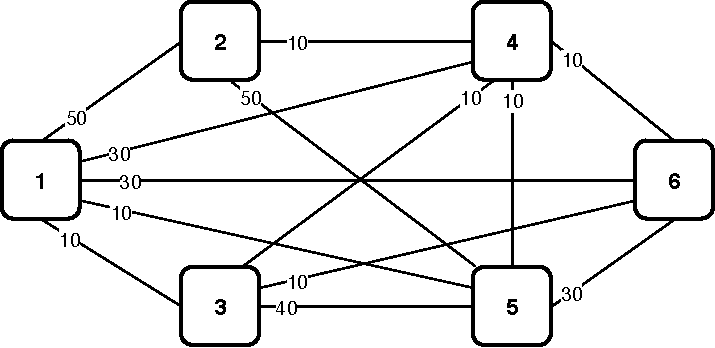
\includegraphics[width=12cm]{sdf/ilp/transparent_survivability/figures/logical_topology_ODU0_medium}
\caption{ODU0 logical topology defined by the ODU0 traffic matrix.}
\label{logical2_ODU0_medium}
\end{figure}

\begin{figure}[h!]
\centering
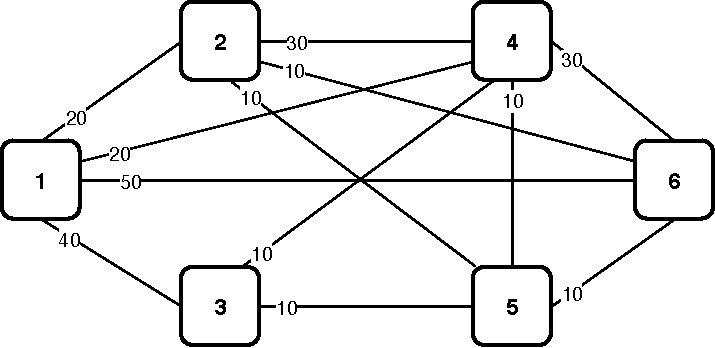
\includegraphics[width=12cm]{sdf/ilp/transparent_survivability/figures/logical_topology_ODU1_medium}
\caption{ODU1 logical topology defined by the ODU1 traffic matrix.}
\label{logical2_ODU1_medium}
\end{figure}

\begin{figure}[h!]
\centering
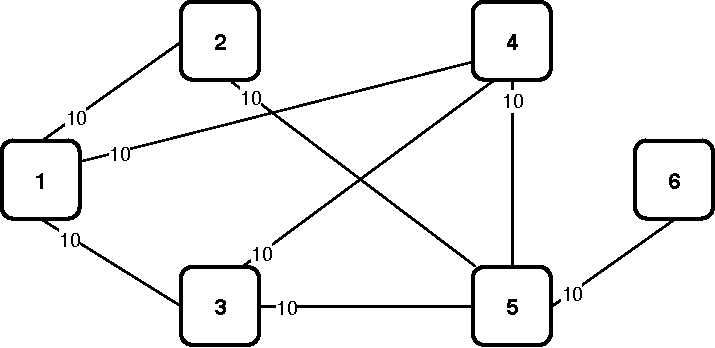
\includegraphics[width=12cm]{sdf/ilp/transparent_survivability/figures/logical_topology_ODU2_medium}
\caption{ODU2 logical topology defined by the ODU2 traffic matrix.}
\label{logical2_ODU2_medium}
\end{figure}

\begin{figure}[h!]
\centering
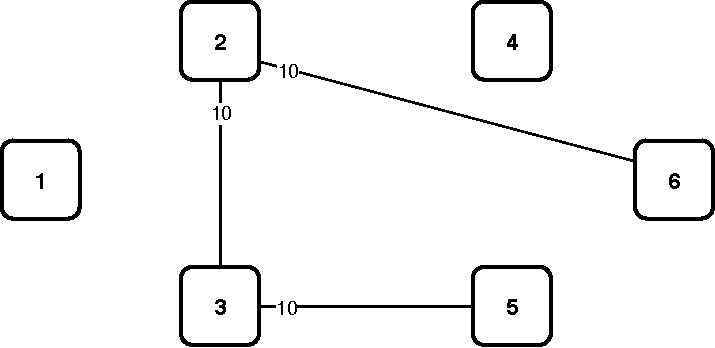
\includegraphics[width=12cm]{sdf/ilp/transparent_survivability/figures/logical_topology_ODU3_medium}
\caption{ODU3 logical topology defined by the ODU3 traffic matrix.}
\label{logical2_ODU3_medium}
\end{figure}

\begin{figure}[h!]
\centering
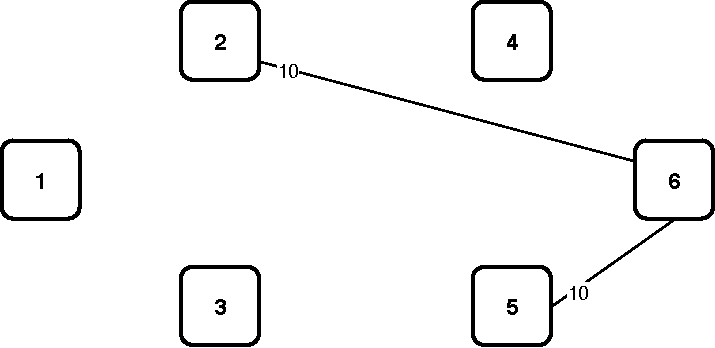
\includegraphics[width=12cm]{sdf/ilp/transparent_survivability/figures/logical_topology_ODU4_medium}
\caption{ODU4 logical topology defined by the ODU4 traffic matrix.}
\label{logical2_ODU4_medium}
\end{figure}

\begin{figure}[h!]
\centering
\includegraphics[width=12cm]{sdf/ilp/transparent_survivability/figures/physical_topology}
\caption{Physical topology after dimensioning.}
\label{physical2_medium}
\end{figure}
\newpage
\begin{figure}[h!]
\centering
\includegraphics[width=11cm]{sdf/ilp/transparent_survivability/figures/optical_topology_medium}
\caption{Optical topology after dimensioning.}
\label{optical2_medium}
\end{figure}

In table \ref{link_transp_surv_ref_medium} we can see the number of optical channels calculated using \ref{Capex_Link} and \ref{ILPOpaque_CAPEX} and the number of amplifiers for each link calculated using \ref{Capex_amplifiers}.

\begin{table}[h!]
\centering
\begin{tabular}{|| c | c | c ||}
 \hline
 \multicolumn{3}{|| c ||}{Information regarding links} \\
 \hline
 \hline
 Bidirectional Link & Optical Channels & Amplifiers\\
 \hline
 Node 1 <-> Node 2 & 7 & 4 \\
 Node 1 <-> Node 3 & 4 & 6 \\
 Node 2 <-> Node 3 & 8 & 0 \\
 Node 2 <-> Node 4 & 22 & 6 \\
 Node 3 <-> Node 5 & 10 & 8 \\
 Node 4 <-> Node 5 & 2 & 1 \\
 Node 4 <-> Node 6 & 18 & 7 \\
 Node 5 <-> Node 6 & 13 & 3 \\
 \hline
\end{tabular}
\caption{Table with information regarding links for transparent mode.}
\label{link_transp_surv_ref_medium}
\end{table}

In table \ref{node_transp_surv_ref_medium} we can see the number of line ports and add ports using \ref{OXC_poxc_transparent} the number of long-reach transponders using \ref{EXC_pexc2_transparent} and the number of tributary ports using \ref{EXC_pexc1_transparent}.

\begin{table}[h!]
\centering
\begin{tabular}{|| c | c | c | c | c | c ||}
 \hline
 \multicolumn{6}{|| c ||}{Information regarding nodes} \\
 \hline
 \hline
 \multicolumn{2}{|| c |}{ } & \multicolumn{2}{ c |}{Electrical part} & \multicolumn{2}{ c ||}{Optical part} \\
 \hline
 Node & Resulting Nodal Degree & Tributary Ports & LR Transponders & Add Ports & Line Ports\\
 \hline
 1 & 2 & 290 & 11 & 11 & 11 \\
 2 & 3 & 230 & 25 & 25 & 37 \\
 3 & 3 & 180 & 16 & 16 & 22 \\
 4 & 3 & 200 & 8 & 8 & 42 \\
 5 & 3 & 240 & 23 & 23 & 25 \\
 6 & 2 & 220 & 31 & 31 & 31 \\
\hline
\end{tabular}
\caption{Table with information regarding nodes for transparent mode.}
\label{node_transp_surv_ref_medium}
\end{table}

\newpage
Through the information obtained previously on the nodes we can now create tables with detailed information about each node. In each table mentioned below we can see how many ports are connected to a given node and its bit rate (in relation to the line ports and the add ports) and how many ports are assigned to each different bit rate (in relation to the tributary ports).\\

\begin{table}[h!]
\centering
\begin{tabular}{|| c | c | c ||}
 \hline
 \multicolumn{3}{|| c ||}{Detailed description of Node 1} \\
 \hline
 \hline
 Electrical part & Number of total demands & Bit rate \\ \hline
\multirow{3}{*}{290 tributary ports} & 130 & ODU0 \\
 & 130 & ODU1 \\
 & 30 & ODU2 \\
 \hline
  & Node<--Optical Channels-->Node & Bit rate \\ \hline
 \multirow{5}{*}{11 LR Transponders} & 1  <---- 3 ---->  2 & \multirow{5}{*}{100 Gbits/s} \\
  & 1  <---- 3 ---->  3 & \\
  & 1  <---- 2 ---->  4 & \\
  & 1  <---- 1 ---->  5 & \\
  & 1  <---- 2 ---->  6 & \\
 \hline
 \hline
 Optical part & Node<--Optical Channels-->Node & Bit rate \\
 \hline
 \multirow{5}{*}{11 add ports} & 1  <---- 3 ---->  2 & \multirow{10}{*}{100 Gbits/s} \\
  & 1  <---- 3 ---->  3 & \\
  & 1  <---- 2 ---->  4 & \\
  & 1  <---- 1 ---->  5 & \\
  & 1  <---- 2 ---->  6 & \\ \cline{1-2}
 \multirow{5}{*}{11 line ports} & 1  <---- 3 ---->  2 & \\
  & 1  <---- 3 ---->  3 & \\
  & 1  <---- 2 ---->  4 & \\
  & 1  <---- 1 ---->  5 & \\
  & 1  <---- 2 ---->  6 & \\
\hline
\end{tabular}
\caption{Table with detailed description of node 1. The number of demands is distributed to the various destination nodes, this distribution can be observed in section \ref{medium_traffic_scenario} . Regarding the number of line ports when this node is equal to the source, it means that add ports are used, otherwise it means that through ports are used.  In this node as we can see there are no through ports.}
\end{table}

\newpage
\begin{table}[h!]
\centering
\begin{tabular}{|| c | c | c ||}
 \hline
 \multicolumn{3}{|| c ||}{Detailed description of Node 2} \\
 \hline
 \hline
 Electrical part & Number of total demands & Bit rate \\ \hline
\multirow{5}{*}{230 tributary ports} & 110 & ODU0 \\
 & 70 & ODU1 \\
 & 20 & ODU2 \\
 & 20 & ODU3 \\
 & 10 & ODU4 \\
 \hline
  & Node<--Optical Channels-->Node & Bit rate \\
 \hline
 \multirow{5}{*}{25 LR Transponders} & 2  <---- 3 ---->  1 & \multirow{5}{*}{100 Gbits/s} \\
  & 2  <---- 4 ---->  3 & \\
  & 2  <---- 1 ---->  4 & \\
  & 2  <---- 2 ---->  5 & \\
  & 2  <---- 15 ---->  6 & \\
 \hline
 \hline
 Optical part & Node<--Optical Channels-->Node & Bit rate \\
 \hline
 \multirow{5}{*}{25 add ports} & 2  <---- 3 ---->  1 & \multirow{13}{*}{100 Gbits/s} \\
  & 2  <---- 4 ---->  3 & \\
  & 2  <---- 1 ---->  4 & \\
  & 2  <---- 2 ---->  5 & \\
  & 2  <---- 15 ---->  6 & \\ \cline{1-2}
 \multirow{8}{*}{37 line ports} & 2  <---- 3 ---->  1 & \\
  & 2  <---- 4 ---->  3 & \\
  & 2  <---- 1 ---->  4 & \\
  & 2  <---- 2 ---->  5 & \\
  & 2  <---- 15 ---->  6 & \\
  & 1  <---- 2 ---->  4 & \\
  & 1  <---- 2 ---->  6 & \\
  & 3  <---- 2 ---->  4 & \\
\hline
\end{tabular}
\caption{Table with detailed description of node 2. The number of demands is distributed to the various destination nodes, this distribution can be observed in section \ref{medium_traffic_scenario} . Regarding the number of line ports when this node is equal to the source, it means that add ports are used, otherwise it means that through ports are used. In the latter the number of ports is double the number of optical channels.}
\end{table}

\newpage
\begin{table}[h!]
\centering
\begin{tabular}{|| c | c | c ||}
 \hline
 \multicolumn{3}{|| c ||}{Detailed description of Node 3} \\
 \hline
 \hline
 Electrical part & Number of total demands & Bit rate \\ \hline
\multirow{4}{*}{180 tributary ports} & 70 & ODU0 \\
 & 60 & ODU1\\
 & 30 & ODU2\\
 & 20 & ODU3\\
 \hline
  & Node<--Optical Channels-->Node & Bit rate \\
 \hline
 \multirow{5}{*}{16 LR Transponders} & 3  <---- 3 ---->  1 & \multirow{5}{*}{100 Gbits/s} \\
  & 3  <---- 4 ---->  2 & \\
  & 3  <---- 2 ---->  4 & \\
  & 3  <---- 6 ---->  5 & \\
  & 3  <---- 1 ---->  6 & \\
 \hline
 \hline
 Optical part & Node<--Optical Channels-->Node & Bit rate \\
 \hline
 \multirow{5}{*}{16 add ports} & 3  <---- 3 ---->  1 & \multirow{12}{*}{100 Gbits/s}  \\
  & 3  <---- 4 ---->  2 & \\
  & 3  <---- 2 ---->  4 & \\
  & 3  <---- 6 ---->  5 & \\
  & 3  <---- 1 ---->  6 & \\ \cline{1-2}
 \multirow{7}{*}{22 line ports} & 3  <---- 3 ---->  1 & \\
  & 3  <---- 4 ---->  2 & \\
  & 3  <---- 2 ---->  4 & \\
  & 3  <---- 6 ---->  5 & \\
  & 3  <---- 1 ---->  6 & \\
  & 1  <---- 1 ---->  5 & \\
  & 2  <---- 2 ---->  5 & \\
\hline
\end{tabular}
\caption{Table with detailed description of node 3. The number of demands is distributed to the various destination nodes, this distribution can be observed in section \ref{medium_traffic_scenario} . Regarding the number of line ports when this node is equal to the source, it means that add ports are used, otherwise it means that through ports are used. In the latter the number of ports is double the number of optical channels.}
\end{table}

\newpage
\begin{table}[h!]
\centering
\begin{tabular}{|| c | c | c ||}
 \hline
 \multicolumn{3}{|| c ||}{Detailed description of Node 4} \\
 \hline
 \hline
 Electrical part & Number of total demands & Bit rate \\ \hline
\multirow{3}{*}{200 tributary ports} & 70 & ODU0 \\
 & 100 & ODU1 \\
 & 30 & ODU2 \\
 \hline
  & Node<--Optical Channels-->Node & Bit rate \\
 \hline
 \multirow{5}{*}{8 add ports} & 4  <---- 2 ---->  1 & \multirow{5}{*}{100 Gbits/s} \\
  & 4  <---- 1 ---->  2 & \\
  & 4  <---- 2 ---->  3 & \\
  & 4  <---- 2 ---->  5 & \\
  & 4  <---- 1 ---->  6 & \\
 \hline
 Optical part & Node<--Optical Channels-->Node & Bit rate \\
 \hline
 \multirow{5}{*}{8 add ports} & 4  <---- 2 ---->  1 & \multirow{12}{*}{100 Gbits/s} \\
  & 4  <---- 1 ---->  2 & \\
  & 4  <---- 2 ---->  3 & \\
  & 4  <---- 2 ---->  5 & \\
  & 4  <---- 1 ---->  6 & \\ \cline{1-2}
 \multirow{7}{*}{42 line ports} & 4  <---- 2 ---->  1 & \\
  & 4  <---- 1 ---->  2 & \\
  & 4  <---- 2 ---->  3 & \\
  & 4  <---- 2 ---->  5 & \\
  & 4  <---- 1 ---->  6 & \\
  & 1  <---- 2 ---->  6 & \\
  & 2  <---- 15 ---->  6 & \\
\hline
\end{tabular}
\caption{Table with detailed description of node 4. The number of demands is distributed to the various destination nodes, this distribution can be observed in section \ref{medium_traffic_scenario} . Regarding the number of line ports when this node is equal to the source, it means that add ports are used, otherwise it means that through ports are used. In the latter the number of ports is double the number of optical channels.}
\end{table}

\newpage
\begin{table}[h!]
\centering
\begin{tabular}{|| c | c | c ||}
 \hline
 \multicolumn{3}{|| c ||}{Detailed description of Node 5} \\
 \hline
 \hline
 Electrical part & Number of total demands & Bit rate \\ \hline
\multirow{5}{*}{240 tributary ports} & 140 & ODU0 \\
 & 40 & ODU1 \\
 & 40 & ODU2 \\
 & 10 & ODU3 \\
 & 10 & ODU4 \\
 \hline
  & Node<--Optical Channels-->Node & Bit rate \\
 \hline
 \multirow{5}{*}{23 LR Transponders} & 5  <---- 1 ---->  1 & \multirow{5}{*}{100 Gbits/s}\\
  & 5  <---- 2 ---->  2 & \\
  & 5  <---- 6 ---->  3 & \\
  & 5  <---- 2 ---->  4 & \\
  & 5  <---- 12 ---->  6 & \\
 \hline
 \hline
 Optical part & Node<--Optical Channels-->Node & Bit rate \\
 \hline
 \multirow{5}{*}{23 add ports} & 5  <---- 1 ---->  1 & \multirow{11}{*}{100 Gbits/s} \\
  & 5  <---- 2 ---->  2 & \\
  & 5  <---- 6 ---->  3 & \\
  & 5  <---- 2 ---->  4 & \\
  & 5  <---- 12 ---->  6 & \\ \cline{1-2}
 \multirow{6}{*}{25 line ports} & 5  <---- 1 ---->  1 & \\
  & 5  <---- 2 ---->  2 & \\
  & 5  <---- 6 ---->  3 & \\
  & 5  <---- 2 ---->  4 & \\
  & 5  <---- 12 ---->  6 & \\
  & 3  <---- 1 ---->  6 & \\
\hline
\end{tabular}
\caption{Table with detailed description of node 5. The number of demands is distributed to the various destination nodes, this distribution can be observed in section \ref{medium_traffic_scenario} . Regarding the number of line ports when this node is equal to the source, it means that add ports are used, otherwise it means that through ports are used. In the latter the number of ports is double the number of optical channels.}
\end{table}

\newpage
\begin{table}[h!]
\centering
\begin{tabular}{|| c | c | c ||}
 \hline
 \multicolumn{3}{|| c ||}{Detailed description of Node 6} \\
 \hline
 \hline
 Electrical part & Number of total demands & Bit rate \\ \hline
\multirow{5}{*}{220 tributary ports} & 80 & ODU0 \\
 & 100 & ODU1 \\
 & 10 & ODU2 \\
 & 10 & ODU3 \\
 & 20 & ODU4 \\
 \hline
  & Node<--Optical Channels-->Node & Bit rate \\
 \hline
 \multirow{5}{*}{31 LR Transponders} & 6  <---- 2 ---->  1 & \multirow{5}{*}{100 Gbits/s} \\
  & 6  <---- 15 ---->  2 & \\
  & 6  <---- 1 ---->  3 & \\
  & 6  <---- 1 ---->  4 & \\
  & 6  <---- 12 ---->  5 & \\
 \hline
 \hline
 Optical part & Node<--Optical Channels-->Node & Bit rate \\
 \hline
 \multirow{5}{*}{31 add ports} & 6  <---- 2 ---->  1 & \multirow{10}{*}{100 Gbits/s} \\
  & 6  <---- 15 ---->  2 & \\
  & 6  <---- 1 ---->  3 & \\
  & 6  <---- 1 ---->  4 & \\
  & 6  <---- 12 ---->  5 & \\ \cline{1-2}
 \multirow{3}{*}{31 line ports} & 6  <---- 2 ---->  1 & \\
  & 6  <---- 15 ---->  2 & \\
  & 6  <---- 1 ---->  3 & \\
  & 6  <---- 1 ---->  4 & \\
  & 6  <---- 12 ---->  5 & \\
\hline
\end{tabular}
\caption{Table with detailed description of node 6. The number of demands is distributed to the various destination nodes, this distribution can be observed in section \ref{medium_traffic_scenario} . Regarding the number of line ports when this node is equal to the source, it means that add ports are used, otherwise it means that through ports are used.  In this node as we can see there are no through ports.}
\end{table}

\vspace{17pt}
Now, in next page, let's focus on the routing information in table \ref{path_transp_surv_ref_medium}. These paths are bidirectional so the path from one node to another is the same path in the opposite direction.\\
\newpage
\begin{table}[h!]
\centering
\begin{tabular}{|| c | c | c ||}
 \hline
 \multicolumn{3}{|| c ||}{Routing} \\
 \hline
 \hline
 o & d & Links \\
 \hline
 1 & 2 & \{(1,2)\} \\ \hline
 1 & 3 & \{(1,3)\} \\ \hline
 1 & 4 & \{(1,2),(2,4)\}\\ \hline
 1 & 5 & \{(1,3),(3,5)\}\\ \hline
 1 & 6 & \{(1,2),(2,4),(4,6)\}\\ \hline
 2 & 3 & \{(2,3)\}\\ \hline
 2 & 4 & \{(2,4)\}\\ \hline
 2 & 5 & \{(2,3),(3,5)\}\\ \hline
 2 & 6 & \{(2,4),(4,6)\}\\ \hline
 3 & 4 & \{(3,2),(2,4)\}\\ \hline
 3 & 5 & \{(3,5)\}\\ \hline
 3 & 6 & \{(3,5),(5,6)\}\\ \hline
 4 & 5 & \{(4,5)\}\\ \hline
 4 & 6 & \{(4,6)\}\\ \hline
 5 & 6 & \{(5,6)\}\\
 \hline
\end{tabular}
\caption{Table with description of routing}
\label{path_transp_surv_ref_medium}
\end{table}

Finally and most importantly through table \ref{scripttransp_surv_ref_medium} we can see the CAPEX result for this model. This value is obtained using equation \ref{ILPOpaque_CAPEX} and all of the constraints mentioned above. In table \ref{formulas_transp} mentioned in previous scenario we can see how all the values were calculated.

\begin{table}[h!]
\centering
\begin{tabular}{|| c | c | c | c | c | c | c ||}
 \hline
 \multicolumn{7}{|| c ||}{CAPEX of the Network} \\
 \hline
 \hline
 \multicolumn{3}{|| c |}{ } & Quantity & Unit Price & Cost & Total \\
 \hline
 \multirow{3}{*}{Link Cost} & \multicolumn{2}{ c |}{OLTs} & 16 & 15 000 \euro & 240 000 \euro & \multirow{3}{*}{84 520 000 \euro} \\ \cline{2-6}
 & \multicolumn{2}{ c |}{100 Gbits/s Transceivers} & 168 & 5 000 \euro/Gbit/s & 84 000 000 \euro & \\ \cline{2-6}
 & \multicolumn{2}{ c |}{Amplifiers} & 70 & 4 000 \euro & 280 000 \euro & \\
 \hline
 \multirow{10}{*}{Node Cost} & \multirow{7}{*}{Electrical} & EXCs & 6 & 10 000 \euro & 60 000 \euro & \multirow{10}{*}{12 310 900 \euro} \\ \cline{3-6}
 & & ODU0 Ports & 600 & 10 \euro/port & 6 000 \euro & \\ \cline{3-6}
 & & ODU1 Ports & 500 & 15 \euro/port & 7 500 \euro & \\ \cline{3-6}
 & & ODU2 Ports & 160 & 30 \euro/port & 4 800 \euro & \\ \cline{3-6}
 & & ODU3 Ports & 60 & 60 \euro/port & 3 600 \euro & \\ \cline{3-6}
 & & ODU4 Ports & 40 & 100 \euro/port & 4 000 \euro & \\ \cline{3-6}
 & &Transponders& 114 & 100 000 \euro/port & 11 400 000 \euro & \\ \cline{2-6}
 & \multirow{3}{*}{Optical} & OXCs & 6 & 20 000 \euro & 120 000 \euro & \\ \cline{3-6}
 & & Line Ports & 168 & 2 500 \euro/port & 420 000 \euro & \\ \cline{3-6}
 & & Add Ports & 114 & 2 500 \euro/port & 285 000 \euro & \\
 \hline
 \multicolumn{6}{|| c |}{Total Network Cost} &96 830 900 \euro \\
\hline
\end{tabular}
\caption{Table with detailed description of CAPEX}
\label{scripttransp_surv_ref_medium}
\end{table}

\newpage
\textbf{High Traffic Scenario:}\\

In this scenario we have to take into account the traffic calculated in \ref{high_traffic_scenario}. In a first phase we will show the various existing topologies of the network. The first are the allowed topologies, physical and optical topology, the second are the logical topology for all ODUs and finally the resulting physical and optical topology.\\

\begin{figure}[h!]
\centering
\includegraphics[width=12cm]{sdf/ilp/transparent_survivability/figures/allowed_physical_topology}
\caption{Allowed physical topology. The allowed physical topology is defined by the duct and sites in the field. It is assumed that each duct supports up to 1 bidirectional transmission system and each site supports up to 1 node.}
\label{allowed2_physical_high}
\end{figure}

\vspace{11pt}
\begin{figure}[h!]
\centering
\includegraphics[width=12cm]{sdf/ilp/transparent_survivability/figures/allowed_optical_topology}
\caption{Allowed optical topology. The allowed optical topology is defined by the transport mode (transparent transport mode in this case). It is assumed that each connections between demands supports up to 100 lightpaths.}
\label{allowed2_optical_high}
\end{figure}

\newpage
\begin{figure}[h!]
\centering
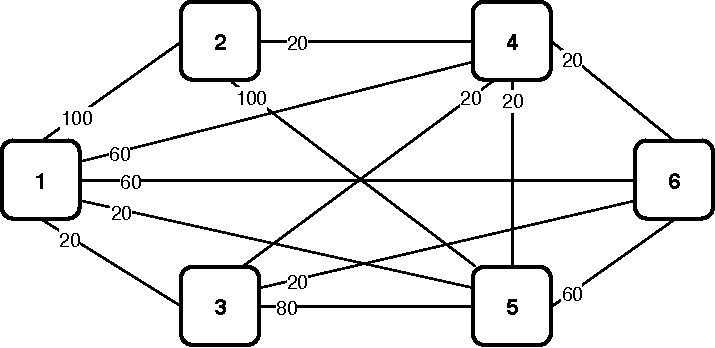
\includegraphics[width=12cm]{sdf/ilp/transparent_survivability/figures/logical_topology_ODU0_high}
\caption{ODU0 logical topology defined by the ODU0 traffic matrix.}
\label{logical2_ODU0_high}
\end{figure}

\begin{figure}[h!]
\centering
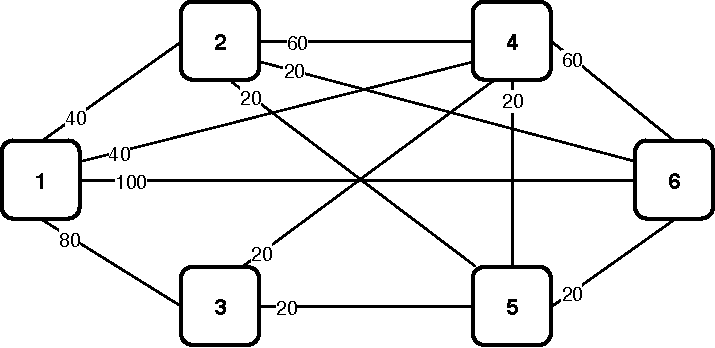
\includegraphics[width=12cm]{sdf/ilp/transparent_survivability/figures/logical_topology_ODU1_high}
\caption{ODU1 logical topology defined by the ODU1 traffic matrix.}
\label{logical2_ODU1_high}
\end{figure}

\begin{figure}[h!]
\centering
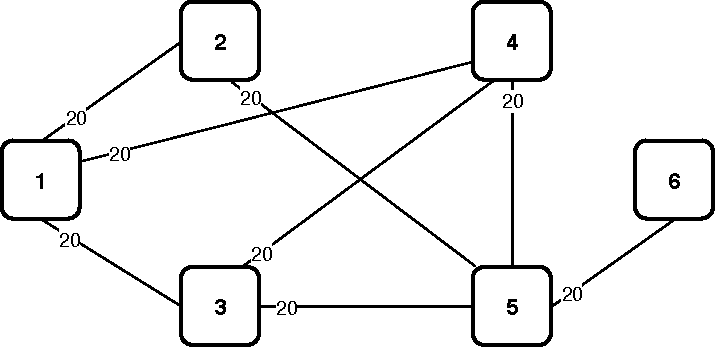
\includegraphics[width=12cm]{sdf/ilp/transparent_survivability/figures/logical_topology_ODU2_high}
\caption{ODU2 logical topology defined by the ODU2 traffic matrix.}
\label{logical2_ODU2_high}
\end{figure}

\begin{figure}[h!]
\centering
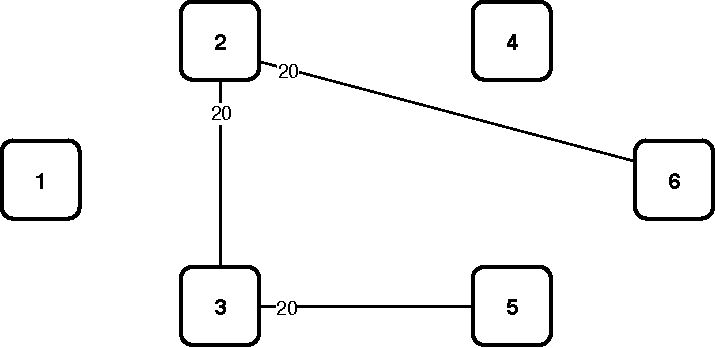
\includegraphics[width=12cm]{sdf/ilp/transparent_survivability/figures/logical_topology_ODU3_high}
\caption{ODU3 logical topology defined by the ODU3 traffic matrix.}
\label{logical2_ODU3_high}
\end{figure}

\begin{figure}[h!]
\centering
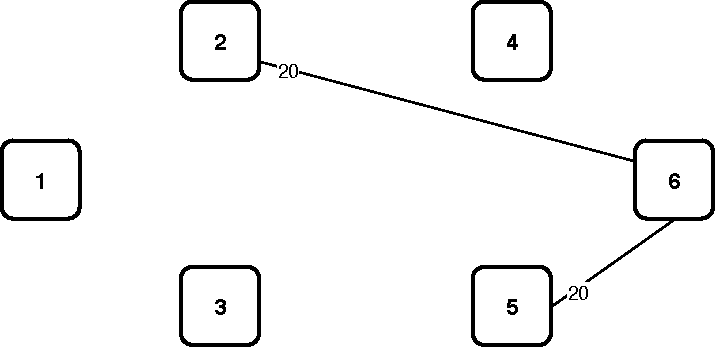
\includegraphics[width=12cm]{sdf/ilp/transparent_survivability/figures/logical_topology_ODU4_high}
\caption{ODU4 logical topology defined by the ODU4 traffic matrix.}
\label{logical2_ODU4_high}
\end{figure}

\begin{figure}[h!]
\centering
\includegraphics[width=12cm]{sdf/ilp/transparent_survivability/figures/physical_topology}
\caption{Physical topology after dimensioning.}
\label{physical2_high}
\end{figure}

\newpage
\begin{figure}[h!]
\centering
\includegraphics[width=11cm]{sdf/ilp/transparent_survivability/figures/optical_topology_high}
\caption{Optical topology after dimensioning.}
\label{optical2_high}
\end{figure}

In table \ref{link_transp_surv_ref_high} we can see the number of optical channels calculated using \ref{Capex_Link} and \ref{ILPOpaque_CAPEX} and the number of amplifiers for each link calculated using \ref{Capex_amplifiers}.

\begin{table}[h!]
\centering
\begin{tabular}{|| c | c | c ||}
 \hline
 \multicolumn{3}{|| c ||}{Information regarding links} \\
 \hline
 \hline
 Bidirectional Link & Optical Channels & Amplifiers\\
 \hline
 Node 1 <-> Node 2 & 13 & 4 \\
 Node 1 <-> Node 3 & 6 & 6 \\
 Node 2 <-> Node 3 & 15 & 0 \\
 Node 2 <-> Node 4 & 42 & 6 \\
 Node 3 <-> Node 5 & 18 & 8 \\
 Node 4 <-> Node 5 & 3 & 1 \\
 Node 4 <-> Node 6 & 35 & 7 \\
 Node 5 <-> Node 6 & 25 & 3 \\
 \hline
\end{tabular}
\caption{Table with information regarding links for transparent mode.}
\label{link_transp_surv_ref_high}
\end{table}

In table \ref{node_transp_surv_ref_high} we can see the number of line ports and add ports using \ref{OXC_poxc_transparent} the number of long-reach transponders using \ref{EXC_pexc2_transparent} and the number of tributary ports using \ref{EXC_pexc1_transparent}.

\begin{table}[h!]
\centering
\begin{tabular}{|| c | c | c | c | c | c ||}
 \hline
 \multicolumn{6}{|| c ||}{Information regarding nodes} \\
 \hline
 \hline
 \multicolumn{2}{|| c |}{ } & \multicolumn{2}{ c |}{Electrical part} & \multicolumn{2}{ c ||}{Optical part} \\
 \hline
 Node & Resulting Nodal Degree & Tributary Ports & LR Transponders & Add Ports & Line Ports\\
 \hline
 1 & 2 & 580 & 19 & 19 & 19 \\
 2 & 3 & 460 & 48 & 48 & 70 \\
 3 & 3 & 360 & 29 & 29 & 39 \\
 4 & 3 & 400 & 14 & 14 & 80 \\
 5 & 3 & 480 & 44 & 44 & 46 \\
 6 & 2 & 440 & 60 & 60 & 60 \\
\hline
\end{tabular}
\caption{Table with information regarding nodes for transparent mode.}
\label{node_transp_surv_ref_high}
\end{table}

\newpage
Through the information obtained previously on the nodes we can now create tables with detailed information about each node. In each table mentioned below we can see how many ports are connected to a given node and its bit rate (in relation to the line ports and the add ports) and how many ports are assigned to each different bit rate (in relation to the tributary ports).\\

\begin{table}[h!]
\centering
\begin{tabular}{|| c | c | c ||}
 \hline
 \multicolumn{3}{|| c ||}{Detailed description of Node 1} \\
 \hline
 \hline
 Electrical part & Number of total demands & Bit rate \\ \hline
\multirow{3}{*}{580 tributary ports} & 260 & ODU0 \\
 & 260 & ODU1 \\
 & 60 & ODU2 \\
 \hline
  & Node<--Optical Channels-->Node & Bit rate \\
 \hline
 \multirow{5}{*}{19 LR Transponders} & 1  <---- 5 ---->  2 & \multirow{5}{*}{100 Gbits/s} \\
  & 1  <---- 5 ---->  3 & \\
  & 1  <---- 4 ---->  4 & \\
  & 1  <---- 1 ---->  5 & \\
  & 1  <---- 4 ---->  6 & \\
 \hline
 \hline
 Optical part & Node<--Optical Channels-->Node & Bit rate \\
 \hline
 \multirow{5}{*}{19 add ports} & 1  <---- 5 ---->  2 & \multirow{10}{*}{100 Gbits/s} \\
  & 1  <---- 5 ---->  3 & \\
  & 1  <---- 4 ---->  4 & \\
  & 1  <---- 1 ---->  5 & \\
  & 1  <---- 4 ---->  6 & \\ \cline{1-2}
 \multirow{5}{*}{19 line ports} & 1  <---- 5 ---->  2 & \\
  & 1  <---- 5 ---->  3 & \\
  & 1  <---- 4 ---->  4 & \\
  & 1  <---- 1 ---->  5 & \\
  & 1  <---- 4 ---->  6 & \\
\hline
\end{tabular}
\caption{Table with detailed description of node 1. The number of demands is distributed to the various destination nodes, this distribution can be observed in section \ref{high_traffic_scenario}. Regarding the number of line ports when this node is equal to the source, it means that add ports are used, otherwise it means that through ports are used. In this node as we can see there are no through ports.}
\end{table}

\newpage
\begin{table}[h!]
\centering
\begin{tabular}{|| c | c | c ||}
 \hline
 \multicolumn{3}{|| c ||}{Detailed description of Node 2} \\
 \hline
 \hline
 Electrical part & Number of total demands & Bit rate \\ \hline
\multirow{5}{*}{460 tributary ports} & 220 & ODU0 \\
 & 140 & ODU1 \\
 & 40 & ODU2 \\
 & 40 & ODU3 \\
 & 20 & ODU4 \\
 \hline
  & Node<--Optical Channels-->Node & Bit rate \\
 \hline
 \multirow{5}{*}{48 LR Transponders} & 2  <---- 5 ---->  1 & \multirow{5}{*}{100 Gbits/s} \\
  & 2  <---- 8 ---->  3 & \\
  & 2  <---- 2 ---->  4 & \\
  & 2  <---- 4 ---->  5 & \\
  & 2  <---- 29 ---->  6 & \\
 \hline
 \hline
 Optical part & Node<--Optical Channels-->Node & Bit rate \\
 \hline
 \multirow{5}{*}{48 add ports} & 2  <---- 5 ---->  1 & \multirow{13}{*}{100 Gbits/s} \\
  & 2  <---- 8 ---->  3 & \\
  & 2  <---- 2 ---->  4 & \\
  & 2  <---- 4 ---->  5 & \\
  & 2  <---- 29 ---->  6 & \\ \cline{1-2}
 \multirow{8}{*}{70 line ports} & 2  <---- 5 ---->  1 & \\
  & 2  <---- 8 ---->  3 & \\
  & 2  <---- 2 ---->  4 & \\
  & 2  <---- 4 ---->  5 & \\
  & 2  <---- 29 ---->  6 & \\
  & 1  <---- 4 ---->  4 & \\
  & 1  <---- 4 ---->  6 & \\
  & 3  <---- 3 ---->  4 & \\
\hline
\end{tabular}
\caption{Table with detailed description of node 2. The number of demands is distributed to the various destination nodes, this distribution can be observed in section \ref{high_traffic_scenario} . Regarding the number of line ports when this node is equal to the source, it means that add ports are used, otherwise it means that through ports are used. In the latter the number of ports is double the number of optical channels.}
\end{table}

\newpage
\begin{table}[h!]
\centering
\begin{tabular}{|| c | c | c ||}
 \hline
 \multicolumn{3}{|| c ||}{Detailed description of Node 3} \\
 \hline
 \hline
 Electrical part & Number of total demands & Bit rate \\ \hline
\multirow{4}{*}{360 tributary ports} & 140 & ODU0 \\
 & 120 & ODU1\\
 & 60 & ODU2\\
 & 40 & ODU3\\
 \hline
  & Node<--Optical Channels-->Node & Bit rate \\
 \hline
 \multirow{5}{*}{29 LR Transponders} & 3  <---- 5 ---->  1 & \multirow{5}{*}{100 Gbits/s} \\
  & 3  <---- 8 ---->  2 & \\
  & 3  <---- 3 ---->  4 & \\
  & 3  <---- 12 ---->  5 & \\
  & 3  <---- 1 ---->  6 & \\
 \hline
 \hline
 Optical part & Node<--Optical Channels-->Node & Bit rate \\
 \hline
 \multirow{5}{*}{29 add ports} & 3  <---- 5 ---->  1 & \multirow{12}{*}{100 Gbits/s} \\
  & 3  <---- 8 ---->  2 & \\
  & 3  <---- 3 ---->  4 & \\
  & 3  <---- 12 ---->  5 & \\
  & 3  <---- 1 ---->  6 & \\ \cline{1-2}
 \multirow{7}{*}{39 line ports} & 3  <---- 5 ---->  1 & \\
  & 3  <---- 8 ---->  2 & \\
  & 3  <---- 3 ---->  4 & \\
  & 3  <---- 12 ---->  5 & \\
  & 3  <---- 1 ---->  6 & \\
  & 1  <---- 1 ---->  5 & \\
  & 2  <---- 4 ---->  5 & \\
\hline
\end{tabular}
\caption{Table with detailed description of node 3. The number of demands is distributed to the various destination nodes, this distribution can be observed in section \ref{high_traffic_scenario} . Regarding the number of line ports when this node is equal to the source, it means that add ports are used, otherwise it means that through ports are used. In the latter the number of ports is double the number of optical channels.}
\end{table}

\newpage
\begin{table}[h!]
\centering
\begin{tabular}{|| c | c | c ||}
 \hline
 \multicolumn{3}{|| c ||}{Detailed description of Node 4} \\
 \hline
 \hline
 Electrical part & Number of total demands & Bit rate \\ \hline
\multirow{3}{*}{400 tributary ports} & 140 & ODU0 \\
 & 200 & ODU1 \\
 & 60 & ODU2 \\
 \hline
  & Node<--Optical Channels-->Node & Bit rate \\
 \hline
 \multirow{5}{*}{14 LR Transponders} & 4  <---- 4 ---->  1 & \multirow{5}{*}{100 Gbits/s} \\
  & 4  <---- 2 ---->  2 & \\
  & 4  <---- 3 ---->  3 & \\
  & 4  <---- 3 ---->  5 & \\
  & 4  <---- 2 ---->  6 & \\
 \hline
 \hline
 Optical part & Node<--Optical Channels-->Node & Bit rate \\
 \hline
 \multirow{5}{*}{14 add ports} & 4  <---- 4 ---->  1 & \multirow{12}{*}{100 Gbits/s} \\
  & 4  <---- 2 ---->  2 & \\
  & 4  <---- 3 ---->  3 & \\
  & 4  <---- 3 ---->  5 & \\
  & 4  <---- 2 ---->  6 & \\ \cline{1-2}
 \multirow{7}{*}{80 line ports} & 4  <---- 4 ---->  1 & \\
  & 4  <---- 2 ---->  2 & \\
  & 4  <---- 3 ---->  3 & \\
  & 4  <---- 3 ---->  5 & \\
  & 4  <---- 2 ---->  6 & \\
  & 1  <---- 4 ---->  6 & \\
  & 2  <---- 29 ---->  6 & \\
\hline
\end{tabular}
\caption{Table with detailed description of node 4. The number of demands is distributed to the various destination nodes, this distribution can be observed in section \ref{high_traffic_scenario} . Regarding the number of line ports when this node is equal to the source, it means that add ports are used, otherwise it means that through ports are used. In the latter the number of ports is double the number of optical channels.}
\end{table}

\newpage
\begin{table}[h!]
\centering
\begin{tabular}{|| c | c | c ||}
 \hline
 \multicolumn{3}{|| c ||}{Detailed description of Node 5} \\
 \hline
 \hline
 Electrical part & Number of total demands & Bit rate \\ \hline
\multirow{5}{*}{480 tributary ports} & 280 & ODU0 \\
 & 80 & ODU1 \\
 & 80 & ODU2 \\
 & 20 & ODU3 \\
 & 20 & ODU4 \\
 \hline
  & Node<--Optical Channels-->Node & Bit rate \\
 \hline
 \multirow{5}{*}{44 LR Transponders} & 5  <---- 1 ---->  1 & \multirow{5}{*}{100 Gbits/s} \\
  & 5  <---- 4 ---->  2 & \\
  & 5  <---- 12 ---->  3 & \\
  & 5  <---- 3 ---->  4 & \\
  & 5  <---- 24 ---->  6 & \\
 \hline
 \hline
 Optical part & Node<--Optical Channels-->Node & Bit rate \\
 \hline
 \multirow{5}{*}{44 add ports} & 5  <---- 1 ---->  1 & \multirow{11}{*}{100 Gbits/s} \\
  & 5  <---- 4 ---->  2 & \\
  & 5  <---- 12 ---->  3 & \\
  & 5  <---- 3 ---->  4 & \\
  & 5  <---- 24 ---->  6 & \\ \cline{1-2}
 \multirow{6}{*}{46 line ports} & 5  <---- 1 ---->  1 & \\
  & 5  <---- 4 ---->  2 & \\
  & 5  <---- 12 ---->  3 & \\
  & 5  <---- 3 ---->  4 & \\
  & 5  <---- 24 ---->  6 & \\
  & 3  <---- 1 ---->  6 & \\
\hline
\end{tabular}
\caption{Table with detailed description of node 5. The number of demands is distributed to the various destination nodes, this distribution can be observed in section \ref{high_traffic_scenario} . Regarding the number of line ports when this node is equal to the source, it means that add ports are used, otherwise it means that through ports are used. In the latter the number of ports is double the number of optical channels.}
\end{table}

\newpage
\begin{table}[h!]
\centering
\begin{tabular}{|| c | c | c ||}
 \hline
 \multicolumn{3}{|| c ||}{Detailed description of Node 6} \\
 \hline
 \hline
 Electrical part & Number of total demands & Bit rate \\ \hline
\multirow{5}{*}{440 tributary ports} & 160 & ODU0 \\
 & 200 & ODU1 \\
 & 20 & ODU2 \\
 & 20 & ODU3 \\
 & 40 & ODU4 \\
 \hline
  & Node<--Optical Channels-->Node & Bit rate \\
 \hline
 \multirow{5}{*}{60 LR Transponders} & 6  <---- 4 ---->  1 & \multirow{5}{*}{100 Gbits/s} \\
  & 6  <---- 29 ---->  2 & \\
  & 6  <---- 1 ---->  3 & \\
  & 6  <---- 2 ---->  4 & \\
  & 6  <---- 24 ---->  5 & \\
 \hline
 \hline
 Optical part & Node<--Optical Channels-->Node & Bit rate \\
 \hline
 \multirow{5}{*}{60 add ports} & 6  <---- 4 ---->  1 & \multirow{10}{*}{100 Gbits/s} \\
  & 6  <---- 29 ---->  2 & \\
  & 6  <---- 1 ---->  3 & \\
  & 6  <---- 2 ---->  4 & \\
  & 6  <---- 24 ---->  5 & \\ \cline{1-2}
 \multirow{5}{*}{60 line ports} & 6  <---- 4 ---->  1 & \\
  & 6  <---- 29 ---->  2 & \\
  & 6  <---- 1 ---->  3 & \\
  & 6  <---- 2 ---->  4 & \\
  & 6  <---- 24 ---->  5 & \\
\hline
\end{tabular}
\caption{Table with detailed description of node 6. The number of demands is distributed to the various destination nodes, this distribution can be observed in section \ref{high_traffic_scenario}. Regarding the number of line ports when this node is equal to the source, it means that add ports are used, otherwise it means that through ports are used. In this node as we can see there are no through ports.}
\end{table}

\vspace{17pt}
Now, in next page, let's focus on the routing information in table \ref{path_transp_surv_ref_high}. These paths are bidirectional so the path from one node to another is the same path in the opposite direction.\\
\newpage
\begin{table}[h!]
\centering
\begin{tabular}{|| c | c | c ||}
 \hline
 \multicolumn{3}{|| c ||}{Routing} \\
 \hline
 \hline
 o & d & Links \\
 \hline
 1 & 2 & \{(1,2)\} \\ \hline
 1 & 3 & \{(1,3)\} \\ \hline
 1 & 4 & \{(1,2),(2,4)\}\\ \hline
 1 & 5 & \{(1,3),(3,5)\}\\ \hline
 1 & 6 & \{(1,2),(2,4),(4,6)\}\\ \hline
 2 & 3 & \{(2,3)\}\\ \hline
 2 & 4 & \{(2,4)\}\\ \hline
 2 & 5 & \{(2,3),(3,5)\}\\ \hline
 2 & 6 & \{(2,4),(4,6)\}\\ \hline
 3 & 4 & \{(3,2),(2,4)\}\\ \hline
 3 & 5 & \{(3,5)\}\\ \hline
 3 & 6 & \{(3,5),(5,6)\}\\ \hline
 4 & 5 & \{(4,5)\}\\ \hline
 4 & 6 & \{(4,6)\}\\ \hline
 5 & 6 & \{(5,6)\}\\
 \hline
\end{tabular}
\caption{Table with description of routing}
\label{path_transp_surv_ref_high}
\end{table}

Finally and most importantly through table \ref{scripttransp_surv_ref_high} we can see the CAPEX result for this model. This value is obtained using equation \ref{ILPOpaque_CAPEX} and all of the constraints mentioned above. In table \ref{formulas_transp} mentioned in previous scenario we can see how all the values were calculated.

\begin{table}[h!]
\centering
\begin{tabular}{|| c | c | c | c | c | c | c ||}
 \hline
 \multicolumn{7}{|| c ||}{CAPEX of the Network} \\
 \hline
 \hline
 \multicolumn{3}{|| c |}{ } & Quantity & Unit Price & Cost & Total \\
 \hline
 \multirow{3}{*}{Link Cost} & \multicolumn{2}{ c |}{OLTs} & 16 & 15 000 \euro & 240 000 \euro & \multirow{3}{*}{157 520 000 \euro} \\ \cline{2-6}
 & \multicolumn{2}{ c |}{100 Gbits/s Transceivers} & 314 & 5 000 \euro/Gbit/s & 157 000 000 \euro & \\ \cline{2-6}
 & \multicolumn{2}{ c |}{Amplifiers} & 70 & 4 000 \euro & 280 000 \euro & \\
 \hline
 \multirow{10}{*}{Node Cost} & \multirow{7}{*}{Electrical} & EXCs & 6 & 10 000 \euro & 60 000 \euro & \multirow{10}{*}{22 951 800 \euro} \\ \cline{3-6}
 & & ODU0 Ports & 1 200 & 10 \euro/port & 12 000 \euro & \\ \cline{3-6}
 & & ODU1 Ports & 1 000 & 15 \euro/port & 15 000 \euro & \\ \cline{3-6}
 & & ODU2 Ports & 320 & 30 \euro/port & 9 600 \euro & \\ \cline{3-6}
 & & ODU3 Ports & 120 & 60 \euro/port & 7 200 \euro & \\ \cline{3-6}
 & & ODU4 Ports & 80 & 100 \euro/port & 8 000 \euro & \\ \cline{3-6}
 & &Transponders& 214 & 100 000 \euro/port & 21 400 000 \euro & \\ \cline{2-6}
 & \multirow{3}{*}{Optical} & OXCs & 6 & 20 000 \euro & 120 000 \euro & \\ \cline{3-6}
 & & Line Ports & 314 & 2 500 \euro/port & 785 000 \euro & \\ \cline{3-6}
 & & Add Ports & 214 & 2 500 \euro/port & 535 000 \euro & \\
 \hline
 \multicolumn{6}{|| c |}{Total Network Cost} & 180 471 800 \euro \\
\hline
\end{tabular}
\caption{Table with detailed description of CAPEX for this scenario.}
\label{scripttransp_surv_ref_high}
\end{table}

\newpage
\subsubsection{Conclusions}

Once we have obtained the results for all the scenarios we will now draw some conclusions about these results. For a better analysis of the results will be created the table \ref{table_comparative_transp_surv} with the number of line ports and add ports of the optical part, the tributary ports, the transponders and transceivers because they are important values for the cost of CAPEX, the cost of links, the cost of nodes and finally the cost of CAPEX.\\

\begin{table}[h!]
\centering
\begin{tabular}{| c | c | c | c |}
 \hline
  & Low Traffic & Medium Traffic  & High Traffic \\
 \hline\hline
 Traffic (Gbit/s) & 500 & 5 000 & 10 000 \\ \hline
 Number of Add ports & 34 & 114 & 214 \\ \hline
 Number of Line ports & 52 & 168 & 314 \\ \hline
 Number of Tributary ports & 136 & 1 360 & 2 720 \\ \hline
 Number of Transceivers & 52 & 168 & 314 \\ \hline
 Number of Transponders & 34 & 114 & 214 \\ \hline
 Link Cost & 26 520 000 \euro & 84 520 000 \euro & 157 520 000 \euro \\ \hline
 Node Cost & 3 797 590 \euro & 12 310 900 \euro & 22 951 800 \euro \\ \hline
 CAPEX & \textbf{30 317 590 \euro} & \textbf{96 830 900 \euro} & \textbf{180 471 800 \euro} \\ \hline
 CAPEX/Gbit/s & \textbf{60 635 \euro/Gbit/s} & \textbf{19 366 \euro/Gbit/s} & \textbf{18 047 \euro/Gbit/s}\\
 \hline
\end{tabular}
\caption{Table with the various CAPEX values obtained in the different traffic scenarios.}
\label{table_comparative_transp_surv}
\end{table}

Looking at the previous table we can make some comparisons between the several scenarios:

\begin{itemize}
    \item Comparing the low traffic scenario with the others, we can see that, despite having an increase of factor ten (average scenario) and factor twenty (high scenario), the same increase does not occur in the final cost (it is lower). This happens because the number of transceivers is smaller than expected (an medium scenario of 520 would be expected and a high scenario would be expected in 1040);
    \item Comparing the medium traffic scenario with the high traffic scenario, we can see that the factor increase is double and in the final cost this factor is very close but still lower. Again, this happens because the number of transceivers is smaller, but very close to what was expected (the high scenario would be expected at 336);
    \item Comparing the cost with the traffic, we see that, for the low traffic scenario, the cost per traffic is very high in relation to the other two. We can conclude that a low traffic scenario becomes more expensive than a high traffic scenario.
\end{itemize}


\vspace{13pt}
\subsubsection{Opens Issues}

The creation of this model for any scenario, started with some considerations and some open issues being:

\begin{itemize}
  \item Allow blocking.
  \subitem The presented model assume that the solution is possible or impossible, does not support a partial solution where some demands are not routed (are blocked).
  \item Allow multiple transmission system.
  \subitem The presented model for each link only supports one transmission system.
\end{itemize}


\clearpage

\subsection{Transparent with 1+1 Protection}\label{ILP_Transp_Protection}
\begin{tcolorbox}	
\begin{tabular}{p{2.75cm} p{0.2cm} p{10.5cm}} 	
\textbf{Student Name}  &:& Tiago Esteves    (October 03, 2017 - )\\
\textbf{Goal}          &:& Implement the ILP model for the transparent transport mode with 1 plus 1 protection.
\end{tabular}
\end{tcolorbox}
\vspace{11pt}

Here, in this case, we must take into account table \ref{description_transp}, previously mentioned, in order to better understand the objective function.\\

Before carrying out the description of the objective function we must take into account the following particularity of this mode of transport:
\begin{itemize}
  \item $N_{OXC,n}$ = 1, \quad $\forall$ n that process traffic
  \item $N_{EXC,n}$ = 1, \quad $\forall$ n that process traffic
\end{itemize}

\vspace{11pt}
The objective function of following the ILP is a minimization of the CAPEX through the equation \ref{Capex} where in this case for the cost of nodes we have in consideration the electric cost \ref{Capex_Node_EXC} and the optical cost \ref{Capex_Node_OXC}.
In this case the value of $P_{exc,c,n}$ is obtained by equation \ref{EXC_pexc1_transparentp} for short-reach and by the equation \ref{EXC_pexc2_transparentp} for long-reach and the value of $P_{oxc,n}$ is obtained by equation \ref{OXC_poxc_transparentp}.\\

The equation \ref{EXC_pexc1_transparentp} refers to the number of sort-reach ports of the electrical switch with bit-rate $c$ in node $n$, $P_{exc,c,n}$, i.e. the number of tributary ports with bit-rate $c$ in node $n$ which can be calculated as

\begin{equation}
P_{exc,c,n} = \sum_{d=1}^{N} D_{nd,c}
\label{EXC_pexc1_transparentp}
\end{equation}

\vspace{11pt}
\noindent
where $D_{nd,c}$ are the client demands between nodes $n$ and $d$ with bit rate $c$.\\

In this case there is the following particularity:

\begin{itemize}
  \item When $n$=$d$ the value of client demands is always zero, i.e, $D_{nn,c}=0$
\end{itemize}

\vspace{11pt}
As previously mentioned, the equation \ref{EXC_pexc2_transparentp} refers to the number of long-reach ports of the electrical switch with bit-rate -1 in node n, $P_{exc,-1,n}$, i.e. the number of add ports of node n which can be calculated as

\begin{equation}
P_{exc,-1,n} = \sum_{j=1}^{N} \lambda_{nj}
\label{EXC_pexc2_transparentp}
\end{equation}

\vspace{11pt}
\noindent
where $\lambda_{nj}$ is the number of optical channels between node $n$ and node $j$.\\

The equation \ref{OXC_poxc_transparentp} refers to the number of ports in optical switch in node n, $P_{oxc,n}$, i.e. the number of line ports and the number of adding ports of node n which can be calculated as

\begin{equation}
P_{oxc,n} = \sum_{j=1}^{N} f_{nj}^{od} + \sum_{j=1}^{N} \lambda_{nj}
\label{OXC_poxc_transparentp}
\end{equation}

\vspace{11pt}
\noindent
where $f_{nj}^{od}$ refers to the number of line ports for all demand pairs (od) and $\lambda_{nj}$ refers to the number of add ports.\\

The objective function, to be minimized, is the expression \ref{ILPOpaque_CAPEX}, i.e.,
\begin{equation*}
  minimize \qquad \Big\{ \quad C_C \quad \Big\}
\end{equation*}

$subject$ $to$
\begin{equation}
\sum_{c\in C} B\left(c\right) D_{odc} \leq \tau \lambda_{od} \qquad \qquad \qquad \qquad \qquad \qquad \qquad \qquad \qquad \qquad
\forall(o,d) : o < d
\label{ILPTransp0}
\end{equation}
\noindent
This restriction is considered grooming constraint and for this model the grooming can be done before routing since the traffic is aggregated just for demands between the same nodes, thus not depending on the routes. The variable  $\tau$ is always 100 Gbits/s.

\begin{equation}
\sum_{j\textbackslash \{o\}} f_{ij}^{od} = \lambda_{od} \qquad \qquad \qquad \qquad \qquad \qquad \qquad \qquad \qquad
\forall(o,d) : o < d, \forall i: i = o
\label{ILPTransp1}
\end{equation}
\noindent
This constraint are equal to the constraint \ref{ILPOpaque1_CAPEX} assuming that Z variable has the value of number of optical channels between this demand for all bidirectional links.

\begin{equation}
\sum_{j\textbackslash \{o\}} f_{ij}^{od} = \sum_{j\textbackslash \{d\}} f_{ji}^{od} \qquad \qquad \qquad \qquad \qquad \qquad \qquad \qquad
\forall(o,d) : o < d, \forall i: i \neq o,d
\label{ILPTransp2}
\end{equation}
\noindent
This constraint are equal to the constraint \ref{ILPOpaque2_CAPEX}.

\begin{equation}
\sum_{j\textbackslash \{d\}} f_{ji}^{od} = \lambda_{od}  \qquad \qquad \qquad \qquad \qquad \qquad \qquad \qquad \qquad
\forall(o,d) : o < d, \forall i: i = d
\label{ILPTransp3}
\end{equation}
\noindent
This constraint are equal to the constraint \ref{ILPOpaque3_CAPEX} assuming that Z variable has the value of number of optical channels between this demand for all bidirectional links.
\newpage
\begin{equation}
\sum_{j\textbackslash \{o\}} fp_{ij}^{od} = \lambda_{od} \qquad \qquad \qquad \qquad \qquad \qquad \qquad \qquad \qquad
\forall(o,d) : o < d, \forall i: i = o
\label{ILPTransp1p}
\end{equation}
\noindent
This are the protection flow conservation constraints and ensure that, for each $(o,d)$ pair, we route the number of optical channels units of flow from node $o$ to node $d$, the source node sends the number of optical channels units of flow.

\begin{equation}
\sum_{j\textbackslash \{o\}} fp_{ij}^{od} = \sum_{j\textbackslash \{d\}} fp_{ji}^{od} \qquad \qquad \qquad \qquad \qquad \qquad \qquad
\forall(o,d) : o < d, \forall i: i \neq o,d
\label{ILPTransp2p}
\end{equation}
\noindent
This constraint ensure that the remaining nodes, being neither origin or destination, the receive flow have to be send.

\begin{equation}
\sum_{j\textbackslash \{d\}} fp_{ji}^{od} = \lambda_{od} \qquad \qquad \qquad \qquad \qquad \qquad \qquad \qquad \qquad
\forall(o,d) : o < d, \forall i: i = d
\label{ILPTransp3p}
\end{equation}
\noindent
This are the usual flow conservation constraints and ensure that, for each $(o,d)$ pair, we route the number of optical channels units of flow from node $o$ to node $d$, the destination node has to receive those numbers of optical channels units of flow.

\begin{equation}
\sum_{o=1} \sum_{d=o+1} \left(f_{ij}^{od}  + fp_{ij}^{od}\right) \leq \lambda_{od}  \qquad \qquad \qquad \qquad \qquad \qquad \qquad \qquad \qquad
\forall (o,d), (i,j)
\label{ILPTransp4p}
\end{equation}
\noindent
This constraint assures us that the variable $f_{ij}^{od}$ (working flow) and $fp_{ij}^{od}$ (protection flow) are different.

\begin{equation}
\sum_{o=1} \sum_{d=o+1} \left(f_{ij}^{od} + f_{ji}^{od} + fp_{ij}^{od} + fp_{ji}^{od}\right) \leq K_{ij} G_{ij} L_{ij} \qquad \qquad \qquad \qquad
\forall(i,j) : i < j
\label{ILPTransp4}
\end{equation}
\noindent
This restriction answers capacity constraint problem. Then, total flows must be less or equal to the capacity of network links. For any situation the maximum number of optical channels supported by each transmission system is 100, i.e., $K_{ij}$ = 100.

\begin{equation}
f_{ij}^{od} , f_{ji}^{od} , fp_{ij}^{od} , fp_{ji}^{od} , \lambda_{od} \in \mathbb{N}   \qquad \qquad \qquad \qquad \qquad
\forall(i,j) : i < j, \forall(o,d) : o < d
\label{ILPTransp5}
\end{equation}
\noindent
This constraint define the total number of flows and the number of optical channels must be a counting number.

\begin{equation}
L_{i,j} \in \{0,1\} \qquad \qquad \qquad \qquad \qquad \qquad \qquad \qquad \qquad \qquad \qquad \qquad \qquad \qquad
\forall(i,j)
\label{ILPTranspL1}
\end{equation}
\noindent
Last constraint refers to the use of the link where this variable can be zero if it is not being used or one if is being used.\\


\subsubsection{Result description}

To perform the calculations using the implementation of the models described previously it is necessary to use a mathematical software tool. For this we will use MATLAB which is ideal for dealing with linear programming problems and can call the LPsolve through an external interface. We already have all the necessary to obtain the CAPEX value for the reference network \ref{Reference_Network_Topology}. As described in the subsection of network traffic \ref{Reference_Network_Traffic}, we have three values of network traffic (low, medium and high traffic) so we have to obtain three different CAPEX. The value of the CAPEX of the network will be calculated based on the costs of the equipment present in the table \ref{table_cost_ilp}.\\

\vspace{17pt}
\textbf{Low Traffic Scenario:}\\

In this scenario we have to take into account the traffic calculated in \ref{low_scenario}. In a first phase we will show the various existing topologies of the network. The first are the allowed topologies, physical and optical topology, the second are the logical topology for all ODUs and finally the resulting physical and optical topology.\\

\begin{figure}[h!]
\centering
\includegraphics[width=13cm]{sdf/ilp/transparent_protection/figures/allowed_physical_topology}
\caption{Allowed physical topology. The allowed physical topology is defined by the duct and sites in the field. It is assumed that each duct supports up to 1 bidirectional transmission system and each site supports up to 1 node.}
\label{allowed2_physical_protectionlow}
\end{figure}
\newpage
\begin{figure}[h!]
\centering
\includegraphics[width=11cm]{sdf/ilp/transparent_protection/figures/allowed_optical_topology}
\caption{Allowed optical topology. The allowed optical topology is defined by the transport mode (transparent transport mode in this case). It is assumed that each connections between demands supports up to 100 lightpaths.}
\label{allowed2_optical_protectionlow}
\end{figure}

\begin{figure}[h!]
\centering
\includegraphics[width=11cm]{sdf/ilp/transparent_protection/figures/logical_topology_ODU0_low}
\caption{ODU0 logical topology defined by the ODU0 traffic matrix.}
\label{logical2_ODU0_protectionlow}
\end{figure}

\begin{figure}[h!]
\centering
\includegraphics[width=11cm]{sdf/ilp/transparent_protection/figures/logical_topology_ODU1_low}
\caption{ODU1 logical topology defined by the ODU1 traffic matrix.}
\label{logical2_ODU1_protectionlow}
\end{figure}
\newpage
\begin{figure}[h!]
\centering
\includegraphics[width=12cm]{sdf/ilp/transparent_protection/figures/logical_topology_ODU2_low}
\caption{ODU2 logical topology defined by the ODU2 traffic matrix.}
\label{logical2_ODU2_protectionlow}
\end{figure}

\begin{figure}[h!]
\centering
\includegraphics[width=12cm]{sdf/ilp/transparent_protection/figures/logical_topology_ODU3_low}
\caption{ODU3 logical topology defined by the ODU3 traffic matrix.}
\label{logical2_ODU3_protectionlow}
\end{figure}

\begin{figure}[h!]
\centering
\includegraphics[width=12cm]{sdf/ilp/transparent_protection/figures/logical_topology_ODU4_low}
\caption{ODU4 logical topology defined by the ODU4 traffic matrix.}
\label{logical2_ODU4_protectionlow}
\end{figure}
\newpage
\begin{figure}[h!]
\centering
\includegraphics[width=13cm]{sdf/ilp/transparent_protection/figures/physical_topology}
\caption{Physical topology after dimensioning.}
\label{physical2_protectionlow}
\end{figure}

\vspace{17pt}
\begin{figure}[h!]
\centering
\includegraphics[width=13cm]{sdf/ilp/transparent_protection/figures/optical_topology_low}
\caption{Optical topology after dimensioning.}
\label{optical2_protectionlow}
\end{figure}

\vspace{17pt}
In table \ref{link_transp_protec_ref_low} we can see the number of optical channels calculated using \ref{Capex_Link} and \ref{ILPOpaque_CAPEX} and the number of amplifiers for each link calculated using \ref{Capex_amplifiers}.\\

In table \ref{node_transp_protec_ref_low} we can see the resulting nodal degree at the physical layer, calculated based on the number of connections that the node in question performs, the number of line ports and the number of add ports for the optical part calculated using \ref{OXC_poxc_transparentp} the number of long-reach transponders calculated using \ref{EXC_pexc2_transparentp} and the number of tributary ports calculated using \ref{EXC_pexc1_transparentp} for each node.\\

\newpage
\begin{table}[h!]
\centering
\begin{tabular}{|| c | c | c ||}
 \hline
 \multicolumn{3}{|| c ||}{Information regarding links} \\
 \hline
 \hline
 Bidirectional Link & Optical Channels & Amplifiers\\
 \hline
 Node 1 <-> Node 2 & 6 & 4 \\
 Node 1 <-> Node 3 & 6 & 6 \\
 Node 2 <-> Node 3 & 10 & 0 \\
 Node 2 <-> Node 4 & 10 & 6 \\
 Node 3 <-> Node 5 & 10 & 8 \\
 Node 4 <-> Node 5 & 10 & 1 \\
 Node 4 <-> Node 6 & 8 & 7 \\
 Node 5 <-> Node 6 & 8 & 3 \\
 \hline
\end{tabular}
\caption{Table with information regarding links for transparent mode with 1+1 protection.}
\label{link_transp_protec_ref_low}
\end{table}

\vspace{15pt}
\begin{table}[h!]
\centering
\begin{tabular}{|| c | c | c | c | c | c ||}
 \hline
 \multicolumn{6}{|| c ||}{Information regarding nodes} \\
 \hline
 \hline
 \multicolumn{2}{|| c |}{ } & \multicolumn{2}{ c |}{Electrical part} & \multicolumn{2}{ c ||}{Optical part} \\
 \hline
 Node & Resulting Nodal Degree & Tributary Ports & LR Transponders & Add Ports & Line Ports\\
 \hline
 1 & 2 & 29 & 5 & 5 & 12 \\
 2 & 3 & 23 & 6 & 6 & 26 \\
 3 & 3 & 18 & 5 & 5 & 26 \\
 4 & 3 & 20 & 5 & 5 & 28 \\
 5 & 3 & 24 & 6 & 6 & 28 \\
 6 & 2 & 22 & 7 & 7 & 16 \\
\hline
\end{tabular}
\caption{Table with information regarding nodes for transparent mode with 1+1 protection.}
\label{node_transp_protec_ref_low}
\end{table}

\vspace{15pt}
Through the information obtained previously on the nodes we can now create tables with detailed information about each node. In each table mentioned below we can see how many ports are connected to a given node and its bit rate (in relation to the line ports and the add ports) and how many ports are assigned to each different bit rate (in relation to the tributary ports).\\
\newpage
\begin{table}[h!]
\centering
\begin{tabular}{|| c | c | c ||}
 \hline
 \multicolumn{3}{|| c ||}{Detailed description of Node 1} \\
 \hline
 \hline
 Electrical part & Number of tributary ports & Bit rate \\ \hline
\multirow{3}{*}{29 tributary ports} & 13 & ODU0 \\
 & 13 & ODU1 \\
 & 3 & ODU2 \\
 \hline
  & Node<--Optical Channels-->Node & Bit rate \\
 \hline
 \multirow{5}{*}{5 LR Transponders} & 1  <---- 1 ---->  2 & \multirow{5}{*}{100 Gbits/s} \\
  & 1  <---- 1 ---->  3 & \\
  & 1  <---- 1 ---->  4 & \\
  & 1  <---- 1 ---->  5 & \\
  & 1  <---- 1 ---->  6 & \\
 \hline
 \hline
 Optical part & Node<--Optical Channels-->Node & Bit rate \\
 \hline
 \multirow{5}{*}{5 add ports} & 1  <---- 1 ---->  2 & \multirow{11}{*}{100 Gbits/s} \\
  & 1  <---- 1 ---->  3 & \\
  & 1  <---- 1 ---->  4 & \\
  & 1  <---- 1 ---->  5 & \\
  & 1  <---- 1 ---->  6 & \\ \cline{1-2}
 \multirow{6}{*}{12 line ports} & 1  <---- 1 ---->  2 & \\
  & 1  <---- 1 ---->  3 & \\
  & 1  <---- 1 ---->  4 & \\
  & 1  <---- 1 ---->  5 & \\
  & 1  <---- 1 ---->  6 & \\
  & 2  <---- 1 ---->  3 & \\
\hline
\end{tabular}
\caption{Table with detailed description of node 1. The number of demands is distributed to the various destination nodes, this distribution can be observed in section \ref{low_scenario}. Regarding the number of line ports when this node is equal to the source, it means that add ports are used, otherwise it means that through ports are used. In both cases the number of ports is double the number of optical channels.}
\end{table}

\newpage
\begin{table}[h!]
\centering
\begin{tabular}{|| c | c | c ||}
 \hline
 \multicolumn{3}{|| c ||}{Detailed description of Node 2} \\
 \hline
 \hline
 Electrical part & Number of tributary ports & Bit rate \\ \hline
\multirow{5}{*}{23 tributary ports} & 11 & ODU0 \\
 & 7 & ODU1 \\
 & 2 & ODU2 \\
 & 2 & ODU3 \\
 & 1 & ODU4 \\
 \hline
  & Node<--Optical Channels-->Node & Bit rate \\
 \hline
 \multirow{5}{*}{6 LR Transponders} & 2  <---- 1 ---->  1 & \multirow{5}{*}{100 Gbits/s}\\
  & 2  <---- 1 ---->  3 & \\
  & 2  <---- 1 ---->  4 & \\
  & 2  <---- 1 ---->  5 & \\
  & 2  <---- 2 ---->  6 & \\
 \hline
 \hline
 Optical part & Node<--Optical Channels-->Node & Bit rate \\
 \hline
 \multirow{5}{*}{6 add ports} & 2  <---- 1 ---->  1 & \multirow{17}{*}{100 Gbits/s} \\
  & 2  <---- 1 ---->  3 & \\
  & 2  <---- 1 ---->  4 & \\
  & 2  <---- 1 ---->  5 & \\
  & 2  <---- 2 ---->  6 & \\ \cline{1-2}
 \multirow{12}{*}{26 line ports} & 2  <---- 1 ---->  1 & \\
  & 2  <---- 1 ---->  3 & \\
  & 2  <---- 1 ---->  4 & \\
  & 2  <---- 1 ---->  5 & \\
  & 2  <---- 2 ---->  6 & \\
  & 1  <---- 1 ---->  3 & \\
  & 1  <---- 1 ---->  4 & \\
  & 1  <---- 1 ---->  5 & \\
  & 1  <---- 1 ---->  6 & \\
  & 3  <---- 1 ---->  4 & \\
  & 3  <---- 1 ---->  5 & \\
  & 3  <---- 1 ---->  6 & \\
\hline
\end{tabular}
\caption{Table with detailed description of node 2. The number of demands is distributed to the various destination nodes, this distribution can be observed in section \ref{low_scenario}. Regarding the number of line ports when this node is equal to the source, it means that add ports are used, otherwise it means that through ports are used. In both cases the number of ports is double the number of optical channels.}
\end{table}

\newpage
\begin{table}[h!]
\centering
\begin{tabular}{|| c | c | c ||}
 \hline
 \multicolumn{3}{|| c ||}{Detailed description of Node 3} \\
 \hline
 \hline
 Electrical part & Number of tributary ports & Bit rate \\ \hline
\multirow{4}{*}{18 tributary ports} & 7 & ODU0 \\
 & 6 & ODU1\\
 & 3 & ODU2\\
 & 2 & ODU3\\
 \hline
  & Node<--Optical Channels-->Node & Bit rate \\
 \hline
 \multirow{5}{*}{5 LR Transponders} & 3  <---- 1 ---->  1 & \multirow{5}{*}{100 Gbits/s} \\
  & 3  <---- 1 ---->  2 & \\
  & 3  <---- 1 ---->  4 & \\
  & 3  <---- 1 ---->  5 & \\
  & 3  <---- 1 ---->  6 & \\
 \hline
 \hline
 Optical part & Node<--Optical Channels-->Node & Bit rate \\
 \hline
 \multirow{5}{*}{5 add ports} & 3  <---- 1 ---->  1 & \multirow{17}{*}{100 Gbits/s} \\
  & 3  <---- 1 ---->  2 & \\
  & 3  <---- 1 ---->  4 & \\
  & 3  <---- 1 ---->  5 & \\
  & 3  <---- 1 ---->  6 & \\ \cline{1-2}
 \multirow{12}{*}{26 line ports} & 3  <---- 1 ---->  1 & \\
  & 3  <---- 1 ---->  2 & \\
  & 3  <---- 1 ---->  4 & \\
  & 3  <---- 1 ---->  5 & \\
  & 3  <---- 1 ---->  6 & \\
  & 1  <---- 1 ---->  2 & \\
  & 1  <---- 1 ---->  4 & \\
  & 1  <---- 1 ---->  5 & \\
  & 1  <---- 1 ---->  6 & \\
  & 2  <---- 1 ---->  4 & \\
  & 2  <---- 1 ---->  5 & \\
  & 2  <---- 2 ---->  6 & \\
\hline
\end{tabular}
\caption{Table with detailed description of node 3. The number of demands is distributed to the various destination nodes, this distribution can be observed in section \ref{low_scenario}. Regarding the number of line ports when this node is equal to the source, it means that add ports are used, otherwise it means that through ports are used. In both cases the number of ports is double the number of optical channels.}
\end{table}

\newpage
\begin{table}[h!]
\centering
\begin{tabular}{|| c | c | c ||}
 \hline
 \multicolumn{3}{|| c ||}{Detailed description of Node 4} \\
 \hline
 \hline
 Electrical part & Number of tributary ports & Bit rate \\ \hline
\multirow{3}{*}{20 tributary ports} & 7 & ODU0 \\
 & 10 & ODU1 \\
 & 3 & ODU2 \\
 \hline
  & Node<--Optical Channels-->Node & Bit rate \\
 \hline
 \multirow{5}{*}{5 LR Transponders} & 4  <---- 1 ---->  1 & \multirow{5}{*}{100 Gbits/s} \\
  & 4  <---- 1 ---->  2 & \\
  & 4  <---- 1 ---->  3 & \\
  & 4  <---- 1 ---->  5 & \\
  & 4  <---- 1 ---->  6 & \\
 \hline
 \hline
 Optical part & Node<--Optical Channels-->Node & Bit rate \\
 \hline
 \multirow{5}{*}{5 add ports} & 4  <---- 1 ---->  1 & \multirow{17}{*}{100 Gbits/s} \\
  & 4  <---- 1 ---->  2 & \\
  & 4  <---- 1 ---->  3 & \\
  & 4  <---- 1 ---->  5 & \\
  & 4  <---- 1 ---->  6 & \\ \cline{1-2}
 \multirow{12}{*}{28 line ports} & 4  <---- 1 ---->  1 & \\
  & 4  <---- 1 ---->  2 & \\
  & 4  <---- 1 ---->  3 & \\
  & 4  <---- 1 ---->  5 & \\
  & 4  <---- 1 ---->  6 & \\
  & 1  <---- 1 ---->  5 & \\
  & 1  <---- 1 ---->  6 & \\
  & 2  <---- 1 ---->  5 & \\
  & 2  <---- 2 ---->  6 & \\
  & 3  <---- 1 ---->  5 & \\
  & 3  <---- 1 ---->  6 & \\
  & 5  <---- 2 ---->  6 & \\
\hline
\end{tabular}
\caption{Table with detailed description of node 4. The number of demands is distributed to the various destination nodes, this distribution can be observed in section \ref{low_scenario}. Regarding the number of line ports when this node is equal to the source, it means that add ports are used, otherwise it means that through ports are used. In both cases the number of ports is double the number of optical channels.}
\end{table}

\newpage
\begin{table}[h!]
\centering
\begin{tabular}{|| c | c | c ||}
 \hline
 \multicolumn{3}{|| c ||}{Detailed description of Node 5} \\
 \hline
 \hline
 Electrical part & Number of tributary ports & Bit rate \\ \hline
\multirow{5}{*}{24 tributary ports} & 14 & ODU0 \\
 & 4 & ODU1 \\
 & 4 & ODU2 \\
 & 1 & ODU3 \\
 & 1 & ODU4 \\
 \hline
  & Node<--Optical Channels-->Node & Bit rate \\
 \hline
 \multirow{5}{*}{6 LR Transponders} & 5  <---- 1 ---->  1 & \multirow{5}{*}{100 Gbits/s} \\
  & 5  <---- 1 ---->  2 & \\
  & 5  <---- 1 ---->  3 & \\
  & 5  <---- 1 ---->  4 & \\
  & 5  <---- 2 ---->  6 & \\
 \hline
 \hline
 Optical part & Node<--Optical Channels-->Node & Bit rate \\
 \hline
 \multirow{5}{*}{6 add ports} & 5  <---- 1 ---->  1 & \multirow{17}{*}{100 Gbits/s} \\
  & 5  <---- 1 ---->  2 & \\
  & 5  <---- 1 ---->  3 & \\
  & 5  <---- 1 ---->  4 & \\
  & 5  <---- 2 ---->  6 & \\ \cline{1-2}
 \multirow{12}{*}{28 line ports} & 5  <---- 1 ---->  1 & \\
  & 5  <---- 1 ---->  2 & \\
  & 5  <---- 1 ---->  3 & \\
  & 5  <---- 1 ---->  4 & \\
  & 5  <---- 2 ---->  6 & \\
  & 1  <---- 1 ---->  4 & \\
  & 1  <---- 1 ---->  6 & \\
  & 2  <---- 1 ---->  4 & \\
  & 2  <---- 2 ---->  6 & \\
  & 3  <---- 1 ---->  4 & \\
  & 3  <---- 1 ---->  6 & \\
  & 4  <---- 1 ---->  6 & \\
\hline
\end{tabular}
\caption{Table with detailed description of node 5. The number of demands is distributed to the various destination nodes, this distribution can be observed in section \ref{low_scenario}. Regarding the number of line ports when this node is equal to the source, it means that add ports are used, otherwise it means that through ports are used. In both cases the number of ports is double the number of optical channels.}
\end{table}

\newpage
\begin{table}[h!]
\centering
\begin{tabular}{|| c | c | c ||}
 \hline
 \multicolumn{3}{|| c ||}{Detailed description of Node 6} \\
 \hline
 \hline
 Electrical part & Number of tributary ports & Bit rate \\ \hline
\multirow{5}{*}{22 tributary ports} & 8 & ODU0 \\
 & 10 & ODU1 \\
 & 1 & ODU2 \\
 & 1 & ODU3 \\
 & 2 & ODU4 \\
 \hline
  & Node<--Optical Channels-->Node & Bit rate \\
 \hline
 \multirow{5}{*}{7 add ports} & 6  <---- 1 ---->  1 & \multirow{5}{*}{100 Gbits/s} \\
  & 6  <---- 2 ---->  2 & \\
  & 6  <---- 1 ---->  3 & \\
  & 6  <---- 1 ---->  4 & \\
  & 6  <---- 2 ---->  5 & \\
 \hline
 \hline
 Optical part & Node<--Optical Channels-->Node & Bit rate \\
 \hline
 \multirow{5}{*}{7 add ports} & 6  <---- 1 ---->  1 & \multirow{11}{*}{100 Gbits/s} \\
  & 6  <---- 2 ---->  2 & \\
  & 6  <---- 1 ---->  3 & \\
  & 6  <---- 1 ---->  4 & \\
  & 6  <---- 2 ---->  5 & \\ \cline{1-2}
 \multirow{6}{*}{16 line ports} & 6  <---- 1 ---->  1 & \\
  & 6  <---- 2 ---->  2 & \\
  & 6  <---- 1 ---->  3 & \\
  & 6  <---- 1 ---->  4 & \\
  & 6  <---- 2 ---->  5 & \\
  & 4  <---- 1 ---->  5 & \\
\hline
\end{tabular}
\caption{Table with detailed description of node 6. The number of demands is distributed to the various destination nodes, this distribution can be observed in section \ref{low_scenario}. Regarding the number of line ports when this node is equal to the source, it means that add ports are used, otherwise it means that through ports are used. In both cases the number of ports is double the number of optical channels.}
\end{table}

\newpage
In next step let's focus on the routing information. These paths are bidirectional so the path from one node to another is the same path in the opposite direction. In table \ref{path_transp_protec_ref_low} we can see all the routing obtained for all nodes.\\

\begin{table}[h!]
\centering
\begin{tabular}{|| c | c | c ||}
 \hline
 \multicolumn{3}{|| c ||}{Routing} \\
 \hline
 \hline
 o & d & Links \\
 \hline
 \multirow{2}{*}{1} & \multirow{2}{*}{2} & \{(1,3),(3,2)\} \\
 & & \{(1,2)\} \\ \hline
 \multirow{2}{*}{1} & \multirow{2}{*}{3} & \{(1,2),(2,3)\} \\
 & & \{(1,3)\} \\ \hline
 \multirow{2}{*}{1} & \multirow{2}{*}{4} & \{(1,3),(3,5),(5,4)\} \\
 & & \{(1,2),(2,4)\} \\ \hline
 \multirow{2}{*}{1} & \multirow{2}{*}{5} & \{(1,2),(2,4),(4,5)\} \\
 & & \{(1,3),(3,5)\} \\ \hline
 \multirow{2}{*}{1} & \multirow{2}{*}{6} & \{(1,3),(3,5),(5,6)\} \\
 & & \{(1,2),(2,4),(4,6)\} \\ \hline
 \multirow{2}{*}{2} & \multirow{2}{*}{3} & \{(2,1),(1,3)\} \\
 & & \{(2,3)\} \\ \hline
 \multirow{2}{*}{2} & \multirow{2}{*}{4} & \{(2,3),(3,5),(5,4)\} \\
 & & \{(2,4)\} \\ \hline
 \multirow{2}{*}{2} & \multirow{2}{*}{5} & \{(2,4),(4,5)\} \\
 & & \{(2,3),(3,5)\} \\ \hline
 \multirow{2}{*}{2} & \multirow{2}{*}{6} & \{(2,3),(3,5),(5,6)\} \\
 & & \{(2,4),(4,6)\} \\ \hline
 \multirow{2}{*}{3} & \multirow{2}{*}{4} & \{(3,5),(5,4)\} \\
 & & \{(3,2),(2,4)\} \\ \hline
 \multirow{2}{*}{3} & \multirow{2}{*}{5} & \{(3,2),(2,4),(4,5)\} \\
 & & \{(3,5)\} \\ \hline
 \multirow{2}{*}{3} & \multirow{2}{*}{6} & \{(3,2),(2,4),(4,6)\} \\
 & & \{(3,5),(5,6)\} \\ \hline
 \multirow{2}{*}{4} & \multirow{2}{*}{5} & \{(4,6),(6,5)\} \\
 & & \{(4,5)\} \\ \hline
 \multirow{2}{*}{4} & \multirow{2}{*}{6} & \{(4,5),(5,6)\} \\
 & & \{(4,6)\} \\ \hline
 \multirow{2}{*}{5} & \multirow{2}{*}{6} & \{(5,4),(4,6)\} \\
 & & \{(5,6)\} \\
 \hline
\end{tabular}
\caption{Table with description of routing. For each pair of demands (o,d) there are always two paths where the first is the working path and the second is protection.}
\label{path_transp_protec_ref_low}
\end{table}


Finally and most importantly through table \ref{scripttransp_protec_ref_low} we can see the CAPEX result for this model. This value is obtained using equation \ref{ILPOpaque_CAPEX} and all of the constraints mentioned above. In table \ref{formulas_transp} mentioned in previous model we can see how all the values were calculated.\\

\begin{table}[h!]
\centering
\begin{tabular}{|| c | c | c | c | c | c | c ||}
 \hline
 \multicolumn{7}{|| c ||}{CAPEX of the Network} \\
 \hline
 \hline
 \multicolumn{3}{|| c |}{ } & Quantity & Unit Price & Cost & Total \\
 \hline
 \multirow{3}{*}{Link Cost} & \multicolumn{2}{ c |}{OLTs} & 16 & 15 000 \euro & 240 000 \euro & \multirow{3}{*}{68 520 000 \euro} \\ \cline{2-6}
 & \multicolumn{2}{ c |}{100 Gbits/s Transceivers} & 136 & 5 000 \euro/Gbit/s & 68 000 000 \euro & \\ \cline{2-6}
 & \multicolumn{2}{ c |}{Amplifiers} & 70 & 4 000 \euro & 280 000 \euro & \\
 \hline
 \multirow{10}{*}{Node Cost} & \multirow{7}{*}{Electrical} & EXCs & 6 & 10 000 \euro & 60 000 \euro & \multirow{10}{*}{3 947 590 \euro} \\ \cline{3-6}
 & & ODU0 Ports & 60 & 10 \euro/port & 600 \euro & \\ \cline{3-6}
 & & ODU1 Ports & 50 & 15 \euro/port & 750 \euro & \\ \cline{3-6}
 & & ODU2 Ports & 16 & 30 \euro/port & 480 \euro & \\ \cline{3-6}
 & & ODU3 Ports & 6 & 60 \euro/port & 360 \euro & \\ \cline{3-6}
 & & ODU4 Ports & 4 & 100 \euro/port & 400 \euro & \\ \cline{3-6}
 & &Transponders& 34 & 100 000 \euro/port & 3 400 000 \euro & \\ \cline{2-6}
 & \multirow{3}{*}{Optical} & OXCs & 6 & 20 000 \euro & 120 000 \euro & \\ \cline{3-6}
 & & Line Ports & 136 & 2 500 \euro/port & 340 000 \euro & \\ \cline{3-6}
 & & Add Ports & 34 & 2 500 \euro/port & 85 000 \euro & \\
 \hline
 \multicolumn{6}{|| c |}{Total Network Cost} & 72 467 590 \euro \\
\hline
\end{tabular}
\caption{Table with detailed description of CAPEX for this scenario.}
\label{scripttransp_protec_ref_low}
\end{table}



\textbf{Medium Traffic Scenario:}\\

In this scenario we have to take into account the traffic calculated in \ref{medium_traffic_scenario}. As this scenario is quite complex the model was taking a long time to obtain a result and therefore a deadline has been set. This deadline was one week (7 days) because we assume that at this time it is possible to find an optimal solution. Now, in a first phase we will show the various existing topologies of the network.

\begin{figure}[h!]
\centering
\includegraphics[width=11cm]{sdf/ilp/transparent_protection/figures/allowed_physical_topology}
\caption{Allowed physical topology. The allowed physical topology is defined by the duct and sites in the field. It is assumed that each duct supports up to 1 bidirectional transmission system and each site supports up to 1 node.}
\label{allowed2_physical_protectionmedium}
\end{figure}

\newpage
\begin{figure}[h!]
\centering
\includegraphics[width=11cm]{sdf/ilp/transparent_protection/figures/allowed_optical_topology}
\caption{Allowed optical topology. The allowed optical topology is defined by the transport mode (transparent transport mode in this case). It is assumed that each connections between demands supports up to 100 lightpaths.}
\label{allowed2_optical_protectionmedium}
\end{figure}

\begin{figure}[h!]
\centering
\includegraphics[width=11cm]{sdf/ilp/transparent_protection/figures/logical_topology_ODU0_medium}
\caption{ODU0 logical topology defined by the ODU0 traffic matrix.}
\label{logical2_ODU0_protectionmedium}
\end{figure}

\begin{figure}[h!]
\centering
\includegraphics[width=11cm]{sdf/ilp/transparent_protection/figures/logical_topology_ODU1_medium}
\caption{ODU1 logical topology defined by the ODU1 traffic matrix.}
\label{logical2_ODU1_protectionmedium}
\end{figure}

\newpage
\begin{figure}[h!]
\centering
\includegraphics[width=12cm]{sdf/ilp/transparent_protection/figures/logical_topology_ODU2_medium}
\caption{ODU2 logical topology defined by the ODU2 traffic matrix.}
\label{logical2_ODU2_protectionmedium}
\end{figure}

\begin{figure}[h!]
\centering
\includegraphics[width=12cm]{sdf/ilp/transparent_protection/figures/logical_topology_ODU3_medium}
\caption{ODU3 logical topology defined by the ODU3 traffic matrix.}
\label{logical2_ODU3_protectionmedium}
\end{figure}

\begin{figure}[h!]
\centering
\includegraphics[width=12cm]{sdf/ilp/transparent_protection/figures/logical_topology_ODU4_medium}
\caption{ODU4 logical topology defined by the ODU4 traffic matrix.}
\label{logical2_ODU4_protectionmedium}
\end{figure}

\newpage
\begin{figure}[h!]
\centering
\includegraphics[width=12cm]{sdf/ilp/transparent_protection/figures/physical_topology}
\caption{Physical topology after dimensioning.}
\label{physical2_protectionmedium}
\end{figure}

\vspace{17pt}
\begin{figure}[h!]
\centering
\includegraphics[width=12cm]{sdf/ilp/transparent_protection/figures/optical_topology_medium}
\caption{Optical topology after dimensioning.}
\label{optical2_protectionmedium}
\end{figure}


\vspace{17pt}
In table \ref{link_transp_protec_ref_medium} we can see the number of optical channels calculated using \ref{Capex_Link} and \ref{ILPOpaque_CAPEX} and the number of amplifiers for each link calculated using \ref{Capex_amplifiers}.\\

In table \ref{node_transp_protec_ref_medium} we can see the resulting nodal degree at the physical layer, calculated based on the number of connections that the node in question performs, the number of line ports and the number of add ports for the optical part calculated using \ref{OXC_poxc_transparentp} the number of long-reach transponders calculated using \ref{EXC_pexc2_transparentp} and the number of tributary ports calculated using \ref{EXC_pexc1_transparentp} for each node.\\

\newpage
\begin{table}[h!]
\centering
\begin{tabular}{|| c | c | c ||}
 \hline
 \multicolumn{3}{|| c ||}{Information regarding links} \\
 \hline
 \hline
 Bidirectional Link & Optical Channels & Amplifiers\\
 \hline
 Node 1 <-> Node 2 & 15 & 4 \\
 Node 1 <-> Node 3 & 15 & 6 \\
 Node 2 <-> Node 3 & 37 & 0 \\
 Node 2 <-> Node 4 & 32 & 6 \\
 Node 3 <-> Node 5 & 32 & 8 \\
 Node 4 <-> Node 5 & 29 & 1 \\
 Node 4 <-> Node 6 & 33 & 7 \\
 Node 5 <-> Node 6 & 33 & 3 \\
 \hline
\end{tabular}
\caption{Table with information regarding links for transparent mode with 1+1 protection.}
\label{link_transp_protec_ref_medium}
\end{table}

\vspace{15pt}
\begin{table}[h!]
\centering
\begin{tabular}{|| c | c | c | c | c | c ||}
 \hline
 \multicolumn{6}{|| c ||}{Information regarding nodes} \\
 \hline
 \hline
 \multicolumn{2}{|| c |}{ } & \multicolumn{2}{ c |}{Electrical part} & \multicolumn{2}{ c ||}{Optical part} \\
 \hline
 Node & Resulting Nodal Degree & Tributary Ports & LR Transponders & Add Ports & Line Ports\\
 \hline
 1 & 2 & 290 & 11 & 11 & 30 \\
 2 & 3 & 230 & 25 & 25 & 84 \\
 3 & 3 & 180 & 16 & 16 & 84 \\
 4 & 3 & 200 & 8 & 8 & 94 \\
 5 & 3 & 240 & 23 & 23 & 94 \\
 6 & 2 & 220 & 31 & 31 & 66 \\
\hline
\end{tabular}
\caption{Table with information regarding nodes for transparent mode with 1+1 protection.}
\label{node_transp_protec_ref_medium}
\end{table}

\vspace{15pt}
Through the information obtained previously on the nodes we can now create tables with detailed information about each node. In each table mentioned below we can see how many ports are connected to a given node and its bit rate (in relation to the line ports and the add ports) and how many ports are assigned to each different bit rate (in relation to the tributary ports).\\
\newpage
\begin{table}[h!]
\centering
\begin{tabular}{|| c | c | c ||}
 \hline
 \multicolumn{3}{|| c ||}{Detailed description of Node 1} \\
 \hline
 \hline
 Electrical part & Number of tributary ports & Bit rate \\ \hline
\multirow{3}{*}{290 tributary ports} & 130 & ODU0 \\
 & 130 & ODU1 \\
 & 30 & ODU2 \\
 \hline
  & Node<--Optical Channels-->Node & Bit rate \\
 \hline
 \multirow{5}{*}{11 LR Transponders} & 1  <---- 3 ---->  2 & \multirow{5}{*}{100 Gbits/s} \\
  & 1  <---- 3 ---->  3 & \\
  & 1  <---- 2 ---->  4 & \\
  & 1  <---- 1 ---->  5 & \\
  & 1  <---- 2 ---->  6 & \\
 \hline
 \hline
 Optical part & Node<--Optical Channels-->Node & Bit rate \\
 \hline
 \multirow{5}{*}{11 add ports} & 1  <---- 3 ---->  2 & \multirow{11}{*}{100 Gbits/s} \\
  & 1  <---- 3 ---->  3 & \\
  & 1  <---- 2 ---->  4 & \\
  & 1  <---- 1 ---->  5 & \\
  & 1  <---- 2 ---->  6 & \\ \cline{1-2}
 \multirow{6}{*}{30 line ports} & 1  <---- 3 ---->  2 & \\
  & 1  <---- 3 ---->  3 & \\
  & 1  <---- 2 ---->  4 & \\
  & 1  <---- 1 ---->  5 & \\
  & 1  <---- 2 ---->  6 & \\
  & 2  <---- 4 ---->  3 & \\
\hline
\end{tabular}
\caption{Table with detailed description of node 1. The number of demands is distributed to the various destination nodes, this distribution can be observed in section \ref{medium_traffic_scenario}. Regarding the number of line ports when this node is equal to the source, it means that add ports are used, otherwise it means that through ports are used. In both cases the number of ports is double the number of optical channels.}
\end{table}

\newpage
\begin{table}[h!]
\centering
\begin{tabular}{|| c | c | c ||}
 \hline
 \multicolumn{3}{|| c ||}{Detailed description of Node 2} \\
 \hline
 \hline
 Electrical part & Number of tributary ports & Bit rate \\ \hline
\multirow{5}{*}{230 tributary ports} & 110 & ODU0 \\
 & 70 & ODU1 \\
 & 20 & ODU2 \\
 & 20 & ODU3 \\
 & 10 & ODU4 \\
 \hline
  & Node<--Optical Channels-->Node & Bit rate \\
 \hline
 \multirow{5}{*}{25 LR Transponders} & 2  <---- 3 ---->  1 & \multirow{5}{*}{100 Gbits/s} \\
  & 2  <---- 4 ---->  3 & \\
  & 2  <---- 1 ---->  4 & \\
  & 2  <---- 2 ---->  5 & \\
  & 2  <---- 15 ---->  6 & \\
 \hline
 \hline
 Optical part & Node<--Optical Channels-->Node & Bit rate \\
 \hline
 \multirow{5}{*}{25 add ports} & 2  <---- 3 ---->  1 & \multirow{17}{*}{100 Gbits/s} \\
  & 2  <---- 4 ---->  3 & \\
  & 2  <---- 1 ---->  4 & \\
  & 2  <---- 2 ---->  5 & \\
  & 2  <---- 15 ---->  6 & \\ \cline{1-2}
 \multirow{12}{*}{84 line ports} & 2  <---- 3 ---->  1 & \\
  & 2  <---- 4 ---->  3 & \\
  & 2  <---- 1 ---->  4 & \\
  & 2  <---- 2 ---->  5 & \\
  & 2  <---- 15 ---->  6 & \\
  & 1  <---- 3 ---->  3 & \\
  & 1  <---- 2 ---->  4 & \\
  & 1  <---- 1 ---->  5 & \\
  & 1  <---- 2 ---->  6 & \\
  & 3  <---- 2 ---->  4 & \\
  & 3  <---- 6 ---->  5 & \\
  & 3  <---- 1 ---->  6 & \\
\hline
\end{tabular}
\caption{Table with detailed description of node 2. The number of demands is distributed to the various destination nodes, this distribution can be observed in section \ref{medium_traffic_scenario}. Regarding the number of line ports when this node is equal to the source, it means that add ports are used, otherwise it means that through ports are used. In both cases the number of ports is double the number of optical channels.}
\end{table}

\newpage
\begin{table}[h!]
\centering
\begin{tabular}{|| c | c | c ||}
 \hline
 \multicolumn{3}{|| c ||}{Detailed description of Node 3} \\
 \hline
 \hline
 Electrical part & Number of tributary ports & Bit rate \\ \hline
\multirow{4}{*}{180 tributary ports} & 70 & ODU0 \\
 & 60 & ODU1\\
 & 30 & ODU2\\
 & 20 & ODU3\\
 \hline
  & Node<--Optical Channels-->Node & Bit rate \\
 \hline
 \multirow{5}{*}{16 LR Transponders} & 3  <---- 3 ---->  1 & \multirow{5}{*}{100 Gbits/s} \\
  & 3  <---- 4 ---->  2 & \\
  & 3  <---- 2 ---->  4 & \\
  & 3  <---- 6 ---->  5 & \\
  & 3  <---- 1 ---->  6 & \\
 \hline
 \hline
 Optical part & Node<--Optical Channels-->Node & Bit rate \\
 \hline
 \multirow{5}{*}{16 add ports} & 3  <---- 3 ---->  1 & \multirow{17}{*}{100 Gbits/s} \\
  & 3  <---- 4 ---->  2 & \\
  & 3  <---- 2 ---->  4 & \\
  & 3  <---- 6 ---->  5 & \\
  & 3  <---- 1 ---->  6 & \\ \cline{1-2}
 \multirow{12}{*}{84 line ports} & 3  <---- 3 ---->  1 & \\
  & 3  <---- 4 ---->  2 & \\
  & 3  <---- 2 ---->  4 & \\
  & 3  <---- 6 ---->  5 & \\
  & 3  <---- 1 ---->  6 & \\
  & 1  <---- 3 ---->  2 & \\
  & 1  <---- 2 ---->  4 & \\
  & 1  <---- 1 ---->  5 & \\
  & 1  <---- 2 ---->  6 & \\
  & 2  <---- 1 ---->  4 & \\
  & 2  <---- 2 ---->  5 & \\
  & 2  <---- 15 ---->  6 & \\
\hline
\end{tabular}
\caption{Table with detailed description of node 3. The number of demands is distributed to the various destination nodes, this distribution can be observed in section \ref{medium_traffic_scenario}. Regarding the number of line ports when this node is equal to the source, it means that add ports are used, otherwise it means that through ports are used. In both cases the number of ports is double the number of optical channels.}
\end{table}

\newpage
\begin{table}[h!]
\centering
\begin{tabular}{|| c | c | c ||}
 \hline
 \multicolumn{3}{|| c ||}{Detailed description of Node 4} \\
 \hline
 \hline
 Electrical part & Number of tributary ports & Bit rate \\ \hline
\multirow{3}{*}{200 tributary ports} & 70 & ODU0 \\
 & 100 & ODU1 \\
 & 30 & ODU2 \\
 \hline
  & Node<--Optical Channels-->Node & Bit rate \\
 \hline
 \multirow{5}{*}{8 LR Transponders} & 4  <---- 2 ---->  1 & \multirow{5}{*}{100 Gbits/s} \\
  & 4  <---- 1 ---->  2 & \\
  & 4  <---- 2 ---->  3 & \\
  & 4  <---- 2 ---->  5 & \\
  & 4  <---- 1 ---->  6 & \\
 \hline
 \hline
 Optical part & Node<--Optical Channels-->Node & Bit rate \\
 \hline
 \multirow{5}{*}{8 add ports} & 4  <---- 2 ---->  1 & \multirow{17}{*}{100 Gbits/s} \\
  & 4  <---- 1 ---->  2 & \\
  & 4  <---- 2 ---->  3 & \\
  & 4  <---- 2 ---->  5 & \\
  & 4  <---- 1 ---->  6 & \\ \cline{1-2}
 \multirow{12}{*}{94 line ports} & 4  <---- 2 ---->  1 & \\
  & 4  <---- 1 ---->  2 & \\
  & 4  <---- 2 ---->  3 & \\
  & 4  <---- 2 ---->  5 & \\
  & 4  <---- 1 ---->  6 & \\
  & 1  <---- 1 ---->  5 & \\
  & 1  <---- 2 ---->  6 & \\
  & 2  <---- 2 ---->  5 & \\
  & 2  <---- 15 ---->  6 & \\
  & 3  <---- 6 ---->  5 & \\
  & 3  <---- 1 ---->  6 & \\
  & 5  <---- 12 ---->  6 & \\
\hline
\end{tabular}
\caption{Table with detailed description of node 4. The number of demands is distributed to the various destination nodes, this distribution can be observed in section \ref{medium_traffic_scenario}. Regarding the number of line ports when this node is equal to the source, it means that add ports are used, otherwise it means that through ports are used. In both cases the number of ports is double the number of optical channels.}
\end{table}

\newpage
\begin{table}[h!]
\centering
\begin{tabular}{|| c | c | c ||}
 \hline
 \multicolumn{3}{|| c ||}{Detailed description of Node 5} \\
 \hline
 \hline
 Electrical part & Number of tributary ports & Bit rate \\ \hline
\multirow{5}{*}{240 tributary ports} & 140 & ODU0 \\
 & 40 & ODU1 \\
 & 40 & ODU2 \\
 & 10 & ODU3 \\
 & 10 & ODU4 \\
 \hline
  & Node<--Optical Channels-->Node & Bit rate \\
 \hline
 \multirow{5}{*}{23 LR Transponders} & 5  <---- 1 ---->  1 & \multirow{5}{*}{100 Gbits/s} \\
  & 5  <---- 2 ---->  2 & \\
  & 5  <---- 6 ---->  3 & \\
  & 5  <---- 2 ---->  4 & \\
  & 5  <---- 12 ---->  6 & \\
 \hline
 \hline
 Optical part & Node<--Optical Channels-->Node & Bit rate \\
 \hline
 \multirow{5}{*}{23 add ports} & 5  <---- 1 ---->  1 & \multirow{17}{*}{100 Gbits/s} \\
  & 5  <---- 2 ---->  2 & \\
  & 5  <---- 6 ---->  3 & \\
  & 5  <---- 2 ---->  4 & \\
  & 5  <---- 12 ---->  6 & \\ \cline{1-2}
 \multirow{12}{*}{94 line ports} & 5  <---- 1 ---->  1 & \\
  & 5  <---- 2 ---->  2 & \\
  & 5  <---- 6 ---->  3 & \\
  & 5  <---- 2 ---->  4 & \\
  & 5  <---- 12 ---->  6 & \\
  & 1  <---- 2 ---->  4 & \\
  & 1  <---- 2 ---->  6 & \\
  & 2  <---- 1 ---->  4 & \\
  & 2  <---- 15 ---->  6 & \\
  & 3  <---- 2 ---->  4 & \\
  & 3  <---- 1 ---->  6 & \\
  & 4  <---- 1 ---->  6 & \\
\hline
\end{tabular}
\caption{Table with detailed description of node 5. The number of demands is distributed to the various destination nodes, this distribution can be observed in section \ref{medium_traffic_scenario}. Regarding the number of line ports when this node is equal to the source, it means that add ports are used, otherwise it means that through ports are used. In both cases the number of ports is double the number of optical channels.}
\end{table}

\newpage
\begin{table}[h!]
\centering
\begin{tabular}{|| c | c | c ||}
 \hline
 \multicolumn{3}{|| c ||}{Detailed description of Node 6} \\
 \hline
 \hline
 Electrical part & Number of tributary ports & Bit rate \\ \hline
\multirow{5}{*}{220 tributary ports} & 80 & ODU0 \\
 & 100 & ODU1 \\
 & 10 & ODU2 \\
 & 10 & ODU3 \\
 & 20 & ODU4 \\
 \hline
  & Node<--Optical Channels-->Node & Bit rate \\
 \hline
 \multirow{5}{*}{31 LR Transponders} & 6  <---- 2 ---->  1 & \multirow{5}{*}{100 Gbits/s} \\
  & 6  <---- 15 ---->  2 & \\
  & 6  <---- 1 ---->  3 & \\
  & 6  <---- 1 ---->  4 & \\
  & 6  <---- 12 ---->  5 & \\
 \hline
 \hline
 Optical part & Node<--Optical Channels-->Node & Bit rate \\
 \hline
 \multirow{5}{*}{31 add ports} & 6  <---- 2 ---->  1 & \multirow{11}{*}{100 Gbits/s} \\
  & 6  <---- 15 ---->  2 & \\
  & 6  <---- 1 ---->  3 & \\
  & 6  <---- 1 ---->  4 & \\
  & 6  <---- 12 ---->  5 & \\ \cline{1-2}
 \multirow{6}{*}{66 line ports} & 6  <---- 2 ---->  1 & \\
  & 6  <---- 15 ---->  2 & \\
  & 6  <---- 1 ---->  3 & \\
  & 6  <---- 1 ---->  4 & \\
  & 6  <---- 12 ---->  5 & \\
  & 4  <---- 2 ---->  5 & \\
\hline
\end{tabular}
\caption{Table with detailed description of node 6. The number of demands is distributed to the various destination nodes, this distribution can be observed in section \ref{medium_traffic_scenario}. Regarding the number of line ports when this node is equal to the source, it means that add ports are used, otherwise it means that through ports are used. In both cases the number of ports is double the number of optical channels.}
\end{table}

\newpage
In next step let's focus on the routing information. These paths are bidirectional so the
path from one node to another is the same path in the opposite direction. In table \ref{path_transp_protec_ref_medium} we can see all the routing obtained for all nodes.\\

\begin{table}[h!]
\centering
\begin{tabular}{|| c | c | c ||}
 \hline
 \multicolumn{3}{|| c ||}{Routing} \\
 \hline
 \hline
 o & d & Links \\
 \hline
 \multirow{2}{*}{1} & \multirow{2}{*}{2} & \{(1,3),(3,2)\} \\
 & & \{(1,2)\} \\ \hline
 \multirow{2}{*}{1} & \multirow{2}{*}{3} & \{(1,2),(2,3)\} \\
 & & \{(1,3)\} \\ \hline
 \multirow{2}{*}{1} & \multirow{2}{*}{4} & \{(1,3),(3,5),(5,4)\} \\
 & & \{(1,2),(2,4)\} \\ \hline
 \multirow{2}{*}{1} & \multirow{2}{*}{5} & \{(1,2),(2,4),(4,5)\} \\
 & & \{(1,3),(3,5)\} \\ \hline
 \multirow{2}{*}{1} & \multirow{2}{*}{6} & \{(1,3),(3,5),(5,6)\} \\
 & & \{(1,2),(2,4),(4,6)\} \\ \hline
 \multirow{2}{*}{2} & \multirow{2}{*}{3} & \{(2,1),(1,3)\} \\
 & & \{(2,3)\} \\ \hline
 \multirow{2}{*}{2} & \multirow{2}{*}{4} & \{(2,3),(3,5),(5,4)\} \\
 & & \{(2,4)\} \\ \hline
 \multirow{2}{*}{2} & \multirow{2}{*}{5} & \{(2,4),(4,5)\} \\
 & & \{(2,3),(3,5)\} \\ \hline
 \multirow{2}{*}{2} & \multirow{2}{*}{6} & \{(2,3),(3,5),(5,6)\} \\
 & & \{(2,4),(4,6)\} \\ \hline
 \multirow{2}{*}{3} & \multirow{2}{*}{4} & \{(3,5),(5,4)\} \\
 & & \{(3,2),(2,4)\} \\ \hline
 \multirow{2}{*}{3} & \multirow{2}{*}{5} & \{(3,2),(2,4),(4,5)\} \\
 & & \{(3,5)\} \\ \hline
 \multirow{2}{*}{3} & \multirow{2}{*}{6} & \{(3,2),(2,4),(4,6)\} \\
 & & \{(3,5),(5,6)\} \\ \hline
 \multirow{2}{*}{4} & \multirow{2}{*}{5} & \{(4,6),(6,5)\} \\
 & & \{(4,5)\} \\ \hline
 \multirow{2}{*}{4} & \multirow{2}{*}{6} & \{(4,5),(5,6)\} \\
 & & \{(4,6)\} \\ \hline
 \multirow{2}{*}{5} & \multirow{2}{*}{6} & \{(5,4),(4,6)\} \\
 & & \{(5,6)\} \\
 \hline
\end{tabular}
\caption{Table with description of routing. For each pair of demands (o,d) there are always two paths where the first is the working path and the second is protection.}
\label{path_transp_protec_ref_medium}
\end{table}


Finally and most importantly through table \ref{scripttransp_protec_ref_medium} we can see the CAPEX result for this model. This value is obtained using equation \ref{ILPOpaque_CAPEX} and all of the constraints mentioned above. In table \ref{formulas_transp} mentioned in previous model we can see how all the values were calculated.\\

\begin{table}[h!]
\centering
\begin{tabular}{|| c | c | c | c | c | c | c ||}
 \hline
 \multicolumn{7}{|| c ||}{CAPEX of the Network} \\
 \hline
 \hline
 \multicolumn{3}{|| c |}{ } & Quantity & Unit Price & Cost & Total \\
 \hline
 \multirow{3}{*}{Link Cost} & \multicolumn{2}{ c |}{OLTs} & 16 & 15 000 \euro & 240 000 \euro & \multirow{3}{*}{226 520 000 \euro} \\ \cline{2-6}
 & \multicolumn{2}{ c |}{100 Gbits/s Transceivers} & 452 & 5 000 \euro/Gbit/s & 226 000 000 \euro & \\ \cline{2-6}
 & \multicolumn{2}{ c |}{Amplifiers} & 70 & 4 000 \euro & 280 000 \euro & \\
 \hline
 \multirow{10}{*}{Node Cost} & \multirow{7}{*}{Electrical} & EXCs & 6 & 10 000 \euro & 60 000 \euro & \multirow{10}{*}{13 020 900 \euro} \\ \cline{3-6}
 & & ODU0 Ports & 600 & 10 \euro/port & 6 000 \euro & \\ \cline{3-6}
 & & ODU1 Ports & 500 & 15 \euro/port & 7 500 \euro & \\ \cline{3-6}
 & & ODU2 Ports & 160 & 30 \euro/port & 4 800 \euro & \\ \cline{3-6}
 & & ODU3 Ports & 60 & 60 \euro/port & 3 600 \euro & \\ \cline{3-6}
 & & ODU4 Ports & 40 & 100 \euro/port & 4 000 \euro & \\ \cline{3-6}
 & &Transponders& 114 & 100 000 \euro/port & 11 400 000 \euro & \\ \cline{2-6}
 & \multirow{3}{*}{Optical} & OXCs & 6 & 20 000 \euro & 120 000 \euro & \\ \cline{3-6}
 & & Line Ports & 452 & 2 500 \euro/port & 1 130 000 \euro & \\ \cline{3-6}
 & & Add Ports & 114 & 2 500 \euro/port & 285 000 \euro & \\
 \hline
 \multicolumn{6}{|| c |}{Total Network Cost} & 239 540 900 \euro \\
\hline
\end{tabular}
\caption{Table with detailed description of CAPEX for this scenario.}
\label{scripttransp_protec_ref_medium}
\end{table}



\textbf{High Traffic Scenario:}\\

In this scenario we have to take into account the traffic calculated in \ref{high_traffic_scenario}. As this scenario is quite complex the model was taking a long time to obtain a result and therefore a deadline has been set. This deadline was one week (7 days) because we assume that at this time it is possible to find an optimal solution. Now, in a first phase we will show the various existing topologies of the network.

\begin{figure}[h!]
\centering
\includegraphics[width=11cm]{sdf/ilp/transparent_protection/figures/allowed_physical_topology}
\caption{Allowed physical topology. The allowed physical topology is defined by the duct and sites in the field. It is assumed that each duct supports up to 1 bidirectional transmission system and each site supports up to 1 node.}
\label{allowed2_physical_protectionhigh}
\end{figure}

\newpage
\begin{figure}[h!]
\centering
\includegraphics[width=11cm]{sdf/ilp/transparent_protection/figures/allowed_optical_topology}
\caption{Allowed optical topology. The allowed optical topology is defined by the transport mode (transparent transport mode in this case). It is assumed that each connections between demands supports up to 100 lightpaths.}
\label{allowed2_optical_protectionhigh}
\end{figure}

\begin{figure}[h!]
\centering
\includegraphics[width=11cm]{sdf/ilp/transparent_protection/figures/logical_topology_ODU0_high}
\caption{ODU0 logical topology defined by the ODU0 traffic matrix.}
\label{logical2_ODU0_protectionhigh}
\end{figure}

\begin{figure}[h!]
\centering
\includegraphics[width=11cm]{sdf/ilp/transparent_protection/figures/logical_topology_ODU1_high}
\caption{ODU1 logical topology defined by the ODU1 traffic matrix.}
\label{logical2_ODU1_protectionhigh}
\end{figure}

\newpage
\begin{figure}[h!]
\centering
\includegraphics[width=12cm]{sdf/ilp/transparent_protection/figures/logical_topology_ODU2_high}
\caption{ODU2 logical topology defined by the ODU2 traffic matrix.}
\label{logical2_ODU2_protectionhigh}
\end{figure}

\begin{figure}[h!]
\centering
\includegraphics[width=12cm]{sdf/ilp/transparent_protection/figures/logical_topology_ODU3_high}
\caption{ODU3 logical topology defined by the ODU3 traffic matrix.}
\label{logical2_ODU3_protectionhigh}
\end{figure}

\begin{figure}[h!]
\centering
\includegraphics[width=12cm]{sdf/ilp/transparent_protection/figures/logical_topology_ODU4_high}
\caption{ODU4 logical topology defined by the ODU4 traffic matrix.}
\label{logical2_ODU4_protectionhigh}
\end{figure}

\newpage
\begin{figure}[h!]
\centering
\includegraphics[width=12cm]{sdf/ilp/transparent_protection/figures/physical_topology}
\caption{Physical topology after dimensioning.}
\label{physical2_protectionhigh}
\end{figure}

\vspace{17pt}
\begin{figure}[h!]
\centering
\includegraphics[width=12cm]{sdf/ilp/transparent_protection/figures/optical_topology_high}
\caption{Optical topology after dimensioning.}
\label{optical2_protectionhigh}
\end{figure}


\vspace{17pt}
In table \ref{link_transp_protec_ref_high} we can see the number of optical channels calculated using \ref{Capex_Link} and \ref{ILPOpaque_CAPEX} and the number of amplifiers for each link calculated using \ref{Capex_amplifiers}.\\

In table \ref{node_transp_protec_ref_high} we can see the resulting nodal degree at the physical layer, calculated based on the number of connections that the node in question performs, the number of line ports and the number of add ports for the optical part calculated using \ref{OXC_poxc_transparentp} the number of long-reach transponders calculated using \ref{EXC_pexc2_transparentp} and the number of tributary ports calculated using \ref{EXC_pexc1_transparentp} for each node.\\

\newpage
\begin{table}[h!]
\centering
\begin{tabular}{|| c | c | c ||}
 \hline
 \multicolumn{3}{|| c ||}{Information regarding links} \\
 \hline
 \hline
 Bidirectional Link & Optical Channels & Amplifiers\\
 \hline
 Node 1 <-> Node 2 & 27 & 4 \\
 Node 1 <-> Node 3 & 27 & 6 \\
 Node 2 <-> Node 3 & 69 & 0 \\
 Node 2 <-> Node 4 & 60 & 6 \\
 Node 3 <-> Node 5 & 60 & 8 \\
 Node 4 <-> Node 5 & 55 & 1 \\
 Node 4 <-> Node 6 & 63 & 7 \\
 Node 5 <-> Node 6 & 63 & 3 \\
 \hline
\end{tabular}
\caption{Table with information regarding links for transparent mode with 1+1 protection.}
\label{link_transp_protec_ref_high}
\end{table}

\vspace{20pt}
\begin{table}[h!]
\centering
\begin{tabular}{|| c | c | c | c | c | c ||}
 \hline
 \multicolumn{6}{|| c ||}{Information regarding nodes} \\
 \hline
 \hline
 \multicolumn{2}{|| c |}{ } & \multicolumn{2}{ c |}{Electrical part} & \multicolumn{2}{ c ||}{Optical part} \\
 \hline
 Node & Resulting Nodal Degree & Tributary Ports & LR Transponders & Add Ports & Line Ports\\
 \hline
 1 & 2 & 580 & 19 & 19 & 54 \\
 2 & 3 & 460 & 48 & 48 & 156 \\
 3 & 3 & 360 & 29 & 29 & 156 \\
 4 & 3 & 400 & 14 & 14 & 178 \\
 5 & 3 & 480 & 44 & 44 & 178 \\
 6 & 2 & 440 & 60 & 60 & 126 \\
\hline
\end{tabular}
\caption{Table with information regarding nodes for transparent mode with 1+1 protection.}
\label{node_transp_protec_ref_high}
\end{table}

\vspace{20pt}
Through the information obtained previously on the nodes we can now create tables with detailed information about each node. In each table mentioned below we can see how many ports are connected to a given node and its bit rate (in relation to the line ports and the add ports) and how many ports are assigned to each different bit rate (in relation to the tributary ports).\\

\newpage
\begin{table}[h!]
\centering
\begin{tabular}{|| c | c | c ||}
 \hline
 \multicolumn{3}{|| c ||}{Detailed description of Node 1} \\
 \hline
 \hline
 Electrical part & Number of tributary ports & Bit rate \\ \hline
\multirow{3}{*}{580 tributary ports} & 260 & ODU0 \\
 & 260 & ODU1 \\
 & 60 & ODU2 \\
 \hline
  & Node<--Optical Channels-->Node & Bit rate \\
 \hline
 \multirow{5}{*}{19 LR Transponders} & 1  <---- 5 ---->  2 & \multirow{5}{*}{100 Gbits/s} \\
  & 1  <---- 5 ---->  3 & \\
  & 1  <---- 4 ---->  4 & \\
  & 1  <---- 1 ---->  5 & \\
  & 1  <---- 4 ---->  6 & \\
 \hline
 \hline
 Optical part & Node<--Optical Channels-->Node & Bit rate \\
 \hline
 \multirow{5}{*}{19 add ports} & 1  <---- 5 ---->  2 & \multirow{11}{*}{100 Gbits/s} \\
  & 1  <---- 5 ---->  3 & \\
  & 1  <---- 4 ---->  4 & \\
  & 1  <---- 1 ---->  5 & \\
  & 1  <---- 4 ---->  6 & \\ \cline{1-2}
 \multirow{6}{*}{54 line ports} & 1  <---- 5 ---->  2 & \\
  & 1  <---- 5 ---->  3 & \\
  & 1  <---- 4 ---->  4 & \\
  & 1  <---- 1 ---->  5 & \\
  & 1  <---- 4 ---->  6 & \\
  & 2  <---- 8 ---->  3 & \\
\hline
\end{tabular}
\caption{Table with detailed description of node 1. The number of demands is distributed to the various destination nodes, this distribution can be observed in section \ref{high_traffic_scenario} . Regarding the number of line ports when this node is equal to the source, it means that add ports are used, otherwise it means that through ports are used. In both cases the number of ports is double the number of optical channels.}
\end{table}

\newpage
\begin{table}[h!]
\centering
\begin{tabular}{|| c | c | c ||}
 \hline
 \multicolumn{3}{|| c ||}{Detailed description of Node 2} \\
 \hline
 \hline
 Electrical part & Number of tributary ports & Bit rate \\ \hline
\multirow{5}{*}{460 tributary ports} & 220 & ODU0 \\
 & 140 & ODU1 \\
 & 40 & ODU2 \\
 & 40 & ODU3 \\
 & 20 & ODU4 \\
 \hline
  Node<--Optical Channels-->Node & Bit rate \\
 \hline
 \multirow{5}{*}{48 LR Transponders} & 2  <---- 5 ---->  1 & \multirow{5}{*}{100 Gbits/s} \\
  & 2  <---- 8 ---->  3 & \\
  & 2  <---- 2 ---->  4 & \\
  & 2  <---- 4 ---->  5 & \\
  & 2  <---- 29 ---->  6 & \\
 \hline
 \hline
 Optical part & Node<--Optical Channels-->Node & Bit rate \\
 \hline
 \multirow{5}{*}{48 add ports} & 2  <---- 5 ---->  1 & \multirow{17}{*}{100 Gbits/s} \\
  & 2  <---- 8 ---->  3 & \\
  & 2  <---- 2 ---->  4 & \\
  & 2  <---- 4 ---->  5 & \\
  & 2  <---- 29 ---->  6 & \\ \cline{1-2}
 \multirow{12}{*}{156 line ports} & 2  <---- 5 ---->  1 & \\
  & 2  <---- 8 ---->  3 & \\
  & 2  <---- 2 ---->  4 & \\
  & 2  <---- 4 ---->  5 & \\
  & 2  <---- 29 ---->  6 & \\
  & 1  <---- 5 ---->  3 & \\
  & 1  <---- 4 ---->  4 & \\
  & 1  <---- 1 ---->  5 & \\
  & 1  <---- 4 ---->  6 & \\
  & 3  <---- 3 ---->  4 & \\
  & 3  <---- 12 ---->  5 & \\
  & 3  <---- 1 ---->  6  & \\
\hline
\end{tabular}
\caption{Table with detailed description of node 2. The number of demands is distributed to the various destination nodes, this distribution can be observed in section \ref{high_traffic_scenario} . Regarding the number of line ports when this node is equal to the source, it means that add ports are used, otherwise it means that through ports are used. In both cases the number of ports is double the number of optical channels.}
\end{table}

\newpage
\begin{table}[h!]
\centering
\begin{tabular}{|| c | c | c ||}
 \hline
 \multicolumn{3}{|| c ||}{Detailed description of Node 3} \\
 \hline
 \hline
 Electrical part & Number of tributary ports & Bit rate \\ \hline
\multirow{4}{*}{360 tributary ports} & 140 & ODU0 \\
 & 120 & ODU1\\
 & 60 & ODU2\\
 & 40 & ODU3\\
 \hline
  & Node<--Optical Channels-->Node & Bit rate \\
 \hline
 \multirow{5}{*}{29 LR Transponders} & 3  <---- 5 ---->  1 & \multirow{5}{*}{100 Gbits/s} \\
  & 3  <---- 8 ---->  2 & \\
  & 3  <---- 3 ---->  4 & \\
  & 3  <---- 12 ---->  5 & \\
  & 3  <---- 1 ---->  6 & \\
 \hline
 \hline
 Optical part & Node<--Optical Channels-->Node & Bit rate \\
 \hline
 \multirow{5}{*}{29 add ports} & 3  <---- 5 ---->  1 & \multirow{17}{*}{100 Gbits/s} \\
  & 3  <---- 8 ---->  2 & \\
  & 3  <---- 3 ---->  4 & \\
  & 3  <---- 12 ---->  5 & \\
  & 3  <---- 1 ---->  6 & \\ \cline{1-2}
 \multirow{12}{*}{156 line ports} & 3  <---- 5 ---->  1 & \\
  & 3  <---- 8 ---->  2 & \\
  & 3  <---- 3 ---->  4 & \\
  & 3  <---- 12 ---->  5 & \\
  & 3  <---- 1 ---->  6 & \\
  & 1  <---- 5 ---->  2 & \\
  & 1  <---- 4 ---->  4 & \\
  & 1  <---- 1 ---->  5 & \\
  & 1  <---- 4 ---->  6 & \\
  & 2  <---- 2 ---->  4 & \\
  & 2  <---- 4 ---->  5 & \\
  & 2  <---- 29 ---->  6 & \\
\hline
\end{tabular}
\caption{Table with detailed description of node 3. The number of demands is distributed to the various destination nodes, this distribution can be observed in section \ref{high_traffic_scenario} . Regarding the number of line ports when this node is equal to the source, it means that add ports are used, otherwise it means that through ports are used. In both cases the number of ports is double the number of optical channels.}
\end{table}

\newpage
\begin{table}[h!]
\centering
\begin{tabular}{|| c | c | c ||}
 \hline
 \multicolumn{3}{|| c ||}{Detailed description of Node 4} \\
 \hline
 \hline
 Electrical part & Number of tributary ports & Bit rate \\ \hline
\multirow{3}{*}{400 tributary ports} & 140 & ODU0 \\
 & 200 & ODU1 \\
 & 60 & ODU2 \\
 \hline
  & Node<--Optical Channels-->Node & Bit rate \\
 \hline
 \multirow{5}{*}{14 LR Transponders} & 4  <---- 4 ---->  1 & \multirow{5}{*}{100 Gbits/s} \\
  & 4  <---- 2 ---->  2 & \\
  & 4  <---- 3 ---->  3 & \\
  & 4  <---- 3 ---->  5 & \\
  & 4  <---- 2 ---->  6 & \\
 \hline
 \hline
 Optical part & Node<--Optical Channels-->Node & Bit rate \\
 \hline
 \multirow{5}{*}{14 add ports} & 4  <---- 4 ---->  1 & \multirow{17}{*}{100 Gbits/s} \\
  & 4  <---- 2 ---->  2 & \\
  & 4  <---- 3 ---->  3 & \\
  & 4  <---- 3 ---->  5 & \\
  & 4  <---- 2 ---->  6 & \\ \cline{1-2}
  \multirow{12}{*}{178 line ports} & 4  <---- 4 ---->  1 & \\
  & 4  <---- 2 ---->  2 & \\
  & 4  <---- 3 ---->  3 & \\
  & 4  <---- 3 ---->  5 & \\
  & 4  <---- 2 ---->  6 & \\
  & 1  <---- 1 ---->  5 & \\
  & 1  <---- 4 ---->  6 & \\
  & 2  <---- 4 ---->  5 & \\
  & 2  <---- 29 ---->  6 & \\
  & 3  <---- 12 ---->  5 & \\
  & 3  <---- 1 ---->  6 & \\
  & 5  <---- 24 ---->  6 & \\
\hline
\end{tabular}
\caption{Table with detailed description of node 4. The number of demands is distributed to the various destination nodes, this distribution can be observed in section \ref{high_traffic_scenario} . Regarding the number of line ports when this node is equal to the source, it means that add ports are used, otherwise it means that through ports are used. In both cases the number of ports is double the number of optical channels.}
\end{table}

\newpage
\begin{table}[h!]
\centering
\begin{tabular}{|| c | c | c ||}
 \hline
 \multicolumn{3}{|| c ||}{Detailed description of Node 5} \\
 \hline
 \hline
 Electrical part & Number of tributary ports & Bit rate \\ \hline
\multirow{5}{*}{480 tributary ports} & 280 & ODU0 \\
 & 80 & ODU1 \\
 & 80 & ODU2 \\
 & 20 & ODU3 \\
 & 20 & ODU4 \\
 \hline
  Node<--Optical Channels-->Node & Bit rate \\
 \hline
 \multirow{5}{*}{44 LR Transponders} & 5  <---- 1 ---->  1 & \multirow{5}{*}{100 Gbits/s} \\
  & 5  <---- 4 ---->  2 & \\
  & 5  <---- 12 ---->  3 & \\
  & 5  <---- 3 ---->  4 & \\
  & 5  <---- 24 ---->  6 & \\
 \hline
 \hline
 Optical part & Node<--Optical Channels-->Node & Bit rate \\
 \hline
 \multirow{5}{*}{44 add ports} & 5  <---- 1 ---->  1 & \multirow{17}{*}{100 Gbits/s} \\
  & 5  <---- 4 ---->  2 & \\
  & 5  <---- 12 ---->  3 & \\
  & 5  <---- 3 ---->  4 & \\
  & 5  <---- 24 ---->  6 & \\ \cline{1-2}
 \multirow{12}{*}{178 line ports} & 5  <---- 1 ---->  1 & \\
  & 5  <---- 4 ---->  2 & \\
  & 5  <---- 12 ---->  3 & \\
  & 5  <---- 3 ---->  4 & \\
  & 5  <---- 24 ---->  6 & \\
  & 1  <---- 4 ---->  4 & \\
  & 1  <---- 4 ---->  6 & \\
  & 2  <---- 2 ---->  4 & \\
  & 2  <---- 29 ---->  6 & \\
  & 3  <---- 3 ---->  4 & \\
  & 3  <---- 1 ---->  6 & \\
  & 4  <---- 2 ---->  6 & \\
\hline
\end{tabular}
\caption{Table with detailed description of node 5. The number of demands is distributed to the various destination nodes, this distribution can be observed in section \ref{high_traffic_scenario} . Regarding the number of line ports when this node is equal to the source, it means that add ports are used, otherwise it means that through ports are used. In both cases the number of ports is double the number of optical channels.}
\end{table}

\newpage
\begin{table}[h!]
\centering
\begin{tabular}{|| c | c | c ||}
 \hline
 \multicolumn{3}{|| c ||}{Detailed description of Node 6} \\
 \hline
 \hline
 Electrical part & Number of tributary ports & Bit rate \\ \hline
\multirow{5}{*}{440 tributary ports} & 160 & ODU0 \\
 & 200 & ODU1 \\
 & 20 & ODU2 \\
 & 20 & ODU3 \\
 & 40 & ODU4 \\
 \hline
  & Node<--Optical Channels-->Node & Bit rate \\
 \hline
 \multirow{5}{*}{60 LR Transponders} & 6  <---- 4 ---->  1 & \multirow{5}{*}{100 Gbits/s} \\
  & 6  <---- 29 ---->  2 & \\
  & 6  <---- 1 ---->  3 & \\
  & 6  <---- 2 ---->  4 & \\
  & 6  <---- 24 ---->  5 & \\
 \hline
 \hline
 Optical part & Node<--Optical Channels-->Node & Bit rate \\
 \hline
 \multirow{5}{*}{60 add ports} & 6  <---- 4 ---->  1 & \multirow{11}{*}{100 Gbits/s}\\
  & 6  <---- 29 ---->  2 & \\
  & 6  <---- 1 ---->  3 & \\
  & 6  <---- 2 ---->  4 & \\
  & 6  <---- 24 ---->  5 & \\ \cline{1-2}
  \multirow{6}{*}{126 line ports} & 6  <---- 4 ---->  1 & \\
  & 6  <---- 29 ---->  2 & \\
  & 6  <---- 1 ---->  3 & \\
  & 6  <---- 2 ---->  4 & \\
  & 6  <---- 24 ---->  5 & \\
  & 4  <---- 3 ---->  5 & \\
\hline
\end{tabular}
\caption{Table with detailed description of node 6. The number of demands is distributed to the various destination nodes, this distribution can be observed in section \ref{high_traffic_scenario} . Regarding the number of line ports when this node is equal to the source, it means that add ports are used, otherwise it means that through ports are used. In both cases the number of ports is double the number of optical channels.}
\end{table}

\newpage
Now let's focus on the routing information in table \ref{path_transp_protec_ref_high}. These paths are bidirectional so the path from one node to another is the same path in the opposite direction.\\

\begin{table}[h!]
\centering
\begin{tabular}{|| c | c | c ||}
 \hline
 \multicolumn{3}{|| c ||}{Routing} \\
 \hline
 \hline
 o & d & Links \\
 \hline
 \multirow{2}{*}{1} & \multirow{2}{*}{2} & \{(1,3),(3,2)\} \\
 & & \{(1,2)\} \\ \hline
 \multirow{2}{*}{1} & \multirow{2}{*}{3} & \{(1,2),(2,3)\} \\
 & & \{(1,3)\} \\ \hline
 \multirow{2}{*}{1} & \multirow{2}{*}{4} & \{(1,3),(3,5),(5,4)\} \\
 & & \{(1,2),(2,4)\} \\ \hline
 \multirow{2}{*}{1} & \multirow{2}{*}{5} & \{(1,2),(2,4),(4,5)\} \\
 & & \{(1,3),(3,5)\} \\ \hline
 \multirow{2}{*}{1} & \multirow{2}{*}{6} & \{(1,3),(3,5),(5,6)\} \\
 & & \{(1,2),(2,4),(4,6)\} \\ \hline
 \multirow{2}{*}{2} & \multirow{2}{*}{3} & \{(2,1),(1,3)\} \\
 & & \{(2,3)\} \\ \hline
 \multirow{2}{*}{2} & \multirow{2}{*}{4} & \{(2,3),(3,5),(5,4)\} \\
 & & \{(2,4)\} \\ \hline
 \multirow{2}{*}{2} & \multirow{2}{*}{5} & \{(2,4),(4,5)\} \\
 & & \{(2,3),(3,5)\} \\ \hline
 \multirow{2}{*}{2} & \multirow{2}{*}{6} & \{(2,3),(3,5),(5,6)\} \\
 & & \{(2,4),(4,6)\} \\ \hline
 \multirow{2}{*}{3} & \multirow{2}{*}{4} & \{(3,5),(5,4)\} \\
 & & \{(3,2),(2,4)\} \\ \hline
 \multirow{2}{*}{3} & \multirow{2}{*}{5} & \{(3,2),(2,4),(4,5)\} \\
 & & \{(3,5)\} \\ \hline
 \multirow{2}{*}{3} & \multirow{2}{*}{6} & \{(3,2),(2,4),(4,6)\} \\
 & & \{(3,5),(5,6)\} \\ \hline
 \multirow{2}{*}{4} & \multirow{2}{*}{5} & \{(4,6),(6,5)\} \\
 & & \{(4,5)\} \\ \hline
 \multirow{2}{*}{4} & \multirow{2}{*}{6} & \{(4,5),(5,6)\} \\
 & & \{(4,6)\} \\ \hline
 \multirow{2}{*}{5} & \multirow{2}{*}{6} & \{(5,4),(4,6)\} \\
 & & \{(5,6)\} \\
 \hline
\end{tabular}
\caption{Table with description of routing. For each pair of demands (o,d) there are always two paths where the first is the working path and the second is protection.}
\label{path_transp_protec_ref_high}
\end{table}

Finally and most importantly through table \ref{scripttransp_surv_ref_high} we can see the CAPEX result for this model. This value is obtained using equation \ref{ILPOpaque_CAPEX} and all of the constraints mentioned above. In table \ref{formulas_transp} mentioned in previous scenario we can see how all the values were calculated.\\
\newpage
\begin{table}[h!]
\centering
\begin{tabular}{|| c | c | c | c | c | c | c ||}
 \hline
 \multicolumn{7}{|| c ||}{CAPEX of the Network} \\
 \hline
 \hline
 \multicolumn{3}{|| c |}{ } & Quantity & Unit Price & Cost & Total \\
 \hline
 \multirow{3}{*}{Link Cost} & \multicolumn{2}{ c |}{OLTs} & 16 & 15 000 \euro & 240 000 \euro & \multirow{3}{*}{424 520 000 \euro} \\ \cline{2-6}
 & \multicolumn{2}{ c |}{100 Gbits/s Transceivers}& 848 & 5 000 \euro/Gbit/s & 424 000 000 \euro & \\ \cline{2-6}
 & \multicolumn{2}{ c |}{Amplifiers} & 70 & 4 000 \euro & 280 000 \euro & \\
 \hline
 \multirow{10}{*}{Node Cost} & \multirow{7}{*}{Electrical} & EXCs & 6 & 10 000 \euro & 60 000 \euro & \multirow{10}{*}{24 286 800 \euro} \\ \cline{3-6}
 & & ODU0 Ports & 1 200 & 10 \euro/port & 12 000 \euro & \\ \cline{3-6}
 & & ODU1 Ports & 1 000 & 15 \euro/port & 15 000 \euro & \\ \cline{3-6}
 & & ODU2 Ports & 320 & 30 \euro/port & 9 600 \euro & \\ \cline{3-6}
 & & ODU3 Ports & 120 & 60 \euro/port & 7 200 \euro & \\ \cline{3-6}
 & & ODU4 Ports & 80 & 100 \euro/port & 8 000 \euro & \\ \cline{3-6}
 & &Transponders& 214 & 100 000 \euro/port & 21 400 000 \euro & \\ \cline{2-6}
 & \multirow{3}{*}{Optical} & OXCs & 6 & 20 000 \euro & 120 000 \euro & \\ \cline{3-6}
 & & Line Ports & 848 & 2 500 \euro/port & 2 120 000 \euro & \\ \cline{3-6}
 & & Add Ports & 214 & 2 500 \euro/port & 535 000 \euro & \\
 \hline
 \multicolumn{6}{|| c |}{Total Network Cost} & 448 806 800 \euro \\
\hline
\end{tabular}
\caption{Table with detailed description of CAPEX for this scenario.}
\label{scripttransp_protec_ref_high}
\end{table}


\subsubsection{Conclusions}

Once we have obtained the results for all the scenarios we will now draw some conclusions about these results. For a better analysis of the results will be created the table \ref{table_comparative_transp_surv}.\\

\begin{table}[h!]
\centering
\begin{tabular}{| c | c | c | c |}
 \hline
  & Low Traffic & Medium Traffic  & High Traffic \\
 \hline\hline
 CAPEX without survivability&30 317 590 \euro&96 830 900 \euro&180 471 800 \euro\\ \hline
 CAPEX/Gbit/s without survivability&60 630 \euro/Gbit/s& 19 366 \euro/Gbit/s&18 047 \euro/Gbit/s\\ \hline
 Traffic (Gbit/s) & 500 & 5 000 & 10 000 \\ \hline
 Number of Add ports & 34 & 114 & 214 \\ \hline
 Number of Line ports & 136 & 452 & 848 \\ \hline
 Number of Tributary ports & 138 & 1 380 & 2 760 \\ \hline
 Number of Transceivers & 136 & 452 & 848 \\ \hline
 Number of Transponders & 34 & 114 & 214 \\ \hline
 Link Cost & 68 520 000 \euro & 226 520 000 \euro & 424 520 000 \euro \\ \hline
 Node Cost & 3 947 590 \euro & 13 020 900 \euro & 24 286 800 \euro \\ \hline
 CAPEX & \textbf{72 467 590 \euro} & \textbf{239 540 900\euro} & \textbf{448 806 800 \euro} \\ \hline
 CAPEX/Gbit/s & \textbf{144 935 \euro/Gbit/s} & \textbf{47 908 \euro/Gbit/s} & \textbf{44 880 \euro/Gbit/s}\\
 \hline
\end{tabular}
\caption{Table with different value of CAPEX for this case.}
\label{table_comparative_transp_protec}
\end{table}

\newpage
Looking at the previous table we can make some comparisons between the several scenarios:

\begin{itemize}
    \item Comparing the low traffic scenario with the others, we can see that, despite having an increase of factor ten (average scenario) and factor twenty (high scenario), the same increase does not occur in the final cost (it is lower). This happens because the number of transceivers is smaller than expected (an medium scenario of 1360 would be expected and a high scenario would be expected in 2720);
    \item Comparing the medium traffic scenario with the high traffic scenario, we can see that the factor increase is double and in the final cost this factor is very close but still lower. Again, this happens because the number of transceivers is smaller, but very close to what was expected (the high scenario would be expected at 904);
    \item Comparing the cost with the traffic, we see that, for the low traffic scenario, the cost per traffic is very high in relation to the other two. We can conclude that a low traffic scenario becomes more expensive than a high traffic scenario.
    \item Comparing this cost with survivability cost we can conclude that protection is significantly more expensive. As can be seen in the table this increase is more than double soon with 1+1 protection we have a cost more than twice the cost without protection.
\end{itemize}


\vspace{13pt}
\subsubsection{Opens Issues}

The creation of this model for any scenario, started with some considerations and some open issues being:

\begin{itemize}
  \item Allow blocking.
  \subitem The presented model assume that the solution is possible or impossible, does not support a partial solution where some demands are not routed (are blocked).
  \item Allow multiple transmission system.
  \subitem The presented model for each link only supports one transmission system.
\end{itemize}


\clearpage

\subsection{Translucent without Survivability}\label{ILP_Transluc_Survivability}
\begin{tcolorbox}	
\begin{tabular}{p{2.75cm} p{0.2cm} p{10.5cm}} 	
\textbf{Student Name}  &:& Tiago Esteves    (October 03, 2017 - )\\
\textbf{Goal}          &:& Implement the ILP model for the translucent transport mode without survivability.
\end{tabular}
\end{tcolorbox}

\subsubsection{Model description}

First, for a better understanding of the functions and variables used in the ILP, a table \ref{description_transluc} will be created with all indexes, inputs and variables and with their respective description.

\begin{table}[h!]
\centering
\begin{tabular}{ |p{1cm}||p{13cm}|}
 \hline
 \multicolumn{2}{|c|}{Description of notation used in the objective function} \\
 \hline
 \hline
 $i$ & index for start node of a physical link \\
 $j$ & index for end node of a physical link \\
 $o$ & index for node that is origin of a demand \\
 $d$ & index for node that is destination of a demand \\
 $c$ & index for bit rate of the client signal \\
 $($ i,j $)$ & physical link between the nodes $i$ and $j$ \\
 $($ o,d $)$ & demand between the nodes $o$ and $d$ \\
 $($ p,k $)$ & lightpath between the nodes $p$ and $k$ \\
 $C$ & set of the client signal \\
 $L_{ij}$ & binary variable indicating if link between the nodes $i$ and $j$ is used \\
 $Ls_{pk}^{odc}$ & Number of ODU-o low speed signals from node $o$ to node $d$ with bit rate $c$ employing lightpath $(p,k)$ \\
 $f_{ij}^{pk}$ & Number of 100 Gbit/s optical channels (number of flows) between the link $i$ and $j$ for all demand pairs between $p$ and $k$ \\
 $\lambda_{pk}$ & Number of lightpath channels between the nodes $p$ and $k$ \\
 $B$ & Client signals granularities $($1.25, 2.5, 10, 40, 100$)$ \\
 $D_{odc}$ & Client traffic demands between the nodes $o$ and $d$ with bit rate $c$ \\
 $G$ & Network topology in form of adjacency matrix \\
 \hline
\end{tabular}
\caption{Table with description of variables}
\label{description_transluc}
\end{table}

Before carrying out the description of the objective function we must take into account the following particularity of this mode of transport:
\begin{itemize}
  \item $N_{OXC,n}$ = 1, \quad $\forall$ n that process traffic
  \item $N_{EXC,n}$ = 1, \quad $\forall$ n that process traffic
\end{itemize}

\vspace{7pt}
The objective function of following the ILP is a minimization of the CAPEX through the equation \ref{Capex} where in this case for the cost of nodes we have in consideration electric \ref{Capex_Node_EXC} and optical cost \ref{Capex_Node_OXC}. In this case the value of $P_{exc,c,n}$ is obtained by equation \ref{EXC_pexc1_transluc} for short-reach and by the equation \ref{EXC_pexc2_transluc} for long-reach and the value of $P_{oxc,n}$ is obtained by equation \ref{OXC_poxc_transluc}.\\

The equation \ref{EXC_pexc1_transluc} refers to the number of sort-reach ports of the electrical switch with bit-rate $c$ in node $n$, $P_{exc,c,n}$, i.e. the number of tributary ports with bit-rate $c$ in node $n$ which can be calculated as

\begin{equation}
P_{exc,c,n} = \sum_{d=1}^{N} D_{nd,c}
\label{EXC_pexc1_transluc}
\end{equation}

\vspace{11pt}
\noindent
where $D_{nd,c}$ are the client demands between nodes $n$ and $d$ with bit rate $c$.\\

In this case there is the following particularity:
\begin{itemize}
  \item When $n$=$d$ the value of client demands is always zero, i.e, $D_{nn,c}=0$
\end{itemize}

\vspace{11pt}
As previously mentioned, the equation \ref{EXC_pexc2_transluc} refers to the number of long-reach ports of the electrical switch with bit-rate -1 in node n, $P_{exc,-1,n}$, i.e. the number of add ports of node n which can be calculated as

\begin{equation}
P_{exc,-1,n} = \sum_{k=1}^{N} \lambda_{nk}
\label{EXC_pexc2_transluc}
\end{equation}

\vspace{11pt}
\noindent
where $\lambda_{nk}$ is the number of optical channels between lightpath $n$ and node $k$.\\

The equation \ref{OXC_poxc_transluc} refers to the number of ports in optical switch in node n, $P_{oxc,n}$, i.e. the number of line ports and the number of adding ports of node n which can be calculated as

\begin{equation}
P_{oxc,n} = \sum_{j=1}^{N} f_{nj}^{pk} + \sum_{k=1}^{N} \lambda_{nk}
\label{OXC_poxc_transluc}
\end{equation}

\vspace{11pt}
\noindent
where $f_{nj}^{pk}$ refers to the number of line ports for all lightpath pairs $(p,k)$ and $\lambda_{nk}$ refers to the number of add ports.\\

The objective function, to be minimized, is the expression \ref{ILPOpaque_CAPEX}, i.e.,
\begin{equation*}
  minimize \qquad \Big\{ \quad C_C \quad \Big\}
\end{equation*}

$subject$ $to$
\begin{equation}
\sum_{k\textbackslash \{o\}} Ls_{pk}^{odc} = D_{odc} \qquad \qquad \qquad \qquad \qquad \qquad \qquad
\forall(o,d,c) : o < d, \forall p: p = o
\label{ILPTransluc1}
\end{equation}
\noindent
This are the virtual flow conservation constraints and ensure that, for each $(o,d)$ pair, we route client demand units of flow from node $o$ to node $d$, the source node sends client demand units of flow.

\begin{equation}
\sum_{k\textbackslash \{p,o\}} Ls_{pk}^{odc} = \sum_{k\textbackslash \{p,d\}} Ls_{kp}^{odc} \qquad \qquad \qquad \qquad
\forall(o,d,c) : o < d, \forall p: p \neq o,d
\label{ILPTransluc2}
\end{equation}
\noindent
This constraint ensure that the remaining nodes, being neither origin or destination, the receive flow have to be send.

\begin{equation}
\sum_{k\textbackslash \{d\}} Ls_{kp}^{odc} = D_{odc} \qquad \qquad \qquad \qquad \qquad \qquad \qquad \qquad
\forall(o,d,c) : o < d, \forall p: p = d
\label{ILPTransluc3}
\end{equation}
\noindent
This are the virtual flow conservation constraints and ensure that, for each $(o,d)$ pair, we route client demand units of flow from node $o$ to node $d$, the destination node has to receive those client demand units of flow.

\begin{equation}
\sum_{o=1} \sum_{d=o+1} B(c)(Ls_{pk}^{odc} + Ls_{kp}^{odc}) \leq  \tau \lambda_{pk} \qquad \qquad \qquad \qquad \qquad \qquad
\forall (p,k) : p < k, \forall c
\label{ILPTransluc4}
\end{equation}
\noindent
This restriction is considered grooming constraint and the variable $\tau$ is always 100 Gbits/s.

\begin{equation}
\sum_{j\textbackslash \{p\}} f_{ij}^{pk} = \lambda_{pk}  \qquad \qquad \qquad \qquad \qquad \qquad \qquad \qquad \qquad
\forall(p,k) : p < k, \forall i: i = p
\label{ILPTransluc6}
\end{equation}
\noindent
This constraint are equal to the constraint \ref{ILPOpaque1_CAPEX} assuming that Z variable has the value of number of optical channels between this demand for all bidirectional links.

\begin{equation}
\sum_{j\textbackslash \{p\}} f_{ij}^{pk} = \sum_{j\textbackslash \{k\}} f_{ji}^{pk} \qquad \qquad \qquad \qquad \qquad \qquad \qquad \qquad
\forall(p,k) : p < k, \forall i: i \neq p,k
\label{ILPTransluc7}
\end{equation}
\noindent
This constraint are equal to the constraint \ref{ILPOpaque2_CAPEX}.

\begin{equation}
\sum_{j\textbackslash \{k\}} f_{ji}^{pk} = \lambda_{pk}  \qquad \qquad \qquad \qquad \qquad \qquad \qquad \qquad \qquad
\forall(p,k) : p < k, \forall i: i = k
\label{ILPTransluc8}
\end{equation}
\noindent
This constraint are equal to the constraint \ref{ILPOpaque3_CAPEX} assuming that Z variable has the value of number of optical channels between this demand for all bidirectional links.

\begin{equation}
\sum_{p=1} \sum_{k=p+1} \left( f_{ij}^{pk} + f_{ji}^{pk}\right) \leq K_{ij} G_{ij} L_{ij} \qquad \qquad \qquad \qquad \qquad \qquad \qquad
\forall (i,j) : i < j
\label{ILPTransluc9}
\end{equation}
\noindent
This restriction answers capacity constraint problem. Then, total flows must be less or equal to the capacity of network links. For any situation the maximum number of optical channels supported by each transmission system is 100, i.e., $K_{ij}$ = 100.

\begin{equation}
f_{ij}^{pk} , f_{ji}^{pk} , Ls_{pk}^{odc} , Ls_{kp}^{odc} , \lambda_{pk} \in \mathbb{N}   \qquad \qquad \qquad \qquad \qquad
\forall(i,j) : i < j, \forall(o,d) : o < d
\label{ILPTransluc10}
\end{equation}
\noindent
This constraint defines that these variables must be a counting number.

\begin{equation}
L_{i,j} \in \{0,1\} \qquad \qquad \qquad \qquad \qquad \qquad \qquad \qquad \qquad \qquad \qquad \qquad \qquad \qquad
\forall(i,j)
\label{ILPTransluc11}
\end{equation}
\noindent
Last constraint refers to the use of the link where this variable can be zero if it is not being used or one if is being used.

\subsubsection{Result description}

To perform the calculations using the implementation of the models described previously it is necessary to use a mathematical software tool. For this we will use MATLAB which is ideal for dealing with linear programming problems and can call the LPsolve through an external interface.
We already have all the necessary to obtain the CAPEX value for the reference network \ref{Reference_Network_Topology}. As described in the subsection of network traffic \ref{Reference_Network_Traffic}, we have three values of network traffic so we have to obtain three different CAPEX. The value of the CAPEX of the network will be calculated based on the costs of the equipment present in the table \ref{table_cost_ilp}.\\

\textbf{Low Traffic Scenario:}\\

In this scenario we have to take into account the traffic calculated in \ref{low_scenario}. In a first phase we will show the various existing topologies of the network. The first are the allowed topologies, physical and optical topology, the second are the logical topology for all ODUs and finally the resulting physical and optical topology.

\begin{figure}[h!]
\centering
\includegraphics[width=11cm]{sdf/ilp/translucent_survivability/figures/allowed_physical_topology}
\caption{Allowed physical topology. The allowed physical topology is defined by the duct and sites in the field. It is assumed that each duct supports up to 1 bidirectional transmission system and each site supports up to 1 node.}
\label{allowed3_physical_low}
\end{figure}

\newpage
\begin{figure}[h!]
\centering
\includegraphics[width=11cm]{sdf/ilp/translucent_survivability/figures/allowed_optical_topology}
\caption{Allowed optical topology. The allowed optical topology is defined by the transport mode (translucent transport mode in this case). It is assumed that each connections between demands supports up to 100 lightpaths.}
\label{allowed3_optical_low}
\end{figure}

\begin{figure}[h!]
\centering
\includegraphics[width=11cm]{sdf/ilp/translucent_survivability/figures/logical_topology_ODU0_low}
\caption{ODU0 logical topology defined by the ODU0 traffic matrix.}
\label{logical3_ODU0_low}
\end{figure}

\begin{figure}[h!]
\centering
\includegraphics[width=11cm]{sdf/ilp/translucent_survivability/figures/logical_topology_ODU1_low}
\caption{ODU1 logical topology defined by the ODU1 traffic matrix.}
\label{logical3_ODU1_low}
\end{figure}

\newpage
\begin{figure}[h!]
\centering
\includegraphics[width=12cm]{sdf/ilp/translucent_survivability/figures/logical_topology_ODU2_low}
\caption{ODU2 logical topology defined by the ODU2 traffic matrix.}
\label{logical3_ODU2_low}
\end{figure}

\begin{figure}[h!]
\centering
\includegraphics[width=12cm]{sdf/ilp/translucent_survivability/figures/logical_topology_ODU3_low}
\caption{ODU3 logical topology defined by the ODU3 traffic matrix.}
\label{logical3_ODU3_low}
\end{figure}

\begin{figure}[h!]
\centering
\includegraphics[width=12cm]{sdf/ilp/translucent_survivability/figures/logical_topology_ODU4_low}
\caption{ODU4 logical topology defined by the ODU4 traffic matrix.}
\label{logical3_ODU4_low}
\end{figure}
\newpage
\begin{figure}[h!]
\centering
\includegraphics[width=12cm]{sdf/ilp/translucent_survivability/figures/physical_topology_low}
\caption{Physical topology after dimensioning.}
\label{physical3_low}
\end{figure}

\vspace{13pt}
\begin{figure}[h!]
\centering
\includegraphics[width=12cm]{sdf/ilp/translucent_survivability/figures/optical_topology_low}
\caption{Optical topology after dimensioning.}
\label{optical3_low}
\end{figure}

\vspace{15pt}
In table \ref{link_transluc_surv_ref_low} we can see the number of optical channels calculated using \ref{Capex_Link} and \ref{ILPOpaque_CAPEX} and the number of amplifiers for each link calculated using \ref{Capex_amplifiers}. In the case where there are no optical channels we assume that the number of amplifiers is zero.\\

In table \ref{node_transluc_surv_ref_low} we can see the resulting nodal degree at the physical layer, calculated based on the number of connections that the node in question performs, the number of line ports and add ports using \ref{OXC_poxc_transluc} the number of long-reach transponders using \ref{EXC_pexc2_transluc} and the number of tributary ports using \ref{EXC_pexc1_transluc}.\\

\newpage
\begin{table}[h!]
\centering
\begin{tabular}{|| c | c | c ||}
 \hline
 \multicolumn{3}{|| c ||}{Information regarding links} \\
 \hline
 \hline
 Bidirectional Link & Optical Channels & Amplifiers\\
 \hline
 Node 1 <-> Node 2 & 1 & 4 \\
 Node 1 <-> Node 3 & 0 & 0 \\
 Node 2 <-> Node 3 & 1 & 0 \\
 Node 2 <-> Node 4 & 1 & 6 \\
 Node 3 <-> Node 5 & 0 & 0 \\
 Node 4 <-> Node 5 & 1 & 1 \\
 Node 4 <-> Node 6 & 2 & 7 \\
 Node 5 <-> Node 6 & 0 & 0 \\
 \hline
\end{tabular}
\caption{Table with information regarding links for translucent mode without survivability.}
\label{link_transluc_surv_ref_low}
\end{table}

\vspace{17pt}
\begin{table}[h!]
\centering
\begin{tabular}{|| c | c | c | c | c | c ||}
 \hline
 \multicolumn{6}{|| c ||}{Information regarding nodes} \\
 \hline
 \hline
 \multicolumn{2}{|| c |}{ } & \multicolumn{2}{ c |}{Electrical part} & \multicolumn{2}{ c ||}{Optical part} \\
 \hline
 Node & Resulting Nodal Degree & Tributary Ports & LR Transponders & Add Ports & Line Ports\\
 \hline
 1 & 1 & 29 & 1 & 1 & 1 \\
 2 & 3 & 23 & 3 & 3 & 3 \\
 3 & 1 & 18 & 1 & 1 & 1 \\
 4 & 3 & 20 & 2 & 2 & 4 \\
 5 & 1 & 24 & 1 & 1 & 1 \\
 6 & 1 & 22 & 2 & 2 & 2 \\
\hline
\end{tabular}
\caption{Table with information regarding nodes for translucent mode without survivability.}
\label{node_transluc_surv_ref_low}
\end{table}

\vspace{17pt}
Through the information obtained previously on the nodes we can now create tables with detailed information about each node. In each table mentioned below we can see how many ports are connected to a given node and its bit rate (in relation to the line ports) and how many ports are assigned to each different bit rate (in relation to the tributary ports).\\
\newpage
\begin{table}[h!]
\centering
\begin{tabular}{|| c | c | c ||}
 \hline
 \multicolumn{3}{|| c ||}{Detailed description of Node 1} \\
 \hline
 \hline
 Electrical part & Number of total demands & Bit rate \\
 \hline
\multirow{3}{*}{29 tributary ports} & 13 & ODU0 \\
 & 13 & ODU1 \\
 & 3 & ODU2 \\
 \hline
  & Node<--Optical Channels-->Node & Bit rate \\
 \hline
 1 LR Transponders & 1  <---- 1 ---->  2 & 100 Gbits/s \\
 \hline
 \hline
 Optical part & Node<--Optical Channels-->Node & Bit rate \\
 \hline
 1 add ports & 1  <---- 1 ---->  2 & \multirow{2}{*}{100 Gbits/s} \\ \cline{1-2}
 1 line ports & 1  <---- 1 ---->  2 & \\
\hline
\end{tabular}
\caption{Table with detailed description of node 1. The number of demands is distributed to the various destination nodes, this distribution can be observed in section \ref{low_scenario}.}
\end{table}

\vspace{13pt}
\begin{table}[h!]
\centering
\begin{tabular}{|| c | c | c ||}
 \hline
 \multicolumn{3}{|| c ||}{Detailed description of Node 2} \\
 \hline
 \hline
 Electrical part & Number of total demands & Bit rate \\ \hline
\multirow{5}{*}{23 tributary ports} & 11 & ODU0 \\
 & 7 & ODU1 \\
 & 2 & ODU2 \\
 & 2 & ODU3 \\
 & 1 & ODU4 \\
 \hline
  & Node<--Optical Channels-->Node & Bit rate \\
  \hline
\multirow{3}{*}{3 LR Transponders} & 2  <---- 1 ---->  1 & \multirow{3}{*}{100 Gbits/s} \\
  & 2  <---- 1 ---->  3 & \\
  & 2  <---- 1 ---->  6 & \\
 \hline
 \hline
 Optical part & Node<--Optical Channels-->Node & Bit rate \\
 \hline
 \multirow{3}{*}{3 add ports} & 2  <---- 1 ---->  1 & \multirow{6}{*}{100 Gbits/s} \\
  & 2  <---- 1 ---->  3 & \\
  & 2  <---- 1 ---->  6 & \\ \cline{1-2}
 \multirow{3}{*}{3 line ports} & 2  <---- 1 ---->  1 & \\
  & 2  <---- 1 ---->  3 & \\
  & 2  <---- 1 ---->  6 & \\
\hline
\end{tabular}
\caption{Table with detailed description of node 2. The number of demands is distributed to the various destination nodes, this distribution can be observed in section \ref{low_scenario}.}
\end{table}

\newpage
\begin{table}[h!]
\centering
\begin{tabular}{|| c | c | c ||}
 \hline
 \multicolumn{3}{|| c ||}{Detailed description of Node 3} \\
 \hline
 \hline
 Electrical part & Number of total demands & Bit rate \\
 \hline
 \multirow{4}{*}{18 tributary ports} & 7 & ODU0 \\
 & 6 & ODU1\\
 & 3 & ODU2\\
 & 2 & ODU3\\
 \hline
  & Node<--Optical Channels-->Node & Bit rate \\ \hline
  1 LR Transponders & 3  <---- 1 ---->  2 & 100 Gbits/s \\
 \hline
 \hline
 Optical part & Node<--Optical Channels-->Node & Bit rate \\
 \hline
 1 add ports & 3  <---- 1 ---->  2 & \multirow{2}{*}{100 Gbits/s} \\ \cline{1-2}
 1 line ports & 3  <---- 1 ---->  2 & \\
\hline
\end{tabular}
\caption{Table with detailed description of node 3. The number of demands is distributed to the various destination nodes, this distribution can be observed in section \ref{low_scenario}.}
\end{table}

\vspace{13pt}
\begin{table}[h!]
\centering
\begin{tabular}{|| c | c | c ||}
 \hline
 \multicolumn{3}{|| c ||}{Detailed description of Node 4} \\
 \hline
 \hline
 Electrical part & Number of total demands & Bit rate \\ \hline
\multirow{3}{*}{20 tributary ports} & 7 & ODU0 \\
 & 10 & ODU1 \\
 & 3 & ODU2 \\
 \hline
  & Node<--Optical Channels-->Node & Bit rate \\ \hline
 \multirow{2}{*}{2 LR Transponders} & 4  <---- 1 ---->  5 & \multirow{2}{*}{100 Gbits/s} \\
  & 4  <---- 1 ---->  6 & \\
 \hline
 \hline
 Optical part & Node<--Optical Channels-->Node & Bit rate \\
 \hline
 \multirow{2}{*}{2 add ports} & 4  <---- 1 ---->  5 & \multirow{5}{*}{100 Gbits/s} \\
  & 4  <---- 1 ---->  6 & \\ \cline{1-2}
 \multirow{3}{*}{4 line ports} & 4  <---- 1 ---->  5 & \\
  & 4  <---- 1 ---->  6 & \\
  & 2  <---- 1 ---->  6 & \\
\hline
\end{tabular}
\caption{Table with detailed description of node 4. The number of demands is distributed to the various destination nodes, this distribution can be observed in section \ref{low_scenario}. Regarding the number of line ports when this node is equal to the source, it means that add ports are used, otherwise it means that through ports are used. In the latter the number of ports is double the number of optical channels.}
\end{table}

\newpage
\begin{table}[h!]
\centering
\begin{tabular}{|| c | c | c ||}
 \hline
 \multicolumn{3}{|| c ||}{Detailed description of Node 5} \\
 \hline
 \hline
 Electrical part & Number of total demands & Bit rate \\ \hline
\multirow{5}{*}{24 tributary ports} & 14 & ODU0 \\
 & 4 & ODU1 \\
 & 4 & ODU2 \\
 & 1 & ODU3 \\
 & 1 & ODU4 \\
 \hline
  & Node<--Optical Channels-->Node & Bit rate \\ \hline
  1 LR Transponders & 5  <---- 1 ---->  4 & 100 Gbits/s \\
 \hline
 \hline
 Optical part & Node<--Optical Channels-->Node & Bit rate \\
 \hline
 1 add ports & 5  <---- 1 ---->  4 & \multirow{2}{*}{100 Gbits/s} \\ \cline{1-2}
 1 line ports & 5  <---- 1 ---->  4 & \\
\hline
\end{tabular}
\caption{Table with detailed description of node 5. The number of demands is distributed to the various destination nodes, this distribution can be observed in section \ref{low_scenario}.}
\end{table}

\vspace{13pt}
\begin{table}[h!]
\centering
\begin{tabular}{|| c | c | c ||}
 \hline
 \multicolumn{3}{|| c ||}{Detailed description of Node 6} \\
 \hline
 \hline
 Electrical part & Number of total demands & Bit rate \\ \hline
\multirow{5}{*}{22 tributary ports} & 8 & ODU0 \\
 & 10 & ODU1 \\
 & 1 & ODU2 \\
 & 1 & ODU3 \\
 & 2 & ODU4 \\
 \hline
  & Node<--Optical Channels-->Node & Bit rate \\ \hline
 \multirow{2}{*}{2 LR Transponders} & 6  <---- 1 ---->  2 & \multirow{2}{*}{100 Gbits/s} \\
  & 6  <---- 1 ---->  4 & \\
 \hline
 Optical part & Node<--Optical Channels-->Node & Bit rate \\
 \hline
 \multirow{2}{*}{2 add ports} & 6  <---- 1 ---->  2 & \multirow{4}{*}{100 Gbits/s} \\
  & 6  <---- 1 ---->  4 & \\ \cline{1-2}
 \multirow{2}{*}{2 line ports} & 6  <---- 1 ---->  2 & \\
  & 6  <---- 1 ---->  4 & \\
\hline
\end{tabular}
\caption{Table with detailed description of node 6. The number of demands is distributed to the various destination nodes, this distribution can be observed in section \ref{low_scenario}.}
\end{table}

Now, in next page, let's focus on the routing information in table \ref{path_transluc_surv_ref_low}. These paths are bidirectional so the path from one node to another is the same path in the opposite direction.
\newpage
\begin{table}[h!]
\centering
\begin{tabular}{|| c | c | c | c ||}
 \hline
 \multicolumn{4}{|| c ||}{Routing} \\
 \hline
 \hline
 o & d & Links & Demands \\
 \hline
 1 & 2 & \{(1,2)\} & 5 ODU0, 2 ODU1, 1 ODU2 \\ \hline
 1 & 3 & \{(1,2),(2,3)\} & 1 ODU0, 4 ODU1, 1 ODU2 \\ \hline
 1 & 4 & \{(1,2),(2,4),(4,6),(6,4)\} & 3 ODU0, 2 ODU1, 1 ODU2 \\ \hline
 1 & 5 & \{(1,2),(2,4),(4,6),(6,4),(4,5)\} & 1 ODU0 \\ \hline
 1 & 6 & \{(1,2),(2,4),(4,6)\} & 3 ODU0, 5 ODU1 \\ \hline
 2 & 3 & \{(2,3)\} & 1 ODU3 \\ \hline
 2 & 4 & \{(2,4),(4,6),(6,4)\} & 1 ODU0, 3 ODU1 \\ \hline
 2 & 5 & \{(2,4),(4,6),(6,4),(4,5)\} & 5 ODU0, 1 ODU1, 1 ODU2 \\ \hline
 2 & 6 & \{(2,4),(4,6)\} & 1 ODU1, 1 ODU3, 1 ODU4 \\ \hline
 3 & 4 & \{(3,2),(2,4),(4,6),(6,4)\} & 1 ODU0, 1 ODU1, 1 ODU2 \\ \hline
 3 & 5 & \{(3,2),(2,4),(4,6),(6,4),(4,5)\} & 4 ODU0, 1 ODU1, 1 ODU2, 1 ODU3 \\ \hline
 3 & 6 & \{(3,2),(2,4),(4,6)\} & 1 ODU0 \\ \hline
 4 & 5 & \{(4,5)\} & 1 ODU0, 1 ODU1, 1 ODU2 \\ \hline
 4 & 6 & \{(4,6)\} & 1 ODU0, 3 ODU1\\ \hline
 5 & 6 & \{(5,4),(4,6)\} & 3 ODU0, 1 ODU1, 1 ODU2, 1 ODU4 \\
 \hline
\end{tabular}
\caption{Table with description of demands routing. In this case all the demands follow the same path for a certain pair of nodes, but this may not happen for other cases.}
\label{path_transluc_surv_ref_low}
\end{table}

Finally and most importantly through table \ref{scripttransluc_surv_ref_low} we can see the CAPEX result for this model. This value is obtained using equation \ref{ILPOpaque_CAPEX} and all of the constraints mentioned above.

\begin{table}[h!]
\centering
\begin{tabular}{|| c | c | c | c | c | c | c ||}
 \hline
 \multicolumn{7}{|| c ||}{CAPEX of the Network} \\
 \hline
 \hline
 \multicolumn{3}{|| c |}{ } & Quantity & Unit Price & Cost & Total \\
 \hline
 \multirow{3}{*}{Link Cost} & \multicolumn{2}{ c |}{OLTs} & 10 & 15 000 \euro & 150 000 \euro & \multirow{3}{*}{6 294 000 \euro} \\ \cline{2-6}
 & \multicolumn{2}{ c |}{100 Gbits/s Transceivers} & 12 & 5 000 \euro/Gbit/s & 6 000 000 \euro & \\ \cline{2-6}
 & \multicolumn{2}{ c |}{Amplifiers} & 36 & 4 000 \euro & 144 000 \euro & \\
 \hline
 \multirow{10}{*}{Node Cost} & \multirow{7}{*}{Electrical} & EXCs & 6 & 10 000 \euro & 60 000 \euro & \multirow{10}{*}{1 237 590 \euro} \\ \cline{3-6}
 & & ODU0 Ports & 60 & 10 \euro/port & 600 \euro & \\ \cline{3-6}
 & & ODU1 Ports & 50 & 15 \euro/port & 750 \euro & \\ \cline{3-6}
 & & ODU2 Ports & 16 & 30 \euro/port & 480 \euro & \\ \cline{3-6}
 & & ODU3 Ports & 6 & 60 \euro/port & 360 \euro & \\ \cline{3-6}
 & & ODU4 Ports & 4 & 100 \euro/port & 400 \euro & \\ \cline{3-6}
 & &Transponders& 10 & 100 000 \euro/port & 1 000 000 \euro & \\ \cline{2-6}
 & \multirow{3}{*}{Optical} & OXCs & 6 & 20 000 \euro & 120 000 \euro & \\ \cline{3-6}
 & & Line Ports & 12 & 2 500 \euro/port & 30 000 \euro & \\ \cline{3-6}
 & & Add Ports & 10 & 2 500 \euro/port & 25 000 \euro & \\
 \hline
 \multicolumn{6}{|| c |}{Total Network Cost} & 7 531 590 \euro \\
\hline
\end{tabular}
\caption{Table with detailed description of CAPEX for this scenario.}
\label{scripttransluc_surv_ref_low}
\end{table}

\newpage
\textbf{Medium Traffic Scenario:}\\

In this scenario we have to take into account the traffic calculated in \ref{medium_traffic_scenario}. In a first phase we will show the various existing topologies of the network. The first are the allowed topologies, physical and optical topology, the second are the logical topology for all ODUs and finally the resulting physical and optical topology.\\

\begin{figure}[h!]
\centering
\includegraphics[width=12cm]{sdf/ilp/translucent_survivability/figures/allowed_physical_topology}
\caption{Allowed physical topology. The allowed physical topology is defined by the duct and sites in the field. It is assumed that each duct supports up to 1 bidirectional transmission system and each site supports up to 1 node.}
\label{allowed3_physical_medium}
\end{figure}
\vspace{11pt}
\begin{figure}[h!]
\centering
\includegraphics[width=12cm]{sdf/ilp/translucent_survivability/figures/allowed_optical_topology}
\caption{Allowed optical topology. The allowed optical topology is defined by the transport mode (translucent transport mode in this case). It is assumed that each connections between demands supports up to 100 lightpaths.}
\label{allowed3_optical_medium}
\end{figure}

\newpage
\begin{figure}[h!]
\centering
\includegraphics[width=12cm]{sdf/ilp/translucent_survivability/figures/logical_topology_ODU0_medium}
\caption{ODU0 logical topology defined by the ODU0 traffic matrix.}
\label{logical3_ODU0_medium}
\end{figure}

\begin{figure}[h!]
\centering
\includegraphics[width=12cm]{sdf/ilp/translucent_survivability/figures/logical_topology_ODU1_medium}
\caption{ODU1 logical topology defined by the ODU1 traffic matrix.}
\label{logical3_ODU1_medium}
\end{figure}

\begin{figure}[h!]
\centering
\includegraphics[width=12cm]{sdf/ilp/translucent_survivability/figures/logical_topology_ODU2_medium}
\caption{ODU2 logical topology defined by the ODU2 traffic matrix.}
\label{logical3_ODU2_medium}
\end{figure}

\begin{figure}[h!]
\centering
\includegraphics[width=12cm]{sdf/ilp/translucent_survivability/figures/logical_topology_ODU3_medium}
\caption{ODU3 logical topology defined by the ODU3 traffic matrix.}
\label{logical3_ODU3_medium}
\end{figure}

\begin{figure}[h!]
\centering
\includegraphics[width=12cm]{sdf/ilp/translucent_survivability/figures/logical_topology_ODU4_medium}
\caption{ODU4 logical topology defined by the ODU4 traffic matrix.}
\label{logical3_ODU4_medium}
\end{figure}

\begin{figure}[h!]
\centering
\includegraphics[width=12cm]{sdf/ilp/translucent_survivability/figures/physical_topology_medium}
\caption{Physical topology after dimensioning.}
\label{physical3_medium}
\end{figure}

\newpage
\begin{figure}[h!]
\centering
\includegraphics[width=13cm]{sdf/ilp/translucent_survivability/figures/optical_topology_medium}
\caption{Optical topology after dimensioning.}
\label{optical3_medium}
\end{figure}

\vspace{15pt}
In table \ref{link_transluc_surv_ref_medium} we can see the number of optical channels calculated using \ref{Capex_Link} and \ref{ILPOpaque_CAPEX} and the number of amplifiers for each link calculated using \ref{Capex_amplifiers}. In the case where there are no optical channels we assume that the number of amplifiers is zero.\\

\begin{table}[h!]
\centering
\begin{tabular}{|| c | c | c ||}
 \hline
 \multicolumn{3}{|| c ||}{Information regarding links} \\
 \hline
 \hline
 Bidirectional Link & Optical Channels & Amplifiers\\
 \hline
 Node 1 <-> Node 2 & 2 & 4 \\
 Node 1 <-> Node 3 & 2 & 6 \\
 Node 2 <-> Node 3 & 2 & 0 \\
 Node 2 <-> Node 4 & 6 & 6 \\
 Node 3 <-> Node 5 & 4 & 8 \\
 Node 4 <-> Node 5 & 0 & 0 \\
 Node 4 <-> Node 6 & 6 & 7 \\
 Node 5 <-> Node 6 & 14 & 3 \\
 \hline
\end{tabular}
\caption{Table with information regarding links for translucent mode without survivability.}
\label{link_transluc_surv_ref_medium}
\end{table}

\vspace{15pt}
In table \ref{node_transluc_surv_ref_medium} we can see the resulting nodal degree at the physical layer, calculated based on the number of connections that the node in question performs, the number of line ports and add ports using \ref{OXC_poxc_transluc} the number of long-reach transponders using \ref{EXC_pexc2_transluc} and the number of tributary ports using \ref{EXC_pexc1_transluc}.\\

\newpage

\begin{table}[h!]
\centering
\begin{tabular}{|| c | c | c | c | c | c ||}
 \hline
 \multicolumn{6}{|| c ||}{Information regarding nodes} \\
 \hline
 \hline
 \multicolumn{2}{|| c |}{ } & \multicolumn{2}{ c |}{Electrical part} & \multicolumn{2}{ c ||}{Optical part} \\
 \hline
 Node & Resulting Nodal Degree & Tributary Ports & LR Transponders & Add Ports & Line Ports\\
 \hline
 1 & 2 & 290 & 4 & 4 & 4 \\
 2 & 3 & 230 & 10 & 10 & 10 \\
 3 & 3 & 180 & 8 & 8 & 8 \\
 4 & 2 & 200 & 4 & 4 & 12 \\
 5 & 2 & 240 & 18 & 18 & 18 \\
 6 & 2 & 220 & 20 & 20 & 20 \\
\hline
\end{tabular}
\caption{Table with information regarding nodes for translucent mode without survivability.}
\label{node_transluc_surv_ref_medium}
\end{table}

\vspace{17pt}
Through the information obtained previously on the nodes we can now create tables with detailed information about each node. In each table mentioned below we can see how many ports are connected to a given node and its bit rate (in relation to the line ports) and how many ports are assigned to each different bit rate (in relation to the tributary ports).\\

\begin{table}[h!]
\centering
\begin{tabular}{|| c | c | c ||}
 \hline
 \multicolumn{3}{|| c ||}{Detailed description of Node 1} \\
 \hline
 \hline
 Electrical part & Number of total demands & Bit rate \\
 \hline
\multirow{3}{*}{290 tributary ports} & 130 & ODU0 \\
 & 130 & ODU1 \\
 & 30 & ODU2 \\
 \hline
  & Node<--Optical Channels-->Node & Bit rate \\
 \hline
\multirow{2}{*}{4 LR Transponders} & 1  <---- 2 ---->  2 & \multirow{2}{*}{100 Gbits/s} \\
  & 1  <---- 2 ---->  3 & \\
 \hline
 \hline
 Optical part & Node<--Optical Channels-->Node & Bit rate \\
 \hline
 \multirow{2}{*}{4 add ports} & 1  <---- 2 ---->  2 & \multirow{4}{*}{100 Gbits/s} \\
  & 1  <---- 2 ---->  3 & \\ \cline{1-2}
 \multirow{2}{*}{4 line ports} & 1  <---- 2 ---->  2 & \\
  & 1  <---- 2 ---->  3 & \\
\hline
\end{tabular}
\caption{Table with detailed description of node 1. The number of demands is distributed to the various destination nodes, this distribution can be observed in section \ref{medium_traffic_scenario}.}
\end{table}

\newpage
\begin{table}[h!]
\centering
\begin{tabular}{|| c | c | c ||}
 \hline
 \multicolumn{3}{|| c ||}{Detailed description of Node 2} \\
 \hline
 \hline
 Electrical part & Number of total demands & Bit rate \\ \hline
\multirow{5}{*}{230 tributary ports} & 110 & ODU0 \\
 & 70 & ODU1 \\
 & 20 & ODU2 \\
 & 20 & ODU3 \\
 & 10 & ODU4 \\
 \hline
  & Node<--Optical Channels-->Node & Bit rate \\
  \hline
\multirow{4}{*}{10 LR Transponders} & 2  <---- 2 ---->  1 & \multirow{4}{*}{100 Gbits/s} \\
  & 2  <---- 2 ---->  3 & \\
  & 2  <---- 2 ---->  4 & \\
  & 2  <---- 4 ---->  6 & \\
 \hline
 \hline
 Optical part & Node<--Optical Channels-->Node & Bit rate \\
 \hline
 \multirow{4}{*}{10 add ports} & 2  <---- 2 ---->  1 & \multirow{8}{*}{100 Gbits/s} \\
  & 2  <---- 2 ---->  3 & \\
  & 2  <---- 2 ---->  4 & \\
  & 2  <---- 4 ---->  6 & \\ \cline{1-2}
 \multirow{4}{*}{10 line ports} & 2  <---- 2 ---->  1 & \\
  & 2  <---- 2 ---->  3 & \\
  & 2  <---- 2 ---->  4 & \\
  & 2  <---- 4 ---->  6 & \\
\hline
\end{tabular}
\caption{Table with detailed description of node 2. The number of demands is distributed to the various destination nodes, this distribution can be observed in section \ref{medium_traffic_scenario}.}
\end{table}
\newpage
\begin{table}[h!]
\centering
\begin{tabular}{|| c | c | c ||}
 \hline
 \multicolumn{3}{|| c ||}{Detailed description of Node 3} \\
 \hline
 \hline
 Electrical part & Number of total demands & Bit rate \\
 \hline
 \multirow{4}{*}{180 tributary ports} & 70 & ODU0 \\
 & 60 & ODU1\\
 & 30 & ODU2\\
 & 20 & ODU3\\
 \hline
  & Node<--Optical Channels-->Node & Bit rate \\ \hline
 \multirow{3}{*}{8 LR Transponders} & 3  <---- 2 ---->  1 & \multirow{3}{*}{100 Gbits/s} \\
  & 3  <---- 2 ---->  2 & \\
  & 3  <---- 4 ---->  5 & \\
 \hline
 \hline
 Optical part & Node<--Optical Channels-->Node & Bit rate \\
 \hline
 \multirow{3}{*}{8 add ports} & 3  <---- 2 ---->  1 & \multirow{6}{*}{100 Gbits/s} \\
  & 3  <---- 2 ---->  2 & \\
  & 3  <---- 4 ---->  5 & \\ \cline{1-2}
 \multirow{3}{*}{8 line ports} & 3  <---- 2 ---->  1 & \\
  & 3  <---- 2 ---->  2 & \\
  & 3  <---- 4 ---->  5 & \\
\hline
\end{tabular}
\caption{Table with detailed description of node 3. The number of demands is distributed to the various destination nodes, this distribution can be observed in section \ref{medium_traffic_scenario}.}
\end{table}

\newpage
\begin{table}[h!]
\centering
\begin{tabular}{|| c | c | c ||}
 \hline
 \multicolumn{3}{|| c ||}{Detailed description of Node 4} \\
 \hline
 \hline
 Electrical part & Number of total demands & Bit rate \\ \hline
\multirow{3}{*}{200 tributary ports} & 70 & ODU0 \\
 & 100 & ODU1 \\
 & 30 & ODU2 \\
 \hline
  & Node<--Optical Channels-->Node & Bit rate \\ \hline
 \multirow{2}{*}{4 LR Transponders} & 4  <---- 2 ---->  2 & \multirow{2}{*}{100 Gbits/s} \\
  & 4  <---- 2 ---->  6 & \\
 \hline
 \hline
 Optical part & Node<--Optical Channels-->Node & Bit rate \\
 \hline
 \multirow{2}{*}{4 add ports} & 4  <---- 2 ---->  2 & \multirow{5}{*}{100 Gbits/s} \\
  & 4  <---- 2 ---->  6 & \\ \cline{1-2}
 \multirow{3}{*}{12 line ports} & 4  <---- 2 ---->  2 & \\
  & 4  <---- 2 ---->  6 & \\
  & 2  <---- 4 ---->  6 & \\
\hline
\end{tabular}
\caption{Table with detailed description of node 4. The number of demands is distributed to the various destination nodes, this distribution can be observed in section \ref{medium_traffic_scenario}. Regarding the number of line ports when this node is equal to the source, it means that add ports are used, otherwise it means that through ports are used.}
\end{table}

\vspace{13pt}
\begin{table}[h!]
\centering
\begin{tabular}{|| c | c | c ||}
 \hline
 \multicolumn{3}{|| c ||}{Detailed description of Node 5} \\
 \hline
 \hline
 Electrical part & Number of total demands & Bit rate \\ \hline
\multirow{5}{*}{240 tributary ports} & 140 & ODU0 \\
 & 40 & ODU1 \\
 & 40 & ODU2 \\
 & 10 & ODU3 \\
 & 10 & ODU4 \\
 \hline
  & Node<--Optical Channels-->Node & Bit rate \\ \hline
 \multirow{2}{*}{18 LR Transponders} & 5  <---- 4 ---->  3 & \multirow{2}{*}{100 Gbits/s} \\
  & 5  <---- 14 ---->  6 & \\
 \hline
 \hline
 Optical part & Node<--Optical Channels-->Node & Bit rate \\
 \hline
 \multirow{2}{*}{18 add ports} & 5  <---- 4 ---->  3 & \multirow{4}{*}{100 Gbits/s} \\
  & 5  <---- 14 ---->  6 & \\ \cline{1-2}
 \multirow{2}{*}{18 line ports} & 5  <---- 4 ---->  3 & \\
  & 5  <---- 14 ---->  6 & \\
\hline
\end{tabular}
\caption{Table with detailed description of node 5. The number of demands is distributed to the various destination nodes, this distribution can be observed in section \ref{medium_traffic_scenario}.}
\end{table}

\newpage
\begin{table}[h!]
\centering
\begin{tabular}{|| c | c | c ||}
 \hline
 \multicolumn{3}{|| c ||}{Detailed description of Node 6} \\
 \hline
 \hline
 Electrical part & Number of total demands & Bit rate \\ \hline
\multirow{5}{*}{220 tributary ports} & 80 & ODU0 \\
 & 100 & ODU1 \\
 & 10 & ODU2 \\
 & 10 & ODU3 \\
 & 20 & ODU4 \\
 \hline
  & Node<--Optical Channels-->Node & Bit rate \\ \hline
 \multirow{3}{*}{20 LR Transponders} & 6  <---- 4 ---->  2 & \multirow{3}{*}{100 Gbits/s} \\
  & 6  <---- 2 ---->  4 & \\
  & 6  <---- 14 ---->  5 & \\
 \hline
 Optical part & Node<--Optical Channels-->Node & Bit rate \\
 \hline
 \multirow{3}{*}{20 add ports} & 6  <---- 4 ---->  2 & \multirow{6}{*}{100 Gbits/s} \\
  & 6  <---- 2 ---->  4 & \\
  & 6  <---- 14 ---->  5 & \\ \cline{1-2}
 \multirow{3}{*}{20 line ports} & 6  <---- 4 ---->  2 & \\
  & 6  <---- 2 ---->  4 & \\
  & 6  <---- 14 ---->  5 & \\
\hline
\end{tabular}
\caption{Table with detailed description of node 6. The number of demands is distributed to the various destination nodes, this distribution can be observed in section \ref{medium_traffic_scenario}.}
\end{table}

Now let's focus on the routing information in table \ref{path_transluc_surv_ref_medium}. These paths are bidirectional so the path from one node to another is the same path in the opposite direction.\\
\newpage
\begin{table}[h!]
\centering
\begin{tabular}{|| c | c | c | c ||}
 \hline
 \multicolumn{4}{|| c ||}{Routing} \\
 \hline
 \hline
 o & d & Links & Demands \\
 \hline
 1 & 2 & \{(1,2)\} & 50 ODU0, 20 ODU1, 10 ODU2 \\ \hline
 1 & 3 & \{(1,3)\} & 10 ODU0, 40 ODU1, 10 ODU2 \\ \hline
 1 & 4 & \{(1,2),(2,4)\} & 30 ODU0, 20 ODU1, 10 ODU2 \\ \hline
 1 & 5 & \{(1,3),(3,5)\} & 10 ODU0 \\ \hline
 \multirow{2}{*}{1} & \multirow{2}{*}{6} & \{(1,2),(2,4),(4,6)\} & 30 ODU0, 40 ODU1 \\
  & & \{(1,3),(3,5),(5,6)\} & 10 ODU1 \\ \hline
 \multirow{2}{*}{2} & \multirow{2}{*}{3} & \{(2,1),(1,3)\} & 5 ODU3 \\
  & & \{(2,3)\} & 5 ODU3 \\ \hline
 2 & 4 & \{(2,4)\} & 10 ODU0, 30 ODU1 \\ \hline
 2 & 5 & \{(2,3),(3,5)\} & 50 ODU0, 10 ODU1, 10 ODU2 \\ \hline
 \multirow{3}{*}{2} & \multirow{3}{*}{6} & \{(2,4),(4,6)\} & 10 ODU1, 10 ODU3, 6 ODU4 \\
  & & \{(2,1),(1,3),(3,5),(5,6)\} & 2 ODU4 \\
  & & \{(2,3),(3,5),(5,6)\} & 2 ODU4\\ \hline
 \multirow{2}{*}{3} & \multirow{2}{*}{4} & \{(3,2),(2,4)\} & 10 ODU0, 10 ODU1 \\
  & & \{(3,5),(5,6),(6,4)\} & 10 ODU2 \\ \hline
 3 & 5 & \{(3,2),(2,4),(4,6),(6,4),(4,5)\} & 40 ODU0, 10 ODU1, 10 ODU2, 10 ODU3 \\ \hline
 3 & 6 & \{(3,2),(2,4),(4,6)\} & 10 ODU0 \\ \hline
 4 & 5 & \{(4,5)\} & 10 ODU0, 10 ODU1, 10 ODU2 \\ \hline
 4 & 6 & \{(4,6)\} & 10 ODU0, 30 ODU1\\ \hline
 5 & 6 & \{(5,4),(4,6)\} & 30 ODU0, 10 ODU1, 10 ODU2, 10 ODU4 \\
 \hline
\end{tabular}
\caption{Table with description of demands routing.}
\label{path_transluc_surv_ref_medium}
\end{table}

Finally and most importantly through table \ref{scripttransluc_surv_ref_medium} we can see the CAPEX result for this model. This value is obtained using equation \ref{ILPOpaque_CAPEX} and all of the constraints mentioned above.\\

\begin{table}[h!]
\centering
\begin{tabular}{|| c | c | c | c | c | c | c ||}
 \hline
 \multicolumn{7}{|| c ||}{CAPEX of the Network} \\
 \hline
 \hline
 \multicolumn{3}{|| c |}{ } & Quantity & Unit Price & Cost & Total \\
 \hline
 \multirow{3}{*}{Link Cost} & \multicolumn{2}{ c |}{OLTs} & 14 & 15 000 \euro & 210 000 \euro & \multirow{3}{*}{36 482 000 \euro} \\ \cline{2-6}
 & \multicolumn{2}{ c |}{100 Gbits/s Transceivers} & 72 & 5 000 \euro/Gbit/s & 36 000 000 \euro & \\ \cline{2-6}
 & \multicolumn{2}{ c |}{Amplifiers} & 68 & 4 000 \euro & 272 000 \euro & \\
 \hline
 \multirow{10}{*}{Node Cost} & \multirow{7}{*}{Electrical} & EXCs & 6 & 10 000 \euro & 60 000 \euro & \multirow{10}{*}{6 945 900 \euro} \\ \cline{3-6}
 & & ODU0 Ports & 600 & 10 \euro/port & 6 000 \euro & \\ \cline{3-6}
 & & ODU1 Ports & 500 & 15 \euro/port & 7 500 \euro & \\ \cline{3-6}
 & & ODU2 Ports & 160 & 30 \euro/port & 4 800 \euro & \\ \cline{3-6}
 & & ODU3 Ports & 60 & 60 \euro/port & 3 600 \euro & \\ \cline{3-6}
 & & ODU4 Ports & 40 & 100 \euro/port & 4 000 \euro & \\ \cline{3-6}
 & &Transponders& 64 & 100 000 \euro/port & 6 400 000 \euro & \\ \cline{2-6}
 & \multirow{3}{*}{Optical} & OXCs & 6 & 20 000 \euro & 120 000 \euro & \\ \cline{3-6}
 & & Line Ports & 72 & 2 500 \euro/port & 180 000 \euro & \\ \cline{3-6}
 & & Add Ports & 64 & 2 500 \euro/port & 160 000 \euro & \\
 \hline
 \multicolumn{6}{|| c |}{Total Network Cost} & 43 427 900 \euro \\
\hline
\end{tabular}
\caption{Table with detailed description of CAPEX for this scenario.}
\label{scripttransluc_surv_ref_medium}
\end{table}

\newpage
\textbf{High Traffic Scenario:}\\

In this scenario we have to take into account the traffic calculated in \ref{high_traffic_scenario}. In a first phase we will show the various existing topologies of the network. The first are the allowed topologies, physical and optical topology, the second are the logical topology for all ODUs and finally the resulting physical and optical topology.

\begin{figure}[h!]
\centering
\includegraphics[width=12cm]{sdf/ilp/translucent_survivability/figures/allowed_physical_topology}
\caption{Allowed physical topology. The allowed physical topology is defined by the duct and sites in the field. It is assumed that each duct supports up to 1 bidirectional transmission system and each site supports up to 1 node.}
\label{allowed3_physical_high}
\end{figure}
\newpage
\begin{figure}[h!]
\centering
\includegraphics[width=11cm]{sdf/ilp/translucent_survivability/figures/allowed_optical_topology}
\caption{Allowed optical topology. The allowed optical topology is defined by the transport mode (translucent transport mode in this case). It is assumed that each connections between demands supports up to 100 lightpaths.}
\label{allowed3_optical_high}
\end{figure}

\begin{figure}[h!]
\centering
\includegraphics[width=11cm]{sdf/ilp/translucent_survivability/figures/logical_topology_ODU0_high}
\caption{ODU0 logical topology defined by the ODU0 traffic matrix.}
\label{logical3_ODU0_high}
\end{figure}

\begin{figure}[h!]
\centering
\includegraphics[width=11cm]{sdf/ilp/translucent_survivability/figures/logical_topology_ODU1_high}
\caption{ODU1 logical topology defined by the ODU1 traffic matrix.}
\label{logical3_ODU1_high}
\end{figure}
\newpage
\begin{figure}[h!]
\centering
\includegraphics[width=12cm]{sdf/ilp/translucent_survivability/figures/logical_topology_ODU2_high}
\caption{ODU2 logical topology defined by the ODU2 traffic matrix.}
\label{logical3_ODU2_high}
\end{figure}

\begin{figure}[h!]
\centering
\includegraphics[width=12cm]{sdf/ilp/translucent_survivability/figures/logical_topology_ODU3_high}
\caption{ODU3 logical topology defined by the ODU3 traffic matrix.}
\label{logical3_ODU3_high}
\end{figure}

\begin{figure}[h!]
\centering
\includegraphics[width=12cm]{sdf/ilp/translucent_survivability/figures/logical_topology_ODU4_high}
\caption{ODU4 logical topology defined by the ODU4 traffic matrix.}
\label{logical3_ODU4_high}
\end{figure}
\newpage
\begin{figure}[h!]
\centering
\includegraphics[width=12cm]{sdf/ilp/translucent_survivability/figures/physical_topology_high}
\caption{Physical topology after dimensioning.}
\label{physical3_high}
\end{figure}

\begin{figure}[h!]
\centering
\includegraphics[width=12cm]{sdf/ilp/translucent_survivability/figures/optical_topology_high}
\caption{Optical topology after dimensioning.}
\label{optical3_high}
\end{figure}

\vspace{13pt}
In table \ref{link_transluc_surv_ref_high} we can see the number of optical channels calculated using \ref{Capex_Link} and \ref{ILPOpaque_CAPEX} and the number of amplifiers for each link calculated using \ref{Capex_amplifiers}. In the case where there are no optical channels we assume that the number of amplifiers is zero.\\

In table \ref{node_transluc_surv_ref_high} we can see the resulting nodal degree at the physical layer, the number of line ports and add ports using \ref{OXC_poxc_transluc} the number of long-reach transponders using \ref{EXC_pexc2_transluc} and the number of tributary ports using \ref{EXC_pexc1_transluc}.\\
\newpage
\begin{table}[h!]
\centering
\begin{tabular}{|| c | c | c ||}
 \hline
 \multicolumn{3}{|| c ||}{Information regarding links} \\
 \hline
 \hline
 Bidirectional Link & Optical Channels & Amplifiers\\
 \hline
 Node 1 <-> Node 2 & 4 & 4 \\
 Node 1 <-> Node 3 & 4 & 6 \\
 Node 2 <-> Node 3 & 4 & 0 \\
 Node 2 <-> Node 4 & 12 & 6 \\
 Node 3 <-> Node 5 & 8 & 8 \\
 Node 4 <-> Node 5 & 0 & 0 \\
 Node 4 <-> Node 6 & 12 & 7 \\
 Node 5 <-> Node 6 & 28 & 3 \\
 \hline
\end{tabular}
\caption{Table with information regarding links for translucent mode without survivability.}
\label{link_transluc_surv_ref_high}
\end{table}


\begin{table}[h!]
\centering
\begin{tabular}{|| c | c | c | c | c | c ||}
 \hline
 \multicolumn{6}{|| c ||}{Information regarding nodes} \\
 \hline
 \hline
 \multicolumn{2}{|| c |}{ } & \multicolumn{2}{ c |}{Electrical part} & \multicolumn{2}{ c ||}{Optical part} \\
 \hline
 Node & Resulting Nodal Degree & Tributary Ports & LR Transponders & Add Ports & Line Ports\\
 \hline
 1 & 2 & 580 & 8 & 8 & 8 \\
 2 & 3 & 460 & 20 & 20 & 20 \\
 3 & 3 & 360 & 16 & 16 & 16 \\
 4 & 2 & 400 & 6 & 6 & 24 \\
 5 & 2 & 480 & 36 & 36 & 36 \\
 6 & 2 & 440 & 40 & 40 & 40 \\
\hline
\end{tabular}
\caption{Table with information regarding nodes for translucent mode without survivability.}
\label{node_transluc_surv_ref_high}
\end{table}

\vspace{11pt}
Through the information obtained previously on the nodes we can now create tables with detailed information about each node. In each table mentioned below we can see how many ports are connected to a given node and its bit rate (in relation to the line ports) and how many ports are assigned to each different bit rate (in relation to the tributary ports).\\
\newpage
\begin{table}[h!]
\centering
\begin{tabular}{|| c | c | c ||}
 \hline
 \multicolumn{3}{|| c ||}{Detailed description of Node 1} \\
 \hline
 \hline
 Electrical part & Number of total demands & Bit rate \\
 \hline
\multirow{3}{*}{290 tributary ports} & 130 & ODU0 \\
 & 130 & ODU1 \\
 & 30 & ODU2 \\
 \hline
  & Node<--Optical Channels-->Node & Bit rate \\
 \hline
\multirow{2}{*}{8 LR Transponders} & 1  <---- 4 ---->  2 & \multirow{2}{*}{100 Gbits/s} \\
  & 1  <---- 4 ---->  3 & \\
 \hline
 \hline
 Optical part & Node<--Optical Channels-->Node & Bit rate \\
 \hline
 \multirow{2}{*}{8 add ports} & 1  <---- 4 ---->  2 & \multirow{4}{*}{100 Gbits/s} \\
  & 1  <---- 4 ---->  3 & \\ \cline{1-2}
 \multirow{2}{*}{8 line ports} & 1  <---- 4 ---->  2 & \\
  & 1  <---- 4 ---->  3 & \\
\hline
\end{tabular}
\caption{Table with detailed description of node 1. The number of demands is distributed to the various destination nodes, this distribution can be observed in section \ref{high_traffic_scenario}.}
\end{table}
\newpage
\begin{table}[h!]
\centering
\begin{tabular}{|| c | c | c ||}
 \hline
 \multicolumn{3}{|| c ||}{Detailed description of Node 2} \\
 \hline
 \hline
 Electrical part & Number of total demands & Bit rate \\ \hline
\multirow{5}{*}{230 tributary ports} & 110 & ODU0 \\
 & 70 & ODU1 \\
 & 20 & ODU2 \\
 & 20 & ODU3 \\
 & 10 & ODU4 \\
 \hline
  & Node<--Optical Channels-->Node & Bit rate \\
  \hline
\multirow{4}{*}{20 LR Transponders} & 2  <---- 4 ---->  1 & \multirow{4}{*}{100 Gbits/s} \\
  & 2  <---- 4 ---->  3 & \\
  & 2  <---- 3 ---->  4 & \\
  & 2  <---- 9 ---->  6 & \\
 \hline
 \hline
 Optical part & Node<--Optical Channels-->Node & Bit rate \\
 \hline
 \multirow{4}{*}{20 add ports} & 2  <---- 4 ---->  1 & \multirow{8}{*}{100 Gbits/s} \\
  & 2  <---- 4 ---->  3 & \\
  & 2  <---- 3 ---->  4 & \\
  & 2  <---- 9 ---->  6 & \\ \cline{1-2}
 \multirow{4}{*}{20 line ports} & 2  <---- 4 ---->  1 & \\
  & 2  <---- 4 ---->  3 & \\
  & 2  <---- 3 ---->  4 & \\
  & 2  <---- 9 ---->  6 & \\
\hline
\end{tabular}
\caption{Table with detailed description of node 2. The number of demands is distributed to the various destination nodes, this distribution can be observed in section \ref{high_traffic_scenario}.}
\end{table}
\newpage
\begin{table}[h!]
\centering
\begin{tabular}{|| c | c | c ||}
 \hline
 \multicolumn{3}{|| c ||}{Detailed description of Node 3} \\
 \hline
 \hline
 Electrical part & Number of total demands & Bit rate \\
 \hline
 \multirow{4}{*}{180 tributary ports} & 70 & ODU0 \\
 & 60 & ODU1\\
 & 30 & ODU2\\
 & 20 & ODU3\\
 \hline
  & Node<--Optical Channels-->Node & Bit rate \\ \hline
 \multirow{3}{*}{16 LR Transponders} & 3  <---- 4 ---->  1 & \multirow{3}{*}{100 Gbits/s} \\
  & 3  <---- 4 ---->  2 & \\
  & 3  <---- 8 ---->  5 & \\
 \hline
 \hline
 Optical part & Node<--Optical Channels-->Node & Bit rate \\
 \hline
 \multirow{3}{*}{16 add ports} & 3  <---- 4 ---->  1 & \multirow{6}{*}{100 Gbits/s} \\
  & 3  <---- 4 ---->  2 & \\
  & 3  <---- 8 ---->  5 & \\ \cline{1-2}
 \multirow{3}{*}{16 line ports} & 3  <---- 4 ---->  1 & \\
  & 3  <---- 4 ---->  2 & \\
  & 3  <---- 8 ---->  5 & \\
\hline
\end{tabular}
\caption{Table with detailed description of node 3. The number of demands is distributed to the various destination nodes, this distribution can be observed in section \ref{high_traffic_scenario}.}
\end{table}

\begin{table}[h!]
\centering
\begin{tabular}{|| c | c | c ||}
 \hline
 \multicolumn{3}{|| c ||}{Detailed description of Node 4} \\
 \hline
 \hline
 Electrical part & Number of total demands & Bit rate \\ \hline
\multirow{3}{*}{200 tributary ports} & 70 & ODU0 \\
 & 100 & ODU1 \\
 & 30 & ODU2 \\
 \hline
  & Node<--Optical Channels-->Node & Bit rate \\ \hline
 \multirow{2}{*}{6 LR Transponders} & 4  <---- 3 ---->  2 & \multirow{2}{*}{100 Gbits/s} \\
  & 4  <---- 3 ---->  6 & \\
 \hline
 \hline
 Optical part & Node<--Optical Channels-->Node & Bit rate \\
 \hline
 \multirow{2}{*}{6 add ports} & 4  <---- 3 ---->  2 & \multirow{5}{*}{100 Gbits/s} \\
  & 4  <---- 3 ---->  6 & \\ \cline{1-2}
 \multirow{3}{*}{24 line ports} & 4  <---- 3 ---->  2 & \\
  & 4  <---- 3 ---->  6 & \\
  & 2  <---- 9 ---->  6 & \\
\hline
\end{tabular}
\caption{Table with detailed description of node 4. The number of demands is distributed to the various destination nodes, this distribution can be observed in section \ref{high_traffic_scenario}.}
\end{table}
\newpage
\begin{table}[h!]
\centering
\begin{tabular}{|| c | c | c ||}
 \hline
 \multicolumn{3}{|| c ||}{Detailed description of Node 5} \\
 \hline
 \hline
 Electrical part & Number of total demands & Bit rate \\ \hline
\multirow{5}{*}{240 tributary ports} & 140 & ODU0 \\
 & 40 & ODU1 \\
 & 40 & ODU2 \\
 & 10 & ODU3 \\
 & 10 & ODU4 \\
 \hline
  & Node<--Optical Channels-->Node & Bit rate \\ \hline
 \multirow{2}{*}{36 LR Transponders} & 5  <---- 8 ---->  3 & \multirow{2}{*}{100 Gbits/s} \\
  & 5  <---- 28 ---->  6 & \\
 \hline
 \hline
 Optical part & Node<--Optical Channels-->Node & Bit rate \\
 \hline
 \multirow{2}{*}{36 add ports} & 5  <---- 8 ---->  3 & \multirow{4}{*}{100 Gbits/s} \\
  & 5  <---- 28 ---->  6 & \\ \cline{1-2}
 \multirow{2}{*}{36 line ports} & 5  <---- 8 ---->  3 & \\
  & 5  <---- 28 ---->  6 & \\
\hline
\end{tabular}
\caption{Table with detailed description of node 5. The number of demands is distributed to the various destination nodes, this distribution can be observed in section \ref{high_traffic_scenario}.}
\end{table}
\newpage
\begin{table}[h!]
\centering
\begin{tabular}{|| c | c | c ||}
 \hline
 \multicolumn{3}{|| c ||}{Detailed description of Node 6} \\
 \hline
 \hline
 Electrical part & Number of total demands & Bit rate \\ \hline
\multirow{5}{*}{220 tributary ports} & 80 & ODU0 \\
 & 100 & ODU1 \\
 & 10 & ODU2 \\
 & 10 & ODU3 \\
 & 20 & ODU4 \\
 \hline
  & Node<--Optical Channels-->Node & Bit rate \\ \hline
 \multirow{3}{*}{40 LR Transponders} & 6  <---- 9 ---->  2 & \multirow{3}{*}{100 Gbits/s} \\
  & 6  <---- 9 ---->  4 & \\
  & 6  <---- 28 ---->  5 & \\
 \hline
 Optical part & Node<--Optical Channels-->Node & Bit rate \\
 \hline
 \multirow{3}{*}{40 add ports} & 6  <---- 9 ---->  2 & \multirow{6}{*}{100 Gbits/s} \\
  & 6  <---- 3 ---->  4 & \\
  & 6  <---- 28 ---->  5 & \\ \cline{1-2}
 \multirow{3}{*}{40 line ports} & 6  <---- 9 ---->  2 & \\
  & 6  <---- 3 ---->  4 & \\
  & 6  <---- 28 ---->  5 & \\
\hline
\end{tabular}
\caption{Table with detailed description of node 6. The number of demands is distributed to the various destination nodes, this distribution can be observed in section \ref{high_traffic_scenario}.}
\end{table}

\vspace{17pt}
Now, let's focus on the routing information in table \ref{path_transluc_surv_ref_high}. These paths are bidirectional so the path from one node to another is the same path in the opposite direction.\\
\newpage
\begin{table}[h!]
\centering
\begin{tabular}{|| c | c | c | c ||}
 \hline
 \multicolumn{4}{|| c ||}{Routing} \\
 \hline
 \hline
 o & d & Links & Demands \\
 \hline
 1 & 2 & \{(1,2)\} & 100 ODU0, 40 ODU1, 20 ODU2 \\ \hline
 1 & 3 & \{(1,3)\} & 20 ODU0, 80 ODU1, 20 ODU2 \\ \hline
 \multirow{2}{*}{1} & \multirow{2}{*}{4} & \{(1,2),(2,4)\} & 60 ODU0, 20 ODU1, 10 ODU2 \\
  & & \{(1,2),(2,4),(4,6),(6,4)\} & 20 ODU1, 10 ODU2 \\ \hline
 1 & 5 & \{(1,3),(3,5)\} & 20 ODU0 \\ \hline
 \multirow{2}{*}{1} & \multirow{2}{*}{6} & \{(1,2),(2,4),(4,6)\} & 60 ODU0, 80 ODU1 \\
  & & \{(1,3),(3,5),(5,6)\} & 20 ODU1 \\ \hline
 \multirow{2}{*}{2} & \multirow{2}{*}{3} & \{(2,1),(1,3)\} & 10 ODU3 \\
  & & \{(2,3)\} & 10 ODU3 \\ \hline
 2 & 4 & \{(2,4)\} & 20 ODU0, 60 ODU1 \\ \hline
 2 & 5 & \{(2,3),(3,5)\} & 100 ODU0, 20 ODU1, 20 ODU2 \\ \hline
 \multirow{3}{*}{2} & \multirow{3}{*}{6} & \{(2,4),(4,6)\} & 20 ODU1, 20 ODU3, 12 ODU4 \\
  & & \{(2,1),(1,3),(3,5),(5,6)\} & 4 ODU4 \\
  & & \{(2,3),(3,5),(5,6)\} & 4 ODU4\\ \hline
 \multirow{2}{*}{3} & \multirow{2}{*}{4} & \{(3,2),(2,4)\} & 20 ODU0, 20 ODU1 \\
  & & \{(3,5),(5,6),(6,4)\} & 20 ODU2 \\ \hline
 3 & 5 & \{(3,2),(2,4),(4,6),(6,4),(4,5)\} & 80 ODU0, 20 ODU1, 20 ODU2, 20 ODU3 \\ \hline
 3 & 6 & \{(3,2),(2,4),(4,6)\} & 20 ODU0 \\ \hline
 4 & 5 & \{(4,5)\} & 20 ODU0, 20 ODU1, 20 ODU2 \\ \hline
 4 & 6 & \{(4,6)\} & 20 ODU0, 60 ODU1\\ \hline
 5 & 6 & \{(5,4),(4,6)\} & 60 ODU0, 20 ODU1, 20 ODU2, 20 ODU4 \\
 \hline
\end{tabular}
\caption{Table with description of demands routing.}
\label{path_transluc_surv_ref_high}
\end{table}

\vspace{17pt}
Finally and most importantly through table \ref{scripttransluc_surv_ref_high} we can see the CAPEX result for this model. This value is obtained using equation \ref{ILPOpaque_CAPEX} and all of the constraints mentioned above.\\
\newpage
\begin{table}[h!]
\centering
\begin{tabular}{|| c | c | c | c | c | c | c ||}
 \hline
 \multicolumn{7}{|| c ||}{CAPEX of the Network} \\
 \hline
 \hline
 \multicolumn{3}{|| c |}{ } & Quantity & Unit Price & Cost & Total \\
 \hline
 \multirow{3}{*}{Link Cost} & \multicolumn{2}{ c |}{OLTs} & 14 & 15 000 \euro & 210 000 \euro & \multirow{3}{*}{72 482 000 \euro} \\ \cline{2-6}
 & \multicolumn{2}{ c |}{100 Gbits/s Transceivers} & 144 & 5 000 \euro/Gbit/s & 72 000 000 \euro & \\ \cline{2-6}
 & \multicolumn{2}{ c |}{Amplifiers} & 68 & 4 000 \euro & 272 000 \euro & \\
 \hline
 \multirow{10}{*}{Node Cost} & \multirow{7}{*}{Electrical} & EXCs & 6 & 10 000 \euro & 60 000 \euro & \multirow{10}{*}{13 506 800 \euro} \\ \cline{3-6}
 & & ODU0 Ports & 1 200 & 10 \euro/port & 12 000 \euro & \\ \cline{3-6}
 & & ODU1 Ports & 1 000 & 15 \euro/port & 15 000 \euro & \\ \cline{3-6}
 & & ODU2 Ports & 320 & 30 \euro/port & 9 600 \euro & \\ \cline{3-6}
 & & ODU3 Ports & 120 & 60 \euro/port & 7 200 \euro & \\ \cline{3-6}
 & & ODU4 Ports & 80 & 100 \euro/port & 8 000 \euro & \\ \cline{3-6}
 & &Transponders& 126 & 100 000 \euro/port & 12 600 000 \euro & \\ \cline{2-6}
 & \multirow{3}{*}{Optical} & OXCs & 6 & 20 000 \euro & 120 000 \euro & \\ \cline{3-6}
 & & Line Ports & 144 & 2 500 \euro/port & 360 000 \euro & \\ \cline{3-6}
 & & Add Ports & 126 & 2 500 \euro/port & 315 000 \euro & \\
 \hline
 \multicolumn{6}{|| c |}{Total Network Cost} & 85 988 800 \euro \\
\hline
\end{tabular}
\caption{Table with detailed description of CAPEX for this scenario.}
\label{scripttransluc_surv_ref_high}
\end{table}

\subsubsection{Conclusions}

Once we have obtained the results for all the scenarios we will now draw some conclusions about these results. For a better analysis of the results will be created the table \ref{table_comparative_transluc_surv} with the number of line ports and add ports of the optical part, the tributary ports, the transponders and transceivers because they are important values for the cost of CAPEX, the cost of links, the cost of nodes and finally the cost of CAPEX.

\begin{table}[h!]
\centering
\begin{tabular}{| c | c | c | c |}
 \hline
  & Low Traffic & Medium Traffic  & High Traffic \\
 \hline\hline
 Traffic (Gbit/s) & 500 & 5 000 & 10 000 \\ \hline
 Number of Add ports & 10 & 64 & 126 \\ \hline
 Number of Line ports & 12 & 72 & 144 \\ \hline
 Number of Tributary ports & 136 & 1 360 & 2 720 \\ \hline
 Number of Transceivers & 12 & 72 & 144 \\ \hline
 Number of Transponders & 10 & 64 & 126 \\ \hline
 Link Cost & 6 294 000 \euro & 36 482 000 \euro & 72 482 000 \euro \\ \hline
 Node Cost & 1 237 590 \euro & 6 945 900 \euro & 13 506 800 \euro \\ \hline
 CAPEX & \textbf{7 531 590 \euro} & \textbf{43 427 900 \euro} & \textbf{85 988 800 \euro} \\ \hline
 CAPEX/Gbit/s & \textbf{15 063 \euro/Gbit/s} & \textbf{8 686 \euro/Gbit/s} & \textbf{8 599 \euro/Gbit/s}\\
 \hline
\end{tabular}
\caption{Table with the various CAPEX values obtained in the different traffic scenarios.}
\label{table_comparative_transluc_surv}
\end{table}
\newpage
Looking at the previous table we can make some comparisons between the several scenarios:

\begin{itemize}
    \item Comparing the low traffic scenario with the others, we can see that, despite having an increase of factor ten (average scenario) and factor twenty (high scenario), the same increase does not occur in the final cost (it is lower). This happens because the number of transceivers is smaller than expected (an medium scenario of 120 would be expected and a high scenario would be expected in 240);
    \item Comparing the medium traffic scenario with the high traffic scenario, we can see that the factor increase is double and in the final cost this factor is very close but still lower;
    \item Comparing the cost with the traffic, we see that, for the low traffic scenario, the cost per traffic is very high in relation to the other two. We can conclude that a low traffic scenario becomes more expensive than a high traffic scenario.
\end{itemize}

\subsubsection{Opens Issues}

The creation of this model for any scenario, started with some considerations and some open issues being:

\begin{itemize}
  \item Allow blocking.
  \subitem The presented model assume that the solution is possible or impossible, does not support a partial solution where some demands are not routed (are blocked).
  \item Allow multiple transmission system.
  \subitem The presented model for each link only supports one transmission system.
  \item Allow to set a Maximum Reach.
  \subitem The model presented does not define a maximum reach assumes that for any connection it never reaches that value.
  \item Defines the variable $N_{oxc}$.
  \subitem The presented model assumes that it is a fixed variable where it will be used on all nodes of the network.
\end{itemize}


\clearpage

\subsection{Translucent with 1+1 Protection}\label{ILP_Transluc_Protection}
\begin{tcolorbox}	
\begin{tabular}{p{2.75cm} p{0.2cm} p{10.5cm}} 	
\textbf{Student Name}  &:& Tiago Esteves    (October 03, 2017 - )\\
\textbf{Goal}          &:& Implement the ILP model for the translucent transport mode with 1 plus 1 protection.
\end{tabular}
\end{tcolorbox}

\subsubsection{Model description}

Here, in this case, we must take into account table \ref{description_transluc}, previously mentioned, in order to better understand the objective function.\\

Before carrying out the description of the objective function we must take into account the following particularity of this mode of transport:
\begin{itemize}
  \item $N_{OXC,n}$ = 1, \quad $\forall$ n that process traffic
  \item $N_{EXC,n}$ = 1, \quad $\forall$ n that process traffic
\end{itemize}

\vspace{11pt}
The objective function of following the ILP is a minimization of the CAPEX through the equation \ref{Capex} where in this case for the cost of nodes we have in consideration electric \ref{Capex_Node_EXC} and optical cost \ref{Capex_Node_OXC}. In this case the value of $P_{exc,c,n}$ is obtained by equation \ref{EXC_pexc1_translucp} for short-reach and by the equation \ref{EXC_pexc2_translucp} for long-reach and the value of $P_{oxc,n}$ is obtained by equation \ref{OXC_poxc_translucp}.\\

The equation \ref{EXC_pexc1_translucp} refers to the number of sort-reach ports of the electrical switch with bit-rate $c$ in node $n$, $P_{exc,c,n}$, i.e. the number of tributary ports with bit-rate $c$ in node $n$ which can be calculated as

\begin{equation}
P_{exc,c,n} = \sum_{d=1}^{N} D_{nd,c}
\label{EXC_pexc1_translucp}
\end{equation}

\vspace{11pt}
\noindent
where $D_{nd,c}$ are the client demands between nodes $n$ and $d$ with bit rate $c$.\\

In this case there is the following particularity:
\begin{itemize}
  \item When $n$=$d$ the value of client demands is always zero, i.e, $D_{nn,c}=0$
\end{itemize}

\vspace{11pt}
As previously mentioned, the equation \ref{EXC_pexc2_translucp} refers to the number of long-reach ports of the electrical switch with bit-rate -1 in node n, $P_{exc,-1,n}$, i.e. the number of add ports of node n which can be calculated as

\begin{equation}
P_{exc,-1,n} = \sum_{k=1}^{N} \lambda_{nk}
\label{EXC_pexc2_translucp}
\end{equation}

\vspace{11pt}
\noindent
where $\lambda_{nk}$ is the number of optical channels between lightpath $n$ and node $k$.\\

The equation \ref{OXC_poxc_translucp} refers to the number of ports in optical switch in node n, $P_{oxc,n}$, i.e. the number of line ports and the number of adding ports of node n which can be calculated as

\begin{equation}
P_{oxc,n} = \sum_{j=1}^{N} f_{nj}^{pk} + \sum_{k=1}^{N} \lambda_{nk}
\label{OXC_poxc_translucp}
\end{equation}

\vspace{11pt}
\noindent
where $f_{nj}^{pk}$ refers to the number of line ports for all lightpath pairs $(p,k)$ and $\lambda_{nk}$ refers to the number of add ports.\\

The objective function, to be minimized, is the expression \ref{ILPOpaque_CAPEX}, i.e.,
\begin{equation*}
  minimize \qquad \Big\{ \quad C_C \quad \Big\}
\end{equation*}

$subject$ $to$
\begin{equation}
\sum_{k\textbackslash \{o\}} Ls_{pk}^{odc} = D_{odc} \qquad \qquad \qquad \qquad \qquad \qquad \qquad
\forall(o,d,c) : o < d, \forall p: p = o
\label{ILPTranslucp1}
\end{equation}
\noindent
This are the virtual flow conservation constraints and ensure that, for each $(o,d)$ pair, we route client demand units of flow from node $o$ to node $d$, the source node sends client demand units of flow.

\begin{equation}
\sum_{k\textbackslash \{p,o\}} Ls_{pk}^{odc} = \sum_{k\textbackslash \{p,d\}} Ls_{kp}^{odc} \qquad \qquad \qquad \qquad
\forall(o,d,c) : o < d, \forall p: p \neq o,d
\label{ILPTranslucp2}
\end{equation}
\noindent
This constraint ensure that the remaining nodes, being neither origin or destination, the receive flow have to be send.

\begin{equation}
\sum_{k\textbackslash \{d\}} Ls_{kp}^{odc} = D_{odc} \qquad \qquad \qquad \qquad \qquad \qquad \qquad \qquad
\forall(o,d,c) : o < d, \forall p: p = d
\label{ILPTranslucp3}
\end{equation}
\noindent
This are the virtual flow conservation constraints and ensure that, for each $(o,d)$ pair, we route client demand units of flow from node $o$ to node $d$, the destination node has to receive those client demand units of flow.

\begin{equation}
\sum_{k\textbackslash \{o\}} Lsp_{pk}^{odc} = D_{odc} \qquad \qquad \qquad \qquad \qquad \qquad \qquad
\forall(o,d,c) : o < d, \forall p: p = o
\label{ILPTranslucp1p}
\end{equation}
\noindent
This are the virtual protection flow conservation constraints and ensure that, for each $(o,d)$ pair, we route client demand units of flow from node $o$ to node $d$, the source node sends client demand units of flow.

\begin{equation}
\sum_{k\textbackslash \{p,o\}} Lsp_{pk}^{odc} = \sum_{k\textbackslash \{p,d\}} Lsp_{kp}^{odc} \qquad \qquad \qquad \qquad
\forall(o,d,c) : o < d, \forall p: p \neq o,d
\label{ILPTranslucp2p}
\end{equation}
\noindent
This constraint ensure that the remaining nodes for protection, being neither origin or destination, the receive flow have to be send.

\begin{equation}
\sum_{k\textbackslash \{d\}} Lsp_{kp}^{odc} = D_{odc} \qquad \qquad \qquad \qquad \qquad \qquad \qquad \qquad
\forall(o,d,c) : o < d, \forall p: p = d
\label{ILPTranslucp3p}
\end{equation}
\noindent
This are the virtual protection flow conservation constraints and ensure that, for each $(o,d)$ pair, we route client demand units of flow from node $o$ to node $d$, the destination node has to receive those client demand units of flow.

\begin{equation}
(Ls_{pk}^{odc} + Lsp_{pk}^{odc}) \leq D_{odc} \qquad \qquad \qquad \qquad \qquad \qquad \qquad \qquad
\forall (p,k), \forall(o,d,c) : o < d
\label{ILPTranslucpX}
\end{equation}
\noindent
This constraint assures us that the variable $Ls_{pk}^{odc}$ (working flow) and $Lsp_{pk}^{odc}$ (protection flow) are different.

\begin{equation}
\sum_{o=1} \sum_{d=o+1} \sum_{c=1} B(c)(Ls_{pk}^{odc} + Ls_{kp}^{odc} + Lsp_{pk}^{odc} + Lsp_{kp}^{odc}) \leq  \tau \lambda_{pk} \qquad \qquad
\forall (p,k) : p < k
\label{ILPTranslucp4}
\end{equation}
\noindent
This restriction is considered grooming constraint and the variable $\tau$ is always 100 Gbits/s.

\begin{equation}
\sum_{j\textbackslash \{p\}} f_{ij}^{pk} = \lambda_{pk}  \qquad \qquad \qquad \qquad \qquad \qquad \qquad \qquad \qquad
\forall(p,k) : p < k, \forall i: i = p
\label{ILPTranslucp6}
\end{equation}
\noindent
This constraint are equal to the constraint \ref{ILPOpaque1_CAPEX} assuming that Z variable has the value of number of optical channels between this demand for all bidirectional links.

\begin{equation}
\sum_{j\textbackslash \{p\}} f_{ij}^{pk} = \sum_{j\textbackslash \{k\}} f_{ji}^{pk} \qquad \qquad \qquad \qquad \qquad \qquad \qquad \qquad
\forall(p,k) : p < k, \forall i: i \neq p,k
\label{ILPTranslucp7}
\end{equation}
\noindent
This constraint are equal to the constraint \ref{ILPOpaque2_CAPEX}.

\begin{equation}
\sum_{j\textbackslash \{k\}} f_{ji}^{pk} = \lambda_{pk}  \qquad \qquad \qquad \qquad \qquad \qquad \qquad \qquad \qquad
\forall(p,k) : p < k, \forall i: i = k
\label{ILPTranslucp8}
\end{equation}
\noindent
This constraint are equal to the constraint \ref{ILPOpaque3_CAPEX} assuming that Z variable has the value of number of optical channels between this demand for all bidirectional links.
\newpage
\begin{equation}
\sum_{p=1} \sum_{k=p+1} \left( f_{ij}^{pk} + f_{ji}^{pk}\right) \leq K_{ij} G_{ij} L_{ij} \qquad \qquad \qquad \qquad \qquad \qquad \qquad
\forall (i,j) : i < j
\label{ILPTranslucp9}
\end{equation}
\noindent
This restriction answers capacity constraint problem. Then, total flows must be less or equal to the capacity of network links. For any situation the maximum number of optical channels supported by each transmission system is 100, i.e., $K_{ij}$ = 100.

\begin{equation}
f_{ij}^{pk} , f_{ji}^{pk} , Ls_{pk}^{odc} , Ls_{kp}^{odc} , \lambda_{pk} \in \mathbb{N}   \qquad \qquad \qquad \qquad \qquad
\forall(i,j) : i < j, \forall(o,d) : o < d
\label{ILPTranslucp10}
\end{equation}
\noindent
This constraint defines that these variables must be a counting number.

\begin{equation}
L_{i,j} \in \{0,1\} \qquad \qquad \qquad \qquad \qquad \qquad \qquad \qquad \qquad \qquad \qquad \qquad \qquad \qquad
\forall(i,j)
\label{ILPTransluc11}
\end{equation}
\noindent
Last constraint refers to the use of the link where this variable can be zero if it is not being used or one if is being used.

\vspace{18pt}
\subsubsection{Result description}

To perform the calculations using the implementation of the models described previously it is necessary to use a mathematical software tool. For this we will use MATLAB which is ideal for dealing with linear programming problems and can call the LPsolve through an external interface.
We already have all the necessary to obtain the CAPEX value for the reference network \ref{Reference_Network_Topology}. As described in the subsection of network traffic \ref{Reference_Network_Traffic}, we have three values of network traffic so we have to obtain three different CAPEX. The value of the CAPEX of the network will be calculated based on the costs of the equipment present in the table \ref{table_cost_ilp}.\\

\textbf{Low Traffic Scenario:}\\

In this scenario we have to take into account the traffic calculated in \ref{low_scenario}. In a first phase we will show the various existing topologies of the network. The first are the allowed topologies, physical and optical topology, the second are the logical topology for all ODUs and finally the resulting physical and optical topology.\\

\newpage
\begin{figure}[h!]
\centering
\includegraphics[width=13cm]{sdf/ilp/translucent_protection/figures/allowed_physical_topology}
\caption{Allowed physical topology. The allowed physical topology is defined by the duct and sites in the field. It is assumed that each duct supports up to 1 bidirectional transmission system and each site supports up to 1 node.}
\label{allowed3_physical_protectionlow}
\end{figure}

\vspace{20pt}
\begin{figure}[h!]
\centering
\includegraphics[width=13cm]{sdf/ilp/translucent_protection/figures/allowed_optical_topology}
\caption{Allowed optical topology. The allowed optical topology is defined by the transport mode (translucent transport mode in this case). It is assumed that each connections between demands supports up to 100 lightpaths.}
\label{allowed3_optical_protectionlow}
\end{figure}

\newpage
\begin{figure}[h!]
\centering
\includegraphics[width=12cm]{sdf/ilp/translucent_protection/figures/logical_topology_ODU0_low}
\caption{ODU0 logical topology defined by the ODU0 traffic matrix.}
\label{logical3_ODU0_protectionlow}
\end{figure}

\begin{figure}[h!]
\centering
\includegraphics[width=12cm]{sdf/ilp/translucent_protection/figures/logical_topology_ODU1_low}
\caption{ODU1 logical topology defined by the ODU1 traffic matrix.}
\label{logical3_ODU1_protectionlow}
\end{figure}

\begin{figure}[h!]
\centering
\includegraphics[width=12cm]{sdf/ilp/translucent_protection/figures/logical_topology_ODU2_low}
\caption{ODU2 logical topology defined by the ODU2 traffic matrix.}
\label{logical3_ODU2_protectionlow}
\end{figure}

\begin{figure}[h!]
\centering
\includegraphics[width=12cm]{sdf/ilp/translucent_protection/figures/logical_topology_ODU3_low}
\caption{ODU3 logical topology defined by the ODU3 traffic matrix.}
\label{logical3_ODU3_protectionlow}
\end{figure}

\begin{figure}[h!]
\centering
\includegraphics[width=12cm]{sdf/ilp/translucent_protection/figures/logical_topology_ODU4_low}
\caption{ODU4 logical topology defined by the ODU4 traffic matrix.}
\label{logical3_ODU4_protectionlow}
\end{figure}

\begin{figure}[h!]
\centering
\includegraphics[width=12cm]{sdf/ilp/translucent_protection/figures/physical_topology_low}
\caption{Physical topology after dimensioning.}
\label{physical3_protectionlow}
\end{figure}
\newpage
\begin{figure}[h!]
\centering
\includegraphics[width=12cm]{sdf/ilp/translucent_protection/figures/optical_topology_low}
\caption{Optical topology after dimensioning.}
\label{optical3_protectionlow}
\end{figure}

\vspace{15pt}
In table \ref{link_transluc_protec_ref_low} we can see the number of optical channels calculated using \ref{Capex_Link} and \ref{ILPOpaque_CAPEX} and the number of amplifiers for each link calculated using \ref{Capex_amplifiers}. In the case where there are no optical channels we assume that the number of amplifiers is zero.\\

\begin{table}[h!]
\centering
\begin{tabular}{|| c | c | c ||}
 \hline
 \multicolumn{3}{|| c ||}{Information regarding links} \\
 \hline
 \hline
 Bidirectional Link & Optical Channels & Amplifiers\\
 \hline
 Node 1 <-> Node 2 & 1 & 4 \\
 Node 1 <-> Node 3 & 1 & 6 \\
 Node 2 <-> Node 3 & 0 & 0 \\
 Node 2 <-> Node 4 & 1 & 6 \\
 Node 3 <-> Node 5 & 2 & 8 \\
 Node 4 <-> Node 5 & 1 & 1 \\
 Node 4 <-> Node 6 & 2 & 7 \\
 Node 5 <-> Node 6 & 2 & 3 \\
 \hline
\end{tabular}
\caption{Table with information regarding links for translucent mode with 1+1 protection.}
\label{link_transluc_protec_ref_low}
\end{table}

\vspace{15pt}
In table \ref{node_transluc_protec_ref_low} we can see the resulting nodal degree at the physical layer, calculated based on the number of connections that the node in question performs, the number of line ports and add ports using \ref{OXC_poxc_transluc} the number of long-reach transponders using \ref{EXC_pexc2_transluc} and the number of tributary ports using \ref{EXC_pexc1_transluc}.\\
\newpage
\begin{table}[h!]
\centering
\begin{tabular}{|| c | c | c | c | c | c ||}
 \hline
 \multicolumn{6}{|| c ||}{Information regarding nodes} \\
 \hline
 \hline
 \multicolumn{2}{|| c |}{ } & \multicolumn{2}{ c |}{Electrical part} & \multicolumn{2}{ c ||}{Optical part} \\
 \hline
 Node & Resulting Nodal Degree & Tributary Ports & LR Transponders & Add Ports & Line Ports\\
 \hline
 1 & 2 & 29 & 2 & 2 & 2 \\
 2 & 2 & 23 & 2 & 2 & 2 \\
 3 & 2 & 18 & 3 & 3 & 3 \\
 4 & 3 & 20 & 4 & 4 & 4 \\
 5 & 3 & 24 & 3 & 3 & 5 \\
 6 & 2 & 22 & 4 & 4 & 4 \\
\hline
\end{tabular}
\caption{Table with information regarding nodes for translucent mode with 1+1 protection.}
\label{node_transluc_protec_ref_low}
\end{table}

Through the information obtained previously on the nodes we can now create tables with detailed information about each node. In each table mentioned below we can see how many ports are connected to a given node and its bit rate (in relation to the line ports) and how many ports are assigned to each different bit rate (in relation to the tributary ports).\\

\begin{table}[h!]
\centering
\begin{tabular}{|| c | c | c ||}
 \hline
 \multicolumn{3}{|| c ||}{Detailed description of Node 1} \\
 \hline
 \hline
 Electrical part & Number of total demands & Bit rate \\
 \hline
\multirow{3}{*}{29 tributary ports} & 13 & ODU0 \\
 & 13 & ODU1 \\
 & 3 & ODU2 \\
 \hline
  & Node<--Optical Channels-->Node & Bit rate \\
 \hline
 \multirow{2}{*}{2 LR Transponders} & 1  <---- 1 ---->  2 & \multirow{2}{*}{100 Gbits/s} \\
  & 1  <---- 1 ---->  3 & \\
 \hline
 \hline
 Optical part & Node<--Optical Channels-->Node & Bit rate \\
 \hline
 \multirow{2}{*}{2 add ports} & 1  <---- 1 ---->  2 & \multirow{4}{*}{100 Gbits/s} \\
  & 1  <---- 1 ----> 3 & \\ \cline{1-2}
 \multirow{2}{*}{2 line ports} & 1  <---- 1 ---->  2 & \\
  & 1  <---- 1 ----> 3 & \\
\hline
\end{tabular}
\caption{Table with detailed description of node 1. The number of demands is distributed to the various destination nodes, this distribution can be observed in section \ref{low_scenario}.}
\end{table}
\newpage
\begin{table}[h!]
\centering
\begin{tabular}{|| c | c | c ||}
 \hline
 \multicolumn{3}{|| c ||}{Detailed description of Node 2} \\
 \hline
 \hline
 Electrical part & Number of total demands & Bit rate \\ \hline
\multirow{5}{*}{23 tributary ports} & 11 & ODU0 \\
 & 7 & ODU1 \\
 & 2 & ODU2 \\
 & 2 & ODU3 \\
 & 1 & ODU4 \\
 \hline
  & Node<--Optical Channels-->Node & Bit rate \\
  \hline
\multirow{2}{*}{2 LR Transponders} & 2  <---- 1 ---->  1 & \multirow{2}{*}{100 Gbits/s} \\
  & 2  <---- 1 ---->  4 & \\
 \hline
 \hline
 Optical part & Node<--Optical Channels-->Node & Bit rate \\
 \hline
 \multirow{2}{*}{2 add ports} & 2  <---- 1 ---->  1 & \multirow{4}{*}{100 Gbits/s} \\
  & 2  <---- 1 ---->  4 & \\ \cline{1-2}
 \multirow{2}{*}{2 line ports} & 2  <---- 1 ---->  1 & \\
  & 2  <---- 1 ---->  4 & \\
\hline
\end{tabular}
\caption{Table with detailed description of node 2. The number of demands is distributed to the various destination nodes, this distribution can be observed in section \ref{low_scenario}.}
\end{table}
\newpage
\begin{table}[h!]
\centering
\begin{tabular}{|| c | c | c ||}
 \hline
 \multicolumn{3}{|| c ||}{Detailed description of Node 3} \\
 \hline
 \hline
 Electrical part & Number of total demands & Bit rate \\
 \hline
 \multirow{4}{*}{18 tributary ports} & 7 & ODU0 \\
 & 6 & ODU1\\
 & 3 & ODU2\\
 & 2 & ODU3\\
 \hline
  & Node<--Optical Channels-->Node & Bit rate \\ \hline
 \multirow{3}{*}{3 LR Transponders} & 3  <---- 1 ---->  1 & \multirow{3}{*}{100 Gbits/s} \\
  & 3  <---- 1 ---->  5 & \\
  & 3  <---- 1 ---->  6 & \\
 \hline
 \hline
 Optical part & Node<--Optical Channels-->Node & Bit rate \\
 \hline
 \multirow{3}{*}{3 add ports} & 3  <---- 1 ---->  1 & \multirow{6}{*}{100 Gbits/s} \\
  & 3  <---- 1 ---->  5 & \\
  & 3  <---- 1 ---->  6 & \\  \cline{1-2}
 \multirow{3}{*}{3 line ports} & 3  <---- 1 ---->  1 & \\
  & 3  <---- 1 ---->  5 & \\
  & 3  <---- 1 ---->  6 & \\
\hline
\end{tabular}
\caption{Table with detailed description of node 3. The number of demands is distributed to the various destination nodes, this distribution can be observed in section \ref{low_scenario}.}
\end{table}
\newpage
\begin{table}[h!]
\centering
\begin{tabular}{|| c | c | c ||}
 \hline
 \multicolumn{3}{|| c ||}{Detailed description of Node 4} \\
 \hline
 \hline
 Electrical part & Number of total demands & Bit rate \\ \hline
\multirow{3}{*}{20 tributary ports} & 7 & ODU0 \\
 & 10 & ODU1 \\
 & 3 & ODU2 \\
 \hline
  & Node<--Optical Channels-->Node & Bit rate \\ \hline
 \multirow{3}{*}{4 LR Transponders} & 4  <---- 1 ---->  2 & \multirow{3}{*}{100 Gbits/s} \\
  & 4  <---- 1 ---->  5 & \\
  & 4  <---- 2 ---->  6 & \\
 \hline
 \hline
 Optical part & Node<--Optical Channels-->Node & Bit rate \\
 \hline
 \multirow{3}{*}{4 add ports} & 4  <---- 1 ---->  2 & \multirow{6}{*}{100 Gbits/s} \\
  & 4  <---- 1 ---->  5 & \\
  & 4  <---- 2 ---->  6 & \\ \cline{1-2}
 \multirow{3}{*}{4 line ports} & 4  <---- 1 ---->  2 & \\
  & 4  <---- 1 ---->  5 & \\
  & 4  <---- 2 ---->  6 & \\
\hline
\end{tabular}
\caption{Table with detailed description of node 4. The number of demands is distributed to the various destination nodes, this distribution can be observed in section \ref{low_scenario}.}
\end{table}
\newpage
\begin{table}[h!]
\centering
\begin{tabular}{|| c | c | c ||}
 \hline
 \multicolumn{3}{|| c ||}{Detailed description of Node 5} \\
 \hline
 \hline
 Electrical part & Number of total demands & Bit rate \\ \hline
\multirow{5}{*}{24 tributary ports} & 14 & ODU0 \\
 & 4 & ODU1 \\
 & 4 & ODU2 \\
 & 1 & ODU3 \\
 & 1 & ODU4 \\
 \hline
  & Node<--Optical Channels-->Node & Bit rate \\ \hline
 \multirow{3}{*}{3 LR Transponders} & 5  <---- 1 ---->  3 & \multirow{3}{*}{100 Gbits/s} \\
  & 5  <---- 1 ---->  4 & \\
  & 5  <---- 1 ---->  6 & \\
 \hline
 \hline
 Optical part & Node<--Optical Channels-->Node & Bit rate \\
 \hline
 \multirow{3}{*}{3 add ports} & 5  <---- 1 ---->  3 & \multirow{7}{*}{100 Gbits/s} \\
  & 5  <---- 1 ---->  4 & \\
  & 5  <---- 1 ---->  6 & \\ \cline{1-2}
 \multirow{4}{*}{5 line ports} & 5  <---- 1 ---->  3 & \\
  & 5  <---- 1 ---->  4 & \\
  & 5  <---- 1 ---->  6 & \\
  & 3  <---- 1 ---->  6 & \\
  \hline
\end{tabular}
\caption{Table with detailed description of node 5. The number of demands is distributed to the various destination nodes, this distribution can be observed in section \ref{low_scenario}.}
\end{table}
\newpage
\begin{table}[h!]
\centering
\begin{tabular}{|| c | c | c ||}
 \hline
 \multicolumn{3}{|| c ||}{Detailed description of Node 6} \\
 \hline
 \hline
 Electrical part & Number of total demands & Bit rate \\ \hline
\multirow{5}{*}{22 tributary ports} & 8 & ODU0 \\
 & 10 & ODU1 \\
 & 1 & ODU2 \\
 & 1 & ODU3 \\
 & 2 & ODU4 \\
 \hline
  & Node<--Optical Channels-->Node & Bit rate \\ \hline
 \multirow{3}{*}{4 LR Transponders} & 6  <---- 1 ---->  3 & \multirow{3}{*}{100 Gbits/s} \\
  & 6  <---- 2 ---->  4 & \\
  & 6  <---- 1 ---->  5 & \\
 \hline
 Optical part & Node<--Optical Channels-->Node & Bit rate \\
 \hline
 \multirow{3}{*}{4 add ports} & 6  <---- 1 ---->  3 & \multirow{3}{*}{100 Gbits/s} \\
  & 6  <---- 2 ---->  4 & \\
  & 6  <---- 1 ---->  5 & \\ \cline{1-2}
 \multirow{3}{*}{4 line ports} & 6  <---- 1 ---->  3 & \\
  & 6  <---- 2 ---->  4 & \\
  & 6  <---- 1 ---->  5 & \\
\hline
\end{tabular}
\caption{Table with detailed description of node 6. The number of demands is distributed to the various destination nodes, this distribution can be observed in section \ref{low_scenario}.}
\end{table}

\vspace{17pt}
Now let's focus on the routing information in table \ref{path_transluc_protec_ref_low}. These paths are bidirectional so the path from one node to another is the same path in the opposite direction.\\
\newpage
\begin{table}[h!]
\centering
\begin{tabular}{||c|c|c|c|c||}
 \hline
 \multicolumn{5}{|| c ||}{Routing} \\
 \hline
 \hline
 o & d & Type & Links & Demands \\
 \hline
 \multirow{2}{*}{1}&\multirow{2}{*}{2}&W&\{(1,3),(3,5),(5,6),(6,4),(4,2)\}&5 ODU0, 2 ODU1, 1 ODU2\\
  & &P& \{(1,2)\} &5 ODU0, 2 ODU1, 1 ODU2 \\ \hline
 \multirow{2}{*}{1}&\multirow{2}{*}{3}&W&\{(1,2),(2,4),(4,6),(6,5),(5,3)\}&1 ODU0, 4 ODU1, 1 ODU2\\
  & &P& \{(1,3)\} & 1 ODU0, 4 ODU1, 1 ODU2 \\ \hline
 \multirow{2}{*}{1} & \multirow{2}{*}{4}&W&\{(1,3),(3,5),(5,6),(6,4)\}&3 ODU0, 2 ODU1, 1 ODU2\\
  & &P& \{(1,2),(2,4)\} & 3 ODU0, 2 ODU1, 1 ODU2 \\ \hline
 \multirow{2}{*}{1} & \multirow{2}{*}{5}&W&\{(1,2),(2,4),(4,5)\}& 1 ODU0\\
  & &P& \{(1,3),(3,5)\} & 1 ODU0 \\ \hline
 \multirow{2}{*}{1} & \multirow{2}{*}{6}&W& \{(1,2),(2,4),(4,6)\} & 3 ODU0, 5 ODU1 \\
  & &P& \{(1,3),(3,5),(5,6)\} & 3 ODU0, 5 ODU1 \\ \hline
 \multirow{2}{*}{2} & \multirow{2}{*}{3}&W& \{(2,4),(4,5),(5,3)\} & 1 ODU3 \\
  & &P& \{(2,1),(1,3)\} & 1 ODU3 \\ \hline
 \multirow{2}{*}{2} & \multirow{2}{*}{4}&W&\{(2,1),(1,3),(3,5),(5,6),(6,4)\}&1 ODU0, 3 ODU1 \\
  & &P& \{(2,4)\} & 1 ODU0, 3 ODU1 \\ \hline
 \multirow{2}{*}{2} & \multirow{2}{*}{5}&W&\{(2,1),(1,3),(3,5)\} & 5 ODU0, 1 ODU1, 1 ODU2 \\
  & &P& \{(2,4),(4,5)\} & 5 ODU0, 1 ODU1, 1 ODU2 \\ \hline
 \multirow{2}{*}{2} & \multirow{2}{*}{6}&W&\{(2,1),(1,3),(3,5),(5,6)\}& 1 ODU1, 1 ODU3, 1 ODU4 \\
  & &P& \{(2,4),(4,6)\} & 1 ODU1, 1 ODU3, 1 ODU4 \\ \hline
 \multirow{2}{*}{3} & \multirow{2}{*}{4}&W& \{(3,1),(1,2),(2,4)\} & 1 ODU0, 1 ODU1, 1 ODU2 \\
  & &P& \{(3,5),(5,6),(6,4)\} & 1 ODU0, 1 ODU1, 1 ODU2 \\ \hline
 \multirow{2}{*}{3}&\multirow{2}{*}{5}&W&\{(3,5),(5,6),(6,4),(4,5)\}&4 ODU0, 1 ODU1, 1 ODU2, 1 ODU3\\
  & &P& \{(3,5)\} & 4 ODU0, 1 ODU1, 1 ODU2, 1 ODU3 \\ \hline
 \multirow{2}{*}{3} & \multirow{2}{*}{6}&W& \{(3,5),(5,6)\} & 1 ODU0 \\
  & &P& \{(3,5),(5,6)\} & 1 ODU0 \\ \hline
 \multirow{2}{*}{4} & \multirow{2}{*}{5}&W& \{(4,6),(6,5),(5,3),(3,5)\} & 1 ODU0, 1 ODU1, 1 ODU2 \\
  & &P& \{(4,5)\} & 1 ODU0, 1 ODU1, 1 ODU2 \\ \hline
 \multirow{2}{*}{4} & \multirow{2}{*}{6}&W& \{(4,5),(5,6)\} & 1 ODU0, 3 ODU1\\
  & &P& \{(4,6)\} & 1 ODU0, 3 ODU1\\ \hline
 \multirow{3}{*}{5} & \multirow{3}{*}{6}&W&\{(5,3),(3,5),(5,6)\}& 3 ODU0, 1 ODU1, 1 ODU2 \\
  & &W& \{(5,4),(4,6)\} & 1 ODU4 \\
  & &P& \{(5,6)\}& 3 ODU0, 1 ODU1, 1 ODU2, 1 ODU4 \\ \hline
\end{tabular}
\caption{Table with description of demands routing. The type W means that it is working path and type P protection path.}
\label{path_transluc_protec_ref_low}
\end{table}

Finally and most importantly through table \ref{scripttransluc_protec_ref_low} we can see the CAPEX result for this model. This value is obtained using equation \ref{ILPOpaque_CAPEX} and all of the constraints mentioned above.\\
\newpage
\begin{table}[h!]
\centering
\begin{tabular}{|| c | c | c | c | c | c | c ||}
 \hline
 \multicolumn{7}{|| c ||}{CAPEX of the Network} \\
 \hline
 \hline
 \multicolumn{3}{|| c |}{ } & Quantity & Unit Price & Cost & Total \\
 \hline
 \multirow{3}{*}{Link Cost} & \multicolumn{2}{ c |}{OLTs} & 14 & 15 000 \euro & 210 000 \euro & \multirow{3}{*}{10 490 000 \euro} \\ \cline{2-6}
 & \multicolumn{2}{ c |}{100 Gbits/s Transceivers} & 20 & 5 000 \euro/Gbit/s & 10 000 000 \euro & \\ \cline{2-6}
 & \multicolumn{2}{ c |}{Amplifiers} & 70 & 4 000 \euro & 280 000 \euro & \\
 \hline
 \multirow{10}{*}{Node Cost} & \multirow{7}{*}{Electrical} & EXCs & 6 & 10 000 \euro & 60 000 \euro & \multirow{10}{*}{2 077 590 \euro} \\ \cline{3-6}
 & & ODU0 Ports & 60 & 10 \euro/port & 600 \euro & \\ \cline{3-6}
 & & ODU1 Ports & 50 & 15 \euro/port & 750 \euro & \\ \cline{3-6}
 & & ODU2 Ports & 16 & 30 \euro/port & 480 \euro & \\ \cline{3-6}
 & & ODU3 Ports & 6 & 60 \euro/port & 360 \euro & \\ \cline{3-6}
 & & ODU4 Ports & 4 & 100 \euro/port & 400 \euro & \\ \cline{3-6}
 & &Transponders& 18 & 100 000 \euro/port & 1 800 000 \euro & \\ \cline{2-6}
 & \multirow{3}{*}{Optical} & OXCs & 6 & 20 000 \euro & 120 000 \euro & \\ \cline{3-6}
 & & Line Ports & 20 & 2 500 \euro/port & 50 000 \euro & \\ \cline{3-6}
 & & Add Ports & 18 & 2 500 \euro/port & 45 000 \euro & \\
 \hline
 \multicolumn{6}{|| c |}{Total Network Cost} & 12 567 590 \euro \\
\hline
\end{tabular}
\caption{Table with detailed description of CAPEX for this scenario.}
\label{scripttransluc_protec_ref_low}
\end{table}

\textbf{Medium Traffic Scenario:}\\

In this scenario we have to take into account the traffic calculated in \ref{medium_traffic_scenario}. In a first phase we will show the various existing topologies of the network. The first are the allowed topologies, physical and optical topology, the second are the logical topology for all ODUs and finally the resulting physical and optical topology.\\

\begin{figure}[h!]
\centering
\includegraphics[width=12cm]{sdf/ilp/translucent_protection/figures/allowed_physical_topology}
\caption{Allowed physical topology. The allowed physical topology is defined by the duct and sites in the field. It is assumed that each duct supports up to 1 bidirectional transmission system and each site supports up to 1 node.}
\label{allowed3_physical_protectionmedium}
\end{figure}
\newpage
\begin{figure}[h!]
\centering
\includegraphics[width=11cm]{sdf/ilp/translucent_protection/figures/allowed_optical_topology}
\caption{Allowed optical topology. The allowed optical topology is defined by the transport mode (translucent transport mode in this case). It is assumed that each connections between demands supports up to 100 lightpaths.}
\label{allowed3_optical_protectionmedium}
\end{figure}

\begin{figure}[h!]
\centering
\includegraphics[width=11cm]{sdf/ilp/translucent_protection/figures/logical_topology_ODU0_medium}
\caption{ODU0 logical topology defined by the ODU0 traffic matrix.}
\label{logical3_ODU0_protectionmedium}
\end{figure}

\begin{figure}[h!]
\centering
\includegraphics[width=11cm]{sdf/ilp/translucent_protection/figures/logical_topology_ODU1_medium}
\caption{ODU1 logical topology defined by the ODU1 traffic matrix.}
\label{logical3_ODU1_protectionmedium}
\end{figure}
\newpage
\begin{figure}[h!]
\centering
\includegraphics[width=12cm]{sdf/ilp/translucent_protection/figures/logical_topology_ODU2_medium}
\caption{ODU2 logical topology defined by the ODU2 traffic matrix.}
\label{logical3_ODU2_protectionmedium}
\end{figure}

\begin{figure}[h!]
\centering
\includegraphics[width=12cm]{sdf/ilp/translucent_protection/figures/logical_topology_ODU3_medium}
\caption{ODU3 logical topology defined by the ODU3 traffic matrix.}
\label{logical3_ODU3_protectionmedium}
\end{figure}

\begin{figure}[h!]
\centering
\includegraphics[width=12cm]{sdf/ilp/translucent_protection/figures/logical_topology_ODU4_medium}
\caption{ODU4 logical topology defined by the ODU4 traffic matrix.}
\label{logical3_ODU4_protectionmedium}
\end{figure}
\newpage
\begin{figure}[h!]
\centering
\includegraphics[width=12cm]{sdf/ilp/translucent_protection/figures/physical_topology_medium}
\caption{Physical topology after dimensioning.}
\label{physical3_protectionmedium}
\end{figure}

\begin{figure}[h!]
\centering
\includegraphics[width=12cm]{sdf/ilp/translucent_protection/figures/optical_topology_medium}
\caption{Optical topology after dimensioning.}
\label{optical3_protectionmedium}
\end{figure}

In table \ref{link_transluc_protec_ref_medium} we can see the number of optical channels calculated using \ref{Capex_Link} and \ref{ILPOpaque_CAPEX} and the number of amplifiers for each link calculated using \ref{Capex_amplifiers}. In the case where there are no optical channels we assume that the number of amplifiers is zero.\\

In table \ref{node_transluc_protec_ref_medium} we can see the resulting nodal degree at the physical layer, calculated based on the number of connections that the node in question performs, the number of line ports and add ports using \ref{OXC_poxc_translucp} the number of long-reach transponders using \ref{EXC_pexc2_translucp} and the number of tributary ports using \ref{EXC_pexc1_translucp}.\\
\newpage
\begin{table}[h!]
\centering
\begin{tabular}{|| c | c | c ||}
 \hline
 \multicolumn{3}{|| c ||}{Information regarding links} \\
 \hline
 \hline
 Bidirectional Link & Optical Channels & Amplifiers\\
 \hline
 Node 1 <-> Node 2 & 4 & 4 \\
 Node 1 <-> Node 3 & 4 & 6 \\
 Node 2 <-> Node 3 & 2 & 0 \\
 Node 2 <-> Node 4 & 14 & 6 \\
 Node 3 <-> Node 5 & 10 & 8 \\
 Node 4 <-> Node 5 & 8 & 1 \\
 Node 4 <-> Node 6 & 22 & 7 \\
 Node 5 <-> Node 6 & 18 & 3 \\
 \hline
\end{tabular}
\caption{Table with information regarding links for translucent mode with 1+1 protection.}
\label{link_transluc_protec_ref_medium}
\end{table}

\begin{table}[h!]
\centering
\begin{tabular}{|| c | c | c | c | c | c ||}
 \hline
 \multicolumn{6}{|| c ||}{Information regarding nodes} \\
 \hline
 \hline
 \multicolumn{2}{|| c |}{ } & \multicolumn{2}{ c |}{Electrical part} & \multicolumn{2}{ c ||}{Optical part} \\
 \hline
 Node & Resulting Nodal Degree & Tributary Ports & LR Transponders & Add Ports & Line Ports\\
 \hline
 1 & 2 & 290 & 8 & 8 & 8 \\
 2 & 3 & 230 & 20 & 20 & 20 \\
 3 & 3 & 180 & 16 & 16 & 16 \\
 4 & 3 & 200 & 24 & 24 & 44 \\
 5 & 3 & 240 & 24 & 24 & 36 \\
 6 & 2 & 220 & 40 & 40 & 40 \\
\hline
\end{tabular}
\caption{Table with information regarding nodes for translucent mode with 1+1 protection.}
\label{node_transluc_protec_ref_medium}
\end{table}

Through the information obtained previously on the nodes we can now create tables with detailed information about each node. In each table mentioned below we can see how many ports are connected to a given node and its bit rate (in relation to the line ports) and how many ports are assigned to each different bit rate (in relation to the tributary ports).\\

\newpage
\begin{table}[h!]
\centering
\begin{tabular}{|| c | c | c ||}
 \hline
 \multicolumn{3}{|| c ||}{Detailed description of Node 1} \\
 \hline
 \hline
 Electrical part & Number of total demands & Bit rate \\
 \hline
\multirow{3}{*}{290 tributary ports} & 130 & ODU0 \\
 & 130 & ODU1 \\
 & 30 & ODU2 \\
 \hline
  & Node<--Optical Channels-->Node & Bit rate \\
 \hline
\multirow{2}{*}{8 LR Transponders} & 1  <---- 4 ---->  2 & \multirow{2}{*}{100 Gbits/s} \\
  & 1  <---- 4 ---->  3 & \\
 \hline
 \hline
 Optical part & Node<--Optical Channels-->Node & Bit rate \\
 \hline
 \multirow{2}{*}{8 add ports} & 1  <---- 4 ---->  2 & \multirow{4}{*}{100 Gbits/s} \\
  & 1  <---- 4 ---->  3 & \\ \cline{1-2}
 \multirow{2}{*}{8 line ports} & 1  <---- 4 ---->  2 & \\
  & 1  <---- 4 ---->  3 & \\
\hline
\end{tabular}
\caption{Table with detailed description of node 1. The number of demands is distributed to the various destination nodes, this distribution can be observed in section \ref{medium_traffic_scenario}.}
\end{table}
\newpage
\begin{table}[h!]
\centering
\begin{tabular}{|| c | c | c ||}
 \hline
 \multicolumn{3}{|| c ||}{Detailed description of Node 2} \\
 \hline
 \hline
 Electrical part & Number of total demands & Bit rate \\ \hline
\multirow{5}{*}{230 tributary ports} & 110 & ODU0 \\
 & 70 & ODU1 \\
 & 20 & ODU2 \\
 & 20 & ODU3 \\
 & 10 & ODU4 \\
 \hline
  & Node<--Optical Channels-->Node & Bit rate \\
  \hline
\multirow{4}{*}{20 LR Transponders} & 2  <---- 4 ---->  1 & \multirow{4}{*}{100 Gbits/s} \\
  & 2  <---- 2 ---->  3 & \\
  & 2  <---- 4 ---->  4 & \\
  & 2  <---- 10 ---->  6 & \\
 \hline
 \hline
 Optical part & Node<--Optical Channels-->Node & Bit rate \\
 \hline
 \multirow{4}{*}{20 add ports} & 2  <---- 4 ---->  1 & \multirow{8}{*}{100 Gbits/s} \\
  & 2  <---- 2 ---->  3 & \\
  & 2  <---- 4 ---->  4 & \\
  & 2  <---- 10 ---->  6 & \\ \cline{1-2}
 \multirow{4}{*}{20 line ports} & 2  <---- 4 ---->  1 & \\
  & 2  <---- 2 ---->  3 & \\
  & 2  <---- 4 ---->  4 & \\
  & 2  <---- 10 ---->  6 & \\
\hline
\end{tabular}
\caption{Table with detailed description of node 2. The number of demands is distributed to the various destination nodes, this distribution can be observed in section \ref{medium_traffic_scenario}.}
\end{table}
\newpage
\begin{table}[h!]
\centering
\begin{tabular}{|| c | c | c ||}
 \hline
 \multicolumn{3}{|| c ||}{Detailed description of Node 3} \\
 \hline
 \hline
 Electrical part & Number of total demands & Bit rate \\
 \hline
 \multirow{4}{*}{180 tributary ports} & 70 & ODU0 \\
 & 60 & ODU1\\
 & 30 & ODU2\\
 & 20 & ODU3\\
 \hline
  & Node<--Optical Channels-->Node & Bit rate \\ \hline
 \multirow{4}{*}{16 LR Transponders} & 3  <---- 4 ---->  1 & \multirow{4}{*}{100 Gbits/s} \\
  & 3  <---- 2 ---->  2 & \\
  & 3  <---- 4 ---->  5 & \\
  & 3  <---- 6 ---->  6 & \\
 \hline
 \hline
 Optical part & Node<--Optical Channels-->Node & Bit rate \\
 \hline
 \multirow{4}{*}{16 add ports} & 3  <---- 4 ---->  1 & \multirow{8}{*}{100 Gbits/s} \\
  & 3  <---- 2 ---->  2 & \\
  & 3  <---- 4 ---->  5 & \\
  & 3  <---- 6 ---->  6 & \\ \cline{1-2}
 \multirow{4}{*}{16 line ports} & 3  <---- 4 ---->  1 & \\
  & 3  <---- 2 ---->  2 & \\
  & 3  <---- 4 ---->  5 & \\
  & 3  <---- 6 ---->  6 & \\
\hline
\end{tabular}
\caption{Table with detailed description of node 3. The number of demands is distributed to the various destination nodes, this distribution can be observed in section \ref{medium_traffic_scenario}.}
\end{table}

\newpage
\begin{table}[h!]
\centering
\begin{tabular}{|| c | c | c ||}
 \hline
 \multicolumn{3}{|| c ||}{Detailed description of Node 4} \\
 \hline
 \hline
 Electrical part & Number of total demands & Bit rate \\ \hline
\multirow{3}{*}{200 tributary ports} & 70 & ODU0 \\
 & 100 & ODU1 \\
 & 30 & ODU2 \\
 \hline
  & Node<--Optical Channels-->Node & Bit rate \\ \hline
 \multirow{3}{*}{24 LR Transponders} & 4  <---- 4 ---->  2 & \multirow{3}{*}{100 Gbits/s} \\
  & 4  <---- 8 ---->  5 & \\
  & 4  <---- 12 ---->  6 & \\
 \hline
 \hline
 Optical part & Node<--Optical Channels-->Node & Bit rate \\
 \hline
 \multirow{3}{*}{24 add ports} & 4  <---- 4 ---->  2 & \multirow{7}{*}{100 Gbits/s} \\
  & 4  <---- 8 ---->  5 & \\
  & 4  <---- 12 ---->  6 & \\ \cline{1-2}
 \multirow{4}{*}{44 line ports} & 4  <---- 4 ---->  2 & \\
  & 4  <---- 8 ---->  5 & \\
  & 4  <---- 12 ---->  6 & \\
  & 2  <---- 10 ---->  6 & \\
\hline
\end{tabular}
\caption{Table with detailed description of node 4. The number of demands is distributed to the various destination nodes, this distribution can be observed in section \ref{medium_traffic_scenario}.}
\end{table}

\newpage
\begin{table}[h!]
\centering
\begin{tabular}{|| c | c | c ||}
 \hline
 \multicolumn{3}{|| c ||}{Detailed description of Node 5} \\
 \hline
 \hline
 Electrical part & Number of total demands & Bit rate \\ \hline
\multirow{5}{*}{240 tributary ports} & 140 & ODU0 \\
 & 40 & ODU1 \\
 & 40 & ODU2 \\
 & 10 & ODU3 \\
 & 10 & ODU4 \\
 \hline
  & Node<--Optical Channels-->Node & Bit rate \\ \hline
 \multirow{3}{*}{24 LR Transponders} & 5  <---- 4 ---->  3 & \multirow{3}{*}{100 Gbits/s} \\
  & 5  <---- 8 ---->  4 & \\
  & 5  <---- 12 ---->  6 & \\
 \hline
 \hline
 Optical part & Node<--Optical Channels-->Node & Bit rate \\
 \hline
 \multirow{3}{*}{24 add ports} & 5  <---- 4 ---->  3 & \multirow{7}{*}{100 Gbits/s} \\
  & 5  <---- 8 ---->  4 & \\
  & 5  <---- 12 ---->  6 & \\ \cline{1-2}
 \multirow{4}{*}{36 line ports} & 5  <---- 4 ---->  3 & \\
  & 5  <---- 8 ---->  4 & \\
  & 5  <---- 12 ---->  6 & \\
  & 3  <---- 6 ---->  6 & \\
\hline
\end{tabular}
\caption{Table with detailed description of node 5. The number of demands is distributed to the various destination nodes, this distribution can be observed in section \ref{medium_traffic_scenario}.}
\end{table}

\newpage
\begin{table}[h!]
\centering
\begin{tabular}{|| c | c | c ||}
 \hline
 \multicolumn{3}{|| c ||}{Detailed description of Node 6} \\
 \hline
 \hline
 Electrical part & Number of total demands & Bit rate \\ \hline
\multirow{5}{*}{220 tributary ports} & 80 & ODU0 \\
 & 100 & ODU1 \\
 & 10 & ODU2 \\
 & 10 & ODU3 \\
 & 20 & ODU4 \\
 \hline
  & Node<--Optical Channels-->Node & Bit rate \\ \hline
 \multirow{3}{*}{20 LR Transponders} & 6  <---- 4 ---->  2 & \multirow{3}{*}{100 Gbits/s} \\
  & 6  <---- 2 ---->  4 & \\
  & 6  <---- 14 ---->  5 & \\
 \hline
 Optical part & Node<--Optical Channels-->Node & Bit rate \\
 \hline
 \multirow{3}{*}{20 add ports} & 6  <---- 4 ---->  2 & \multirow{6}{*}{100 Gbits/s} \\
  & 6  <---- 2 ---->  4 & \\
  & 6  <---- 14 ---->  5 & \\ \cline{1-2}
 \multirow{3}{*}{20 line ports} & 6  <---- 4 ---->  2 & \\
  & 6  <---- 2 ---->  4 & \\
  & 6  <---- 14 ---->  5 & \\
\hline
\end{tabular}
\caption{Table with detailed description of node 6. The number of demands is distributed to the various destination nodes, can be observed in section \ref{medium_traffic_scenario}.}
\end{table}

Finally through table \ref{scripttransluc_protec_ref_medium} we can see the CAPEX result for this model.
\begin{table}[h!]
\centering
\begin{tabular}{|| c | c | c | c | c | c | c ||}
 \hline
 \multicolumn{7}{|| c ||}{CAPEX of the Network} \\
 \hline
 \hline
 \multicolumn{3}{|| c |}{ } & Quantity & Unit Price & Cost & Total \\
 \hline
 \multirow{3}{*}{Link Cost} & \multicolumn{2}{ c |}{OLTs} & 16 & 15 000 \euro & 240 000 \euro & \multirow{3}{*}{82 520 000 \euro} \\ \cline{2-6}
 & \multicolumn{2}{ c |}{100 Gbits/s Transceivers} & 164 & 5 000 \euro/Gbit/s & 82 000 000 \euro & \\ \cline{2-6}
 & \multicolumn{2}{ c |}{Amplifiers} & 70 & 4 000 \euro & 280 000 \euro & \\
 \hline
 \multirow{10}{*}{Node Cost} & \multirow{7}{*}{Electrical} & EXCs & 6 & 10 000 \euro & 60 000 \euro & \multirow{10}{*}{14 145 900 \euro} \\ \cline{3-6}
 & & ODU0 Ports & 600 & 10 \euro/port & 6 000 \euro & \\ \cline{3-6}
 & & ODU1 Ports & 500 & 15 \euro/port & 7 500 \euro & \\ \cline{3-6}
 & & ODU2 Ports & 160 & 30 \euro/port & 4 800 \euro & \\ \cline{3-6}
 & & ODU3 Ports & 60 & 60 \euro/port & 3 600 \euro & \\ \cline{3-6}
 & & ODU4 Ports & 40 & 100 \euro/port & 4 000 \euro & \\ \cline{3-6}
 & &Transponders& 132 & 100 000 \euro/port & 13 200 000 \euro & \\ \cline{2-6}
 & \multirow{3}{*}{Optical} & OXCs & 6 & 20 000 \euro & 120 000 \euro & \\ \cline{3-6}
 & & Line Ports & 164 & 2 500 \euro/port & 410 000 \euro & \\ \cline{3-6}
 & & Add Ports & 132 & 2 500 \euro/port & 330 000 \euro & \\
 \hline
 \multicolumn{6}{|| c |}{Total Network Cost} & 96 665 900 \euro \\
\hline
\end{tabular}
\caption{Table with detailed description of CAPEX for this scenario.}
\label{scripttransluc_protec_ref_medium}
\end{table}
\newpage
\begin{table}[h]
\centering
\begin{tabular}{||c|c|c|c|c||}
 \hline
 \multicolumn{5}{|| c ||}{Routing} \\
 \hline
 \hline
 o & d & Type & Links & Demands \\
 \hline
 \multirow{2}{*}{1}&\multirow{2}{*}{2}&W&\{(1,3),(3,5),(5,6),(6,4),(4,2)\}&50 ODU0, 20 ODU1, 10 ODU2\\
  & &P& \{(1,2)\} &50 ODU0, 20 ODU1, 10 ODU2 \\ \hline
 \multirow{2}{*}{1}&\multirow{2}{*}{3}&W& \{(1,2),(2,3)\} & 10 ODU0, 40 ODU1, 10 ODU2\\
  & &P& \{(1,3)\} & 10 ODU0, 40 ODU1, 10 ODU2 \\ \hline
 \multirow{2}{*}{1} & \multirow{2}{*}{4}&W&\{(1,3),(3,5),(5,6),(6,4)\}&30 ODU0, 20 ODU1, 10 ODU2\\
  & &P& \{(1,2),(2,4)\} & 30 ODU0, 20 ODU1, 10 ODU2 \\ \hline
 \multirow{2}{*}{1} & \multirow{2}{*}{5}&W&\{(1,2),(2,4),(4,5)\}& 10 ODU0\\
  & &P& \{(1,3),(3,5)\} & 10 ODU0 \\ \hline
 \multirow{2}{*}{1} & \multirow{2}{*}{6}&W& \{(1,3),(3,5),(5,6)\} & 30 ODU0, 50 ODU1 \\
  & &P& \{(1,2),(2,4),(4,6)\} & 30 ODU0, 50 ODU1 \\ \hline
 \multirow{4}{*}{2} & \multirow{4}{*}{3}&W& \{(2,1),(1,3)\} & 5 ODU3 \\
  & &W& \{(2,4),(4,6),(6,5),(5,3)\} & 5 ODU3 \\
  & &P& \{(2,3)\} & 5 ODU3 \\
  & &P& \{(2,1),(1,3)\} & 5 ODU3 \\ \hline
 \multirow{2}{*}{2} & \multirow{2}{*}{4}&W&\{(2,4),(4,6),(6,4)\}&10 ODU0, 30 ODU1 \\
  & &P& \{(2,4)\} & 10 ODU0, 30 ODU1 \\ \hline
 \multirow{4}{*}{2} & \multirow{4}{*}{5}&W&\{(2,4),(4,5)\} & 50 ODU0, 10 ODU1 \\
  & &W& \{(2,1),(1,3),(3,5)\} & 1 ODU2 \\
  & &P& \{(2,3),(3,5)\} & 50 ODU0, 10 ODU1 \\
  & &P& \{(2,4),(4,5)\} & 1 ODU2 \\ \hline
 \multirow{4}{*}{2} & \multirow{4}{*}{6}&W&\{(2,3),(3,5),(5,6)\}& 10 ODU1, 2 ODU4 \\
  & &W& \{(2,4),(4,6)\} & 10 0DU3, 4 ODU4 \\
  & &W& \{(2,1),(1,3),(3,5),(5,6)\} & 4 ODU4 \\
  & &P& \{(2,4),(4,6)\} & 10 ODU1, 10 ODU3, 10 ODU4 \\ \hline
 \multirow{2}{*}{3} & \multirow{2}{*}{4}&W& \{(3,5),(5,6),(6,4)\} & 10 ODU0, 10 ODU1, 10 ODU2 \\
  & &P& \{(3,2),(2,4)\} & 10 ODU0, 10 ODU1, 10 ODU2 \\ \hline
 \multirow{3}{*}{3}&\multirow{3}{*}{5}&W&\{(3,2),(2,4),(4,5)\}&40 ODU0, 10 ODU1 \\
  & &W& \{(3,5),(5,6),(6,4),(4,5)\}& 10 ODU2, 10 ODU3\\
  & &P& \{(3,5)\} & 40 ODU0, 10 ODU1, 10 ODU2, 10 ODU3 \\ \hline
 \multirow{2}{*}{3} & \multirow{2}{*}{6}&W& \{(3,2),(2,4),(4,6)\} & 10 ODU0 \\
  & &P& \{(3,6)\} & 10 ODU0 \\ \hline
 \multirow{3}{*}{4} & \multirow{3}{*}{5}&W& \{(4,2),(2,3),(3,5)\} & 10 ODU0 \\
  & &W& \{(4,6),(6,5),(5,3),(3,5)\} & 10 ODU1, 10 ODU2 \\
  & &P& \{(4,5)\} & 10 ODU0, 10 ODU1, 10 ODU2 \\ \hline
 \multirow{2}{*}{4} & \multirow{2}{*}{6}&W& \{(4,2),(2,4),(4,6)\} & 10 ODU0, 30 ODU1\\
  & &P& \{(4,6)\} & 10 ODU0, 30 ODU1\\ \hline
 \multirow{3}{*}{5} & \multirow{3}{*}{6}&W&\{(5,3),(3,5),(5,6)\}& 30 ODU0, 10 ODU1, 10 ODU2, 2 ODU4 \\
  & &W& \{(5,4),(4,6)\} & 8 ODU4 \\
  & &P& \{(5,6)\}& 30 ODU0, 10 ODU1, 10 ODU2, 10 ODU4 \\ \hline
\end{tabular}
\caption{Table with description of demands routing. The type W means that it is working path and type P protection path.}
\label{path_transluc_protec_ref_medium}
\end{table}

\newpage
\newpage
\newpage
\newpage
\textbf{High Traffic Scenario:}\\

In this scenario we have to take into account the traffic calculated in \ref{high_traffic_scenario}. In a first phase we will show the various existing topologies of the network. The first are the allowed topologies, physical and optical topology, the second are the logical topology for all ODUs and finally the resulting physical and optical topology.

\begin{figure}[h!]
\centering
\includegraphics[width=12cm]{sdf/ilp/translucent_protection/figures/allowed_physical_topology}
\caption{Allowed physical topology. The allowed physical topology is defined by the duct and sites in the field. It is assumed that each duct supports up to 1 bidirectional transmission system and each site supports up to 1 node.}
\label{allowed3_physical_protectionhigh}
\end{figure}
\newpage
\begin{figure}[h!]
\centering
\includegraphics[width=11cm]{sdf/ilp/translucent_protection/figures/allowed_optical_topology}
\caption{Allowed optical topology. The allowed optical topology is defined by the transport mode (translucent transport mode in this case). It is assumed that each connections between demands supports up to 100 lightpaths.}
\label{allowed3_optical_protectionhigh}
\end{figure}

\begin{figure}[h!]
\centering
\includegraphics[width=11cm]{sdf/ilp/translucent_protection/figures/logical_topology_ODU0_high}
\caption{ODU0 logical topology defined by the ODU0 traffic matrix.}
\label{logical3_ODU0_protectionhigh}
\end{figure}

\begin{figure}[h!]
\centering
\includegraphics[width=11cm]{sdf/ilp/translucent_protection/figures/logical_topology_ODU1_high}
\caption{ODU1 logical topology defined by the ODU1 traffic matrix.}
\label{logical3_ODU1_protectionhigh}
\end{figure}
\newpage
\begin{figure}[h!]
\centering
\includegraphics[width=12cm]{sdf/ilp/translucent_protection/figures/logical_topology_ODU2_high}
\caption{ODU2 logical topology defined by the ODU2 traffic matrix.}
\label{logical3_ODU2_protectionhigh}
\end{figure}

\begin{figure}[h!]
\centering
\includegraphics[width=12cm]{sdf/ilp/translucent_protection/figures/logical_topology_ODU3_high}
\caption{ODU3 logical topology defined by the ODU3 traffic matrix.}
\label{logical3_ODU3_protectionhigh}
\end{figure}

\begin{figure}[h!]
\centering
\includegraphics[width=12cm]{sdf/ilp/translucent_protection/figures/logical_topology_ODU4_high}
\caption{ODU4 logical topology defined by the ODU4 traffic matrix.}
\label{logical3_ODU4_protectionhigh}
\end{figure}

\clearpage
\textbf{High Traffic Scenario:}\\

As this scenario is quite complex the model was taking a long time to obtain a result and therefore a deadline has been set. This deadline was one week (7 days) because we assume that at this time it is possible to find an optimal solution.
In a first phase, we will show the resulting physical and optical topology. These topologies are based on the allowed topologies referred to in the model description and also taking into account the logical topology for all ODUs mentioned in the section \ref{high_traffic_scenario}. \\

\begin{figure}[h!]
\centering
\includegraphics[width=11cm]{sdf/ilp/translucent_protection/figures/physical_topology}
\caption{Translucent with 1+1 protection in high scenario: physical topology after dimensioning.}
\label{physical3_protectionhigh}
\end{figure}

\begin{figure}[h!]
\centering
\includegraphics[width=11cm]{sdf/ilp/translucent_protection/figures/optical_topology_high}
\caption{Translucent with 1+1 protection in high scenario: optical topology after dimensioning.}
\label{optical3_protectionhigh}
\end{figure}

In table \ref{link_transluc_protec_ref_high} we can see the number of optical channels calculated using \ref{Capex_Link} and \ref{ILPOpaque_CAPEX} and the number of amplifiers for each link calculated using \ref{Capex_amplifiers}.\\

In table \ref{node_transluc_protec_ref_high} we can see the resulting nodal degree at the physical layer, the number of line ports and add ports using \ref{OXC_poxc_transluc} the number of long-reach transponders using \ref{EXC_pexc2_transluc} and the number of tributary ports using \ref{EXC_pexc1_transluc}.\\
\newpage
\begin{table}[h!]
\centering
\begin{tabular}{|| c | c | c ||}
 \hline
 \multicolumn{3}{|| c ||}{Information regarding links} \\
 \hline
 \hline
 Bidirectional Link & Optical Channels & Amplifiers\\
 \hline
 Node 1 <-> Node 2 & 8 & 4 \\
 Node 1 <-> Node 3 & 8 & 6 \\
 Node 2 <-> Node 3 & 6 & 0 \\
 Node 2 <-> Node 4 & 28 & 6 \\
 Node 3 <-> Node 5 & 20 & 8 \\
 Node 4 <-> Node 5 & 16 & 1 \\
 Node 4 <-> Node 6 & 44 & 7 \\
 Node 5 <-> Node 6 & 36 & 3 \\
 \hline
\end{tabular}
\caption{Table with information regarding links for translucent mode with 1+1 protection in high scenario.}
\label{link_transluc_protec_ref_high}
\end{table}

\begin{table}[h!]
\centering
\begin{tabular}{|| c | c | c | c | c | c ||}
 \hline
 \multicolumn{6}{|| c ||}{Information regarding nodes} \\
 \hline
 \hline
 \multicolumn{2}{|| c |}{ } & \multicolumn{2}{ c |}{Electrical part} & \multicolumn{2}{ c ||}{Optical part} \\
 \hline
 Node & Resulting Nodal Degree & Tributary Ports & LR Transponders & Add Ports & Line Ports\\
 \hline
 1 & 2 & 580 & 16 & 16 & 16 \\
 2 & 3 & 460 & 42 & 42 & 42 \\
 3 & 3 & 360 & 34 & 34 & 34 \\
 4 & 3 & 400 & 48 & 48 & 88 \\
 5 & 3 & 480 & 48 & 48 & 72 \\
 6 & 2 & 440 & 80 & 80 & 80 \\
\hline
\end{tabular}
\caption{Table with information regarding nodes for translucent mode with 1+1 protection in high scenario.}
\label{node_transluc_protec_ref_high}
\end{table}

Through the information obtained previously on the nodes we can now create tables with detailed information about each node.

\begin{table}[h!]
\centering
\begin{tabular}{|| c | c | c ||}
 \hline
 \multicolumn{3}{|| c ||}{Detailed description of Node 1} \\
 \hline
 \hline
 Electrical part & Number of total demands & Bit rate \\
 \hline
\multirow{3}{*}{580 tributary ports} & 260 & ODU0 \\
 & 260 & ODU1 \\
 & 60 & ODU2 \\
 \hline
  & Node<--Optical Channels-->Node & Bit rate \\
 \hline
\multirow{2}{*}{16 LR Transponders} & 1  <---- 8 ---->  2 & \multirow{2}{*}{100 Gbits/s} \\
  & 1  <---- 8 ---->  3 & \\
 \hline
 \hline
 Optical part & Node<--Optical Channels-->Node & Bit rate \\
 \hline
 \multirow{2}{*}{16 add ports} & 1  <---- 8 ---->  2 & \multirow{4}{*}{100 Gbits/s} \\
  & 1  <---- 8 ---->  3 & \\ \cline{1-2}
 \multirow{2}{*}{16 line ports} & 1  <---- 8 ---->  2 & \\
  & 1  <---- 8 ---->  3 & \\
\hline
\end{tabular}
\caption{Translucent with 1+1 protection in high scenario: detailed description of node 1. The number of demands is distributed to the various destination nodes, this distribution can be observed in section \ref{high_traffic_scenario}.}
\end{table}
\newpage
\begin{table}[h!]
\centering
\begin{tabular}{|| c | c | c ||}
 \hline
 \multicolumn{3}{|| c ||}{Detailed description of Node 2} \\
 \hline
 \hline
 Electrical part & Number of total demands & Bit rate \\ \hline
\multirow{5}{*}{460 tributary ports} & 220 & ODU0 \\
 & 140 & ODU1 \\
 & 40 & ODU2 \\
 & 40 & ODU3 \\
 & 20 & ODU4 \\
 \hline
  & Node<--Optical Channels-->Node & Bit rate \\
  \hline
\multirow{4}{*}{42 LR Transponders} & 2  <---- 8 ---->  1 & \multirow{4}{*}{100 Gbits/s} \\
  & 2  <---- 6 ---->  3 & \\
  & 2  <---- 8 ---->  4 & \\
  & 2  <---- 20 ---->  6 & \\
 \hline
 \hline
 Optical part & Node<--Optical Channels-->Node & Bit rate \\
 \hline
 \multirow{4}{*}{42 add ports} & 2  <---- 8 ---->  1 & \multirow{8}{*}{100 Gbits/s} \\
  & 2  <---- 6 ---->  3 & \\
  & 2  <---- 8 ---->  4 & \\
  & 2  <---- 20 ---->  6 & \\ \cline{1-2}
 \multirow{4}{*}{42 line ports} & 2  <---- 8 ---->  1 & \\
  & 2  <---- 6 ---->  3 & \\
  & 2  <---- 8 ---->  4 & \\
  & 2  <---- 20 ---->  6 & \\
\hline
\end{tabular}
\caption{Translucent with 1+1 protection in high scenario: detailed description of node 2. The number of demands is distributed to the various destination nodes, this distribution can be observed in section \ref{high_traffic_scenario}.}
\end{table}

\begin{table}[h!]
\centering
\begin{tabular}{|| c | c | c ||}
 \hline
 \multicolumn{3}{|| c ||}{Detailed description of Node 4} \\
 \hline
 \hline
 Electrical part & Number of total demands & Bit rate \\ \hline
\multirow{3}{*}{400 tributary ports} & 140 & ODU0 \\
 & 200 & ODU1 \\
 & 60 & ODU2 \\
 \hline
  & Node<--Optical Channels-->Node & Bit rate \\ \hline
 \multirow{3}{*}{48 LR Transponders} & 4  <---- 8 ---->  2 & \multirow{3}{*}{100 Gbits/s} \\
  & 4  <---- 16 ---->  5 & \\
  & 4  <---- 24 ---->  6 & \\
 \hline
 \hline
 Optical part & Node<--Optical Channels-->Node & Bit rate \\
 \hline
 \multirow{3}{*}{48 add ports} & 4  <---- 8 ---->  2 & \multirow{7}{*}{100 Gbits/s} \\
  & 4  <---- 16 ---->  5 & \\
  & 4  <---- 24 ---->  6 & \\ \cline{1-2}
 \multirow{4}{*}{88 line ports} & 4  <---- 8 ---->  2 & \\
  & 4  <---- 16 ---->  5 & \\
  & 4  <---- 24 ---->  6 & \\
  & 2  <---- 20 ---->  6 & \\
\hline
\end{tabular}
\caption{Translucent with 1+1 protection in high scenario: detailed description of node 4. The number of demands is distributed to the various destination nodes, this distribution can be observed in section \ref{high_traffic_scenario}.}
\end{table}

\newpage
\begin{table}[h!]
\centering
\begin{tabular}{|| c | c | c ||}
 \hline
 \multicolumn{3}{|| c ||}{Detailed description of Node 3} \\
 \hline
 \hline
 Electrical part & Number of total demands & Bit rate \\
 \hline
 \multirow{4}{*}{360 tributary ports} & 140 & ODU0 \\
 & 120 & ODU1\\
 & 60 & ODU2\\
 & 40 & ODU3\\
 \hline
  & Node<--Optical Channels-->Node & Bit rate \\ \hline
 \multirow{4}{*}{34 LR Transponders} & 3  <---- 8 ---->  1 & \multirow{4}{*}{100 Gbits/s} \\
  & 3  <---- 6 ---->  2 & \\
  & 3  <---- 8 ---->  5 & \\
  & 3  <---- 12 ---->  6 & \\
 \hline
 \hline
 Optical part & Node<--Optical Channels-->Node & Bit rate \\
 \hline
 \multirow{4}{*}{34 add ports} & 3  <---- 8 ---->  1 & \multirow{8}{*}{100 Gbits/s} \\
  & 3  <---- 6 ---->  2 & \\
  & 3  <---- 8 ---->  5 & \\
  & 3  <---- 12 ---->  6 & \\ \cline{1-2}
 \multirow{4}{*}{34 line ports} & 3  <---- 8 ---->  1 & \\
  & 3  <---- 6 ---->  2 & \\
  & 3  <---- 8 ---->  5 & \\
  & 3  <---- 12 ---->  6 & \\
\hline
\end{tabular}
\caption{Translucent with 1+1 protection in high scenario: detailed description of node 3. The number of demands is distributed to the various destination nodes can be observed in section \ref{high_traffic_scenario}.}
\end{table}

\begin{table}[h!]
\centering
\begin{tabular}{|| c | c | c ||}
 \hline
 \multicolumn{3}{|| c ||}{Detailed description of Node 5} \\
 \hline
 \hline
 Electrical part & Number of total demands & Bit rate \\ \hline
\multirow{5}{*}{480 tributary ports} & 280 & ODU0 \\
 & 80 & ODU1 \\
 & 80 & ODU2 \\
 & 20 & ODU3 \\
 & 20 & ODU4 \\
 \hline
  & Node<--Optical Channels-->Node & Bit rate \\ \hline
 \multirow{3}{*}{48 LR Transponders} & 5  <---- 8 ---->  3 & \multirow{3}{*}{100 Gbits/s} \\
  & 5  <---- 16 ---->  4 & \\
  & 5  <---- 24 ---->  6 & \\
 \hline
 \hline
 Optical part & Node<--Optical Channels-->Node & Bit rate \\
 \hline
 \multirow{3}{*}{24 add ports} & 5  <---- 8 ---->  3 & \multirow{7}{*}{100 Gbits/s} \\
  & 5  <---- 16 ---->  4 & \\
  & 5  <---- 24 ---->  6 & \\ \cline{1-2}
 \multirow{4}{*}{72 line ports} & 5  <---- 8 ---->  3 & \\
  & 5  <---- 16 ---->  4 & \\
  & 5  <---- 24 ---->  6 & \\
  & 3  <---- 12 ---->  6 & \\
\hline
\end{tabular}
\caption{Translucent with 1+1 protection in high scenario: detailed description of node 5. The number of demands is distributed to the various destination nodes can be observed in section \ref{high_traffic_scenario}.}
\end{table}

\newpage
\begin{table}[h!]
\centering
\begin{tabular}{|| c | c | c ||}
 \hline
 \multicolumn{3}{|| c ||}{Detailed description of Node 6} \\
 \hline
 \hline
 Electrical part & Number of total demands & Bit rate \\ \hline
\multirow{5}{*}{440 tributary ports} & 160 & ODU0 \\
 & 200 & ODU1 \\
 & 20 & ODU2 \\
 & 20 & ODU3 \\
 & 40 & ODU4 \\
 \hline
  & Node<--Optical Channels-->Node & Bit rate \\ \hline
 \multirow{4}{*}{80 LR Transponders} & 6  <---- 20 ---->  2 & \multirow{4}{*}{100 Gbits/s} \\
  & 6  <---- 12 ---->  3 & \\
  & 6  <---- 24 ---->  4 & \\
  & 6  <---- 24 ---->  5 & \\
 \hline
 Optical part & Node<--Optical Channels-->Node & Bit rate \\
 \hline
 \multirow{4}{*}{80 add ports} & 6  <---- 20 ---->  2 & \multirow{8}{*}{100 Gbits/s} \\
  & 6  <---- 12 ---->  3 & \\
  & 6  <---- 24 ---->  4 & \\
  & 6  <---- 24 ---->  5 & \\ \cline{1-2}
 \multirow{4}{*}{80 line ports} & 6  <---- 20 ---->  2 & \\
  & 6  <---- 12 ---->  3 & \\
  & 6  <---- 24 ---->  4 & \\
  & 6  <---- 24 ---->  5 & \\
\hline
\end{tabular}
\caption{Translucent with 1+1 protection in high scenario: detailed description of node 6. The number of demands is distributed to the various destination nodes can be observed in section \ref{high_traffic_scenario}.}
\end{table}

On the next page we have the table with the routing information where once more the paths are bidirectional.
Finally in the table \ref{scripttransluc_protec_ref_high} we have the CAPEX result for this model.
\begin{table}[h!]
\centering
\begin{tabular}{||c|c|c|c|c|c|c||}
 \hline
 \multicolumn{7}{||c||}{CAPEX of the Network} \\
 \hline
 \hline
 \multicolumn{3}{||c|}{}&Quantity&Unit Price&Cost&Total \\
 \hline
 \multirow{3}{*}{\makecell{Link \\ Cost}}&\multicolumn{2}{c|}{OLTs}&16&15 000 \euro&240 000 \euro&\multirow{3}{*}{166 520 000 \euro}\\ \cline{2-6}
 &\multicolumn{2}{c|}{100 Gbits/s Transceivers}&332&5 000 \euro/Gbit/s&166 000 000 \euro&\\ \cline{2-6}
 &\multicolumn{2}{c|}{Amplifiers}&70&4 000 \euro&280 000 \euro& \\
 \hline
 \multirow{10}{*}{\makecell{Node \\ Cost}}&\multirow{7}{*}{Electrical}&EXCs&6&10 000 \euro&60 000 \euro&\multirow{10}{*}{28 531 800 \euro} \\ \cline{3-6}
 & &ODU0 Ports&1 200&10 \euro/port&12 000 \euro& \\ \cline{3-6}
 & &ODU1 Ports&1 000&15 \euro/port&15 000 \euro& \\ \cline{3-6}
 & &ODU2 Ports&320&30 \euro/port&9 600 \euro& \\ \cline{3-6}
 & &ODU3 Ports&120&60 \euro/port&7 200 \euro& \\ \cline{3-6}
 & &ODU4 Ports&80&100 \euro/port&8 000 \euro& \\ \cline{3-6}
 & &Transponders&268&100 000 \euro/port&26 800 000 \euro& \\ \cline{2-6}
 &\multirow{3}{*}{Optical}&OXCs&6&20 000 \euro&120 000 \euro&\\ \cline{3-6}
 & &Line Ports&332&2 500 \euro/port&830 000 \euro& \\ \cline{3-6}
 & &Add Ports&268&2 500 \euro/port&670 000 \euro& \\
 \hline
 \multicolumn{6}{||c|}{Total Network Cost}&195 051 800 \euro\\
\hline
\end{tabular}
\caption{Translucent with 1+1 protection in high scenario: detailed description of CAPEX for this scenario.}
\label{scripttransluc_protec_ref_high}
\end{table}

\newpage
\begin{table}[h]
\centering
\begin{tabular}{||c|c|c|c|c||}
 \hline
 \multicolumn{5}{|| c ||}{Routing} \\
 \hline
 \hline
 o & d & Type & Links & Demands \\
 \hline
 \multirow{2}{*}{1}&\multirow{2}{*}{2}&W&\{(1,3),(3,5),(5,6),(6,4),(4,2)\}&100 ODU0, 40 ODU1, 20 ODU2\\
  & &P& \{(1,2)\} &100 ODU0, 40 ODU1, 20 ODU2 \\ \hline
 \multirow{2}{*}{1}&\multirow{2}{*}{3}&W& \{(1,2),(2,3)\} & 20 ODU0, 80 ODU1, 20 ODU2\\
  & &P& \{(1,3)\} & 20 ODU0, 80 ODU1, 20 ODU2 \\ \hline
 \multirow{2}{*}{1} & \multirow{2}{*}{4}&W&\{(1,3),(3,5),(5,6),(6,4)\}&60 ODU0, 40 ODU1, 20 ODU2\\
  & &P& \{(1,2),(2,4)\} & 60 ODU0, 40 ODU1, 20 ODU2 \\ \hline
 \multirow{2}{*}{1} & \multirow{2}{*}{5}&W&\{(1,2),(2,4),(4,5)\}& 20 ODU0\\
  & &P& \{(1,3),(3,5)\} & 20 ODU0 \\ \hline
 \multirow{2}{*}{1} & \multirow{2}{*}{6}&W& \{(1,3),(3,5),(5,6)\} & 60 ODU0, 100 ODU1 \\
  & &P& \{(1,2),(2,4),(4,6)\} & 60 ODU0, 100 ODU1 \\ \hline
 \multirow{5}{*}{2} & \multirow{5}{*}{3}&W& \{(2,1),(1,3)\} & 10 ODU3 \\
  & &W& \{(2,4),(4,6),(6,5),(5,3)\} & 7 ODU3 \\
  & &W& \{(2,3)\} & 3 ODU3 \\
  & &P& \{(2,3)\} & 12 ODU3 \\
  & &P& \{(2,1),(1,3)\} & 8 ODU3 \\ \hline
 \multirow{2}{*}{2} & \multirow{2}{*}{4}&W&\{(2,4),(4,6),(6,4)\}&20 ODU0, 60 ODU1 \\
  & &P& \{(2,4)\} & 20 ODU0, 60 ODU1 \\ \hline
 \multirow{4}{*}{2} & \multirow{4}{*}{5}&W&\{(2,4),(4,5)\} & 100 ODU0, 20 ODU1 \\
  & &W& \{(2,1),(1,3),(3,5)\} & 20 ODU2 \\
  & &P& \{(2,3),(3,5)\} & 100 ODU0, 20 ODU1 \\
  & &P& \{(2,4),(4,5)\} & 20 ODU2 \\ \hline
 \multirow{4}{*}{2} & \multirow{4}{*}{6}&W&\{(2,3),(3,5),(5,6)\}& 20 ODU1, 6 ODU4 \\
  & &W& \{(2,4),(4,6)\} & 20 0DU3, 8 ODU4 \\
  & &W& \{(2,1),(1,3),(3,5),(5,6)\} & 6 ODU4 \\
  & &P& \{(2,4),(4,6)\} & 20 ODU1, 20 ODU3, 20 ODU4 \\ \hline
 \multirow{2}{*}{3} & \multirow{2}{*}{4}&W& \{(3,5),(5,6),(6,4)\} & 20 ODU0, 20 ODU1, 20 ODU2 \\
  & &P& \{(3,2),(2,4)\} & 20 ODU0, 20 ODU1, 20 ODU2 \\ \hline
 \multirow{3}{*}{3}&\multirow{3}{*}{5}&W&\{(3,2),(2,4),(4,5)\}&80 ODU0, 20 ODU1 \\
  & &W& \{(3,5),(5,6),(6,4),(4,5)\}& 20 ODU2, 20 ODU3\\
  & &P& \{(3,5)\} & 80 ODU0, 20 ODU1, 20 ODU2, 20 ODU3 \\ \hline
 \multirow{2}{*}{3} & \multirow{2}{*}{6}&W& \{(3,2),(2,4),(4,6)\} & 20 ODU0 \\
  & &P& \{(3,6)\} & 20 ODU0 \\ \hline
 \multirow{3}{*}{4} & \multirow{3}{*}{5}&W& \{(4,2),(2,3),(3,5)\} & 20 ODU0 \\
  & &W& \{(4,6),(6,5),(5,3),(3,5)\} & 20 ODU1, 20 ODU2 \\
  & &P& \{(4,5)\} & 20 ODU0, 20 ODU1, 20 ODU2 \\ \hline
 \multirow{2}{*}{4} & \multirow{2}{*}{6}&W& \{(4,2),(2,4),(4,6)\} & 20 ODU0, 60 ODU1\\
  & &P& \{(4,6)\} & 20 ODU0, 60 ODU1\\ \hline
 \multirow{3}{*}{5} & \multirow{3}{*}{6}&W&\{(5,3),(3,5),(5,6)\}& 60 ODU0, 20 ODU1, 20 ODU2, 4 ODU4 \\
  & &W& \{(5,4),(4,6)\} & 16 ODU4 \\
  & &P& \{(5,6)\}& 60 ODU0, 20 ODU1, 20 ODU2, 20 ODU4 \\ \hline
\end{tabular}
\caption{Translucent with 1+1 protection in high scenario: description of demands routing. The type W means that it is working path and type P protection path.}
\label{path_transluc_protec_ref_high}
\end{table}
\newpage

\clearpage
\subsection{Conclusions}

Once we have obtained the results for all the scenarios we will now draw some conclusions about these results. For a better analysis of the results will be created the table \ref{table_comparative_transluc_protec}.

\begin{table}[h!]
\centering
\begin{tabular}{| c | c | c | c |}
 \hline
  & Low Traffic & Medium Traffic  & High Traffic \\
 \hline\hline
 CAPEX without survivability&7 531 590 \euro&43 427 900 \euro&85 988 800 \euro\\ \hline
 CAPEX/Gbit/s without survivability&15 063 \euro/Gbit/s& 8 686 \euro/Gbit/s&8 599 \euro/Gbit/s\\ \hline
 Traffic (Gbit/s) & 500 & 5 000 & 10 000 \\ \hline
 Number of Add ports & 18 & 132 & 268 \\ \hline
 Number of Line ports & 20 & 164 & 332 \\ \hline
 Number of Tributary ports & 136 & 1 360 & 2 720 \\ \hline
 Number of Transceivers & 20 & 164 & 332 \\ \hline
 Number of Transponders & 18 & 132 & 268 \\ \hline
 Link Cost & 10 490 000 \euro & 82 520 000 \euro & 166 520 000 \euro \\ \hline
 Node Cost & 2 077 590 \euro & 14 145 900 \euro & 28 531 800 \euro \\ \hline
 CAPEX & \textbf{12 567 590 \euro} & \textbf{96 665 900 \euro} & \textbf{195 051 800 \euro} \\ \hline
 CAPEX/Gbit/s & \textbf{25 135 \euro/Gbit/s} & \textbf{19 333 \euro/Gbit/s} & \textbf{19 505 \euro/Gbit/s}\\
 \hline
\end{tabular}
\caption{Translucent with 1+1 protection: table with the various CAPEX values obtained in the different traffic scenarios.}
\label{table_comparative_transluc_protec}
\end{table}

Looking at the previous table we can make some comparisons between the several scenarios:

\begin{itemize}
    \item Comparing the low traffic with the others we can see that despite having an increase of factor ten (medium traffic) and factor twenty (high traffic), the same increase does not occur in the final cost (it is lower). This happens because the number of the transceivers is lower than expected which leads by carrying the traffic with less network components and, consequently, the network CAPEX is lower.
  \item Comparing the average traffic with the high traffic, we can see that the factor increase is double and in the final cost this factor is very close, being in this case a little higher than expected. This happens because in case with high traffic is not guaranteed the optimal cost may soon be higher and closer than expected.
  \item Comparing the CAPEX cost per bit we can see that in the low traffic the cost is higher than the medium and high traffic, which in these two cases the value is similar, but still inferior in the medium traffic. This happens because the higher the traffic, the lower CAPEX/Gbit/s will be. We can see that in medium and high traffic the results tend to be one closer and lower value.
  \item Comparing this cost with the without survivability cost we can conclude that protection is significantly more expensive. As can be seen in the table this increase is approximately double as with 1+1 protection we have a cost more than twice than the cost without survivability.
\end{itemize}

\clearpage

\section{Master conclusions}

This section is designed to draw general conclusions taking into account all modes of transport and their mode of survival. As the main factor is the CAPEX and knowing that this increases with the amount of traffic is taken into account the cost per Gbit/s calculated throughout this chapter. Through this we have a better idea of the cost of the network and it is possible to collect the best conclusions.

\begin{figure}[h!]
\centering
\includegraphics[width=\textwidth]{sdf/ilp/figures/comparative_image}
\caption{Graphic with the cost in Euros per Gbit/s of the three modes of transport without survivability and with 1+1 protection for all scenarios referred initially.}
\label{graphic_comparative}
\end{figure}

The first conclusion to draw from the previous chart is that regardless of the survival mode used and the amount of traffic the translucent transport mode is always better, ie it is always the lower cost.
Another important conclusion is that for all modes of transport without survivability and with 1+1 protection when the higher the network traffic the lower the cost per Gbit/s.
It should be noted that for survival mode with 1+1 protection for almost all the cases studied its cost is more than double the cost without survivability, only with the exemption of translucent mode for low traffic.
Looking only at the individual scenarios we can conclude that in the low scenario the transparent mode has a much higher cost compared to the other two transport modes for both modes of survival.
In relation to the other two scenarios it is possible to state that the opaque and transparent mode have a similar cost regardless of the mode of survivability.\\

The translucent mode has a much lower cost per Gbit/s than the other modes because this mode allows different pair $(o,d)$ to use the same optical channel thus decreasing the value of optical channels used and consequently decreases the CAPEX of the network.
The transparent mode has a very high cost per Gbit/s in the low scenario because this model, despite having little traffic, always defines at least one optical channel for each pair $(o,d)$ thus making the CAPEX of this network become very expensive.



%%%%%%%%%%%%%%%%%%%%%%%%%%%%%%%%%%%%%%%%%%%%%%%%%%%%%%%%%%%%%%%%%%%%%%%%%%%%%%%%%%%%%%%%%%%%%%%%%%%%%%%%%%%%%%%%%%%%%%%%%%%%%

% References
\phantomsection
\addcontentsline{toc}{section}{References}
%
\renewcommand{\bibname}{References}
%\bibliographystyle{IEEEtran}
%\bibliography{rmorais}
%
%
% Generated by IEEEtran.bst, version: 1.13 (2008/09/30)
\begin{thebibliography}{10}
\providecommand{\url}[1]{#1}
\csname url@samestyle\endcsname
\providecommand{\newblock}{\relax}
\providecommand{\bibinfo}[2]{#2}
\providecommand{\BIBentrySTDinterwordspacing}{\spaceskip=0pt\relax}
\providecommand{\BIBentryALTinterwordstretchfactor}{4}
\providecommand{\BIBentryALTinterwordspacing}{\spaceskip=\fontdimen2\font plus
\BIBentryALTinterwordstretchfactor\fontdimen3\font minus
  \fontdimen4\font\relax}
\providecommand{\BIBforeignlanguage}[2]{{%
\expandafter\ifx\csname l@#1\endcsname\relax
\typeout{** WARNING: IEEEtran.bst: No hyphenation pattern has been}%
\typeout{** loaded for the language `#1'. Using the pattern for}%
\typeout{** the default language instead.}%
\else
\language=\csname l@#1\endcsname
\fi
#2}}
\providecommand{\BIBdecl}{\relax}
\BIBdecl

\bibitem{ILP01}
L.~Gyarmati, T.~Cinkler, and G.~Sallai, ``Srlg-disjoint multi-path protection: When lp meets ILP,'' in \emph{Proc. Networks 2008 - The 13th Int. Telecommunications Network Strategy and Planning Symp}, vol. Supplement, pp. 1-10, September 2008.

\bibitem{aularui}
R.~M. Morais, ``Integer Linear Programming Models for Optical Transport Networks Dimensioning,'' in \emph{Optical Networks 2016/2017}.

\bibitem{tesevasco}
V.~R.~B.~S. Braz, ``Dimensioning and Optimization of Node Architecture in Optical Transport Networks.'' Master's thesis, Universidade de Aveiro, 2016.

\bibitem{Balakrishnan09}
\BIBentryALTinterwordspacing
A.~Balakrishnan, P.~Mirchandani, and H.~P. Natarajan, ``Connectivity upgrade models for survivable network design,'' \emph{Operations Research}, vol.~57, no.~1, pp. 170--186, February 2009.

\bibitem{opaqueILP}
K. Walkowiak, M. Kucharzak, P. Kope, and A. Kasprzak, ``ILP model and algorithms for restoration of anycast flows in elastic optical networks,'' in \emph{Proc. 6th Int. Workshop Reliable Networks Design and Modeling (RNDM)}, pp. 102-108, Nov. 2014.

\bibitem{zhu_transl}
H. Zhu, H. Zang, K. Zhu, B. Mukherjee, ``A Novel Generic Graph Model for Traffic Grooming in Heterogeneous WDM Mesh Networks'', in \emph{IEEE/ACM transactions on networking}, vol. 11, no. 2, April 2003.

\bibitem{zhu_transl2}
K. Zhu, B. Mukherjee, ``Traffic Grooming in an Optical WDM Mesh Network'' in \emph{IEEE journal on selected areas in communications}, vol. 20, no. 1, January 2002.

\end{thebibliography}

\include{chapter/heuristics}

% ------------------------------------------------------------------------
\chapter{Analytical models}
\label{chap_analytical}
The focus of the current chapter is to propose and describe the analytical computation of the network CAPEX, based on the various modes of transport without survivability and protection.
In the following sections, all calculations for opaque and transparent modes of transport are presented in detail, without survivability and with 1+1 protection.

%Subsection with the different transport mode
\clearpage

\subsection{Opaque without Survivability}\label{analytical_Opaque_Survivability}
\begin{tcolorbox}	
\begin{tabular}{p{2.75cm} p{0.2cm} p{10.5cm}} 	
\textbf{Student Name}  &:& Tiago Esteves    (October 03, 2017 - )\\
\textbf{Goal}          &:& Implement the analytical model for the opaque transport mode without survivability.
\end{tabular}
\end{tcolorbox}

\subsubsection{Model description}

Before carrying out the detailed description we must take into account the following peculiarities of this mode of transport:
\begin{itemize}
  \item $C_{oxc}$ = 0
  \item $\xi$ = 1
  \item $<k>$ = 0
\end{itemize}

\vspace{11pt}
The first particularity exists because in this mode of transport there is no optical cost, in the case of the second we are assuming that the grooming coefficient has value 1 and finally in the last particularity we are assuming that the survivability coefficient is zero because it is without survivability.\\

Finally looking at the equation \ref{analytical_electricalCost} we can see that we already have practically all the values with the exception of two variables. The tributary ports, $P_{TRIB}$, can be calculated through the ODU's matrices referred to in section \ref{Reference_Network_Traffic} and the average number of ports the electrical switch,$<P_{exc}>$, that can be calculated as

\begin{equation}
<P_{exc}> = <d> <h> \left(1 + <k>\right)
\label{Pexc_opaque}
\end{equation}

\vspace{11pt}
\noindent
where $<d>$ is the average number of demands, $<h>$ is the average number of hops and $<k>$	is the survivability coefficient. The number of ports of the electrical switch, in this case, is equal to the number of line ports since we already know the number of tributary ports.\\
The variable $<d>$ is calculated through the equation \ref{average_demand}

\begin{equation}
<d> = \frac{D}{N}
\label{average_demand}
\end{equation}


\subsubsection{Result description}

We already have all the necessary formulas to obtain the CAPEX value for the reference network \ref{Reference_Network_Topology}. As described in the subsection of network traffic \ref{Reference_Network_Traffic}, we have three values of network traffic (low, medium and high traffic) so we have to obtain three different CAPEX.\\

\textbf{Low Traffic Scenario:}\\
In this scenario we have to take into account the traffic calculated in \ref{low_scenario}.\\

Using equation \ref{demands}:\\

$D$ = $\frac{1}{2}$ * $($ 1 + 1 $)$ * $($ $\frac{1000}{100}$ $)$ \qquad \qquad $D$ = 10\\

Replacing in equation \ref{optical_channels}:\\

$<w>$ = $($ $\frac{10 * 1.533}{16}$ $)$ * $($ 1 + 0$)$ \qquad \qquad $<w>$ = 1\\

Using equation \ref{amplifiers}:\\

$N^R$ = $($ $\frac{460}{100}$-1 $)$ + $($ $\frac{640}{100}$-1$)$ + $($ $\frac{75}{100}$-1 $)$ + $($ $\frac{684}{100}$ -1$)$ + $($ $\frac{890}{100}$-1$)$ + $($ $\frac{103}{100}$-1$)$ + $($ $\frac{761}{100}$-1$)$ + $($ $\frac{361}{100}$-1$)$\\

$N^R$ = 35\\

Finally, replacing all in equation \ref{analytical_linkCosts} the Link Cost is:\\

$C_L$ = $($2 * 8 * 15 000$)$ + $($2 * 8 * 5 000 * 100 * 1$)$ + $($2 * 35 * 4 000$)$\\

$C_L$ = \textbf{8 520 000 \euro}\\

In relation to the cost of the nodes we first use the equation \ref{average_demand}:\\

$<d>$ = $\frac{10}{6}$ \qquad \qquad $<d>$ = 1.6667\\

Replacing in equation \ref{Pexc_opaque}:\\

$<P_{exc}>$ = 1.6667 * 1.533 * $($1 + $0$ $)$ \qquad \qquad $<P_{exc}>$ = 2.5550 \\

Finally, replacing all in equation \ref{analytical_electricalCost} the Node Cost is:\\

$C_N$ = $C_{exc}$ = 6 * $($10 000 + $($1 000 * 100 * 2.5550 $)$ $)$ + $($20 * 136$)$\\

$C_N$ = \textbf{1 595 720 \euro}\\

The CAPEX is:\\
$CAPEX$ = 8 520 000 + 1 595 720\\

$CAPEX$ = \textbf{10 115 720 \euro}\\

\textbf{Medium Traffic Scenario}\\
In this scenario we have to take into account the traffic calculated in \ref{medium_traffic_scenario}.\\

Using equation \ref{demands}:\\

$D$ = $\frac{1}{2}$ * $($ 1 + 1 $)$ * $($ $\frac{10 000}{100}$ $)$ \qquad \qquad $D$ = 100\\

replacing in equation \ref{optical_channels}:\\

$<w>$ = $($ $\frac{100 * 1.533}{16}$ $)$ * $($ 1 + 0$)$ \qquad \quad $<w>$ = 9.625\\

Using equation \ref{amplifiers}:\\

$N^R$ = $($ $\frac{460}{100}$-1 $)$ + $($ $\frac{640}{100}$-1$)$ + $($ $\frac{75}{100}$-1 $)$ + $($ $\frac{684}{100}$ -1$)$ + $($ $\frac{890}{100}$-1$)$ + $($ $\frac{103}{100}$-1$)$ + $($ $\frac{761}{100}$-1$)$ + $($ $\frac{361}{100}$-1$)$\\

$N^R$ = 35\\

Finally, replacing all in equation \ref{analytical_linkCosts} the Link Cost is:\\

$C_L$ = $($2 * 8 * 15 000$)$ + $($2 * 8 * 5 000 * 100 * 9.625$)$ + $($2 * 35 * 4 000$)$\\

$C_L$ = \textbf{77 520 000 \euro}\\

In relation to the cost of the nodes we first use the equation \ref{average_demand}:\\

$<d>$ = $\frac{100}{6}$ \qquad \qquad $<d>$ = 16.6667\\

Replacing in equation \ref{Pexc_opaque}:\\

$<P_{exc}>$ = 16.6667 * 1.533 * $($ 1 + 0 $)$ \qquad \qquad $<P_{exc}>$ = 25.5501 \\

Finally, replacing all in equation \ref{analytical_electricalCost} the Node Cost is:\\

$C_N$ = $C_{exc}$ = 6 * $($10 000 + $($1 000 * 100 * 25.5501 $)$ $)$ + $($20 * 1 360$)$\\

$C_N$ = \textbf{15 417 260 \euro}\\

The CAPEX is:\\
$CAPEX$ = 77 520 000 + 15 417 260\\

$CAPEX$ = \textbf{92 937 260 \euro}\\

\textbf{High Traffic Scenario}\\
In this scenario we have to take into account the traffic calculated in \ref{high_traffic_scenario}.\\

Using equation \ref{demands}:\\

$D$ = $\frac{1}{2}$ * $($ 1 + 1 $)$ * $($ $\frac{20 000}{100}$ $)$ \qquad \qquad $D$ = 200\\

replacing in equation \ref{optical_channels}:\\

$<w>$ = $($ $\frac{200 * 1.533}{16}$ $)$ * $($ 1 + 0$)$ \qquad \quad $<w>$ = 19.1875\\

Using equation \ref{amplifiers}:\\

$N^R$ = $($ $\frac{460}{100}$-1 $)$ + $($ $\frac{640}{100}$-1$)$ + $($ $\frac{75}{100}$-1 $)$ + $($ $\frac{684}{100}$ -1$)$ + $($ $\frac{890}{100}$-1$)$ + $($ $\frac{103}{100}$-1$)$ + $($ $\frac{761}{100}$-1$)$ + $($ $\frac{361}{100}$-1$)$\\

$N^R$ = 35\\

Finally, replacing all in equation \ref{analytical_linkCosts} the Link Cost is:\\

$C_L$ = $($2 * 8 * 15 000$)$ + $($2 * 8 * 5 000 * 100 * 19.1875$)$ + $($2 * 35 * 4 000$)$\\

$C_L$ = \textbf{154 020 000 \euro}\\

In relation to the cost of the nodes we first use the equation \ref{average_demand}:\\

$<d>$ = $\frac{200}{6}$ \qquad \qquad $<d>$ = 33.3333\\

Replacing in equation \ref{Pexc_opaque}:\\

$<P_{exc}>$ = 33.3333 * 1.533 * $($1 + $0$ $)$ \qquad \qquad $<P_{exc}>$ = 51.0999 \\

Finally, replacing all in equation \ref{analytical_electricalCost} the Node Cost is:\\

$C_N$ = $C_{exc}$ = 6 * $($10 000 + $($1 000 * 100 * 51.0999 $)$ $)$ + $($20 * 2 720$)$\\

$C_N$ = \textbf{30 774 340 \euro}\\

The CAPEX is:\\
$CAPEX$ = 154 020 000 + 30 774 340\\

$CAPEX$ = \textbf{184 794 340 \euro}\\


\clearpage

\subsection{Opaque with 1+1 Protection}\label{analytical_Opaque_Protection}
\begin{tcolorbox}	
\begin{tabular}{p{2.75cm} p{0.2cm} p{10.5cm}} 	
\textbf{Student Name}  &:& Tiago Esteves    (October 03, 2017 - )\\
\textbf{Goal}          &:& Implement the analytical model for the opaque transport mode with 1 plus 1 protection.
\end{tabular}
\end{tcolorbox}

\subsubsection{Model description}

Before carrying out the detailed description we must take into account the following peculiarities of this mode of transport:
\begin{itemize}
  \item $C_{oxc}$ = 0
  \item $\xi$ = 1
  \item $<k>$ = $<kp>$
\end{itemize}

\vspace{11pt}
The first particularity exists because in this mode of transport there is no optical cost, in the case of the second we are assuming that the grooming coefficient has value 1 and finally in the last particularity we are assuming that the survivability coefficient is $<kp>$ because it is with 1+1 protection where

\begin{equation}
<kp> = \frac{<h'>}{<h>} = \frac{2.467}{1.533} = 1.609
\label{coefficient_protec}
\end{equation}

\vspace{11pt}
Finally looking at the equation \ref{analytical_electricalCost}  we can see that we already have practically all the values with the exception of two variables. The tributary ports, $P_{TRIB}$, can be calculated through the ODU's matrices referred to in section \ref{Reference_Network_Traffic} and the average number of ports the electrical switch,$<P_{exc}>$, that can be calculated as

\begin{equation}
<P_{exc}> = <d> <h> \left(1 + <k>\right)
\label{Pexc_opaque_protec}
\end{equation}

\vspace{11pt}
\noindent
where $<d>$ is the average number of demands, $<h>$ is the average number of hops and $<k>$	is the survivability coefficient. The number of ports of the electrical switch, in this case, is equal to the number of line ports since we already know the number of tributary ports.\\

\subsubsection{Result description}

We already have all the necessary formulas to obtain the CAPEX value for the reference network \ref{Reference_Network_Topology}. As described in the subsection of network traffic \ref{Reference_Network_Traffic}, we have three values of network traffic (low, medium and high traffic) so we have to obtain three different CAPEX.\\


\textbf{Low Traffic Scenario:}\\
In this scenario we have to take into account the traffic calculated in \ref{low_scenario}.\\

Using equation \ref{demands}:\\

$D$ = $\frac{1}{2}$ * $($ 1 + 1 $)$ * $($ $\frac{1000}{100}$ $)$ \qquad \qquad $D$ = 10\\

Replacing in equation \ref{optical_channels}:\\

$<w>$ = $($ $\frac{10 * 1.533}{16}$ $)$ * $($ 1 + 1.609$)$ \qquad \qquad $<w>$ = 2.609\\

Using equation \ref{amplifiers}:\\

$N^R$ = $($ $\frac{460}{100}$-1 $)$ + $($ $\frac{640}{100}$-1$)$ + $($ $\frac{75}{100}$-1 $)$ + $($ $\frac{684}{100}$ -1$)$ + $($ $\frac{890}{100}$-1$)$ + $($ $\frac{103}{100}$-1$)$ + $($ $\frac{761}{100}$-1$)$ + $($ $\frac{361}{100}$-1$)$\\

$N^R$ = 35\\

Finally, replacing all in equation \ref{analytical_linkCosts} the Link Cost is:\\

$C_L$ = $($2 * 8 * 15 000$)$ + $($2 * 8 * 5 000 * 100 * 2.609$)$ + $($2 * 35 * 4 000$)$\\

$C_L$ = \textbf{21 392 000 \euro}\\

In relation to the cost of the nodes we first use the equation \ref{average_demand}:\\

$<d>$ = $\frac{10}{6}$ \qquad \qquad $<d>$ = 1.6667\\

Replacing in equation \ref{Pexc_opaque_protec}:\\

$<P_{exc}>$ = 1.6667 * 1.533 * $($1 + $1.609$ $)$ \qquad \qquad $<P_{exc}>$ = 6.6661 \\

Finally, replacing all in equation \ref{analytical_electricalCost} the Node Cost is:\\

$C_N$ = $C_{exc}$ = 6 * $($10 000 + $($1 000 * 100 * 6.6661 $)$ $)$ + $($20 * 136$)$\\

$C_N$ = \textbf{4 062 380 \euro}\\

The CAPEX is:\\
$CAPEX$ = 21 392 000 + 4 062 380\\

$CAPEX$ = \textbf{25 454 380 \euro}\\

\textbf{Medium Traffic Scenario}\\
In this scenario we have to take into account the traffic calculated in \ref{medium_traffic_scenario}.\\

Using equation \ref{demands}:\\

$D$ = $\frac{1}{2}$ * $($ 1 + 1 $)$ * $($ $\frac{10000}{100}$ $)$ \qquad \qquad $D$ = 100\\

Replacing in equation \ref{optical_channels}:\\

$<w>$ = $($ $\frac{100 * 1.533}{16}$ $)$ * $($ 1 + 1.609$)$ \qquad \qquad $<w>$ = 25.11\\

Using equation \ref{amplifiers}:\\

$N^R$ = $($ $\frac{460}{100}$-1 $)$ + $($ $\frac{640}{100}$-1$)$ + $($ $\frac{75}{100}$-1 $)$ + $($ $\frac{684}{100}$ -1$)$ + $($ $\frac{890}{100}$-1$)$ + $($ $\frac{103}{100}$-1$)$ + $($ $\frac{761}{100}$-1$)$ + $($ $\frac{361}{100}$-1$)$\\

$N^R$ = 35\\

Finally, replacing all in equation \ref{analytical_linkCosts} the Link Cost is:\\

$C_L$ = $($2 * 8 * 15 000$)$ + $($2 * 8 * 5 000 * 100 * 25.11$)$ + $($2 * 35 * 4 000$)$\\

$C_L$ = \textbf{201 400 000 \euro}\\

In relation to the cost of the nodes we first use the equation \ref{average_demand}:\\

$<d>$ = $\frac{100}{6}$ \qquad \qquad $<d>$ = 16.6667\\

Replacing in equation \ref{Pexc_opaque_protec}:\\

$<P_{exc}>$ = 16.6667 * 1.533 * $($1 + $1.609$ $)$ \qquad \qquad $<P_{exc}>$ = 66.6601 \\

Finally, replacing all in equation \ref{analytical_electricalCost} the Node Cost is:\\

$C_N$ = $C_{exc}$ = 6 * $($10 000 + $($1 000 * 100 * 66.6601 $)$ $)$ + $($20 * 1 360$)$\\

$C_N$ = \textbf{40 083 260 \euro}\\

The CAPEX is:\\
$CAPEX$ = 201 400 000 + 40 083 260\\

$CAPEX$ = \textbf{241 483 260 \euro}\\

\textbf{High Traffic Scenario}\\
In this scenario we have to take into account the traffic calculated in \ref{high_traffic_scenario}.\\

Using equation \ref{demands}:\\

$D$ = $\frac{1}{2}$ * $($ 1 + 1 $)$ * $($ $\frac{20000}{100}$ $)$ \qquad \qquad $D$ = 200\\

Replacing in equation \ref{optical_channels}:\\

$<w>$ = $($ $\frac{200 * 1.533}{16}$ $)$ * $($ 1 + 1.609$)$ \qquad \qquad $<w>$ = 50.060\\

Using equation \ref{amplifiers}:\\

$N^R$ = $($ $\frac{460}{100}$-1 $)$ + $($ $\frac{640}{100}$-1$)$ + $($ $\frac{75}{100}$-1 $)$ + $($ $\frac{684}{100}$ -1$)$ + $($ $\frac{890}{100}$-1$)$ + $($ $\frac{103}{100}$-1$)$ + $($ $\frac{761}{100}$-1$)$ + $($ $\frac{361}{100}$-1$)$\\

$N^R$ = 35\\

Finally, replacing all in equation \ref{analytical_linkCosts} the Link Cost is:\\

$C_L$ = $($2 * 8 * 15 000$)$ + $($2 * 8 * 5 000 * 100 * 50.060$)$ + $($2 * 35 * 4 000$)$\\

$C_L$ = \textbf{401 001 500 \euro}\\

In relation to the cost of the nodes we first use the equation \ref{average_demand}:\\

$<d>$ = $\frac{200}{6}$ \qquad \qquad $<d>$ = 33.3333\\

Replacing in equation \ref{Pexc_opaque_protec}:\\

$<P_{exc}>$ = 33.3333 * 1.533 * $($1 + $1.609$ $)$ \qquad \qquad $<P_{exc}>$ = 133.3198 \\

Finally, replacing all in equation \ref{analytical_electricalCost} the Node Cost is:\\

$C_N$ = $C_{exc}$ = 6 * $($10 000 + $($1 000 * 100 * 133.3198 $)$ $)$ + $($20 * 2 720$)$\\

$C_N$ = \textbf{80 106 280 \euro}\\

The CAPEX is:\\
$CAPEX$ = 401 001 500 + 80 106 280\\

$CAPEX$ = \textbf{481 107 780 \euro}\\


\clearpage

\subsection{Transparent without Survivability}\label{analytical_Transp_Survivability}
\begin{tcolorbox}	
\begin{tabular}{p{2.75cm} p{0.2cm} p{10.5cm}} 	
\textbf{Student Name}  &:& Tiago Esteves    (October 03, 2017 - )\\
\textbf{Goal}          &:& Implement the analytical model for the transparent transport mode without survivability.
\end{tabular}
\end{tcolorbox}

\subsubsection{Model description}

Before carrying out the detailed description we must take into account the following peculiarities of this mode of transport:
\begin{itemize}
  \item $\xi$ = 1.25
  \item $<k>$ = 0
\end{itemize}

\vspace{11pt}
The first particularity exists because we are assuming that the grooming coefficient has value 1.25 and finally in the last particularity we are assuming that the survivability coefficient is zero because it is without survivability.\\

Finally looking at the equation \ref{analytical_electricalCost} we can see that we already have practically all the values with the exception of three variables. The tributary ports, $P_{TRIB}$, can be calculated through the ODU's matrices referred to in section \ref{Reference_Network_Traffic}, the average number of ports the electrical switch,$<P_{exc}>$, that can be calculated as

\begin{equation}
<P_{exc}> = <d>
\label{Pexc_transp}
\end{equation}

\vspace{11pt}
\noindent
and the average number of ports the optical switch,$<P_{oxc}>$, can be calculated as

\begin{equation}
<P_{oxc}> = <d> [1 + \left(1 + <k>\right) <h>]
\label{Poxc_transp}
\end{equation}

\vspace{11pt}
\noindent
where $<d>$ is the average number of demands, $<k>$	is the survivability coefficient and $<h>$ is the average number of hops. The number of ports of the electrical switch, in this case, is equal to the number of add ports since we already know the number of tributary ports. The number of ports of the optical switch, in this case, is equal to the sum of the line ports with the add ports.\\


\subsubsection{Result description}

We already have all the necessary formulas to obtain the CAPEX value for the reference network \ref{Reference_Network_Topology}. As described in the subsection of network traffic \ref{Reference_Network_Traffic}, we have three values of network traffic (low, medium and high traffic) so we have to obtain three different CAPEX.\\
\newpage
\textbf{Low Traffic Scenario:}\\
In this scenario we have to take into account the traffic calculated in \ref{low_scenario}.\\

Using equation \ref{demands}:\\

$D$ = $\frac{1}{2}$ * $($ 1 + 1.25 $)$ * $($ $\frac{1000}{100}$ $)$ \qquad \qquad $D$ = 11.25\\

Replacing in equation \ref{optical_channels}:\\

$<w>$ = $($ $\frac{11.25 * 1.533}{16}$ $)$ * $($ 1 + 0$)$ \qquad \qquad $<w>$ = 1.125\\

Using equation \ref{amplifiers}:\\

$N^R$ = 35\\

Finally, replacing all in equation \ref{analytical_linkCosts} the Link Cost is:\\

$C_L$ = $($2 * 8 * 15 000$)$ + $($2 * 8 * 5 000 * 100 * 1.125$)$ + $($2 * 35 * 4 000$)$\\

$C_L$ = \textbf{9 520 000 \euro}\\

In relation to the cost of the nodes we first use the equation \ref{average_demand}:\\

$<d>$ = $\frac{11.25}{6}$ \qquad \qquad $<d>$ = 1.875\\

Replacing in equation \ref{Pexc_transp} and \ref{Poxc_transp}:\\

$<P_{exc}>$ = 1.875\\

$<P_{oxc}>$ = 1.875 * $[$1 + $($1 + $0$ $)$ * 1.533$]$ \qquad \quad $<P_{oxc}>$ = 4.7494 \\

Finally, replacing all in equation \ref{analytical_electricalCost} and \ref{analytical_opticalCost} the Node Cost is:\\

$C_N$ = $\left(6 * (10 000 + (1 000 * 100 * 1.875)) + (20 * 136)\right)$ + $\left(6 * (20 000 + (2 500 * 4.7494 )) \right)$\\

$C_N$ = 1 187 720 + 120 072 = \textbf{1 307 792 \euro}\\

The CAPEX is:\\
$CAPEX$ = 9 520 000 + 1 307 792\\

$CAPEX$ = \textbf{10 827 792 \euro}\\


\textbf{Medium Traffic Scenario:}\\
In this scenario we have to take into account the traffic calculated in \ref{medium_traffic_scenario}.\\

Using equation \ref{demands}:\\

$D$ = $\frac{1}{2}$ * $($ 1 + 1.25 $)$ * $($ $\frac{10000}{100}$ $)$ \qquad \qquad $D$ = 112.5\\

Replacing in equation \ref{optical_channels}:\\

$<w>$ = $($ $\frac{112.5 * 1.533}{16}$ $)$ * $($ 1 + 0$)$ \qquad \qquad $<w>$ = 10.8125\\

Using equation \ref{amplifiers}:\\

$N^R$ = 35\\

Finally, replacing all in equation \ref{analytical_linkCosts} the Link Cost is:\\

$C_L$ = $($2 * 8 * 15 000$)$ + $($2 * 8 * 5 000 * 100 * 10.8125$)$ + $($2 * 35 * 4 000$)$\\

$C_L$ = \textbf{87 020 000 \euro}\\

In relation to the cost of the nodes we first use the equation \ref{average_demand}:\\

$<d>$ = $\frac{112.5}{6}$ \qquad \qquad $<d>$ = 18.75\\

Replacing in equation \ref{Pexc_transp} and \ref{Poxc_transp}:\\

$<P_{exc}>$ = 18.75\\

$<P_{oxc}>$ = 18.75 * $[$1 + $($1 + $0$ $)$ * 1.533$]$ \qquad \quad $<P_{oxc}>$ = 47.4938 \\

Finally, replacing all in equation \ref{analytical_electricalCost} and \ref{analytical_opticalCost} the Node Cost is:\\

$C_N$ = $\left(6 * (10 000 + (1 000 * 100 * 18.75)) + (20 * 1 360)\right)$ + $\left(6 * (20 000 + (2 500 * 47.4938)) \right)$\\

$C_N$ = 11 337 200 + 832 407 = \textbf{12 169 607 \euro}\\

The CAPEX is:\\
$CAPEX$ = 87 020 000 + 12 169 607 \\

$CAPEX$ = \textbf{99 189 607 \euro} \\


\textbf{High Traffic Scenario:}\\
In this scenario we have to take into account the traffic calculated in \ref{high_traffic_scenario}.\\

Using equation \ref{demands}:\\

$D$ = $\frac{1}{2}$ * $($ 1 + 1.25 $)$ * $($ $\frac{20000}{100}$ $)$ \qquad \qquad $D$ = 225\\

Replacing in equation \ref{optical_channels}:\\

$<w>$ = $($ $\frac{225 * 1.533}{16}$ $)$ * $($ 1 + 0$)$ \qquad \qquad $<w>$ = 21.5625\\

Using equation \ref{amplifiers}:\\

$N^R$ = 35\\

Finally, replacing all in equation \ref{analytical_linkCosts} the Link Cost is:\\

$C_L$ = $($2 * 8 * 15 000$)$ + $($2 * 8 * 5 000 * 100 * 21.5625$)$ + $($2 * 35 * 4 000$)$\\

$C_L$ = \textbf{173 020 000 \euro}\\

In relation to the cost of the nodes we first use the equation \ref{average_demand}:\\

$<d>$ = $\frac{225}{6}$ \qquad \qquad $<d>$ = 37.5\\

Replacing in equation \ref{Pexc_transp} and \ref{Poxc_transp}:\\

$<P_{exc}>$ = 37.5\\

$<P_{oxc}>$ = 37.5 * $[$1 + $($1 + $0$ $)$ * 1.533$]$ \qquad \quad $<P_{oxc}>$ = 94.9875 \\

Finally, replacing all in equation \ref{analytical_electricalCost} and \ref{analytical_opticalCost} the Node Cost is:\\

$C_N$ = $\left(6 * (10 000 + (1 000 * 100 * 37.5)) + (20 * 2 720)\right)$ + $\left(6 * (20 000 + (2 500 * 94.9875)) \right)$\\

$C_N$ = 22 614 400 + 1 544 813 = \textbf{24 159 213 \euro}\\

The CAPEX is:\\
$CAPEX$ = 173 020 000 + 24 159 213\\

$CAPEX$ = \textbf{197 179 213 \euro}\\


\clearpage

\subsection{Transparent with 1+1 Protection}\label{analytical_Transp_Protection}
\begin{tcolorbox}	
\begin{tabular}{p{2.75cm} p{0.2cm} p{10.5cm}} 	
\textbf{Student Name}  &:& Tiago Esteves    (October 03, 2017 - )\\
\textbf{Goal}          &:& Implement the analytical model for the transparent transport mode with 1 plus 1 protection.
\end{tabular}
\end{tcolorbox}

\subsubsection{Model description}

Before carrying out the detailed description we must take into account the following peculiarities of this mode of transport:
\begin{itemize}
  \item $\xi$ = 1.25
  \item $<k>$ = $<kp>$
\end{itemize}

\vspace{11pt}
The first particularity exists because we are assuming that the grooming coefficient has value 1.25 and finally in the last particularity we are assuming that the survivability coefficient is $<kp>$ because it is with protection 1+1 where this variable are represented in equation \ref{coefficient_protec}.\\

Finally looking at the equation \ref{analytical_electricalCost} we can see that we already have practically all the values with the exception of three variables. The tributary ports, $P_{TRIB}$, can be calculated through the ODU's matrices referred to in section \ref{Reference_Network_Traffic}, the average number of ports the electrical switch,$<P_{exc}>$, that can be calculated as

\begin{equation}
<P_{exc}> = <d>
\label{Pexc_transp_protec}
\end{equation}

\vspace{11pt}
\noindent
and the average number of ports the optical switch,$<P_{oxc}>$, can be calculated as

\begin{equation}
<P_{oxc}> = <d> [1 + \left(1 + <k>\right) <h>]
\label{Poxc_transp_protec}
\end{equation}

\vspace{11pt}
\noindent
where $<d>$ is the average number of demands, $<k>$	is the survivability coefficient and $<h>$ is the average number of hops. The number of ports of the electrical switch, in this case, is equal to the number of add ports since we already know the number of tributary ports. The number of ports of the optical switch, in this case, is equal to the sum of the line ports with the add ports.\\


\subsubsection{Result description}

We already have all the necessary formulas to obtain the CAPEX value for the reference network \ref{Reference_Network_Topology}. As described in the subsection of network traffic \ref{Reference_Network_Traffic}, we have three values of network traffic (low, medium and high traffic) so we have to obtain three different CAPEX.\\
\newpage
\textbf{Low Traffic Scenario:}\\
In this scenario we have to take into account the traffic calculated in \ref{low_scenario}.\\

Using equation \ref{demands}:\\

$D$ = $\frac{1}{2}$ * $($ 1 + 1.25 $)$ * $($ $\frac{1000}{100}$ $)$ \qquad \qquad $D$ = 11.25\\

Replacing in equation \ref{optical_channels}:\\

$<w>$ = $($ $\frac{11.25 * 1.533}{16}$ $)$ * $($ 1 + 1.609$)$ \qquad \qquad $<w>$ = 2.9351\\

Using equation \ref{amplifiers}:\\

$N^R$ = 35\\

Finally, replacing all in equation \ref{analytical_linkCosts} the Link Cost is:\\

$C_L$ = $($2 * 8 * 15 000$)$ + $($2 * 8 * 5 000 * 100 * 2.9351$)$ + $($2 * 35 * 4 000$)$\\

$C_L$ = \textbf{24 000 800 \euro}\\

In relation to the cost of the nodes we first use the equation \ref{average_demand}:\\

$<d>$ = $\frac{11.25}{6}$ \qquad \qquad $<d>$ = 1.875\\

Replacing in equation \ref{Pexc_transp} and \ref{Poxc_transp}:\\

$<P_{exc}>$ = 1.875\\

$<P_{oxc}>$ = 1.875 * $[$1 + $($1 + $1.609$ $)$ * 1.533$]$ \qquad \quad $<P_{oxc}>$ = 9.3742 \\

Finally, replacing all in equation \ref{analytical_electricalCost} and \ref{analytical_opticalCost} the Node Cost is:\\

$C_N$ = $\left(6 * (10 000 + (1 000 * 100 * 1.875)) + (20 * 136)\right)$ + $\left(6*(20 000 + (2 500 * 9.3742 ) ) \right)$\\

$C_N$ = 1 187 720 + 260 613 = \textbf{1 448 333 \euro}\\

The CAPEX is:\\
$CAPEX$ = 24 000 800 + 1 448 333\\

$CAPEX$ = \textbf{25 449 133 \euro}\\


\textbf{Medium Traffic Scenario:}\\
In this scenario we have to take into account the traffic calculated in \ref{medium_traffic_scenario}.\\

Using equation \ref{demands}:\\

$D$ = $\frac{1}{2}$ * $($ 1 + 1.25 $)$ * $($ $\frac{10000}{100}$ $)$ \qquad \qquad $D$ = 112.5\\

Replacing in equation \ref{optical_channels}:\\

$<w>$ = $($ $\frac{112.5 * 1.533}{16}$ $)$ * $($ 1 + 1.609$)$ \qquad \qquad $<w>$ = 28.2098\\

Using equation \ref{amplifiers}:\\

$N^R$ = 35\\

Finally, replacing all in equation \ref{analytical_linkCosts} the Link Cost is:\\

$C_L$ = $($2 * 8 * 15 000$)$ + $($2 * 8 * 5 000 * 100 * 28.2098$)$ + $($2 * 35 * 4 000$)$\\

$C_L$ = \textbf{226 198 400 \euro}\\

In relation to the cost of the nodes we first use the equation \ref{average_demand}:\\

$<d>$ = $\frac{112.5}{6}$ \qquad \qquad $<d>$ = 18.75\\

Replacing in equation \ref{Pexc_transp} and \ref{Poxc_transp}:\\

$<P_{exc}>$ = 18.75\\

$<P_{oxc}>$ = 18.75 * $[$1 + $($1 + $1.609$ $)$ * 1.533$]$ \qquad \quad $<P_{oxc}>$ = 93.7424 \\

Finally, replacing all in equation \ref{analytical_electricalCost} and \ref{analytical_opticalCost} the Node Cost is:\\

$C_N$ = $\left(6 * (10 000 + (1 000 * 100 * 18.75)) + (20 * 1 360)\right)$ + $\left(6*(20 000 + (2 500 * 93.7424)) \right)$\\

$C_N$ = 11 337 200 + 1 526 136 = \textbf{12 863 336 \euro}\\

The CAPEX is:\\
$CAPEX$ = 226 198 400 + 12 863 336\\

$CAPEX$ = \textbf{239 061 736 \euro}\\


\textbf{High Traffic Scenario:}\\
In this scenario we have to take into account the traffic calculated in \ref{high_traffic_scenario}.\\

Using equation \ref{demands}:\\

$D$ = $\frac{1}{2}$ * $($ 1 + 1.25 $)$ * $($ $\frac{20000}{100}$ $)$ \qquad \qquad $D$ = 225\\

Replacing in equation \ref{optical_channels}:\\

$<w>$ = $($ $\frac{225 * 1.533}{16}$ $)$ * $($ 1 + 1.609$)$ \qquad \qquad $<w>$ = 56.2566\\

Using equation \ref{amplifiers}:\\

$N^R$ = 35\\

Finally, replacing all in equation \ref{analytical_linkCosts} the Link Cost is:\\

$C_L$ = $($2 * 8 * 15 000$)$ + $($2 * 8 * 5 000 * 100 * 56.2566$)$ + $($2 * 35 * 4 000$)$\\

$C_L$ = \textbf{450 572 800 \euro}\\

In relation to the cost of the nodes we first use the equation \ref{average_demand}:\\

$<d>$ = $\frac{225}{6}$ \qquad \qquad $<d>$ = 37.5\\

Replacing in equation \ref{Pexc_transp} and \ref{Poxc_transp}:\\

$<P_{exc}>$ = 37.5\\

$<P_{oxc}>$ = 37.5 * $[$1 + $($1 + $1.609$ $)$ * 1.533$]$ \qquad \quad $<P_{oxc}>$ = 187.4849 \\

Finally, replacing all in equation \ref{analytical_electricalCost} and \ref{analytical_opticalCost} the Node Cost is:\\

$C_N$ = $\left(6 * (10 000 + (1 000 * 100 * 37.5)) + (20 * 2 720)\right)$ + $\left(6 * (20 000 + (2 500 * 187.4849)) \right)$\\

$C_N$ = 22 614 400 + 2 932 273 = \textbf{25 546 673 \euro}\\

The CAPEX is:\\
$CAPEX$ = 450 572 800 + 25 546 673\\

$CAPEX$ = \textbf{476 119 473 \euro}\\




% ------------------------------------------------------------------------
\chapter{Comparative Analysis}

\clearpage

\section{Opaque without survivability}\label{comparative_Opaque_Survivability}

In this section, we will compare the CAPEX values obtained for the three scenarios in the three types of design. The first is the dimensioning using ILPs \ref{ILP_Opaque_Survivability}, the second through analytical models \ref{analytical_Opaque_Survivability} and finally using heuristic algorithms following a guide document \cite{tesevasco}. It is possible to see these results in detail in the appendices.\\
For a better analysis of the results, table \ref{table_comparative_opaque_sur} was created, with all the scenarios used where it is possible to see values obtained and their margin of error for the ILP model.\\


\begin{table}[h!]
\centering
\begin{tabular}{| c | c | c | c | c |}
 \hline
 \multicolumn{2}{| c |}{ } & ILP & Analytical & Heuristic \\
 \hline\hline
 \multirow{3}{*}{\textbf{Low Traffic}} & Link Cost & 9 404 000 \euro & 8 520 000 \euro & 12 020 000 \euro \\
  & Node Cost & 1 862 590 \euro & 1 595 720 \euro & 2 362 590 \euro \\
  & CAPEX & \textbf{11 266 590 \euro} & \textbf{10 115 720 \euro} (10\%)& \textbf{14 382 590 \euro} (28\%)\\
 \hline
 \hline
 \multirow{3}{*}{\textbf{Medium Traffic}} & Link Cost & 75 520 000 \euro & 77 520 000 \euro & 77 020 000 \euro \\
  & Node Cost & 15 085 900 \euro & 15 417 260 \euro & 15 385 900 \euro \\
  & CAPEX & \textbf{90 605 900 \euro} & \textbf{92 937 260 \euro} (3\%)& \textbf{92 405 900 \euro} (2\%)\\
 \hline
 \hline
 \multirow{3}{*}{\textbf{High Traffic}} & Link Cost & 148 520 000 \euro & 154 020 000 \euro & 149 020 000 \euro \\
  & Node Cost & 29 711 800 \euro & 30 774 340 \euro & 29 814 200 \euro \\
  & CAPEX & \textbf{178 231 800 \euro} & \textbf{184 794 340 \euro} (4\%)& \textbf{178 834 200 \euro} (0,3\%)\\
  \hline
\end{tabular}
\caption{Opaque without survivability: Table with different value of CAPEX for all scenarios. }
\label{table_comparative_opaque_sur}
\end{table}

\vspace{13pt}
As expected, in all three scenarios, the result obtained through the ILP model is always better (lower) than the value obtained through heuristics. This happens because with the ILP model we always get the optimal solution while with the heuristics we get an approximation of this solution. We can conclude that the higher the traffic, the lower the difference between the ILP and the heuristics because the traffic increase also increases the variables for the heuristic algorithms. Compared with the analytical value, this comparison can not be done literally because the analytical model works with mean values, so this result may be lower or higher than that obtained in the ILP model. It is possible to conclude that this value always has a margin of error of less than 10\% for low scenario and less than 5\% for the other two scenarios. We can conclude that after obtaining the analytical value if applied the margin of error previously mentioned we know that in this interval is the optimal cost.

\clearpage

\section{Opaque with 1+1 protection}\label{comparative_Opaque_Protection}

One more time we will compare the CAPEX values obtained for the three scenarios in the three types of design. The first is the dimensioning using ILPs \ref{ILP_Opaque_Protection}, the second through analytical models \ref{analytical_Opaque_Protection} and finally using heuristic algorithms following a guide document \cite{tesevasco}. It is possible to see these results in detail in the appendices.\\
For a better analysis of the results, table \ref{table_comparative_opaque_protec} was created, with all the scenarios used where it is possible to see values obtained and their margin of error for the ILP model.\\


\begin{table}[h!]
\centering
\begin{tabular}{| c | c | c | c | c |}
 \hline
 \multicolumn{2}{| c |}{ } & ILP & Analytical & Heuristic \\
 \hline\hline
 \multirow{3}{*}{\textbf{Low Traffic}} & Link Cost & 22 520 000 \euro & 21 392 000 \euro & 23 520 000 \euro \\
  & Node Cost & 4 462 590 \euro & 4 062 380 \euro & 4 662 590 \euro \\
  & CAPEX & \textbf{26 982 590 \euro} & \textbf{25 454 380 \euro} (6\%)& \textbf{28 182 590 \euro} (4\%)\\
 \hline
 \hline
 \multirow{3}{*}{\textbf{Medium Traffic}} & Link Cost & 199 520 000 \euro & 201 400 000 \euro & 199 520 000 \euro \\
  & Node Cost & 39 885 900 \euro & 40 083 260 \euro & 39 885 900 \euro \\
  & CAPEX & \textbf{239 405 900 \euro} & \textbf{241 483 260 \euro} (0,7\%)& \textbf{239 405 900 \euro} (0\%)\\
 \hline
 \hline
 \multirow{3}{*}{\textbf{High Traffic}} & Link Cost & 397 520 000 \euro & 401 001 500 \euro & 397 520 000 \euro \\
  & Node Cost & 79 511 800 \euro & 80 106 280 \euro & 79 514 200 \euro \\
  & CAPEX & \textbf{477 031 800 \euro} & \textbf{481 107 780 \euro} (0,8\%)& \textbf{477 034 200 \euro} (0\%)\\
 \hline
\end{tabular}
\caption{Opaque with 1+1 protection: Table with different value of CAPEX for all scenarios.}
\label{table_comparative_opaque_protec}
\end{table}

\vspace{13pt}
Again, as expected, in all three scenarios, the result obtained by the ILP model is always better (smaller) than the value obtained through the heuristic. As the ILP model always gets the optimal solution, another scenario could not happen. As it is possible to see for average traffic values, the heuristics can reach the optimum value, thus concluding that the higher the traffic, the smaller the difference between the ILP and the heuristics. Compared to the analytical value, as this model works with mean values the comparison is made taking into account its margin of error. It can be concluded that this value always has a margin of error of less than 5\% for the low scenario and less than 1\% for the other two scenarios. We can conclude that after obtaining the analytical value, if we apply the margin of error mentioned above, we know that in this interval is the optimal cost.

\clearpage

\section{Transparent without survivability}\label{comparative_Transp_Survivability}

For a better analysis of the results, table \ref{table_comparative_transp_sur} was created, with all the scenarios used where it is possible to see values obtained and their margin of error for the ILP model. The first is the dimensioning using ILPs \ref{ILP_Transp_Survivability}, the second through analytical models \ref{analytical_Transp_Survivability} and finally using heuristic algorithms following a guide document \cite{tesevasco}. It is possible to see these results in detail in the appendices.\\



\begin{table}[h!]
\centering
\begin{tabular}{| c | c | c | c | c |}
 \hline
 \multicolumn{2}{| c |}{ } & ILP & Analytical & Heuristic \\
 \hline\hline
 \multirow{3}{*}{\textbf{Low Traffic}} & Link Cost & 26 520 000 \euro & 9 520 000 \euro & 26 520 000 \euro \\
  & Node Cost & 3 797 590 \euro & 1 307 792 \euro & 3 797 590 \euro \\
  & CAPEX & \textbf{30 317 590 \euro} & \textbf{10 827 792 \euro} (64\%)& \textbf{30 317 590 \euro} (0\%)\\
  \hline
 \hline
 \multirow{3}{*}{\textbf{Medium Traffic}} & Link Cost & 84 520 000 \euro & 87 020 000 \euro & 84 520 000 \euro \\
  & Node Cost & 12 310 900 \euro & 12 169 607 \euro & 15 180 900 \euro \\
  & CAPEX & \textbf{96 830 900 \euro} & \textbf{99 189 607 \euro} (2,4\%)& \textbf{99 700 900 \euro} (3\%)\\
 \hline
 \hline
 \multirow{3}{*}{\textbf{High Traffic}} & Link Cost & 157 520 000 \euro & 173 020 000 \euro & 157 520 000 \euro \\
  & Node Cost & 22 951 800 \euro & 24 159 213 \euro & 28 486 800 \euro \\
  & CAPEX & \textbf{180 471 800 \euro} & \textbf{197 179 213 \euro} (9,2\%)& \textbf{186 006 800 \euro} (3\%)\\
 \hline
\end{tabular}
\caption{Transparent without survivability: Table with different value of CAPEX for all scenarios.}
\label{table_comparative_transp_sur}
\end{table}

\vspace{13pt}
Comparing the ILP model with the analytical model for this transport mode without survivability we noticed that for the low scenario there is a very high margin of error, approximately 64\%, this error is high due to the grooming coefficient. For the analytic model this value is initially defined and is fixed for any scenario but in the case of the ILP model this does not happen. In the ILP model, the coefficient varies and in the low scenario case due to the existence of little traffic this coefficient is much higher than the analytical one. For the remaining scenarios it is possible to conclude that there is a much lower margin of error (below 10\%). In comparison with the heuristic model, once again as expected, the result obtained by the ILP model is always better than the value obtained through the heuristic. In the case of low scenario the heuristic can achieve the optimum cost. In this mode of transport, the smaller the amount of traffic, the heuristic is closer to the ILP model.

\clearpage

\section{Transparent with 1+1 Protection}\label{comparative_Transp_Protection}
\begin{tcolorbox}	
\begin{tabular}{p{2.75cm} p{0.2cm} p{10.5cm}} 	
\textbf{Student Name}  &:& Tiago Esteves    (October 03, 2017 - )\\
\textbf{Goal}          &:& Comparative analysis of the results of the models used for the transparent transport mode with 1 plus 1 protection.
\end{tabular}
\end{tcolorbox}
\vspace{11pt}

In this section we will compare the CAPEX values obtained for the three scenarios in the three types of dimensioning. For a better analysis of the results, the table \ref{table_comparative_transp_protec} was created with all the scenarios used and their values obtained.

\begin{table}[h!]
\centering
\begin{tabular}{| c | c | c | c | c |}
 \hline
 \multicolumn{2}{| c |}{ } & Analytical & ILP & Heuristic \\
 \hline\hline
 \multirow{3}{*}{\textbf{Low Traffic}} & Link Cost & 24 000 800 \euro & 68 520 000 \euro & 68 520 000 \euro \\
  & Node Cost & 1 448 333 \euro & 3 947 590 \euro & 4 007 590 \euro \\
  & CAPEX & \textbf{25 449 133 \euro} & \textbf{72 467 590 \euro} & \textbf{72 527 590 \euro} \\
  \hline
 \hline
 \multirow{3}{*}{\textbf{Medium Traffic}} & Link Cost & 226 198 400 \euro & 226 520 000 \euro & 226 520 000 \euro \\
  & Node Cost & 12 863 336 \euro & 13 020 900 \euro & 15 890 900 \euro \\
  & CAPEX & \textbf{239 061 736 \euro} & \textbf{239 540 900 \euro*} & \textbf{242 410 900 \euro} \\
 \hline
 \hline
 \multirow{3}{*}{\textbf{High Traffic}} & Link Cost & 450 572 800 \euro & 424 520 000 \euro & 424 520 000 \euro \\
  & Node Cost & 25 546 673 \euro & 24 286 800 \euro & 29 821 800 \euro \\
  & CAPEX & \textbf{476 119 473 \euro} & \textbf{448 806 800 \euro*} & \textbf{454 341 800 \euro} \\
 \hline
\end{tabular}
\caption{Transparent with 1+1 protection: Table with different value of CAPEX for all scenarios.}
\label{table_comparative_transp_protec}
\end{table}

Comparing the ILP model with the analytical model for this transport mode with 1 + 1 protection there is a very high margin of error (approximately 64\%) for the low scenario. This error happens again for the same reason as above. In this ILP model the coefficient of grooming varies and in this case this value is once again much higher than the analytic one.
For the other two scenarios, as previously mentioned, due to its complexity the model was only executed during two weeks. After these two weeks is presented the best result found so far, which may be the optimal cost or not.
Still in relation to the analytical mode, for the remaining scenarios, it is possible to conclude that it has a much lower margin of error (below 10\%).
Equating to the heuristic model it is possible to observe that the result obtained by the ILP model is always better (smaller) than the value obtained through the heuristic.
For the medium and high scenarios, although it is not possible to guarantee that the indicated value is optimal, it is possible to affirm that it is quite close since, as previously mentioned, it maintains a margin lower than 10\% (compared to the analytic) and obtained a lower value in relation to heuristic.

\clearpage

\section{Translucent without Survivability}\label{comparative_Transluc_Survivability}
\begin{tcolorbox}	
\begin{tabular}{p{2.75cm} p{0.2cm} p{10.5cm}} 	
\textbf{Student Name}  &:& Tiago Esteves    (October 03, 2017 - )\\
\textbf{Goal}          &:& Comparative analysis of the results of the models used for the translucent transport mode without survivability.
\end{tabular}
\end{tcolorbox}
\vspace{11pt}

In this section we will compare the CAPEX values obtained for the three scenarios in the three types of dimensioning. For a better analysis of the results, the table \ref{table_comparative_translucent_sur} was created with all the scenarios used and their values obtained.

\begin{table}[h!]
\centering
\begin{tabular}{| c | c | c | c |}
 \hline
 \multicolumn{2}{| c |}{ } & ILP & Heuristic \\
 \hline\hline
 \multirow{3}{*}{\textbf{Low Traffic}} & Link Cost & 6 294 000 \euro & 9 520 000 \euro \\
  & Node Cost & 1 237 590 \euro & 2 072 590 \euro \\
  & CAPEX & \textbf{7 531 590 \euro} & \textbf{11 592 590 \euro} \\
 \hline
 \hline
 \multirow{3}{*}{\textbf{Medium Traffic}} & Link Cost & 36 482 000 \euro & 40 520 000 \euro \\
  & Node Cost & 6 945 900 \euro & 8 605 900 \euro \\
  & CAPEX & \textbf{43 427 900 \euro} & \textbf{49 125 900 \euro} \\
 \hline
 \hline
 \multirow{3}{*}{\textbf{High Traffic}} & Link Cost & 72 482 000 \euro & 77 520 000 \euro \\
  & Node Cost & 13 506 800 \euro & 16 401 800 \euro \\
  & CAPEX & \textbf{85 988 800 \euro} & \textbf{93 921 800 \euro} \\
  \hline
\end{tabular}
\caption{Translucent without survivability: Table with different value of CAPEX for all scenarios. }
\label{table_comparative_translucent_sur}
\end{table}

\clearpage

\section{Translucent with 1+1 Protection}\label{comparative_Transluc_Protection}
\begin{tcolorbox}	
\begin{tabular}{p{2.75cm} p{0.2cm} p{10.5cm}} 	
\textbf{Student Name}  &:& Tiago Esteves    (October 03, 2017 - )\\
\textbf{Goal}          &:& Comparative analysis of the results of the models used for the translucent transport mode with 1 plus 1 protection.
\end{tabular}
\end{tcolorbox}
\vspace{11pt}

In this section we will compare the CAPEX values obtained for the three scenarios in the three types of dimensioning. For a better analysis of the results, the table \ref{table_comparative_translucent_protec} was created with all the scenarios used and their values obtained.

\begin{table}[h!]
\centering
\begin{tabular}{| c | c | c | c |}
 \hline
 \multicolumn{2}{| c |}{ } & ILP & Heuristic \\
 \hline\hline
 \multirow{3}{*}{\textbf{Low Traffic}} & Link Cost & 10 490 000 \euro & 27 520 000 \euro \\
  & Node Cost & 2 077 590 \euro & 2 162 590 \euro \\
  & CAPEX & \textbf{12 567 590 \euro} & \textbf{29 682 590 \euro} \\
 \hline
 \hline
 \multirow{3}{*}{\textbf{Medium Traffic}} & Link Cost & 82 520 000 \euro & 90 520 000 \euro \\
  & Node Cost & 14 145 900 \euro & 8 855 900 \euro \\
  & CAPEX & \textbf{96 665 900 \euro} & \textbf{99 375 900 \euro} \\
 \hline
 \hline
 \multirow{3}{*}{\textbf{High Traffic}} & Link Cost & xxxxxxx \euro & 169 520 000 \euro \\
  & Node Cost & xxxxxx \euro & 16 861 800 \euro \\
  & CAPEX & \textbf{xxxxxx \euro} & \textbf{186 381 800 \euro} \\
  \hline
\end{tabular}
\caption{Translucent with 1+1 protection: Table with different value of CAPEX for all scenarios. }
\label{table_comparative_translucent_protec}
\end{table}


%
% ------------------------------------------------------------------------
\chapter{Case Studies}

\clearpage

\begin{tcolorbox}	
\begin{tabular}{p{2.75cm} p{0.2cm} p{10.5cm}} 	
\textbf{Student Name}  &:& Tiago Esteves\\
\textbf{Starting Date} &:& October 03, 2017\\
\textbf{Goal}          &:& Implement the dimensioning of optical networks in the translucent transport mode.
\end{tabular}
\end{tcolorbox}

\section{Objective and methodology for the dissertation}

\subsection{Objective}
The objective of this dissertation is to develop ILP and Heuristic models for networks with translucent transport mode and finally integral in net2plan.
To achieve this goal, the following steps must be:
\begin{itemize}
  \item Develop ILP models for opaque, transparent and translucent networks using 1 + 1 protection.
  \item Obtain a solution for network through heuristic algorithms.
  \item Compare and validate the results obtained through the heuristics with the results based on ILP.
\end{itemize}

\subsection{Methodology}
The methodology used in this dissertation is to define two networks (a reference network and another realistic network) and then apply the ILPs to the reference network and to the realistic network.
Subsequently we will develop heuristics that will be generated in Net2Plan and validated based on the comparison with the results obtained from the ILPs.
In addition to being used two networks will also be applied two possible scenarios being one of them with little traffic and the other with much traffic.

This procedure will be done as follows:
\begin{enumerate}
  \item Opaque with 1+1 Protection
  \item Transparent with 1+1 Protection
  \item Translucent with 1+1 Protection
\end{enumerate}

\section{Physical Network Topology}

\subsection{Reference Network}
As we can see in the figure, our reference network consists of 6 nodes and 8 Bidirectional links.
The average length of the links was chosen so that the following calculations are more simplistic.

\begin{figure}[h!]
\centering
\includegraphics[width=\textwidth]{RedeTeste}
\caption{Physical Topology of the Reference Network.}
\end{figure}

\vspace{10pt}

The following table shows the values of the variables associated with this network.
\begin{table}[h!]
\vspace{10pt}
\centering
\begin{tabular}{|| c | c | c||}
 \hline
 Constant & Description & Value \\
 \hline\hline
 N & Number of Nodes & 6 \\
 L & Number of Bidirectional Links & 8 \\
 <$\delta$> & Node out-degree & 2,667 \\
 <len> & Mean Link Length (km) & 500 \\
 <h> & Mean Number of Hops,for Working Paths & 1,533 \\
 <h'> & Mean Number of Hops,for Backup Paths & 2,467 \\
 \hline
\end{tabular}
\caption{Table of reference network values}
\label{table:1}
\end{table}
\vspace{10pt}

As we can see from table \ref{table:1}, to do all the calculations necessary for this project, let us know the value of the traffic used. This value is defined depending on the scenario used, as we can see:
\begin{itemize}
  \item Shortly Traffic: \textbf{0.5 TBits/s}
  \item Very Traffic: \textbf{5 TBits/s}
\end{itemize}
\vspace{10pt}

\subsection{Realistic Network}
The real network chosen for this work is the EON (European Optical Network).
The way the nodes are arranged geographically can be seen from the following figure.
\vspace{100pt}

\begin{figure}[h!]
\centering
\includegraphics[width=\textwidth]{EON_Rede_Realista}
\caption{Physical Topology of the Realistic Network.}
\end{figure}

The table \ref{table:2} shows the values of the variables associated with this network.
\begin{table}[h!]
\centering
\begin{tabular}{|| c | c | c||}
 \hline
 Constant & Description & Value \\
 \hline\hline
 N & Number of Nodes & 19 \\
 L & Number of Bidirectional Links & 37 \\
 <$\delta$> & Node out-degree & 3,89 \\
 <len> & Mean Link Length (km) & 753,76 \\
 <h> & Mean Number of Hops,for Working Paths & 2,3 \\
 <h'> & Mean Number of Hops,for Backup Paths & 3,2 \\
 \hline
\end{tabular}
\caption{Table of realistic network values}
\label{table:2}
\end{table}
\vspace{10pt}

Again, to make all the necessary calculations, only the value of the traffic used is missing. This value is set depending on the scenario used, as we can see:

\begin{itemize}
  \item Shortly Traffic: \textbf{2 TBits/s}
  \item Very Traffic: \textbf{20 TBits/s}
\end{itemize}
\vspace{10pt}

\section{Dimensioning using ILP models}

\subsection{Opaque with 1+1 Protection}
The objective function of following ILP is a minimization of the sum of two variables: total number of flows crossing link (i; j) for all demand pairs (o; d) and total number of optical channels in each link (i; j).
\begin{figure}[h!]
  \centering
  \includegraphics[scale=1]{ILP_Opaque}
\end{figure}

The objective function, to be minimized, is the expression(3.1). The flow conservation constraints are (3.2), (3.3) and (3.4). First constraint ensures that, for all demand pairs (o,d), it routes two flows of traffic for all bidirectional links (i,j) when "j" is not equal to the origin of the demand. Equation (3.4) is based on the same idea of (3.1), however applied in reverse direction. Assuming bidirectional traffic, so the number of flows in both directions of the link is the same (3.3). The inequality (3.5) is considered grooming constraint, so it means the total client traffic flows can not be greater than the capacity of optical channels on all links. Another important constraint (3.6) is the capacity of the optical channels which must be less or equal to 100 Gb/s or 80 ODU0. The number of flows per demand can be zero if there are no traffic demands or two if considering working and protection traffic (3.7). The last constraint is just needed to ensure the number optical of channels is a positive integer values greater than zero.

\subsection{Transparent with 1+1 Protection}

The optimization model suggested for transparent transport mode with dedicated path protection intends to minimize the total number of flows crossing link (i; j) for all demand pairs (o; d). The mathematical model described below also minimizes the total number of optical channels between each demand end nodes Wod, instead of minimizing the number of optical link-by-link channels as in the previous model.

\begin{figure}[h!]
  \centering
  \includegraphics[scale=1]{ILP_Transp}
\end{figure}

The objective function, to be minimized, is the expression(3.9). The flow conservation is performed by equations (3.10), (3.11) and (3.12) and share the same mathematical description of opaque model. The inequality (3.13) answers capacity constraint problem. Then, total flows times the traffic of the demands must be less or equal to the capacity of network links. The grooming of this model can be done before routing since the traffic is aggregated just for demands between the same nodes, thus not depending on the routes. Last two constraints define the total number of flows must be zero if there is no demand, or two for a demand with traffic protection, and the number of optical channels must be a counting number.

\subsection{Translucent with 1+1 Protection}

\section{ILP Results}
In this initial phase the results will be presented using ILP to calculate the CAPEX of the reference network.
For this we will use the following calculation formulas:

\begin{figure}[h!]
  \centering
  \includegraphics[width=\textwidth]{CAPEX}
  \caption{First function is CAPEX cost, second is cost of the links}
\end{figure}

\begin{figure}[h!]
  \centering
  \includegraphics[scale=1]{CAPEX2}
  \caption{This function represent the cost of the nodes}
\end{figure}

We will also need a price list that we can see below.

\begin{figure}[h!]
  \centering
  \includegraphics[scale=1]{TabValor}
  \caption{Table with costs}
\end{figure}

Finally we will calculate the CAPEX values for the various situations mentioned.

\subsection{Opaque with 1+1 Protection}
First we will present the scenario of little traffic and then in the case of a lot of traffic.
To know the value of CAPEX we will have to first calculate the value of the cost of the links and then the cost of the nodes.

\textbf{First scenario:}

Through the table, of auxiliary calculations and MatLab the value of the cost of the links is:

Cost link = 24 336 000 euros

Again, through the table, of auxiliary calculations and MatLab the value of the cost of the nodes is:

Cost node = 5 860 000 euros

Finally, for this scenario the cost of CAPEX is:

CAPEX = 30 196 000 euros

\textbf{Second scenario:}

Cost link = 191 336 000 euros

Cost node = 48 260 000 euros

CAPEX = 239 596 000 euros

\subsection{Transparent with 1+1 Protection}
Again, the first we will present the little traffic and then the lot of traffic.
To know the value of CAPEX we will have to first calculate the value of the cost of the links and then the cost of the nodes.

\textbf{First scenario:}

Through the table, of auxiliary calculations and MatLab the value of the cost of the links is:

Cost link = 44 336 000 euros

Again, through the table, of auxiliary calculations and MatLab the value of the cost of the nodes is:

Cost node = 2 515 000 euros

Finally, for this scenario the cost of CAPEX is:

CAPEX = 46 851 000 euros

\textbf{Second scenario:}

Cost link = 391 336 000 euros

Cost node = 21 445 000 euros

CAPEX = 412 781 000 euros

\subsection{Translucent with 1+1 Protection}

\section{Heuristics}




%% ------------------------------------------------------------------------
% Appendices
\chapter*{Appendices}

\clearpage
\section*{Opaque without survivability}\label{apendices1}

\begin{table}[h!]
\centering
\begin{tabular}{|| c | c | c | c | c | c | c ||}
 \hline
 \multicolumn{7}{|| c ||}{CAPEX of the Network - Low Traffic Scenario} \\
 \hline
 \hline
 \multicolumn{3}{|| c |}{ } & Quantity & Unit Price & Cost & Total \\
 \hline
 \multirow{3}{*}{\makecell{Link \\ Cost}} & \multicolumn{2}{ c |}{OLTs} & 16 & 15 000 \euro & 240 000 \euro & \multirow{3}{*}{12 020 000 \euro} \\ \cline{2-6}
 & \multicolumn{2}{ c |}{100 Gbits/s Transceivers} & 23 & 5 000 \euro/Gbit/s & 11 500 000 \euro & \\ \cline{2-6}
 & \multicolumn{2}{ c |}{Amplifiers} & 70 & 4 000 \euro & 280 000 \euro & \\
 \hline
 \multirow{9}{*}{\makecell{Node \\ Cost}} & \multirow{7}{*}{Electrical} & EXCs & 6 & 10 000 \euro & 60 000 \euro & \multirow{9}{*}{2 362 590 \euro} \\ \cline{3-6}
 & & ODU0 Ports & 60 & 10 \euro/port & 600 \euro & \\ \cline{3-6}
 & & ODU1 Ports & 50 & 15 \euro/port & 750 \euro & \\ \cline{3-6}
 & & ODU2 Ports & 16 & 30 \euro/port & 480 \euro & \\ \cline{3-6}
 & & ODU3 Ports & 6 & 60 \euro/port & 360 \euro & \\ \cline{3-6}
 & & ODU4 Ports & 4 & 100 \euro/port & 400 \euro & \\ \cline{3-6}
 & & Line Ports & 23 & 100 000 \euro/port & 2 300 000 \euro & \\ \cline{2-6}
 & \multirow{2}{*}{Optical} & OXCs & 0 & 20 000 \euro & 0 \euro & \\ \cline{3-6}
 & & Ports & 0 & 2 500 \euro/port & 0 \euro & \\
 \hline
 \multicolumn{6}{|| c |}{Total Network Cost} & 14 382 590 \euro \\
\hline
\end{tabular}
\end{table}


\begin{table}[h!]
\centering
\begin{tabular}{|| c | c | c | c | c | c | c ||}
 \hline
 \multicolumn{7}{|| c ||}{CAPEX of the Network - Medium Traffic Scenario} \\
 \hline
 \hline
 \multicolumn{3}{|| c |}{ } & Quantity & Unit Price & Cost & Total \\
 \hline
 \multirow{3}{*}{\makecell{Link \\ Cost}} & \multicolumn{2}{ c |}{OLTs} & 16 & 15 000 \euro & 240 000 \euro & \multirow{3}{*}{77 020 000 \euro} \\ \cline{2-6}
 & \multicolumn{2}{ c |}{100 Gbits/s Transceivers} & 153 & 5 000 \euro/Gbit/s & 76 500 000 \euro & \\ \cline{2-6}
 & \multicolumn{2}{ c |}{Amplifiers} & 70 & 4 000 \euro & 280 000 \euro & \\
 \hline
 \multirow{9}{*}{\makecell{Node \\ Cost}} & \multirow{7}{*}{Electrical} & EXCs & 6 & 10 000 \euro & 60 000 \euro & \multirow{9}{*}{15 385 900 \euro} \\ \cline{3-6}
 & & ODU0 Ports & 600 & 10 \euro/port & 6 000 \euro & \\ \cline{3-6}
 & & ODU1 Ports & 500 & 15 \euro/port & 7 500 \euro & \\ \cline{3-6}
 & & ODU2 Ports & 160 & 30 \euro/port & 4 800 \euro & \\ \cline{3-6}
 & & ODU3 Ports & 60 & 60 \euro/port & 3 600 \euro & \\ \cline{3-6}
 & & ODU4 Ports & 40 & 100 \euro/port & 4 000 \euro & \\ \cline{3-6}
 & & Line Ports & 153 & 100 000 \euro/port & 15 300 000 \euro & \\ \cline{2-6}
 & \multirow{2}{*}{Optical} & OXCs & 0 & 20 000 \euro & 0 \euro & \\ \cline{3-6}
 & & Ports & 0 & 2 500 \euro/port & 0 \euro & \\
 \hline
 \multicolumn{6}{|| c |}{Total Network Cost} & 92 405 900 \euro \\
\hline
\end{tabular}
\end{table}

\newpage
\begin{table}[h!]
\centering
\begin{tabular}{|| c | c | c | c | c | c | c ||}
 \hline
 \multicolumn{7}{|| c ||}{CAPEX of the Network - High Traffic Scenario} \\
 \hline
 \hline
 \multicolumn{3}{|| c |}{ } & Quantity & Unit Price & Cost & Total \\
 \hline
 \multirow{3}{*}{\makecell{Link \\ Cost}} & \multicolumn{2}{ c |}{OLTs} & 16 & 15 000 \euro & 240 000 \euro & \multirow{3}{*}{149 020 000 \euro} \\ \cline{2-6}
 & \multicolumn{2}{ c |}{100 Gbits/s Transceivers} & 297 & 5 000 \euro/Gbit/s & 148 500 000 \euro & \\ \cline{2-6}
 & \multicolumn{2}{ c |}{Amplifiers} & 70 & 4 000 \euro & 280 000 \euro & \\
 \hline
 \multirow{9}{*}{\makecell{Node \\ Cost}} & \multirow{7}{*}{Electrical} & EXCs & 6 & 10 000 \euro & 60 000 \euro & \multirow{9}{*}{29 814 200 \euro} \\ \cline{3-6}
 & & ODU0 Ports & 1 200 & 10 \euro/port & 12 000 \euro & \\ \cline{3-6}
 & & ODU1 Ports & 1 000 & 15 \euro/port & 15 000 \euro & \\ \cline{3-6}
 & & ODU2 Ports & 320 & 30 \euro/port & 9 600 \euro & \\ \cline{3-6}
 & & ODU3 Ports & 120 & 60 \euro/port & 7 200 \euro & \\ \cline{3-6}
 & & ODU4 Ports & 80 & 100 \euro/port & 8 000 \euro & \\ \cline{3-6}
 & & Line Ports & 297 & 100 000 \euro/port & 29 700 000 \euro & \\ \cline{2-6}
 & \multirow{2}{*}{Optical} & OXCs & 0 & 20 000 \euro & 0 \euro & \\ \cline{3-6}
 & & Ports & 0 & 2 500 \euro/port & 0 \euro & \\
 \hline
 \multicolumn{6}{|| c |}{Total Network Cost} & 178 834 200 \euro \\
\hline
\end{tabular}
\end{table}

\section*{Opaque with 1+1 protection}\label{apendices2}

\begin{table}[H]
\centering
\begin{tabular}{|| c | c | c | c | c | c | c ||}
 \hline
 \multicolumn{7}{|| c ||}{CAPEX of the Network - Low Traffic Scenario} \\
 \hline
 \hline
 \multicolumn{3}{|| c |}{ } & Quantity & Unit Price & Cost & Total \\
 \hline
 \multirow{3}{*}{\makecell{Link \\ Cost}} & \multicolumn{2}{ c |}{OLTs} & 16 & 15 000 \euro & 240 000 \euro & \multirow{3}{*}{23 520 000 \euro} \\ \cline{2-6}
 & \multicolumn{2}{ c |}{100 Gbits/s Transceivers} & 46 & 5 000 \euro/Gbit/s & 23 000 000 \euro & \\ \cline{2-6}
 & \multicolumn{2}{ c |}{Amplifiers} & 70 & 4 000 \euro & 280 000 \euro & \\
 \hline
 \multirow{9}{*}{\makecell{Node \\ Cost}} & \multirow{7}{*}{Electrical} & EXCs & 6 & 10 000 \euro & 60 000 \euro & \multirow{9}{*}{4 662 590 \euro} \\ \cline{3-6}
  & & ODU0 Ports & 60 & 10 \euro/port & 600 \euro & \\ \cline{3-6}
 & & ODU1 Ports & 50 & 15 \euro/port & 750 \euro & \\ \cline{3-6}
 & & ODU2 Ports & 16 & 30 \euro/port & 480 \euro & \\ \cline{3-6}
 & & ODU3 Ports & 6 & 60 \euro/port & 360 \euro & \\ \cline{3-6}
 & & ODU4 Ports & 4 & 100 \euro/port & 400 \euro & \\ \cline{3-6}
 & & Line Ports & 46 & 100 000 \euro/port & 4 600 000 \euro & \\ \cline{2-6}
 & \multirow{2}{*}{Optical} & OXCs & 0 & 20 000 \euro & 0 \euro & \\ \cline{3-6}
 & & Ports & 0 & 2 500 \euro/port & 0 \euro & \\
 \hline
 \multicolumn{6}{|| c |}{Total Network Cost} & 28 182 590 \euro \\
\hline
\end{tabular}
\end{table}

\newpage
\begin{table}[H]
\centering
\begin{tabular}{|| c | c | c | c | c | c | c ||}
 \hline
 \multicolumn{7}{|| c ||}{CAPEX of the Network - Medium Traffic Scenario} \\
 \hline
 \hline
 \multicolumn{3}{|| c |}{ } & Quantity & Unit Price & Cost & Total \\
 \hline
 \multirow{3}{*}{\makecell{Link \\ Cost}} & \multicolumn{2}{ c |}{OLTs} & 16 & 15 000 \euro & 240 000 \euro & \multirow{3}{*}{199 520 000 \euro} \\ \cline{2-6}
 & \multicolumn{2}{ c |}{100 Gbits/s Transceivers} & 398 & 5 000 \euro/Gbit/s & 199 000 000 \euro & \\ \cline{2-6}
 & \multicolumn{2}{ c |}{Amplifiers} & 70 & 4 000 \euro & 280 000 \euro & \\
 \hline
 \multirow{9}{*}{\makecell{Node \\ Cost}} & \multirow{7}{*}{Electrical} & EXCs & 6 & 10 000 \euro & 60 000 \euro & \multirow{9}{*}{39 885 900 \euro} \\ \cline{3-6}
 & & ODU0 Ports & 600 & 10 \euro/port & 6 000 \euro & \\ \cline{3-6}
 & & ODU1 Ports & 500 & 15 \euro/port & 7 500 \euro & \\ \cline{3-6}
 & & ODU2 Ports & 160 & 30 \euro/port & 4 800 \euro & \\ \cline{3-6}
 & & ODU3 Ports & 60 & 60 \euro/port & 3 600 \euro & \\ \cline{3-6}
 & & ODU4 Ports & 40 & 100 \euro/port & 4 000 \euro & \\ \cline{3-6}
 & & Line Ports & 398 & 100 000 \euro/port & 50 000 000 \euro & \\ \cline{2-6}
 & \multirow{2}{*}{Optical} & OXCs & 0 & 20 000 \euro & 0 \euro & \\ \cline{3-6}
 & & Ports & 0 & 2 500 \euro/port & 0 \euro & \\
 \hline
 \multicolumn{6}{|| c |}{Total Network Cost} & 239 405 900 \euro \\
\hline
\end{tabular}
\end{table}

\begin{table}[H]
\centering
\begin{tabular}{|| c | c | c | c | c | c | c ||}
 \hline
 \multicolumn{7}{|| c ||}{CAPEX of the Network - High Traffic Scenario} \\
 \hline
 \hline
 \multicolumn{3}{|| c |}{ } & Quantity & Unit Price & Cost & Total \\
 \hline
 \multirow{3}{*}{\makecell{Link \\ Cost}} & \multicolumn{2}{ c |}{OLTs} & 16 & 15 000 \euro & 240 000 \euro & \multirow{3}{*}{397 520 000 \euro} \\ \cline{2-6}
 & \multicolumn{2}{ c |}{100 Gbits/s Transceivers} & 794 & 5 000 \euro/Gbit/s & 397 000 000 \euro & \\ \cline{2-6}
 & \multicolumn{2}{ c |}{Amplifiers} & 70 & 4 000 \euro & 280 000 \euro & \\
 \hline
 \multirow{9}{*}{\makecell{Node \\ Cost}} & \multirow{7}{*}{Electrical} & EXCs & 6 & 10 000 \euro & 60 000 \euro & \multirow{9}{*}{79 514 200 \euro} \\ \cline{3-6}
  & & ODU0 Ports & 1 200 & 10 \euro/port & 12 000 \euro & \\ \cline{3-6}
 & & ODU1 Ports & 1 000 & 15 \euro/port & 15 000 \euro & \\ \cline{3-6}
 & & ODU2 Ports & 320 & 30 \euro/port & 9 600 \euro & \\ \cline{3-6}
 & & ODU3 Ports & 120 & 60 \euro/port & 7 200 \euro & \\ \cline{3-6}
 & & ODU4 Ports & 80 & 100 \euro/port & 8 000 \euro & \\ \cline{3-6}
 & & Line Ports & 794 & 100 000 \euro/port & 99 400 000 \euro & \\ \cline{3-6}
 & \multirow{2}{*}{Optical} & OXCs & 0 & 20 000 \euro & 0 \euro & \\ \cline{3-6}
 & & Ports & 0 & 2 500 \euro/port & 0 \euro & \\
 \hline
 \multicolumn{6}{|| c |}{Total Network Cost} & 477 034 200 \euro \\
\hline
\end{tabular}
\end{table}

\clearpage

\section*{Transparent without survivability}\label{apendices3}

\begin{table}[H]
\centering
\begin{tabular}{|| c | c | c | c | c | c | c ||}
 \hline
 \multicolumn{7}{|| c ||}{CAPEX of the Network - Low Traffic Scenario} \\
 \hline
 \hline
 \multicolumn{3}{|| c |}{ } & Quantity & Unit Price & Cost & Total \\
 \hline
 \multirow{3}{*}{\makecell{Link \\ Cost}} & \multicolumn{2}{ c |}{OLTs} & 16 & 15 000 \euro & 240 000 \euro & \multirow{3}{*}{26 520 000 \euro} \\ \cline{2-6}
 & \multicolumn{2}{ c |}{100 Gbits/s Transceivers} & 52 & 5 000 \euro/Gbit/s & 26 000 000 \euro & \\ \cline{2-6}
 & \multicolumn{2}{ c |}{Amplifiers} & 70 & 4 000 \euro & 280 000 \euro & \\
 \hline
 \multirow{10}{*}{\makecell{Node \\ Cost}} & \multirow{7}{*}{Electrical} & EXCs & 6 & 10 000 \euro & 60 000 \euro & \multirow{10}{*}{3 797 590 \euro} \\ \cline{3-6}
  & & ODU0 Ports & 60 & 10 \euro/port & 600 \euro & \\ \cline{3-6}
 & & ODU1 Ports & 50 & 15 \euro/port & 750 \euro & \\ \cline{3-6}
 & & ODU2 Ports & 16 & 30 \euro/port & 480 \euro & \\ \cline{3-6}
 & & ODU3 Ports & 6 & 60 \euro/port & 360 \euro & \\ \cline{3-6}
 & & ODU4 Ports & 4 & 100 \euro/port & 400 \euro & \\ \cline{3-6}
 & & Transponders & 34 & 100 000 \euro/port & 3 400 000 \euro & \\ \cline{2-6}
 & \multirow{3}{*}{Optical} & OXCs & 6 & 20 000 \euro & 120 000 \euro & \\ \cline{3-6}
 & & Line Ports & 52 & 2 500 \euro/port & 130 000 \euro & \\ \cline{3-6}
 & & Add Ports & 34 & 2 500 \euro/port & 85 000 \euro & \\
 \hline
 \multicolumn{6}{|| c |}{Total Network Cost} & 30 317 590 \euro \\
\hline
\end{tabular}
\end{table}

\begin{table}[H]
\centering
\begin{tabular}{|| c | c | c | c | c | c | c ||}
 \hline
 \multicolumn{7}{|| c ||}{CAPEX of the Network - Medium Traffic Scenario} \\
 \hline
 \hline
 \multicolumn{3}{|| c |}{ } & Quantity & Unit Price & Cost & Total \\
 \hline
 \multirow{3}{*}{\makecell{Link \\ Cost}} & \multicolumn{2}{ c |}{OLTs} & 16 & 15 000 \euro & 240 000 \euro & \multirow{3}{*}{84 520 000 \euro} \\ \cline{2-6}
 & \multicolumn{2}{ c |}{100 Gbits/s Transceivers} & 168 & 5 000 \euro/Gbit/s & 84 000 000 \euro & \\ \cline{2-6}
 & \multicolumn{2}{ c |}{Amplifiers} & 70 & 4 000 \euro & 280 000 \euro & \\
 \hline
 \multirow{10}{*}{\makecell{Node \\ Cost}} & \multirow{7}{*}{Electrical} & EXCs & 6 & 10 000 \euro & 60 000 \euro & \multirow{10}{*}{15 180 900 \euro} \\ \cline{3-6}
 & & ODU0 Ports & 600 & 10 \euro/port & 6 000 \euro & \\ \cline{3-6}
 & & ODU1 Ports & 500 & 15 \euro/port & 7 500 \euro & \\ \cline{3-6}
 & & ODU2 Ports & 160 & 30 \euro/port & 4 800 \euro & \\ \cline{3-6}
 & & ODU3 Ports & 60 & 60 \euro/port & 3 600 \euro & \\ \cline{3-6}
 & & ODU4 Ports & 40 & 100 \euro/port & 4 000 \euro & \\ \cline{3-6}
 & & Transponders & 142 & 100 000 \euro/port & 14 200 000 \euro & \\ \cline{2-6}
 & \multirow{3}{*}{Optical} & OXCs & 6 & 20 000 \euro & 120 000 \euro & \\ \cline{3-6}
 & & Line Ports & 168 & 2 500 \euro/port & 420 000 \euro & \\ \cline{3-6}
 & & Add Ports & 142 & 2 500 \euro/port & 355 000 \euro & \\
 \hline
 \multicolumn{6}{|| c |}{Total Network Cost} & 99 700 900 \euro \\
\hline
\end{tabular}
\end{table}

\newpage
\begin{table}[H]
\centering
\begin{tabular}{|| c | c | c | c | c | c | c ||}
 \hline
 \multicolumn{7}{|| c ||}{CAPEX of the Network - High Traffic Scenario} \\
 \hline
 \hline
 \multicolumn{3}{|| c |}{ } & Quantity & Unit Price & Cost & Total \\
 \hline
 \multirow{3}{*}{\makecell{Link \\ Cost}} & \multicolumn{2}{ c |}{OLTs} & 16 & 15 000 \euro & 240 000 \euro & \multirow{3}{*}{157 520 000 \euro} \\ \cline{2-6}
 & \multicolumn{2}{ c |}{100 Gbits/s Transceivers} & 314 & 5 000 \euro/Gbit/s & 157 000 000 \euro & \\ \cline{2-6}
 & \multicolumn{2}{ c |}{Amplifiers} & 70 & 4 000 \euro & 280 000 \euro & \\
 \hline
 \multirow{10}{*}{\makecell{Node \\ Cost}} & \multirow{7}{*}{Electrical} & EXCs & 6 & 10 000 \euro & 60 000 \euro & \multirow{10}{*}{28 486 800 \euro} \\ \cline{3-6}
  & & ODU0 Ports & 1 200 & 10 \euro/port & 12 000 \euro & \\ \cline{3-6}
 & & ODU1 Ports & 1 000 & 15 \euro/port & 15 000 \euro & \\ \cline{3-6}
 & & ODU2 Ports & 320 & 30 \euro/port & 9 600 \euro & \\ \cline{3-6}
 & & ODU3 Ports & 120 & 60 \euro/port & 7 200 \euro & \\ \cline{3-6}
 & & ODU4 Ports & 80 & 100 \euro/port & 8 000 \euro & \\ \cline{3-6}
 & & Transponders & 268 & 100 000 \euro/port & 26 800 000 \euro & \\ \cline{2-6}
 & \multirow{3}{*}{Optical} & OXCs & 6 & 20 000 \euro & 120 000 \euro & \\ \cline{3-6}
 & & Line Ports & 314 & 2 500 \euro/port & 785 000 \euro & \\ \cline{3-6}
 & & Add Ports & 268 & 2 500 \euro/port & 670 000 \euro & \\
 \hline
 \multicolumn{6}{|| c |}{Total Network Cost} & 186 006 800 \euro \\
\hline
\end{tabular}
\end{table}

\section*{Transparent with 1+1 protection}\label{apendices4}

\begin{table}[H]
\centering
\begin{tabular}{|| c | c | c | c | c | c | c ||}
 \hline
 \multicolumn{7}{|| c ||}{CAPEX of the Network - Low Traffic Scenario} \\
 \hline
 \hline
 \multicolumn{3}{|| c |}{ } & Quantity & Unit Price & Cost & Total \\
 \hline
 \multirow{3}{*}{\makecell{Link \\ Cost}} & \multicolumn{2}{ c |}{OLTs} & 16 & 15 000 \euro & 240 000 \euro & \multirow{3}{*}{68 520 000 \euro} \\ \cline{2-6}
 & \multicolumn{2}{ c |}{100 Gbits/s Transceivers} & 136 & 5 000 \euro/Gbit/s & 68 000 000 \euro & \\ \cline{2-6}
 & \multicolumn{2}{ c |}{Amplifiers} & 70 & 4 000 \euro & 280 000 \euro & \\
 \hline
 \multirow{10}{*}{\makecell{Node \\ Cost}} & \multirow{7}{*}{Electrical} & EXCs & 6 & 10 000 \euro & 60 000 \euro & \multirow{10}{*}{4 007 590 \euro} \\ \cline{3-6}
  & & ODU0 Ports & 60 & 10 \euro/port & 600 \euro & \\ \cline{3-6}
 & & ODU1 Ports & 50 & 15 \euro/port & 750 \euro & \\ \cline{3-6}
 & & ODU2 Ports & 16 & 30 \euro/port & 480 \euro & \\ \cline{3-6}
 & & ODU3 Ports & 6 & 60 \euro/port & 360 \euro & \\ \cline{3-6}
 & & ODU4 Ports & 4 & 100 \euro/port & 400 \euro & \\ \cline{3-6}
 & & Transponders & 34 & 100 000 \euro/port & 3 400 000 \euro & \\ \cline{2-6}
 & \multirow{3}{*}{Optical} & OXCs & 6 & 20 000 \euro & 120 000 \euro & \\ \cline{3-6}
 & & Line Ports & 136 & 2 500 \euro/port & 340 000 \euro & \\ \cline{3-6}
 & & Add Ports & 34 & 2 500 \euro/port & 85 000 \euro & \\
 \hline
 \multicolumn{6}{|| c |}{Total Network Cost} & 72 527 590 \euro \\
\hline
\end{tabular}
\end{table}

\newpage
\begin{table}[H]
\centering
\begin{tabular}{|| c | c | c | c | c | c | c ||}
 \hline
 \multicolumn{7}{|| c ||}{CAPEX of the Network - Medium Traffic Scenario} \\
 \hline
 \hline
 \multicolumn{3}{|| c |}{ } & Quantity & Unit Price & Cost & Total \\
 \hline
 \multirow{3}{*}{\makecell{Link \\ Cost}} & \multicolumn{2}{ c |}{OLTs} & 16 & 15 000 \euro & 240 000 \euro & \multirow{3}{*}{226 520 000 \euro} \\ \cline{2-6}
 & \multicolumn{2}{ c |}{100 Gbits/s Transceivers} & 452 & 5 000 \euro/Gbit/s & 226 000 000 \euro & \\ \cline{2-6}
 & \multicolumn{2}{ c |}{Amplifiers} & 70 & 4 000 \euro & 280 000 \euro & \\
 \hline
 \multirow{10}{*}{\makecell{Node \\ Cost}} & \multirow{7}{*}{Electrical} & EXCs & 6 & 10 000 \euro & 60 000 \euro & \multirow{10}{*}{15 890 900 \euro} \\ \cline{3-6}
 & & ODU0 Ports & 600 & 10 \euro/port & 6 000 \euro & \\ \cline{3-6}
 & & ODU1 Ports & 500 & 15 \euro/port & 7 500 \euro & \\ \cline{3-6}
 & & ODU2 Ports & 160 & 30 \euro/port & 4 800 \euro & \\ \cline{3-6}
 & & ODU3 Ports & 60 & 60 \euro/port & 3 600 \euro & \\ \cline{3-6}
 & & ODU4 Ports & 40 & 100 \euro/port & 4 000 \euro & \\ \cline{3-6}
 & & Transponders & 142 & 100 000 \euro/port & 14 200 000 \euro & \\ \cline{2-6}
 & \multirow{3}{*}{Optical} & OXCs & 6 & 20 000 \euro & 120 000 \euro & \\ \cline{3-6}
 & & Line Ports & 452 & 2 500 \euro/port & 1 130 000 \euro & \\ \cline{3-6}
 & & Add Ports & 142 & 2 500 \euro/port & 355 000 \euro & \\
 \hline
 \multicolumn{6}{|| c |}{Total Network Cost} & 242 410 900 \euro \\
\hline
\end{tabular}
\end{table}

\begin{table}[H]
\centering
\begin{tabular}{|| c | c | c | c | c | c | c ||}
 \hline
 \multicolumn{7}{|| c ||}{CAPEX of the Network - High Traffic Scenario} \\
 \hline
 \hline
 \multicolumn{3}{|| c |}{ } & Quantity & Unit Price & Cost & Total \\
 \hline
 \multirow{3}{*}{\makecell{Link \\ Cost}} & \multicolumn{2}{ c |}{OLTs} & 16 & 15 000 \euro & 240 000 \euro & \multirow{3}{*}{424 520 000 \euro} \\ \cline{2-6}
 & \multicolumn{2}{ c |}{100 Gbits/s Transceivers} & 848 & 5 000 \euro/Gbit/s & 424 000 000 \euro & \\ \cline{2-6}
 & \multicolumn{2}{ c |}{Amplifiers} & 70 & 4 000 \euro & 280 000 \euro & \\
 \hline
 \multirow{10}{*}{\makecell{Node \\ Cost}} & \multirow{7}{*}{Electrical} & EXCs & 6 & 10 000 \euro & 60 000 \euro & \multirow{10}{*}{29 821 800 \euro} \\ \cline{3-6}
  & & ODU0 Ports & 1 200 & 10 \euro/port & 12 000 \euro & \\ \cline{3-6}
 & & ODU1 Ports & 1 000 & 15 \euro/port & 15 000 \euro & \\ \cline{3-6}
 & & ODU2 Ports & 320 & 30 \euro/port & 9 600 \euro & \\ \cline{3-6}
 & & ODU3 Ports & 120 & 60 \euro/port & 7 200 \euro & \\ \cline{3-6}
 & & ODU4 Ports & 80 & 100 \euro/port & 8 000 \euro & \\ \cline{3-6}
 & & Transponders & 268 & 100 000 \euro/port & 26 800 000 \euro & \\ \cline{2-6}
 & \multirow{3}{*}{Optical} & OXCs & 6 & 20 000 \euro & 120 000 \euro & \\ \cline{3-6}
 & & Line Ports & 848 & 2 500 \euro/port & 2 120 000 \euro & \\ \cline{3-6}
 & & Add Ports & 268 & 2 500 \euro/port & 670 000 \euro & \\
 \hline
 \multicolumn{6}{|| c |}{Total Network Cost} & 454 341 800 \euro \\
\hline
\end{tabular}
\end{table}

\clearpage

\section*{Translucent without survivability}\label{apendices5}

\begin{table}[H]
\centering
\begin{tabular}{|| c | c | c | c | c | c | c ||}
 \hline
 \multicolumn{7}{|| c ||}{CAPEX of the Network - Low Traffic Scenario} \\
 \hline
 \hline
 \multicolumn{3}{|| c |}{ } & Quantity & Unit Price & Cost & Total \\
 \hline
 \multirow{3}{*}{\makecell{Link \\ Cost}} & \multicolumn{2}{ c |}{OLTs} & 16 & 15 000 \euro & 240 000 \euro & \multirow{3}{*}{9 520 000 \euro} \\ \cline{2-6}
 & \multicolumn{2}{ c |}{100 Gbits/s Transceivers} & 18 & 5 000 \euro/Gbit/s & 9 000 000 \euro & \\ \cline{2-6}
 & \multicolumn{2}{ c |}{Amplifiers} & 70 & 4 000 \euro & 280 000 \euro & \\
 \hline
 \multirow{10}{*}{\makecell{Node \\ Cost}} & \multirow{7}{*}{Electrical} & EXCs & 6 & 10 000 \euro & 60 000 \euro & \multirow{10}{*}{2 072 590 \euro} \\ \cline{3-6}
  & & ODU0 Ports & 60 & 10 \euro/port & 600 \euro & \\ \cline{3-6}
 & & ODU1 Ports & 50 & 15 \euro/port & 750 \euro & \\ \cline{3-6}
 & & ODU2 Ports & 16 & 30 \euro/port & 480 \euro & \\ \cline{3-6}
 & & ODU3 Ports & 6 & 60 \euro/port & 360 \euro & \\ \cline{3-6}
 & & ODU4 Ports & 4 & 100 \euro/port & 400 \euro & \\ \cline{3-6}
 & & Transponders & 18 & 100 000 \euro/port & 1 800 000 \euro & \\ \cline{2-6}
 & \multirow{3}{*}{Optical} & OXCs & 6 & 20 000 \euro & 120 000 \euro & \\ \cline{3-6}
 & & Line Ports & 18 & 2 500 \euro/port & 45 000 \euro & \\ \cline{3-6}
 & & Add Ports & 18 & 2 500 \euro/port & 45 000 \euro & \\
 \hline
 \multicolumn{6}{|| c |}{Total Network Cost} & 11 592 590 \euro \\
\hline
\end{tabular}
\end{table}

\begin{table}[H]
\centering
\begin{tabular}{|| c | c | c | c | c | c | c ||}
 \hline
 \multicolumn{7}{|| c ||}{CAPEX of the Network - Medium Traffic Scenario} \\
 \hline
 \hline
 \multicolumn{3}{|| c |}{ } & Quantity & Unit Price & Cost & Total \\
 \hline
 \multirow{3}{*}{\makecell{Link \\ Cost}} & \multicolumn{2}{ c |}{OLTs} & 16 & 15 000 \euro & 240 000 \euro & \multirow{3}{*}{40 520 000 \euro} \\ \cline{2-6}
 & \multicolumn{2}{ c |}{100 Gbits/s Transceivers} & 80 & 5 000 \euro/Gbit/s & 40 000 000 \euro & \\ \cline{2-6}
 & \multicolumn{2}{ c |}{Amplifiers} & 70 & 4 000 \euro & 280 000 \euro & \\
 \hline
 \multirow{10}{*}{\makecell{Node \\ Cost}} & \multirow{7}{*}{Electrical} & EXCs & 6 & 10 000 \euro & 60 000 \euro & \multirow{10}{*}{8 605 900 \euro} \\ \cline{3-6}
  & & ODU0 Ports & 600 & 10 \euro/port & 6 000 \euro & \\ \cline{3-6}
 & & ODU1 Ports & 500 & 15 \euro/port & 7 500 \euro & \\ \cline{3-6}
 & & ODU2 Ports & 160 & 30 \euro/port & 4 800 \euro & \\ \cline{3-6}
 & & ODU3 Ports & 60 & 60 \euro/port & 3 600 \euro & \\ \cline{3-6}
 & & ODU4 Ports & 40 & 100 \euro/port & 4 000 \euro & \\ \cline{3-6}
 & & Transponders & 80 & 100 000 \euro/port & 8 000 000 \euro & \\ \cline{2-6}
 & \multirow{3}{*}{Optical} & OXCs & 6 & 20 000 \euro & 120 000 \euro & \\ \cline{3-6}
 & & Line Ports & 80 & 2 500 \euro/port & 200 000 \euro & \\ \cline{3-6}
 & & Add Ports & 80 & 2 500 \euro/port & 200 000 \euro & \\
 \hline
 \multicolumn{6}{|| c |}{Total Network Cost} & 49 125 900 \euro \\
\hline
\end{tabular}
\end{table}

\newpage
\begin{table}[H]
\centering
\begin{tabular}{|| c | c | c | c | c | c | c ||}
 \hline
 \multicolumn{7}{|| c ||}{CAPEX of the Network - High Traffic Scenario} \\
 \hline
 \hline
 \multicolumn{3}{|| c |}{ } & Quantity & Unit Price & Cost & Total \\
 \hline
 \multirow{3}{*}{\makecell{Link \\ Cost}} & \multicolumn{2}{ c |}{OLTs} & 16 & 15 000 \euro & 240 000 \euro & \multirow{3}{*}{77 520 000 \euro} \\ \cline{2-6}
 & \multicolumn{2}{ c |}{100 Gbits/s Transceivers} & 154 & 5 000 \euro/Gbit/s & 61 000 000 \euro & \\ \cline{2-6}
 & \multicolumn{2}{ c |}{Amplifiers} & 70 & 4 000 \euro & 280 000 \euro & \\
 \hline
 \multirow{10}{*}{\makecell{Node \\ Cost}} & \multirow{7}{*}{Electrical} & EXCs & 6 & 10 000 \euro & 60 000 \euro & \multirow{10}{*}{16 401 800 \euro} \\ \cline{3-6}
  & & ODU0 Ports & 1 200 & 10 \euro/port & 12 000 \euro & \\ \cline{3-6}
 & & ODU1 Ports & 1 000 & 15 \euro/port & 15 000 \euro & \\ \cline{3-6}
 & & ODU2 Ports & 320 & 30 \euro/port & 9 600 \euro & \\ \cline{3-6}
 & & ODU3 Ports & 120 & 60 \euro/port & 7 200 \euro & \\ \cline{3-6}
 & & ODU4 Ports & 80 & 100 \euro/port & 8 000 \euro & \\ \cline{3-6}
 & & Transponders & 154 & 100 000 \euro/port & 15 400 000 \euro & \\ \cline{2-6}
 & \multirow{3}{*}{Optical} & OXCs & 6 & 20 000 \euro & 120 000 \euro & \\ \cline{3-6}
 & & Line Ports & 154 & 2 500 \euro/port & 385 000 \euro & \\ \cline{3-6}
 & & Add Ports & 154 & 2 500 \euro/port & 385 000 \euro & \\
 \hline
 \multicolumn{6}{|| c |}{Total Network Cost} & 93 921 800 \euro \\
\hline
\end{tabular}
\end{table}

\section*{Translucent with 1+1 protection}\label{apendices6}

\begin{table}[H]
\centering
\begin{tabular}{|| c | c | c | c | c | c | c ||}
 \hline
 \multicolumn{7}{|| c ||}{CAPEX of the Network - Low Traffic Scenario} \\
 \hline
 \hline
 \multicolumn{3}{|| c |}{ } & Quantity & Unit Price & Cost & Total \\
 \hline
 \multirow{3}{*}{\makecell{Link \\ Cost}} & \multicolumn{2}{ c |}{OLTs} & 16 & 15 000 \euro & 240 000 \euro & \multirow{3}{*}{23 520 000 \euro} \\ \cline{2-6}
 & \multicolumn{2}{ c |}{100 Gbits/s Transceivers} & 46 & 5 000 \euro/Gbit/s & 23 000 000 \euro & \\ \cline{2-6}
 & \multicolumn{2}{ c |}{Amplifiers} & 70 & 4 000 \euro & 280 000 \euro & \\
 \hline
 \multirow{10}{*}{\makecell{Node \\ Cost}} & \multirow{7}{*}{Electrical} & EXCs & 6 & 10 000 \euro & 60 000 \euro & \multirow{10}{*}{2 142 590 \euro} \\ \cline{3-6}
  & & ODU0 Ports & 60 & 10 \euro/port & 600 \euro & \\ \cline{3-6}
 & & ODU1 Ports & 50 & 15 \euro/port & 750 \euro & \\ \cline{3-6}
 & & ODU2 Ports & 16 & 30 \euro/port & 480 \euro & \\ \cline{3-6}
 & & ODU3 Ports & 6 & 60 \euro/port & 360 \euro & \\ \cline{3-6}
 & & ODU4 Ports & 4 & 100 \euro/port & 400 \euro & \\ \cline{3-6}
 & & Transponders & 18 & 100 000 \euro/port & 1 800 000 \euro & \\ \cline{2-6}
 & \multirow{3}{*}{Optical} & OXCs & 6 & 20 000 \euro & 120 000 \euro & \\ \cline{3-6}
 & & Line Ports & 46 & 2 500 \euro/port & 115 000 \euro & \\ \cline{3-6}
 & & Add Ports & 18 & 2 500 \euro/port & 45 000 \euro & \\
 \hline
 \multicolumn{6}{|| c |}{Total Network Cost} & 25 662 590 \euro \\
\hline
\end{tabular}
\end{table}

\newpage
\begin{table}[H]
\centering
\begin{tabular}{|| c | c | c | c | c | c | c ||}
 \hline
 \multicolumn{7}{|| c ||}{CAPEX of the Network - Medium Traffic Scenario} \\
 \hline
 \hline
 \multicolumn{3}{|| c |}{ } & Quantity & Unit Price & Cost & Total \\
 \hline
 \multirow{3}{*}{\makecell{Link \\ Cost}} & \multicolumn{2}{ c |}{OLTs} & 16 & 15 000 \euro & 240 000 \euro & \multirow{3}{*}{78 520 000 \euro} \\ \cline{2-6}
 & \multicolumn{2}{ c |}{100 Gbits/s Transceivers} & 156 & 5 000 \euro/Gbit/s & 78 000 000 \euro & \\ \cline{2-6}
 & \multicolumn{2}{ c |}{Amplifiers} & 70 & 4 000 \euro & 280 000 \euro & \\
 \hline
 \multirow{10}{*}{\makecell{Node \\ Cost}} & \multirow{7}{*}{Electrical} & EXCs & 6 & 10 000 \euro & 60 000 \euro & \multirow{10}{*}{8 795 900 \euro} \\ \cline{3-6}
  & & ODU0 Ports & 600 & 10 \euro/port & 6 000 \euro & \\ \cline{3-6}
 & & ODU1 Ports & 500 & 15 \euro/port & 7 500 \euro & \\ \cline{3-6}
 & & ODU2 Ports & 160 & 30 \euro/port & 4 800 \euro & \\ \cline{3-6}
 & & ODU3 Ports & 60 & 60 \euro/port & 3 600 \euro & \\ \cline{3-6}
 & & ODU4 Ports & 40 & 100 \euro/port & 4 000 \euro & \\ \cline{3-6}
 & & Transponders & 80 & 100 000 \euro/port & 8 000 000 \euro & \\ \cline{2-6}
 & \multirow{3}{*}{Optical} & OXCs & 6 & 20 000 \euro & 120 000 \euro & \\ \cline{3-6}
 & & Line Ports & 156 & 2 500 \euro/port & 390 000 \euro & \\ \cline{3-6}
 & & Add Ports & 80 & 2 500 \euro/port & 200 000 \euro & \\
 \hline
 \multicolumn{6}{|| c |}{Total Network Cost} & 87 315 900 \euro \\
\hline
\end{tabular}
\end{table}

\begin{table}[H]
\centering
\begin{tabular}{|| c | c | c | c | c | c | c ||}
 \hline
 \multicolumn{7}{|| c ||}{CAPEX of the Network - High Traffic Scenario} \\
 \hline
 \hline
 \multicolumn{3}{|| c |}{ } & Quantity & Unit Price & Cost & Total \\
 \hline
 \multirow{3}{*}{\makecell{Link \\ Cost}} & \multicolumn{2}{ c |}{OLTs} & 16 & 15 000 \euro & 240 000 \euro & \multirow{3}{*}{147 520 000 \euro} \\ \cline{2-6}
 & \multicolumn{2}{ c |}{100 Gbits/s Transceivers} & 294 & 5 000 \euro/Gbit/s & 147 000 000 \euro & \\ \cline{2-6}
 & \multicolumn{2}{ c |}{Amplifiers} & 70 & 4 000 \euro & 280 000 \euro & \\
 \hline
 \multirow{10}{*}{\makecell{Node \\ Cost}} & \multirow{7}{*}{Electrical} & EXCs & 6 & 10 000 \euro & 60 000 \euro & \multirow{10}{*}{16 751 800 \euro} \\ \cline{3-6}
  & & ODU0 Ports & 1 200 & 10 \euro/port & 12 000 \euro & \\ \cline{3-6}
 & & ODU1 Ports & 1 000 & 15 \euro/port & 15 000 \euro & \\ \cline{3-6}
 & & ODU2 Ports & 320 & 30 \euro/port & 9 600 \euro & \\ \cline{3-6}
 & & ODU3 Ports & 120 & 60 \euro/port & 7 200 \euro & \\ \cline{3-6}
 & & ODU4 Ports & 80 & 100 \euro/port & 8 000 \euro & \\ \cline{3-6}
 & & Transponders & 154 & 100 000 \euro/port & 15 400 000 \euro & \\ \cline{2-6}
 & \multirow{3}{*}{Optical} & OXCs & 6 & 20 000 \euro & 120 000 \euro & \\ \cline{3-6}
 & & Line Ports & 294 & 2 500 \euro/port & 735 000 \euro & \\ \cline{3-6}
 & & Add Ports & 154 & 2 500 \euro/port & 385 000 \euro & \\
 \hline
 \multicolumn{6}{|| c |}{Total Network Cost} & 164 271 800 \euro \\
\hline
\end{tabular}
\end{table}


%
% ------------------------------------------------------------------------
%\chapter{Master Dissertations}
%
%\section{Vasco Braz, Dimensioning and Optimization of Node Architecture in Optical Transport Networks, University of Aveiro, 2016}
%
%\includepdf[pages={-}]{dissertations/2015_2016_Vasco_Braz.pdf}

%\cleardoublepage
%\phantomsection
%\addcontentsline{toc}{chapter}{Master Dissertations}

\chapter{Master Dissertations}
\begin{itemize}
    \item{Vasco Braz, Dimensioning and Optimization of Node Architecture in Optical Transport Networks, University of Aveiro, 2016}\\
\end{itemize}

\cleardoublepage
\addcontentsline{toc}{section}{Vasco Braz, Dimensioning and Optimization of Node Architecture in Optical Transport Networks, University of Aveiro, 2016}
\includepdf[pages={-}]{dissertations/2015_2016_Vasco_Braz.pdf}

%
%\includepdf[pages={-}]{dissertations/2015_2016_Vasco_Braz.pdf}









%\section{Continuous Variable Quantum Transmission System}
%
%\subfile{./sdf/cv_system/cv_system}


%\include{sdf/cv_system/cv_system}
%\include{../sdf/TexFiles/EnquadramentoVHDL}
%\include{CapacidadeTeoriacadeTransmitirInformacao}
%\include{SistemasCoerentesComDSP}
%\include{SistemasMultiMode}
%\include{SistemasComunicacaoQuanticos}
%\include{Conclusao}
%\appendix
%\include{Acronymous}
%\printindex

%   create the appendix and include it


\pagebreak

%--------------------------------- SECTION ----------------------------------
\bibliographystyle{ieeetr}
% argument is your BibTeX string definitions and bibliography database(s)
%\bibliography{../../../Computadores/Bibtex/IEEEabrv,../../../Computadores/Bibtex/AnpBib}


\printglossaries

\end{document}
